\begin{refsection} 
 
\chapter{Li-ion Batteries}~\label{chapter:batteries} 
\pagestyle{chapter}

\setlength{\epigraphwidth}{3in} 
\epigraph{\textit{``Solar and battery go together like peanut butter and 
jelly.” }}{Elon Musk} 
\vspace{3em} 
 
Since their commercialization in 1991 by Sony, Lithium-ion batteries have 
become one of the most popular type of rechargeable batteries used in portable 
electronics and electric vehicles. Despite their success, Li-ion batteries 
still can benefit significantly from improvements in order to expand their use in 
automotive and grid storage applications. One of the main elements of the 
Li-ion battery with room for improvement is the cathode, where research is primarily 
focused on layered transition metal (\gls{TM}) oxides and polyanionic materials.  
 
In this chapter I present an overview of my work on Li-ion batteries, which 
has largely focused on a class of materials called Li-rich battery cathodes. 
The chapter starts with a brief introduction on the topic of Li-ion 
batteries in Section~\ref{batteries:sec-intro}. Next, 
Section~\ref{batteries:sec-lirich} introduces \ce{Li}-rich materials and 
presents an analysis of the structure and \ce{Li}-configuration 
(Sec.~\ref{batteries:sec-structure}), the redox processes 
(Sec.~\ref{batteries:sec-oxidation}) and dimer formation 
(Sec.~\ref{batteries:sec-dimer}). Section~\ref{batteries:sec-substitutions} concerns the solubility of \ce{Sn} 
in \ce{Li2MnO3} (Sec.~\ref{batteries:sec-Sn_stability}) as well as the 
influence of a local substitution of \ce{Sn}, \ce{V} and \ce{Mo} on the 
stability of the oxygen framework 
(Sec.~\ref{batteries:sec-dimer_substitution}). Finally, 
Section~\ref{batteries:sec-solid_electrolyte} briefly introduces solid 
electrolytes, as well as a promising class of materials called 
polyborane salts (Sec.~\ref{batteries:sec-polyborane_salts}) and the 
calculation of their local cation energy landscape 
(Sec.~\ref{batteries:sec-landscape}).
 
\clearpage 
 
\section{Introduction} \label{batteries:sec-intro} 
 
Energy storage is one of the most important topics of our contemporary 
society. From portable electronics to the transportation sector, the storage 
of electrical energy plays a vital role in many aspects of our daily lives. 
Moreover, it is an essential component of the transition to renewable energy, 
as many renewable sources of energy are intermittent, requiring the storage of 
excess energy to stabilize the grid. Ranging from something as simple as 
pumping water to a higher elevation\footnote{Although simple, this is arguably 
still one of the best ways to store energy for grid applications. A good 
example is our very own hydro storage facility at Coo, which professes to have 
an energy conversion efficiency of 75\%~\cite{Engie-Electrabel2015}.} to 
storing superconducting magnetic energy storage, there are many methods for 
storing energy. Which storage solution is optimal depends largely on the 
application. In portable electronics and the electric vehicle (EV) market, 
Li-ion batteries have been used extensively as the energy storage medium of 
choice. 
 
Li-ion batteries consist of two electrodes with different chemical potentials 
for \ce{Li^+}, separated by an electrolyte (Fig.~\ref{batteries:fig-li_ion}). 
When the battery is charged or discharged, \ce{Li^+} ions move between the two 
electrodes through the electrolyte, while electrons flow in the same direction 
via an external circuit in order to maintain charge balance. Although which 
electrode functions as a cathode or anode depends on whether the battery is 
being charged or discharged, it is the convention to stick to the standard 
terminology used during the charging process. That is, the cathode delivers 
electrons to the external circuit as the battery is charged. At the same time, 
\ce{Li^+} ions move to the anode, which means that for a fully charged 
\ce{Li}-ion battery, as much \ce{Li} as possible should be stored in the 
anode. Using this convention, the chemical potential for \ce{Li^+} should be 
higher for the anode than the cathode to ensure that \ce{Li^+} ions and 
electrons spontaneously move to the cathode when the battery is discharged. 
 
\begin{figure}[ht] 
\centering 
\captionsetup{width=0.8\linewidth}
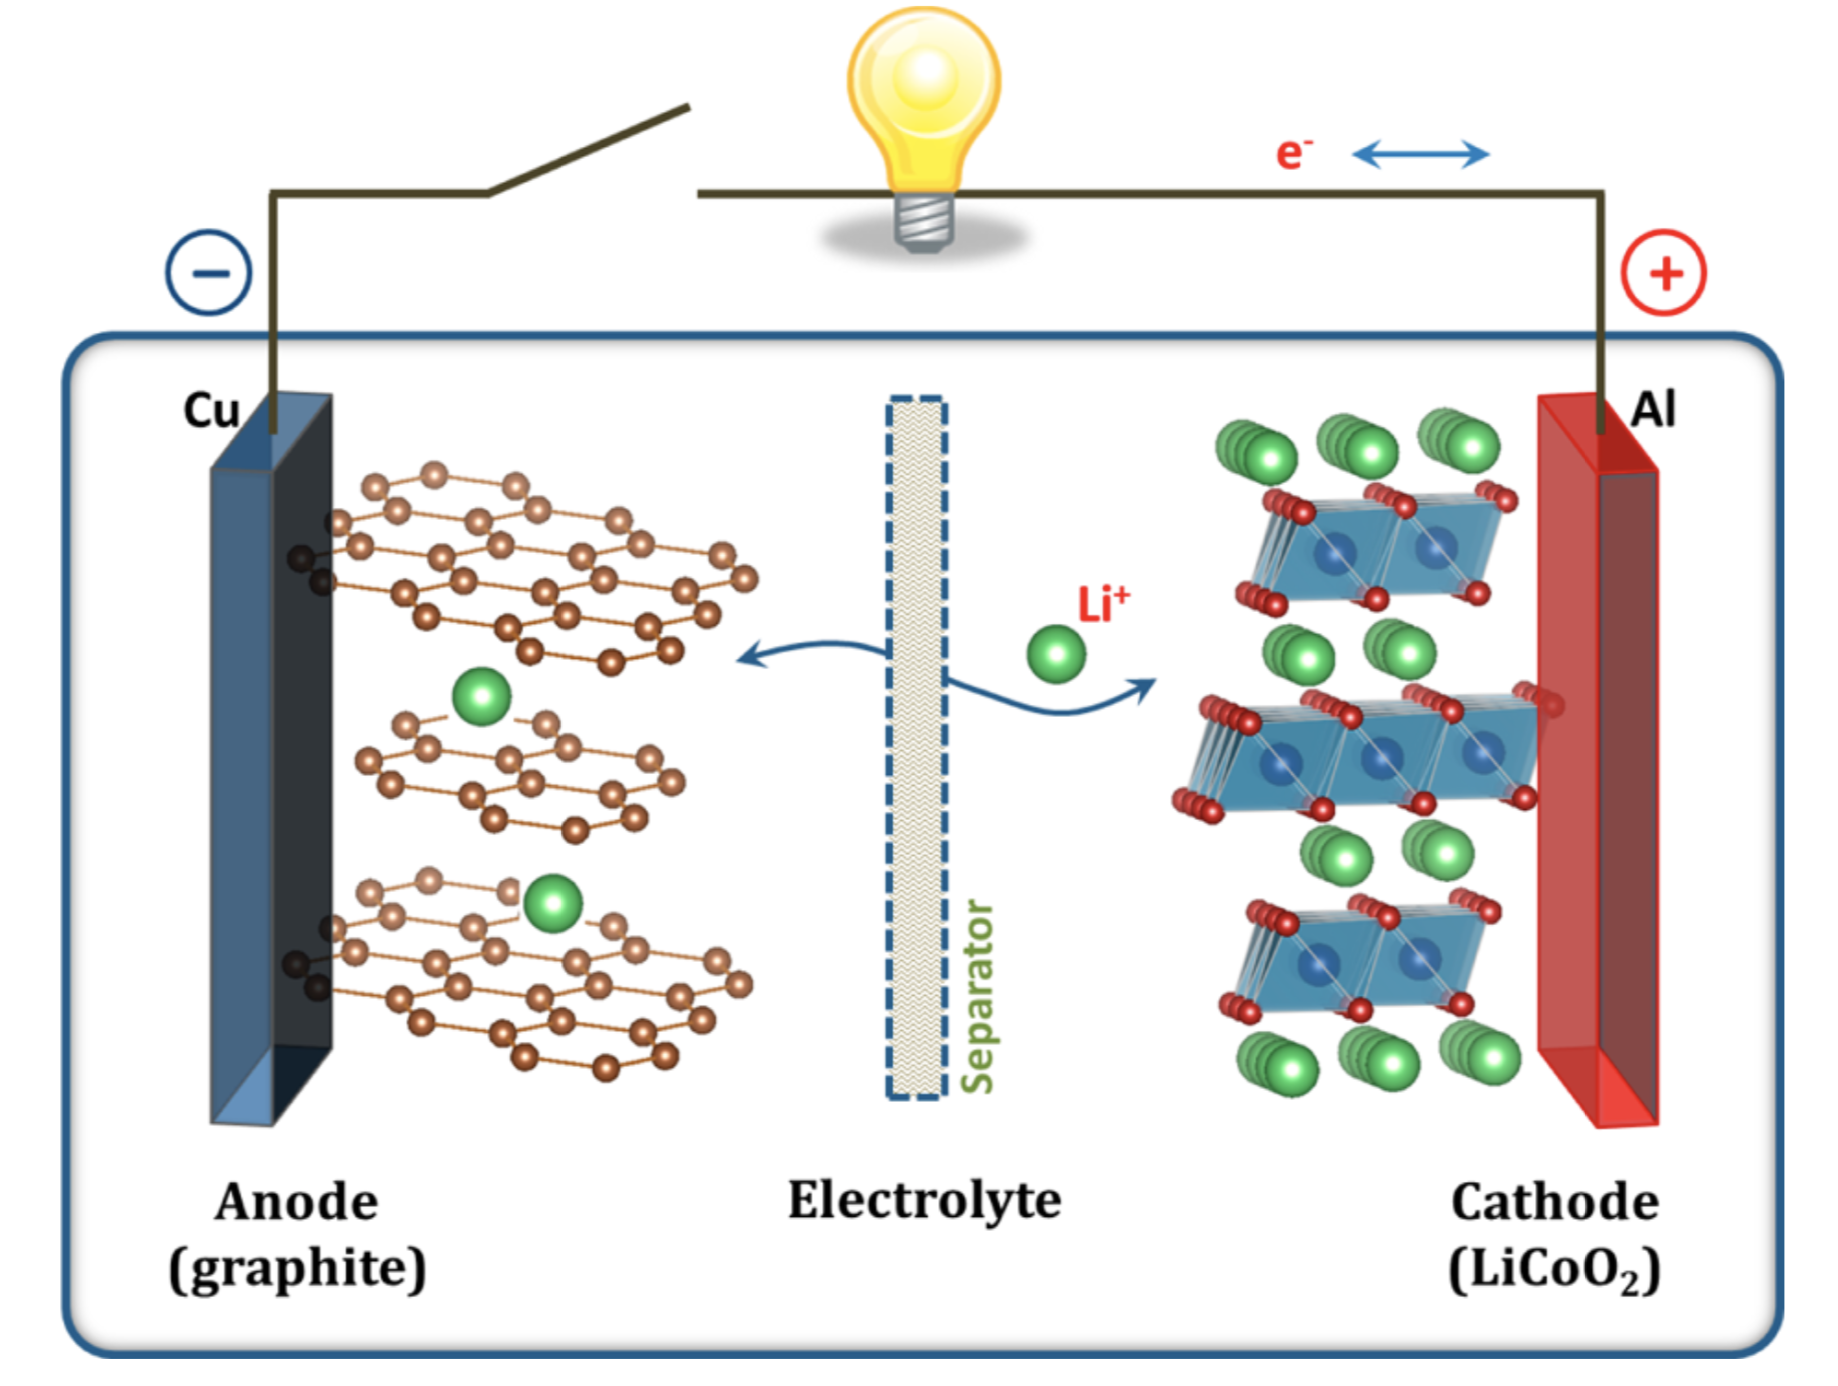
\includegraphics[width=0.7\textwidth]{./figures/batteries/li-ion_battery.png} 
\caption{Basic composition of a Li-ion battery~\cite{Goodenough2013}.} 
\label{batteries:fig-li_ion} 
\end{figure}
 
% When choosing materials for batteries, there are several important properties 
% to consider. First is the ability of the material for storing Li-ions which is 
% best expressed as the specific capacity. # TODO?
 
For the anode, most commercially available \ce{Li}-ion batteries use graphite 
due to its low price, weight and relatively large specific capacity of 
372~\si{\milli\ampere\hour/\gram}~\cite{Mao2018}. Moreover, its layered 
structure is remarkably stable, leading to  a high reversibility and 
cyclability. For the cathode, a more diverse set of materials is being 
considered. The conventional layered oxides \ce{LiMO2}, where \ce{M} is a 
(combination of) transition metals, is still one of the most popular 
chemistries due to their high energy density and rate capacity~\cite{Bresser2015}. Spinel-type 
oxygen-based cathodes~\cite{Thackeray2004} (e.g. \ce{LiMn2O4}) have a lower capacity compared to 
the layered oxides, but are also receiving a fair bit of attention because of 
their excellent safety. Similarly, ordered olivine compounds~\cite{Padhi1997} (e.g. \ce{LiFePO4}) are lauded for their 
high safety and structural stability, but suffer from a reduced specific 
capacity due to their high weight. The electrolyte separating the electrodes 
can be either a liquid or a solid, 
with the liquid being the conventional choice owing to its high ionic 
conductivity. However, there are certain safety hazards associated with the 
use of liquid electrolytes, which has prompted an increased research effort 
for developing functional solid electrolytes (See Section~\ref{batteries:sec-solid_electrolyte}).

\section{Li-Rich Battery Cathodes} \label{batteries:sec-lirich} 
 
Li-ion batteries are currently the primary method of energy storage for many 
important applications, however many potential gains in energy density can 
still be made by improving the cathode capacity. Layered \ce{LiMO2} compounds, 
where \ce{M} is a transition metal, allow for fast two dimensional lithium 
diffusion through a divacancy mechanism~\cite{VanderVen2001}, and high 
voltages versus the battery anode. Among this group, \ce{LiCoO2} has long been 
the favored cathode in commercial applications. Cobalt is expensive and 
toxic, however, and \ce{LiCoO2} suffers from safety problems due to its low thermal 
stability~\cite{Larcher2015}. Moreover, the capacity of \ce{LiCoO2} is limited 
to 130~\si{\milli\ampere\hour/\gram}, because only about half of the lithium 
can be extracted without causing severe electrode 
degradation~\cite{Rozier2015}. 
 
\begin{figure}[ht] 
\centering 
\captionsetup{width=0.9\linewidth}
\begin{tikzpicture}

\definecolor{Li}{RGB}{114, 194, 86}
\definecolor{Co}{RGB}{0, 0, 175}
\definecolor{Mn}{RGB}{168, 8, 158}
\definecolor{Ni}{RGB}{251, 123, 21}
\definecolor{O}{RGB}{254, 3, 0}

% Structures
\node (licoo2) [anchor=west] at (0, 0) {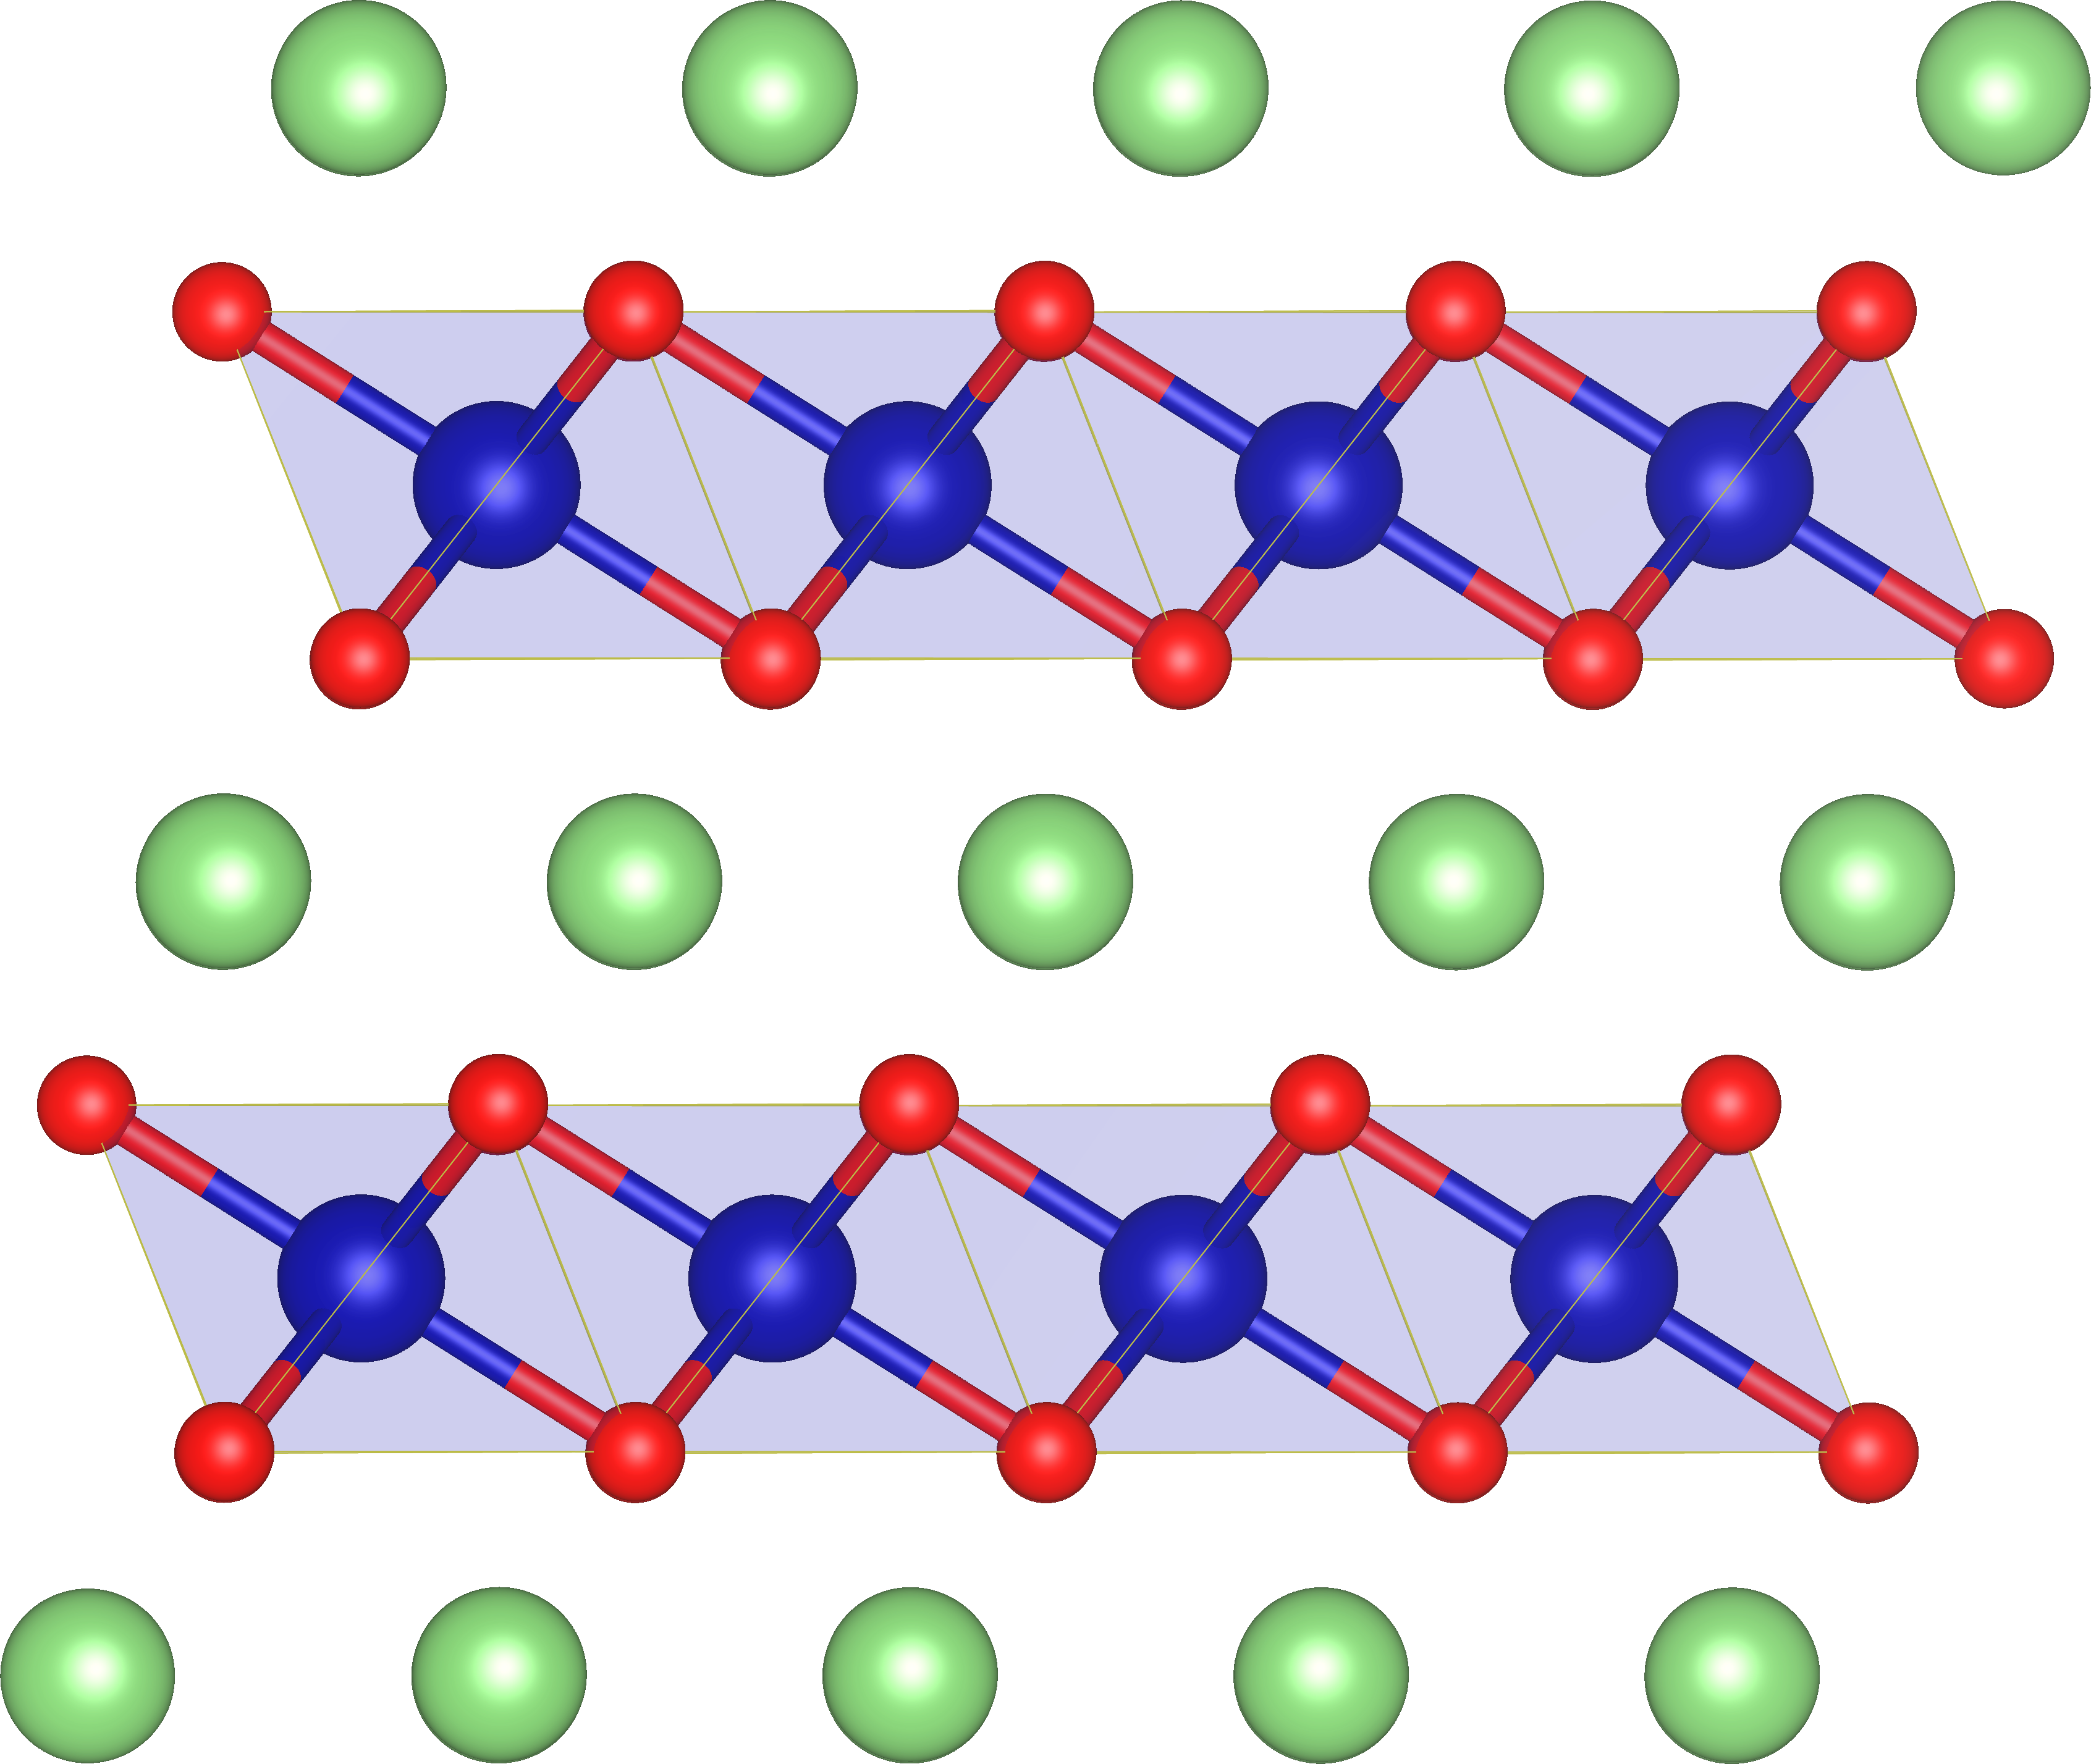
\includegraphics[width=0.26\textwidth]{\figurepath/batteries/diagram_LiCoO2.png}};

% \node (nmc) [] at (0.5\textwidth, 0) {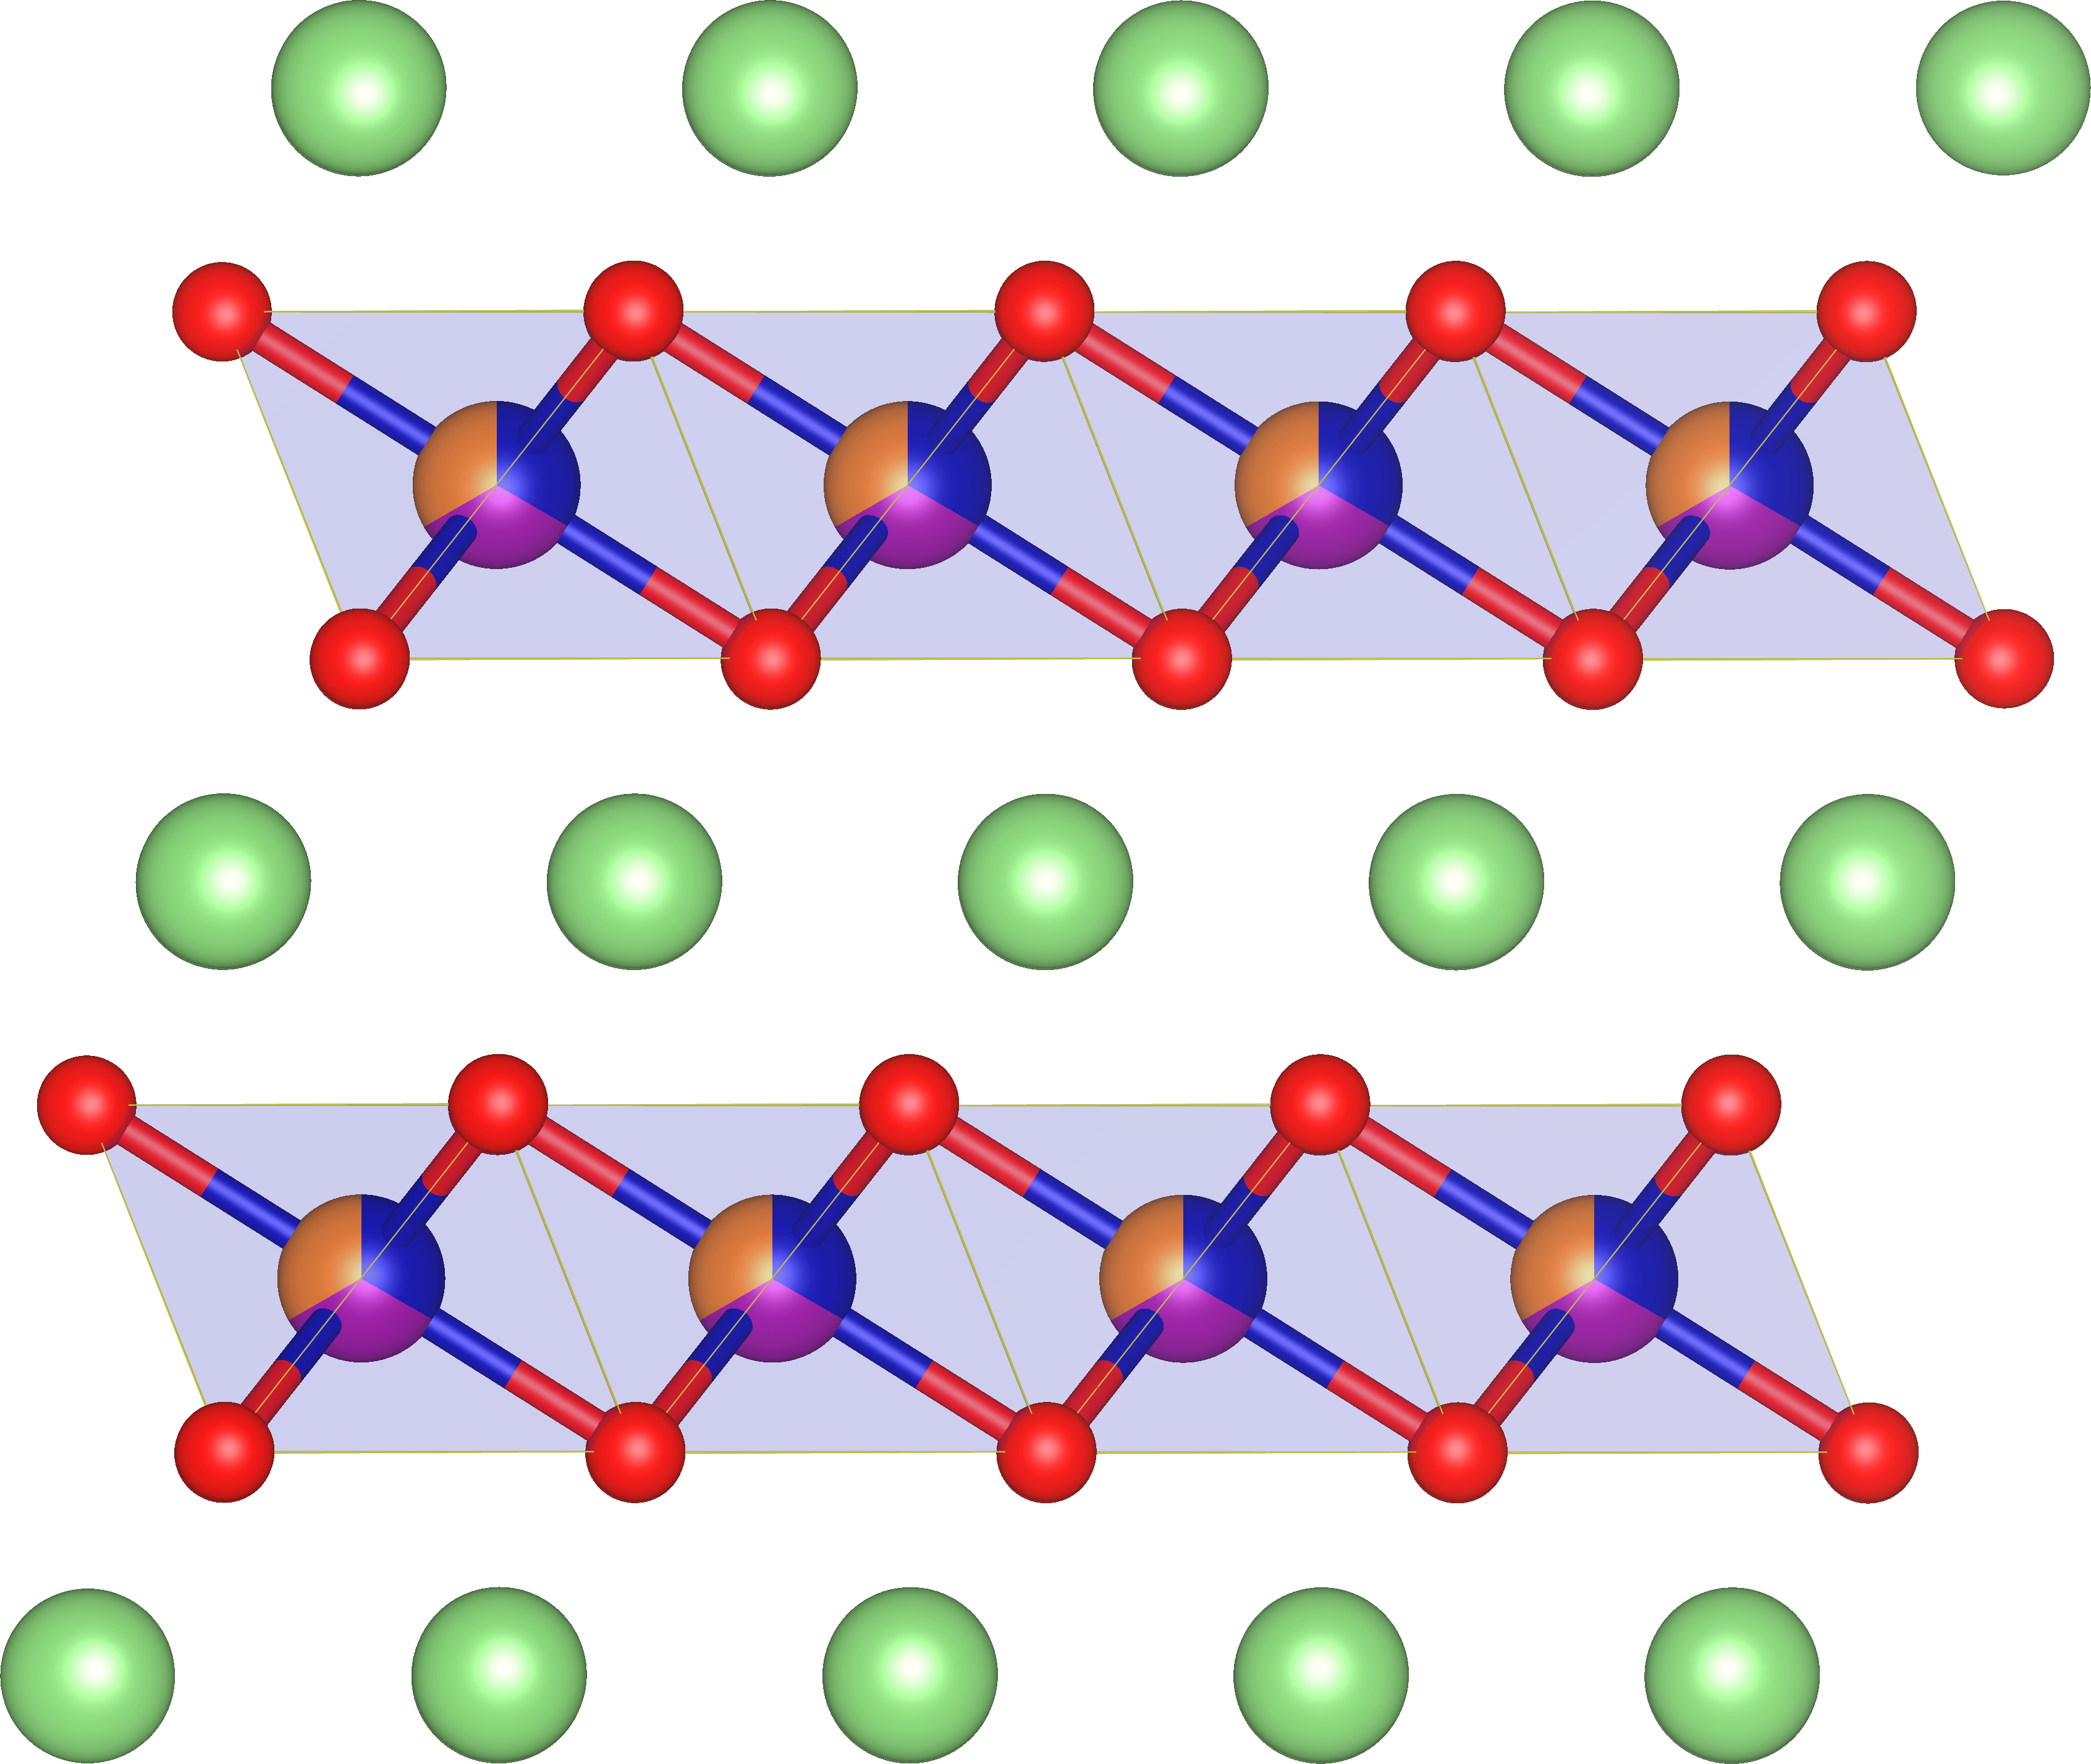
\includegraphics[width=0.26\textwidth]{\figurepath/batteries/diagram_NMC.png}};

% \node (lirich) [anchor=east] at (\textwidth, 0) {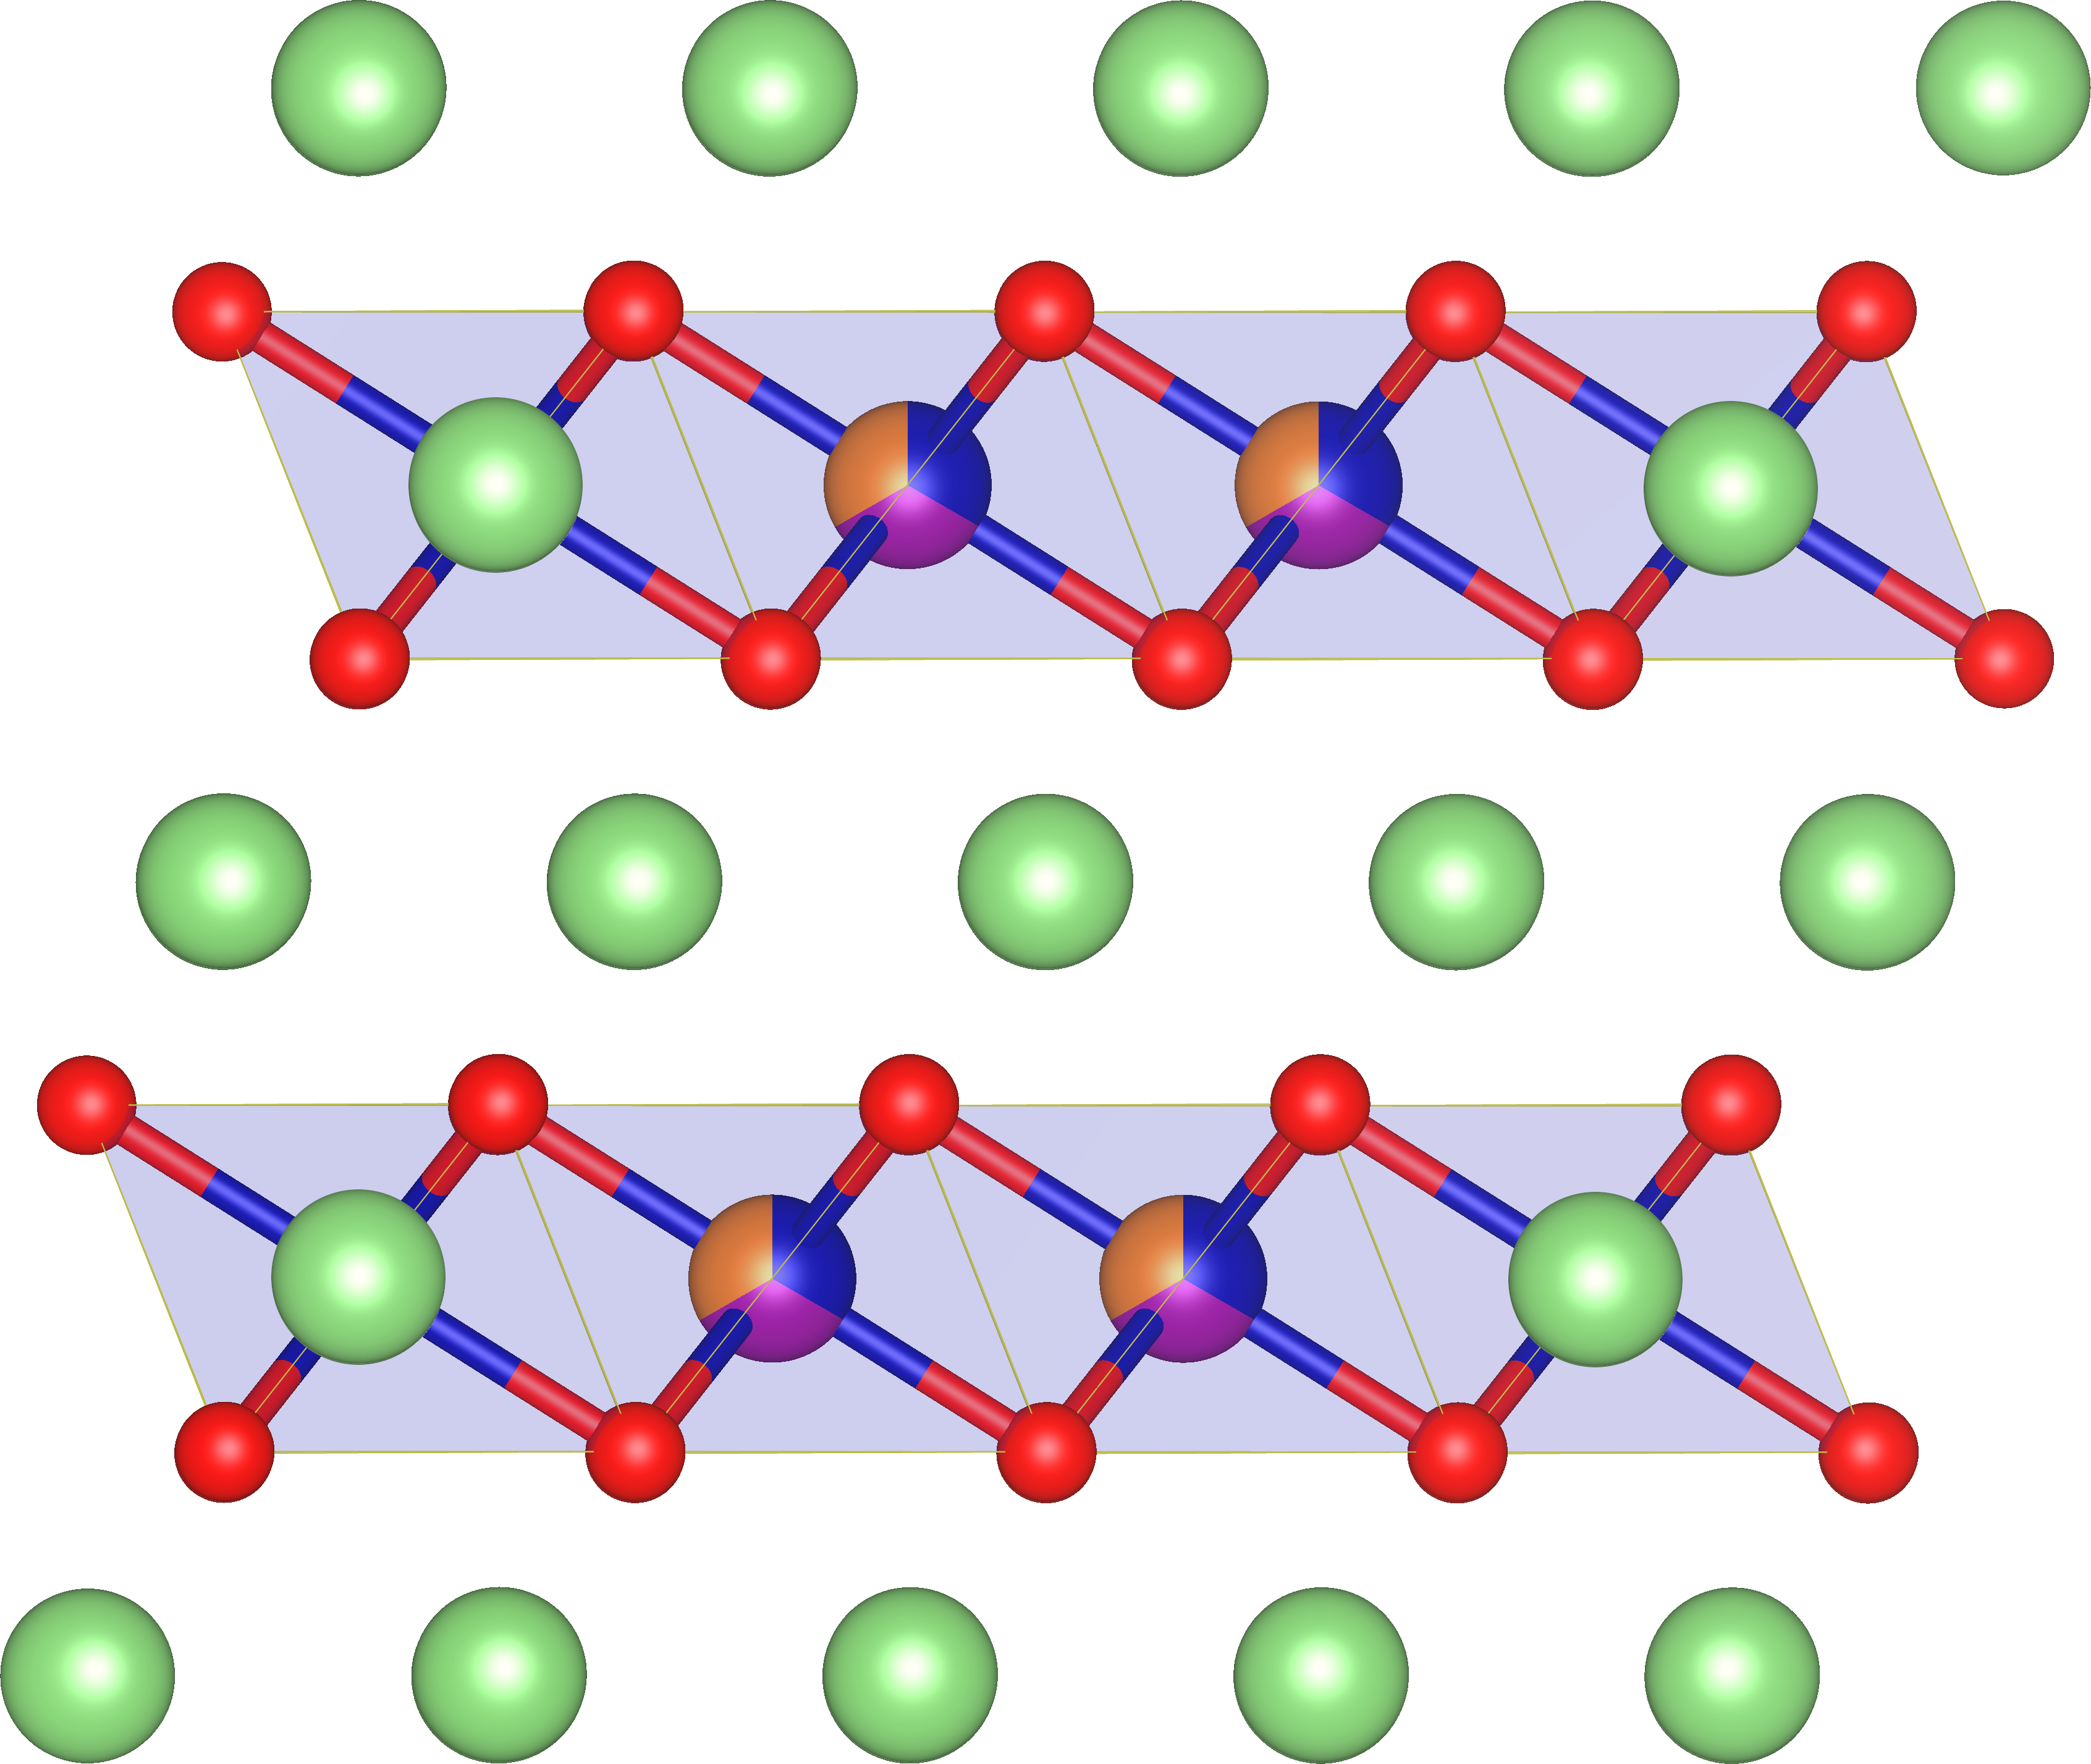
\includegraphics[width=0.26\textwidth]{\figurepath/batteries/diagram_LiRich.png}};

% Arrows
% \node[single arrow, rounded corners=1pt, fill=blue!40!black, draw, anchor=west, minimum width=2em, minimum height=2em] at ($(licoo2)!0.42!(nmc)$) {};

% \node[single arrow, rounded corners=1pt, fill=blue!40!black, draw, anchor=west, minimum width=2em, minimum height=2em] at ($(nmc)!0.42!(lirich)$) {};

% Annotation
\node [anchor=south, font=\Large] at ($(licoo2.north) + (1em, 0)$) {%
\textcolor{Li}{Li}\textcolor{Co}{Co}\textcolor{O}{O}$_2$
};
% \node [anchor=south, font=\Large] at ($(nmc.north) + (1em, 0)$) {%
% \textcolor{Li}{Li}[\textcolor{Ni}{Ni}\textcolor{Mn}{Mn}\textcolor{Co}{Co}]\textcolor{O}{O}$_2$
% };
% \node [anchor=south, font=\Large] at ($(lirich.north) + (1em, 0)$) {%
% \textcolor{Li}{Li}[\textcolor{Li}{Li}\textcolor{Ni}{Ni}\textcolor{Mn}{Mn}\textcolor{Co}{Co}]\textcolor{O}{O}$_2$
% };
\node [anchor=north, font=\bfseries] at ($(licoo2.south) + (0em, 0)$) {%
150~mAh/g
};
% \node [anchor=north, font=\bfseries] at ($(nmc.south) + (0em, 0)$) {%
% 200~mAh/g
% };
% \node [anchor=north, font=\bfseries] at ($(lirich.south) + (0em, 0)$) {%
% 270~mAh/g
% };

\end{tikzpicture}


\caption{Transition from \ce{LiCoO2} to \gls{NMC} to Li-rich layered oxides for 
battery cathodes.} 
\label{batteries:fig-Lirich_transition} 
\end{figure} 
 
In order to improve upon these deficiencies, material scientists have 
attempted chemical substitution of Co by other transition metals such as 
\ce{Mn} and \ce{Ni} (Fig.~\ref{batteries:fig-Lirich_transition}). Since 
\ce{LiNiO2} is deemed unsafe because of its low thermal 
stability~\cite{Ohzuku1993} and \ce{LiMnO2} suffers from poor electrochemical 
performance~\cite{Vitins1997}, researchers use partial substitution of Mn and 
Ni in \ce{LiCoO2} to fine-tune the qualities of the cathode 
material~\cite{Koyama2003}. The resulting \ce{Li[Ni_{1-x-y}Mn_xCo_y]O2} (NMC) 
compounds show improved capacities (200~\si{\milli\ampere\hour/\gram}) and 
safety characteristics, without significantly changing the operating 
voltage~\cite{Zhou2011}.  
 
More recently, further explorations on layered oxide structures have led to 
Li-rich materials, which have an excess of Li in the material 
composition~\cite{Thackeray2007} (Fig.~\ref{batteries:fig-Lirich_transition}). 
These compounds can attain even higher capacities. The origin of this extra 
capacity is believed to be anionic reversible redox processes (\ce{O^{2-}} → 
\ce{O2^{2-}})~\cite{Sathiya2013}, which changes the fundamental minimum of 
transition metal content that was considered necessary in layered oxides for 
decades, and could lead to the next generation of high energy density Li-ion 
batteries. However, these materials still suffer from structural degradation 
as the battery is cycled, reducing the average voltage and capacity of the 
cell. The voltage fade is believed to be related to the migration of 
transition metals into the lithium layer, linked to the formation of O-O 
dimers with a short bond length, which in turn is driven by the presence of 
oxygen holes due to the participation of oxygen in the redox process. Finally, 
the \ce{Li}-rich cathodes have also demonstrated oxygen evolution from the 
structure as the battery is charged, which is detrimental for the safety of 
battery. 
 
This section presents an investigation into the connection between oxygen 
redox and the stability of the oxygen framework for \ce{Li}-rich materials, 
based on \ce{Li2MnO3} and \ce{Li2IrO3}. These two \ce{Li}-rich cathode 
materials have demonstrated significantly different cycling properties. 
\ce{Li2MnO3}, a well studied \ce{Li}-rich material, suffers from a substantial 
amount of voltage fade as the battery is cycled~\cite{Croy2014}, whereas 
\ce{Li2IrO3} does not~\cite{McCalla2015}. Studying the differences in 
oxidation and structural stability between these two compounds can offer 
insight as to why their cycling properties are so different.  
 
\resultsubsection{Structure and Li configuration \label{batteries:sec-structure}}{https://github.com/mbercx/phd-thesis/tree/master/jupyter/batteries/README.md\#structure-and-li-configuration}{structure} 

In order to compare the structural stability of the oxygen framework for the 
\ce{Li2MnO3} and \ce{Li2IrO3} compounds, we have to calculate the chemical 
reaction energy for the formation of O-O dimers for both cathode materials in 
a charged state, i.e. after the removal of a certain fraction of lithium. 
However, the fully charged structure for \ce{Li2MnO3} is found to be highly 
unstable, i.e. lead to the spontaneous formation of several oxygen dimers, 
especially when any local changes to the structure are made. Moreover, the 
cathode is unlikely to ever be fully delithiated in a practical battery, 
rendering an investigation of the fully charged state less relevant. 

\begin{figure}[ht] 
\centering
\captionsetup{width=0.9\linewidth}
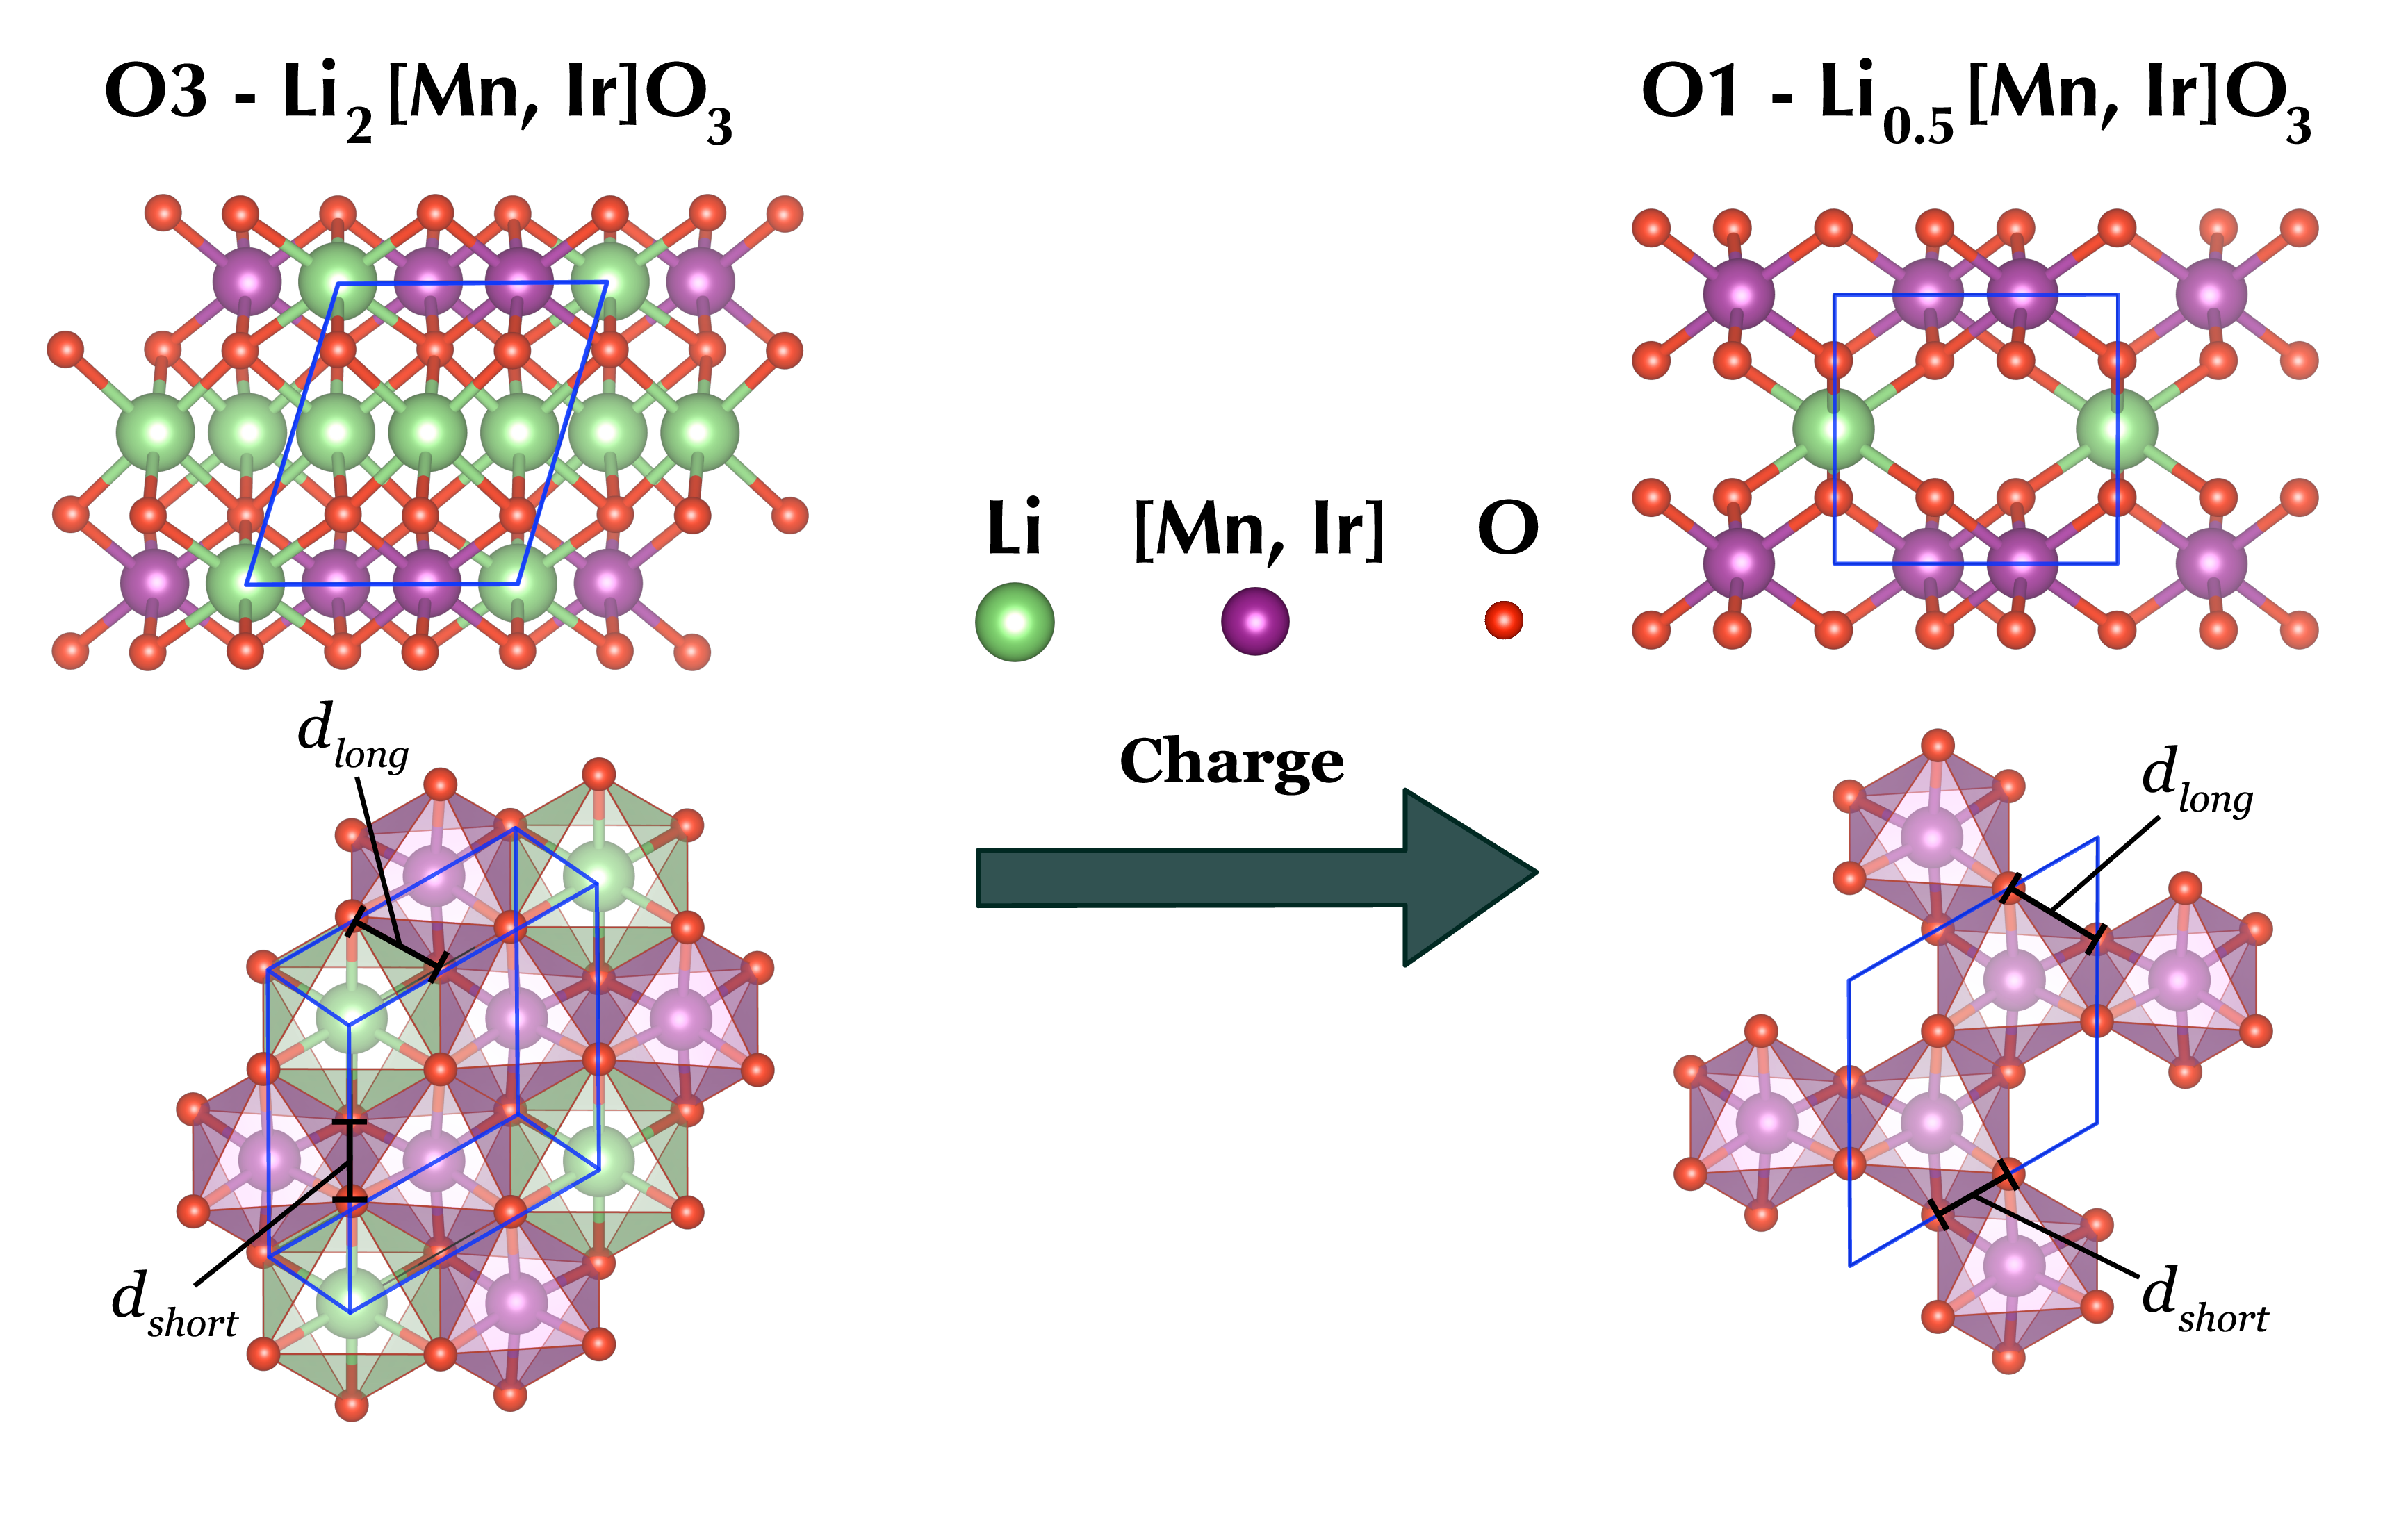
\includegraphics[width=0.80\textwidth]{figures/batteries/structural_change.png} 
\caption{Transformation from the O3 to O1 stacking for both \ce{Li2MnO3} and 
\ce{Li2IrO3} as the cathode is charged. The primitive unit cell 
is drawn in blue. The top figures represent the structure shown in the [100] 
projection, whereas the lower figures represent a single octahedral layer of 
the layered structure, viewed top down.  $d_{short}$ and $d_{long}$ both 
represent O-O distances across the \ce{Li}/TM layer, corresponding to an 
octahedral edge bordering two \gls{TM}'s and a \gls{TM} and \ce{Li}/Vacancy, respectively.} 
\label{batteries:fig-structural_change} 
\end{figure} 

Hence, the structural stability should preferably be studied in a partially 
charged cathode material. This requires knowledge about the location of the 
lithium for each state of charge, as there are many possible \ce{Li}-Vacancy 
configurations to consider. We investigate the lithium configuration for 
\ce{Li2MnO3} by calculating the energy of all symmetrically non-equivalent 
configurations in the conventional unit cell. This is done based on the 
workflow described in Section~\ref{automation:sec-configurations}, resulting 
in 94 non-equivalent configurations. Similar to previous 
work~\cite{Koyama2009}, we find that for several lithium configurations, 
the \ce{Li2MnO3} structure spontaneously shifts from an O3 stacking to the O1 
stacking\footnote{The various stackings of layered oxides were first classified 
by Delmas et al.~\cite{Delmas1980}. O refers to the octahedral coordination 
of O atoms around the alkali (Li, Na, ...) ions. The number is related to 
the stacking of the O atoms, i.e. for O3 the stacking is AB CA BC, so after 
3 layers of alkali ions, the oxygen environment returns to its original 
stacking. For O1, the stacking is AB AB, so the stacking for each alkali 
layer is the same.} at higher charge state of the battery 
(see Fig.~\ref{batteries:fig-structural_change}). In order to verify this transition from 
the O3 to the O1 stacking, we once again use the configuration workflow to 
calculate the energy of all \ce{Li} configurations in unit cells up to two 
times the size of the conventional unit cell of the O1 stacking, which results 
in 220 non-equivalent configurations. 

For the O1 stacking, we find that 
several configurations at lower states of charge switch to the O3 stacking, 
i.e. the opposite transformation occurs compared to that at higher states of 
charge. To be able to compare the energies of the O1 and O3 stackings fairly, we 
remove the configurations which change stacking. As the stacking 
of the oxygen octahedra is closely connected to the angles between the 
lattice vectors, we remove all configurations for which any lattice angle has 
changed more than 12\si{\degree}. This leaves 84 and 181 configurations for 
the O3 and O1 stacking, respectively. Finally, we calculate the formation 
energy for all configurations versus the fully charged and discharged state of 
the O3 stacking: 
\begin{equation} 
E_f (x) = E(\ce{Li_xMnO3}) - (1 - \frac{x}{2}) E(\text{O3-}\ce{MnO3}) - 
\frac{x}{2} E(\text{O3-}\ce{Li2MnO3}) 
\end{equation} 
The corresponding formation energies are plotted for both stackings in 
Fig.~\ref{batteries:fig-li_configuration}. It is clear that as \ce{Li} is 
removed from \ce{Li2MnO3}, the O1 stacking becomes thermodynamically 
favorable. 
 
\begin{figure}[ht] 
\centering
\captionsetup{width=0.9\linewidth}
\begin{tikzpicture}

\begin{axis}[
width=0.35\textwidth, height=5cm,
tick align=inside,
tick pos=left,
xtick={0, 0.5, 1.0, 1.5, 2.0},
xticklabels={0, 0.5, 1.0, 1.5, 2.0},
x grid style={white!69.0196078431373!black},
xlabel={$x$ in Li$_{2-x}$\ce{MnO3}},
xmin=0.0, xmax=2.0,
xtick style={color=black},
y grid style={white!69.0196078431373!black},
ylabel={$E_f$ (meV/f.u.)},
ymin=-500, ymax=450,
ytick style={color=black}, mark options={line width=1pt},
legend style={
at={(1, 1)}, anchor=north east, draw=none, fill=none, 
},
]
% This file was created by tikzplotlib v0.9.1.
\definecolor{color0}{rgb}{0.0862745098039216,0.23921568627451,0.36078431372549}
\definecolor{color1}{rgb}{0.72156862745098,0.12156862745098,0.12156862745098}

\addplot [only marks, mark=x, draw=color0, fill=color0, colormap/viridis, forget plot]
table{%
x                      y
1.5 -67.8026499999991
1.5 -71.5859850000005
0 0
0.25 -23.0760987500034
0.5 -15.8183675000032
0.25 -18.8248337499957
0.5 -33.0075625000035
0.75 20.4665637500021
0.25 5.04160125000652
0.5 -26.9582499999999
0.75 -13.3455562499982
1.5 -13.5087800000004
0.5 -47.9653850000048
0.75 -65.7496287500017
1 23.1862824999993
0.5 -57.7858600000027
0.5 -39.2016549999994
0.75 -38.8773887499987
0.5 -33.7245824999997
0.75 -55.5752012499973
0.75 -12.5851312500025
1 9.94340500000135
0.5 -74.1484475000007
0.75 -103.802866249996
0.75 -88.582366249998
1 -78.7985900000017
0.75 -104.837603750003
1 -114.657662500001
1 -95.7689449999997
1.25 -20.3259112500014
1 -31.1918700000007
0.75 -22.2435537499983
1 -8.33987000000036
1.25 15.2983287499993
0.75 -101.364936249997
1 -118.287705
1.25 -106.433326250002
1 -111.1227325
1.25 -89.9410337500015
1.5 -19.3536775000016
0.5 -57.0251500000012
0.75 -57.7473962499973
1.5 -112.0246725
1 4.72285000000028
0.5 -34.7879000000049
0.75 -52.6830512499963
1 -32.2887999999999
0.75 -105.359046249998
1 -95.9716300000011
1.25 -10.7871537500017
1 -64.5238050000003
1 -39.1175075000021
1.25 17.864861249997
0.75 -84.3509437499996
1 -95.7160600000009
1 -72.4130149999986
1 -133.199690000001
1.25 -115.11746875
1.25 -106.09587375
1.5 -12.8744375000007
1 -42.1860150000022
1.25 -57.4472487500017
1.5 -18.654419999999
1.25 -62.6492362500031
0.5 -10.3780525000019
0.75 -77.1715362500025
1 -86.3607799999997
0.75 -65.7122187499972
1 -96.6504075000003
1.25 -27.0222787499996
1 -145.6501925
1.5 -183.354082500001
1 -138.4063225
1.25 -151.877863750002
1 -112.511452500001
1.25 -140.207731250001
1.25 -125.249346250001
1.5 -71.5056275000006
1.25 -104.846703750002
1.5 -112.033797499999
1 -152.272
1.25 -166.87082875
1.5 -67.8254575000015
2 0
};
\addplot [only marks, mark=x, draw=color1, fill=color1, colormap/viridis, forget plot]
table{%
x                      y
1.5 -35.7198450000009
1.5 13.8671950000013
1.5 5.66435250000019
1.5 -136.42538
1.5 -148.1757525
1.5 -466.37087
1.5 -466.00319
1.5 -37.4475125
1.5 63.0465524999995
1.5 -466.283540000001
1.5 8.0885850000012
1.5 -16.1756499999992
1.5 -64.0798475000022
1.5 -91.801757499999
1.5 -208.248365000001
1.5 -466.270182499999
1.5 3.24785499999969
0.75 27.7692387500004
0.75 -65.4409062500001
1 -14.6044250000017
0.5 106.422629999997
0.75 33.2896162499985
0.75 64.1449112500005
0.75 -28.9037412500015
1 -147.332670000001
0.75 9.48292125000094
1 -46.2707000000009
1 -147.216132499999
1 -49.1448900000009
0.75 60.4110862500029
1 -50.1839574999998
1 20.9184974999985
1.25 -276.374341250001
1.25 -252.558533750001
1.25 -146.766116250003
1.5 -465.922040000001
0.75 128.836908749999
1 -118.859632500001
1.25 -43.744151250003
1 -83.2892224999995
1.25 -277.11238625
1.25 -277.256591250001
1.25 -76.8601787499996
1.5 -148.095979999999
1.5 -136.691324999999
1.75 -278.29735875
1 59.8648299999986
1.25 23.8585037499988
1 51.8307424999982
1.25 55.8417387499972
1.5 4.31360499999833
1.75 -42.9858537500012
1.5 3.74343999999915
1.75 -31.753881250002
0.25 278.067671250007
0.25 366.577636250007
0.5 209.917387499999
0.5 204.486254999999
0.75 3.05097875000016
0.25 283.564511249999
0.5 211.315567499994
0.5 285.543279999999
0.75 1.49343624999787
0.75 178.344966250002
0.5 195.933697499996
0.75 87.6730062500037
0.75 101.97282375
1 -43.1307475000011
0.75 154.44530625
1 67.6516850000013
1.25 51.7273287499975
0.75 80.9546087500017
1 -74.8433175000009
0.75 -4.30096874999819
1 -13.2827100000021
1.25 -210.445518750003
1.25 39.7558837499972
1.5 -0.067079999999109
0.75 157.699693750001
1 -28.8397750000016
0.5 210.866732500001
0.75 3.41788375000007
0.75 130.252321250001
0.75 229.812958749999
1 -29.7932050000007
1 121.373389999999
1.25 -16.7678562500022
1 11.3948525000005
1.25 -163.314961250002
1 -77.082282500001
1 45.2134075000004
1.25 -76.771101250003
1.5 -46.8126874999992
1.25 21.5352862499998
1.5 -47.3177300000014
1 -84.5194900000017
1.25 -210.183833750001
1.25 -156.006766250002
1.5 -465.774582500002
1.75 -268.687781249999
1.5 2.5161074999982
0.75 152.688718749999
1.25 17.6442987499996
1.25 1.50469624999872
1.5 65.2503999999983
1.5 -221.161452500001
1.75 -43.0172587499991
1.75 27.0933737499979
0 402.592247500003
0.5 189.620729999994
1 -13.0468824999994
0.5 319.712344999999
1 14.4232624999994
0.5 186.135019999995
1 130.895007500001
1 118.8892425
1.5 -33.9014399999993
2 -92.5534025000019
0.25 274.729598750007
0.5 169.467679999997
0.25 256.158468750009
0.5 113.974772500001
0.75 -75.739386249996
0.25 256.909133750007
0.5 228.516722499997
0.75 179.44924875
0.5 232.899677500001
0.75 147.289118749999
1 84.3360400000002
0.5 101.40603
0.75 50.136783750002
0.75 75.2846687499975
0.75 -11.8587562499961
1 -134.4995
0.5 96.2923199999963
0.75 109.194606250004
0.75 24.9466412500006
1 30.9840675000004
0.75 78.3939737499999
1 20.8507400000002
1 -15.4031225000004
1.25 -251.212456250002
1.25 -255.280936250003
0.75 -81.9174362499986
1 -126.957332500002
1.25 -135.231771250002
1 -120.292895000002
1.25 -251.354438750003
1.5 -466.162877500002
0.75 143.298301250002
1 -82.7219200000009
0.75 233.610356250001
1 151.192209999998
1.25 97.1316512499989
1 -66.1910150000011
1.25 -251.56119375
1 58.2182375000002
1.25 15.7311662499993
1.25 -51.7610287500005
1.5 -64.0674749999999
1.25 -131.559473750002
1.5 -208.130025000001
1.75 -257.29269375
0.75 131.129783750001
1 77.526044999999
0.75 152.883083750002
1 81.6482249999986
1.25 30.8078262499976
1 38.4612900000008
1.25 46.5428287499989
1.25 45.8883112499997
1.25 -26.9648862500027
1.5 -15.0176300000009
1.75 -41.2600712500018
1.25 30.9845512500004
1.5 8.97925000000122
1.75 -65.50583875
0.25 253.497913750003
0.5 132.739534999999
0.75 -65.659388750003
0.5 144.126992499999
};
\addplot [semithick, color0, mark=square*, mark size=1.5, mark options={solid}]
table {%
0 0
1 -152.272
1.5 -183.354082500001
2 0
};
\addlegendentry{O3}
\addplot [semithick, color1, mark=square*, mark size=1.5, mark options={solid}]
table {%
0 402.592247500003
0.75 -81.9174362499986
1.5 -466.37087
2 -92.5534025000019
};
\addlegendentry{O1}

\end{axis}

\end{tikzpicture}

\caption{Formation energies of all configurations in both the O3 and O1 
stacking of \ce{Li_xMnO3}. Each mark represents the formation energy of one non-equivalent Li configuration. The full lines correspond to the convex hull of the 
corresponding stacking.} 
\label{batteries:fig-li_configuration} 
\end{figure} 
 
A similar transformation from the O3 to O1 stacking is found to occur for 
\ce{Li_{0.5}IrO3}, which has been experimentally verified and leveraged in 
order to study the deformation of the oxygen framework by McCalla et 
al.~\cite{McCalla2015}. This means that structures of the discharged and 
charged structures are the same, save for a difference in the lattice 
parameters, which facilitates the comparison of the changes in geometry and 
oxidation state between \ce{Li2MnO3} and \ce{Li2IrO3}. We choose to focus on 
the 75\% charged structures for several reasons. First, the optimal lithium 
configuration for \ce{Li_{0.5}MnO3} is on the convex hull of the O1 stacking, 
indicating that this structure is quite stable and hence easier to work with 
once we start introducing O-O dimers (Sec.~\ref{batteries:sec-dimer}). Second, 
oxygen gas is only released from the \ce{Li2IrO3} cathode once it is charged 
beyond 75\%~\cite{McCalla2015}, whereas \ce{Li2MnO3} has already lost oxygen at this state of 
charge~\cite{Castel2014}. Hence, studying the stability for this lithium content is most 
interesting, as it may show discrepancies between the stability of the oxygen 
frameworks. Finally, the oxygen framework of \ce{Li_{0.5}IrO3} was studied by 
McCalla et al.~\cite{McCalla2015}, which allows for a direct comparison of our 
calculated O-O distances with experiment. 

\begin{table}[ht] 
\centering 
\captionsetup{width=0.9\linewidth}
\renewcommand{\arraystretch}{1.3} 
\caption{O-O distances for the discharged and charged \ce{Li2[Mn, Ir]O3} 
structures, all expressed in \AA. The distances for \ce{Li2IrO3} are compared 
with the neutron powder diffraction results of McCalla et 
al.~\cite{McCalla2015}.} 
\label{batteries:tab-OO_distance} 
\begin{tabular}{c c c c c c c} 
 & & \multicolumn{2}{c}{\ce{Li2[Mn, Ir]O3}} & & 
\multicolumn{2}{c}{\ce{Li_{0.5}[Mn, Ir]O3}}\\\cline{3-4}\cline{6-7} 
 & & \gls{DFT} & Neutron & & \gls{DFT} & Neutron \\\hline 
\multirow{2}{*}{Mn} & \multicolumn{1}{|c}{$d_{short}$} & 2.52 & - & & 2.31 & - 
\\ 
 & \multicolumn{1}{|c}{$d_{long}$} & 2.75 & - & & 2.62 & - \\\hline 
\multirow{2}{*}{Ir} & \multicolumn{1}{|c}{$d_{short}$} & 2.75 & 2.77 & & 2.51 
& 2.45 \\ 
 & \multicolumn{1}{|c}{$d_{long}$} & 2.87 & 2.84 & & 2.74 & 2.73 \\\hline 
\end{tabular} 
\end{table} 
 
As was noted previously by McCalla et al.~\cite{McCalla2015}, the oxygen 
framework is distorted as lithium is removed from the structure. In order to 
quantify this, we calculate the distances between the various oxygen pairs, 
connected in the tetrahedral environment of \ce{Mn} or \ce{Ir}. The distances 
between oxygen pairs which are part of the same oxygen layer change little. 
However, for the interlayer oxygen pairs, denoted as $d_{short}$ and 
$d_{long}$ in Fig.~\ref{batteries:fig-structural_change}, the change in bond 
length is more pronounced (Table~\ref{batteries:tab-OO_distance}). Moreover, 
the shorter bonds for an oxygen pair sharing two [Mn, Ir] neighbors, shrink 
more than the long bonds, which share a transition metal and Li or vacancy. 
This leads to a distortion of the octahedral environment around the transition 
metals, resulting in short O-O bonds which McCalla et al. refer to as dimers. 
In Section~\ref{batteries:sec-dimer}, we will return to this topic, focusing 
our attention on the formation of a peroxo species with a bond length closer 
to that of the oxygen molecule, as this formation has been derived 
theoretically for \ce{Li2MnO3}, and believed to be related to the migration of Mn 
and the resulting voltage fade~\cite{Chen2016}. 

\resultsubsection{Oxidation \label{batteries:sec-oxidation}}{https://github.com/mbercx/phd-thesis/tree/master/jupyter/batteries/README.md\#oxidation}{oxidation} 
 
Sathiya et al.~\cite{Sathiya2013} have discussed that removing lithium from 
\ce{Li}-rich cathodes leads to the formation of holes on the oxygen, i.e. the 
oxidation of oxygen. Seo et al.~\cite{Seo2016} have proposed that the 
formation of localized holes relies on the presence of labile oxygen states, 
which are found for oxygen with \ce{Li} atoms on opposite sites of its 
octahedral environment. Moreover, they explain that because of the honeycomb 
structure of \ce{Li2MnO3}, all oxygen environments have such a 
\ce{Li}-\ce{O}-\ce{Li} configuration, leading to a high participation of 
oxygen in the redox processes. Although \ce{Li2IrO3} has a similar structure, 
Hong et al.~\cite{Hong2019} assert that because \ce{Ir^{4+}} can be more 
easily oxidized, these labile oxygen states are not depleted to the same 
extent, stabilizing the oxygen framework. 
 
\begin{table}[ht] 
\centering
\captionsetup{width=0.9\linewidth}
\renewcommand{\arraystretch}{1.3} 
\caption{Calculated absolute values of the magnetic moments for the discharged 
and charged \ce{Li2[Mn, Ir]O3} structures, all expressed in Bohr magnetons $\mu_B$. Note that 
for the \ce{Ir} structures, non-collinear calculations were performed to include spin-orbit coupling, and the norm of the local magnetization vector was calculated in order to 
express the local magnetic moment as a scalar.} 
\label{batteries:tab-magmoms} 
\begin{tabular}{c c c c} 
 & & \ce{Li2[Mn, Ir]O3} & \ce{Li_{0.5}[Mn, Ir]O3} \\\hline 
\multirow{2}{*}{Mn} & \multicolumn{1}{|c}{$|\mu|$ (\ce{Mn})} & 2.918 & 2.949 
\\ 
 & \multicolumn{1}{|c}{$|\mu|$ (\ce{O})} & 0.001 & 0.445  \\\hline 
\multirow{2}{*}{Ir} & \multicolumn{1}{|c}{$|\boldsymbol{\mu}|$ (\ce{Ir})} & 0.374 & 1.025 
\\ 
 & \multicolumn{1}{|c}{$|\boldsymbol{\mu}|$ (\ce{O})} & 0.025 & 0.314 \\\hline 
\end{tabular} 
\end{table} 
 
To study the change in the oxidation state of the atoms, we compare the 
calculated local magnetic moments of the various elements for both structures 
in the discharged and 75\% charged state in Table~\ref{batteries:tab-magmoms}. 
Note that as \ce{Ir} exhibits strong spin-orbit coupling effects, non-collinear 
calculations were performed for both \ce{Li2IrO3} and \ce{Li_{0.5}IrO3}.
We can see that for \ce{Li2MnO3}, the magnetic moment of Mn remains largely 
the same, whereas the magnetic moment on oxygen increases significantly. For 
oxygen, the increase in magnetic moment corresponds to an oxidation from its 
\ce{O^{2-}} state, as its $p$-orbitals are no longer fully occupied, leading 
to an increased local density of unpaired electrons. The results for \ce{Mn} 
indicate that it does not participate much in the redox processes that occur 
when the battery is charged. Instead, its magnetic moment remains close to 3 
$\mu_B$, which corresponds to the initial oxidation state \ce{Mn^{4+}} in the 
discharged cathode structure. For \ce{Li2IrO3}, removing lithium from the 
discharged structure results in a significant change of the local magnetic 
moment for both \ce{Ir} and \ce{O}, implying a more mixed redox process during the 
charging of the cathode. This mixed redox for \ce{Li2IrO3} is in agreement 
with the X-ray photoelectron spectroscopy results of McCalla et al.~\cite{McCalla2015}, where they explain 
that this is in part due to the covalent character of the Ir-O bond. This 
covalency could also explain why oxygen is oxidized less when charging 
\ce{Li2IrO3}, as valence electrons are removed from both Ir and O. 
\ce{Mn^{4+}} could in principle also be oxidized further, but the \ce{Mn^{5+}} 
oxidation state is rare, and generally not octahedrally 
coordinated~\cite{Saint2007}. The fact that the change in magnetic moment on O 
is smaller for \ce{Li2IrO3}, than for \ce{Li2MnO3} indicates that the mixed 
redox process in the charging of \ce{Li2IrO3} results in a lower state of 
oxidation for the oxygen of the structure in the charged state.  
 
\begin{figure}[ht] 
\centering 
\captionsetup{width=0.9\linewidth}
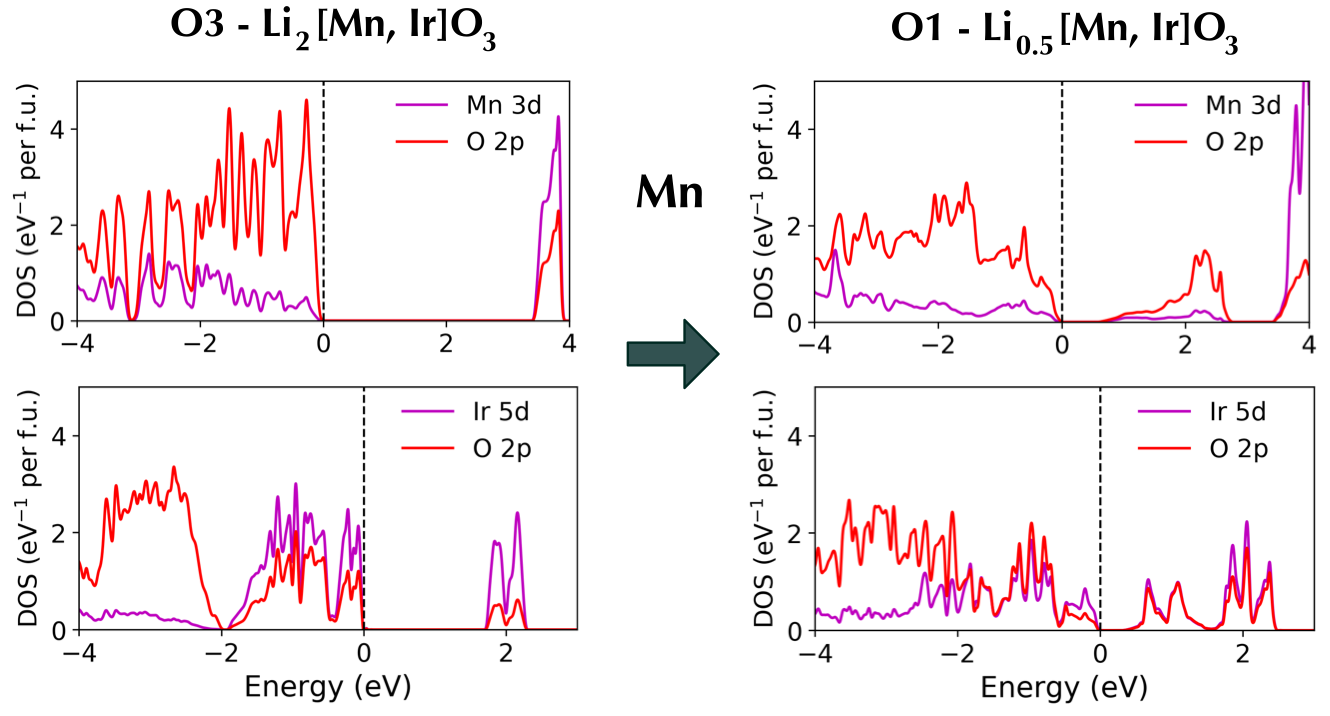
\includegraphics[width=\textwidth]{Figures/batteries/charge_pdos_Mn_Ir.png} 
\caption{The projected density of states of the Mn-3$d$, Ir-5$d$ and O-2$p$ 
orbitals for the discharged (left) and charged (right) structures, where we 
have aligned the Fermi level to zero. In order to allow for a reasonable 
comparison between the pristine and charged state, we have consistently 
plotted the number of states per electronvolt per formula unit.} 
\label{batteries:fig-charge_pdos_Mn_Ir} 
\end{figure} 
 
This conclusion is supported by the projected density of states (\gls{PDOS}), 
plotted in Fig.~\ref{batteries:fig-charge_pdos_Mn_Ir}. For \ce{Li2MnO3}, the 
electronic states close to the Fermi level correspond largely to the O-2$p$ 
states, which indicates that as the battery is charged, electrons are removed 
from oxygen rather than \ce{Mn}. In contrast, looking at the \gls{PDOS} for 
\ce{Li2IrO3} reveals that the states near the Fermi level are more evenly 
distributed between O-2$p$ and Ir-5$d$, which corresponds well to the picture 
of a more mixed redox activity for this material. When comparing the \gls{PDOS} of 
the charged structures with the discharged ones, we note that in both cases 
the number of O-2$p$ states near the Fermi level has decreased. The difference 
is much more substantial for \ce{Li2MnO3} than for \ce{Li2IrO3}, once again 
implying a larger oxidation of oxygen for \ce{Li2MnO3}. 

\pagebreak
\resultsubsection{Dimer Analysis \label{batteries:sec-dimer}}{https://github.com/mbercx/phd-thesis/tree/master/jupyter/batteries/README.md\#dimer-analysis}{dimer} 
 
Once the oxygen atoms develop holes on their $p$-orbitals, they can be 
subsequently stabilized by a reorganization of the oxygen framework, forming a 
peroxo-like species of oxygen pairs with shortened O-O bonds. McCalla et 
al.~\cite{McCalla2015} were able to demonstrate the shortening of such bonds 
for \ce{Li2IrO3}, which they referred to as an O-O peroxo-like dimer. More 
recently, other authors~\cite{Saubanere2016, Chen2016} have asserted that the 
presence of unstable holes on the oxygen can also lead to the formation of a 
true oxygen dimer, finding O-O bonds with distances closer to that of 
molecular oxygen (~1.3-1.5~\si{\angstrom}). Such short O-O distances have also 
been reported recently by Li et al.~\cite{Li2018}, who found shifts in their 
Raman spectra that correspond to similar bond lengths. Both Saubani\`ere et 
al.~\cite{Saubanere2016} and Chen and Islam~\cite{Chen2016} discuss that the 
dimerization of oxygen can trigger the migration of Mn in fully charged 
\ce{Li2MnO3}, which is considered to be the mechanism by which the structure 
transforms into a spinel-type phase. This structural change results in a 
reduced average voltage, which is detrimental for the energy density of the 
battery~\cite{Rozier2015}. Moreover, Chen and Islam contend that the O-O dimer is eventually 
released from the structure as \ce{O2}. Such oxygen evolution has been 
observed for several Li-rich materials \cite{Armstrong2006, Luo2016}.
 
So far the study of dimer formation in \ce{Li2MnO3} has been limited to the O3 
stacking and the fully charged structure. However, as we have seen in 
Section~\ref{batteries:sec-structure}, both \ce{Li2MnO3} and \ce{Li2IrO3} are 
believed to transform into an O1 stacking, which changes the possible 
migration pathways for the transition metal. Here, we compare the stability of 
the oxygen framework of Li-rich \ce{Li2MnO3} and \ce{Li2IrO3} by calculating 
the thermodynamic driving force of the dimer formation, as well as the kinetic 
barrier. The goal is to check if there is a connection between the formation 
of dimers and the oxidation of oxygen. Instead of investigating the fully 
charged structures, we apply our methodology to 75\% delithiated 
\ce{Li_{0.5}MnO3} and \ce{Li_{0.5}IrO3}.  
 
\begin{figure}[ht]
\centering 
\captionsetup{width=0.9\linewidth}
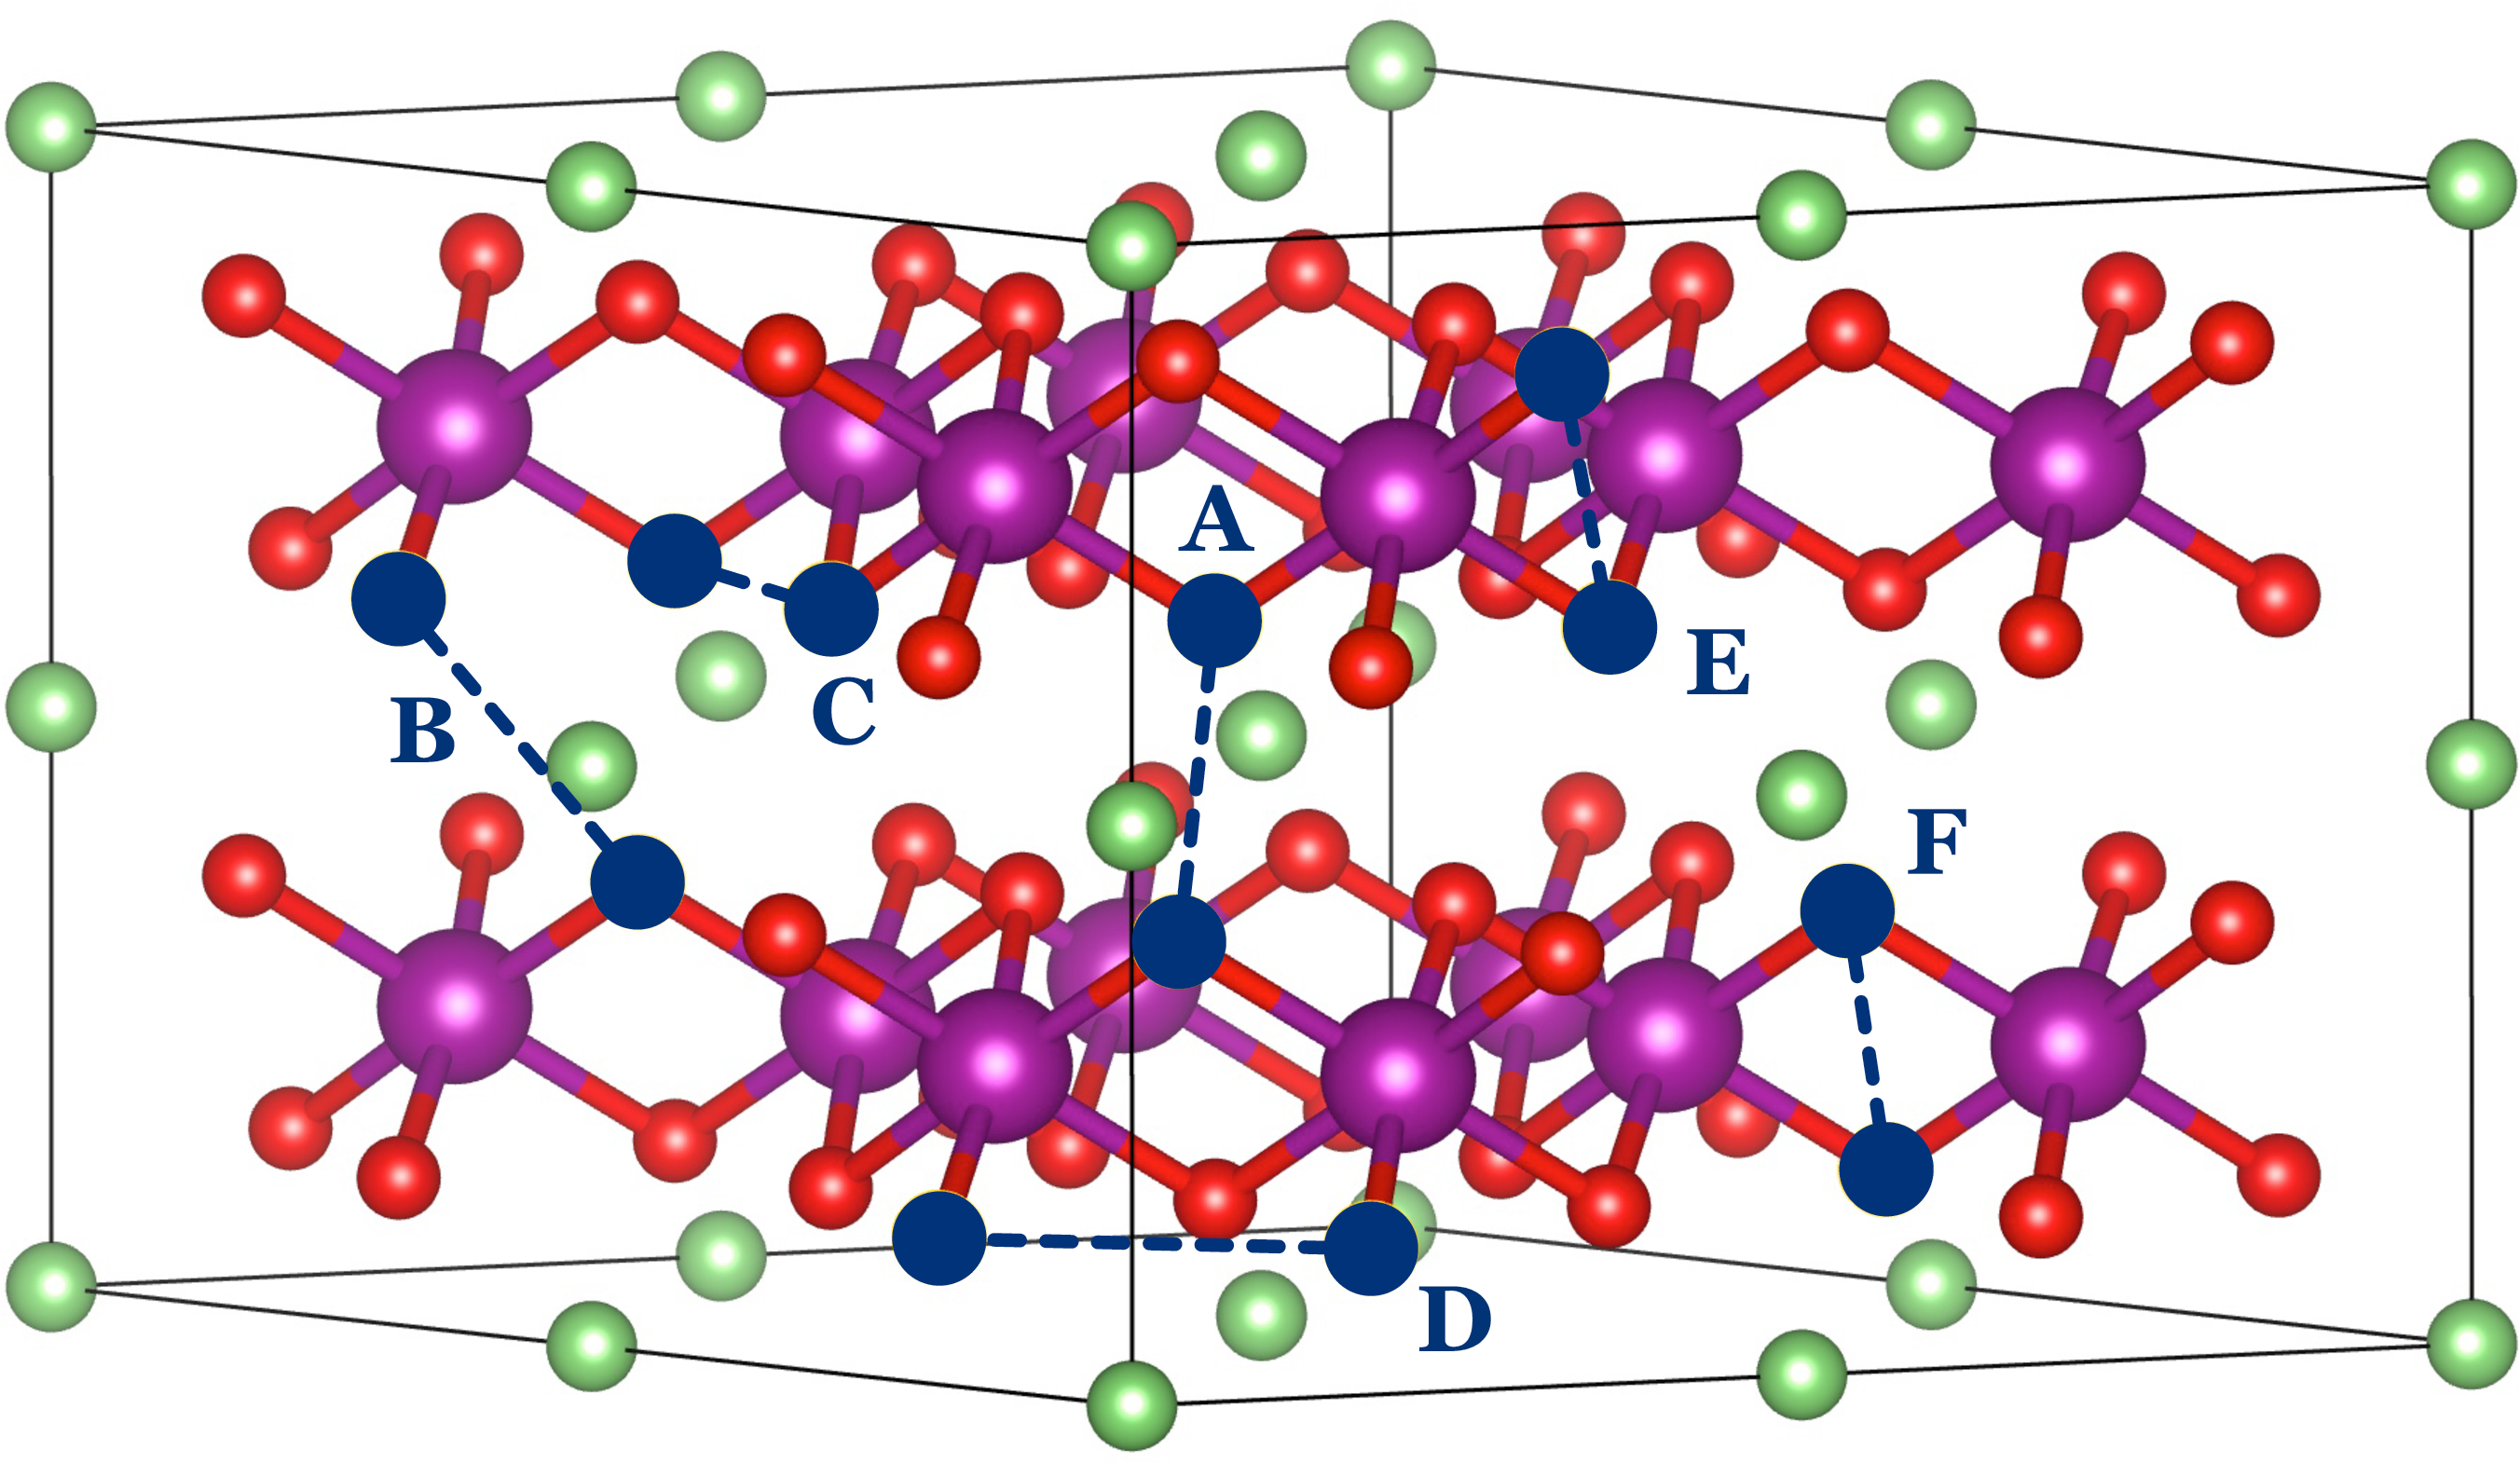
\includegraphics[width=0.6\textwidth]{Figures/batteries/oxygen_dimers.png} 
\caption{Potential oxygen dimers in O1-\ce{Li_{0.5}[Mn, Ir]O3}.} 
\label{batteries:fig-oxygen_dimers}  
\end{figure} 
 
To calculate the chemical reaction energy of the dimer formation, we construct 
a 2$\times$2$\times$2 supercell of the primitive unit cell, for the O1 stacking of 75\% 
charged \ce{Li_{0.5}MnO3} and \ce{Li_{0.5}IrO3} 
(Fig.~\ref{batteries:fig-oxygen_dimers}). In order to rigorously study the 
dimer formation, we need to consider all non-equivalent oxygen pairs that have 
the potential to form a dimer for each material. We use the workflow described 
in Section~\ref{automation:sec-dimer} to calculate the reaction energy of all
non-equivalent potential dimers in the structure. In short, all potential oxygen dimers 
in the structure are found using a voronoi decomposition to find the neighbors 
of the various atoms in the unit cell. Once all oxygen dimers have been found, 
we set up a list of all non-equivalent potential dimers based on the
symmetry operations of the structure. In the charged 
O1-\ce{Li_{0.5}MnO3} and O1-\ce{Li_{0.5}IrO3} structures, we find a total of 6 
non-equivalent dimers, shown in Fig.~\ref{batteries:fig-oxygen_dimers}. For 
each structure and each potential dimer, we reduce the distance between the 
oxygen atoms in the dimer pair to 1.4~\si{\angstrom} and once again optimize 
all atomic positions as described in the methods section. To make sure the 
interaction between the dimers in the periodic boundary conditions approach of 
\gls{VASP} is sufficiently small, we have also performed similar calculations in a 
3$\times$3$\times$3 supercell, and found the differences between the reaction energies to be 
smaller than 50~\si{\milli\electronvolt} for all potential 
dimers~\cite{Levi2020}. 
 
\begin{figure}[ht] 
\centering
\captionsetup{width=0.9\linewidth}
% 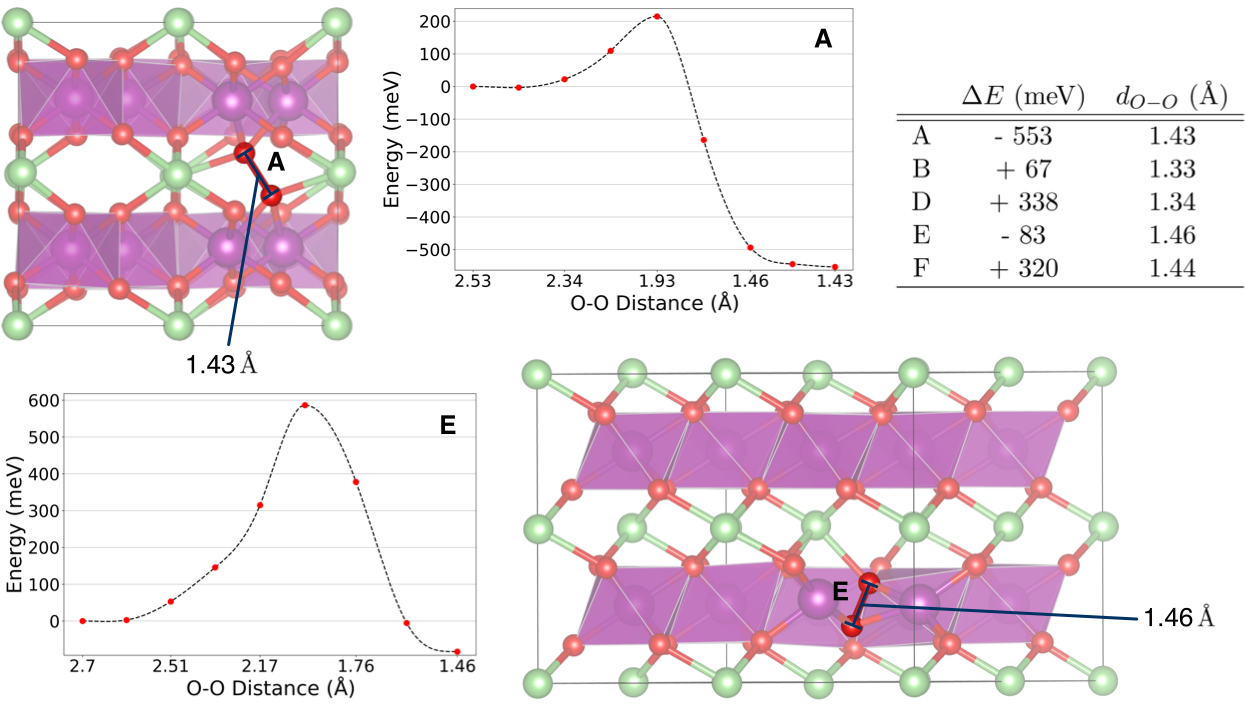
\includegraphics[width=\textwidth]{Figures/batteries/dimer_energetics.png} 
\begin{tikzpicture}[]

\node [anchor=south west] at (0, 0) {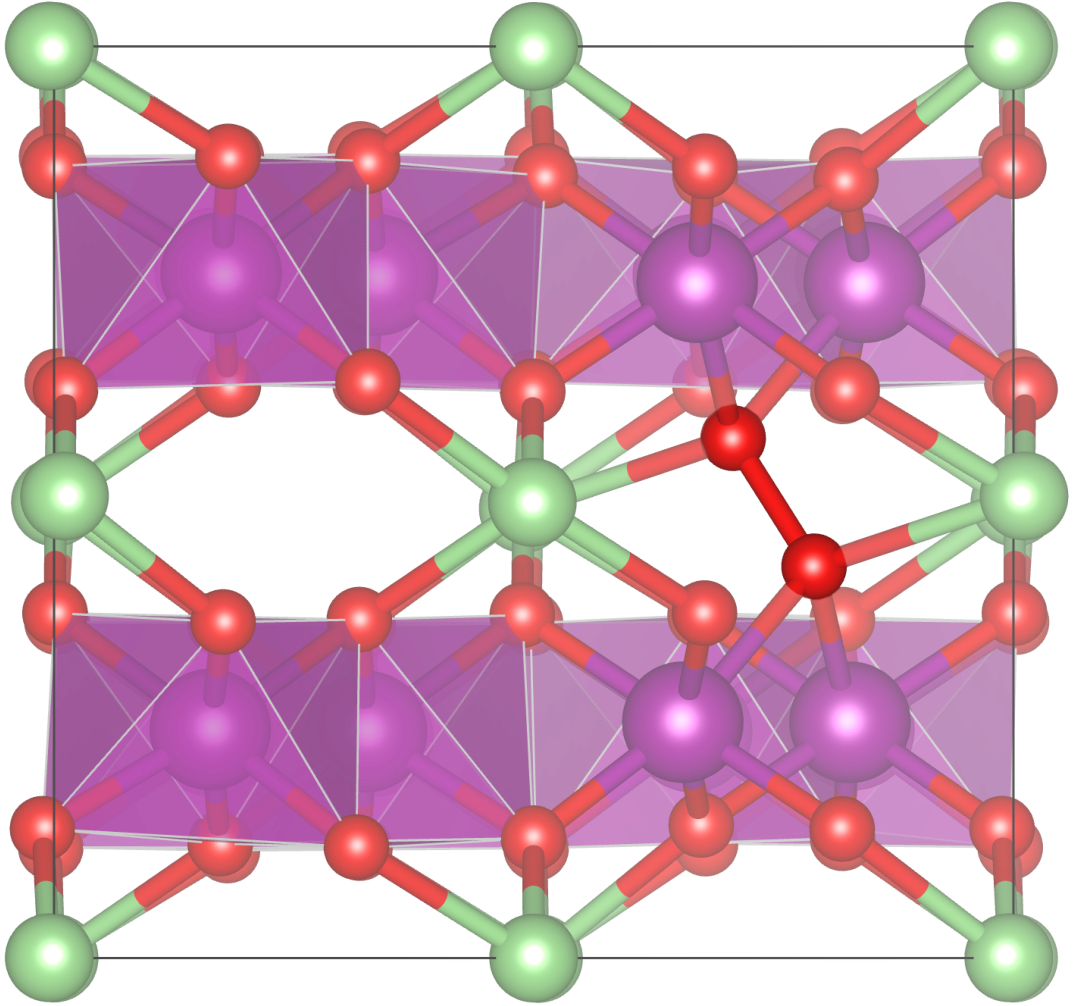
\includegraphics[height=0.3\textwidth]{\figurepath/batteries/Li2MnO3-d49_80.png}};

\coordinate (O1) at (4.01, 2.2);
\coordinate (O2) at (3.6, 2.85);
\node (distance1) [font=\small] at (6, 4.8) {1.43 \si{\angstrom}};
\draw [<->, >=|, very thick] (O1) -- (O2);
\draw [-, thick] ($(O1)!0.5!(O2)$) -- (distance1);

\begin{axis}[
height=5cm, 
width=0.4\textwidth, 
at={(0.45\textwidth, 3.3em)},
x dir=reverse,
xlabel={O-O Distance (\si{\angstrom})},
ylabel={Energy (meV)},
xticklabel={$\mathsf{\pgfmathprintnumber{\tick}}$},
yticklabel={$\mathsf{\pgfmathprintnumber{\tick}}$},
]

% This file was created by tikzplotlib v0.9.1.
\addplot [thick, black, dashed]
table {%
1.43041498524752 -553.091260000031
1.44041498524752 -551.377642628582
1.45041498524752 -546.431762921848
1.46041498524752 -538.54607949124
1.47041498524752 -528.013050948175
1.48041498524752 -515.125135904066
1.49041498524752 -500.174792970328
1.50041498524752 -483.454480758375
1.51041498524752 -465.256657879622
1.52041498524752 -445.873782945484
1.53041498524752 -425.598314567374
1.54041498524752 -404.722711356706
1.55041498524752 -383.539431924897
1.56041498524752 -362.340934883359
1.57041498524752 -341.419678843507
1.58041498524752 -321.018386344896
1.59041498524752 -301.150542620496
1.60041498524752 -281.763631502026
1.61041498524752 -262.805130781514
1.62041498524752 -244.222518250986
1.63041498524752 -225.963271702471
1.64041498524752 -207.974868927997
1.65041498524752 -190.204787719591
1.66041498524752 -172.600505869281
1.67041498524752 -155.109501169094
1.68041498524752 -137.679251411059
1.69041498524752 -120.257234387202
1.70041498524752 -102.790927889552
1.71041498524752 -85.2278097101362
1.72041498524752 -67.5153576409824
1.73041498524752 -49.6010494741182
1.74041498524752 -31.4323630015713
1.75041498524752 -12.9567760153694
1.76041498524752 5.87823369245977
1.77041498524752 25.124203929812
1.78041498524752 44.7651207939874
1.79041498524752 64.6750691859931
1.80041498524752 84.7180456287522
1.81041498524752 104.758046645188
1.82041498524752 124.659068758223
1.83041498524752 144.28510849078
1.84041498524752 163.500162365784
1.85041498524752 182.168226906156
1.86041498524752 200.153298634819
1.87041498524752 217.319374074698
1.88041498524752 233.530449748714
1.89041498524752 248.650522179791
1.90041498524752 262.543587890852
1.91041498524752 275.073643404821
1.92041498524752 286.104685244619
1.93041498524752 295.50070993317
1.94041498524752 303.125713993398
1.95041498524752 308.843693948225
1.96041498524752 312.518646320574
1.97041498524752 314.014567633369
1.98041498524752 313.398597500051
1.99041498524752 311.053533252383
2.00041498524752 307.13022917784
2.01041498524752 301.773806636548
2.02041498524752 295.129386988631
2.03041498524752 287.342091594215
2.04041498524752 278.557041813427
2.05041498524752 268.919359006392
2.06041498524752 258.574164533235
2.07041498524752 247.666579754083
2.08041498524752 236.341726029061
2.09041498524752 224.744724718295
2.10041498524752 213.020697181911
2.11041498524752 201.314764780033
2.12041498524752 189.772048872789
2.13041498524752 178.537670820304
2.14041498524752 167.756751982704
2.15041498524752 157.574413720114
2.16041498524752 148.134379241703
2.17041498524752 139.505115028043
2.18041498524752 131.643149700525
2.19041498524752 124.495913025972
2.20041498524752 118.010834771208
2.21041498524752 112.135344703057
2.22041498524752 106.816872588343
2.23041498524752 102.00284819389
2.24041498524752 97.6407012865209
2.25041498524752 93.6778616330605
2.26041498524752 90.0617590003324
2.27041498524752 86.7398231551602
2.28041498524752 83.6594838643678
2.29041498524752 80.7681708947793
2.30041498524752 78.0133140132184
2.31041498524752 75.3423429865087
2.32041498524752 72.7111848560701
2.33041498524752 70.1329170892376
2.34041498524752 67.6441771638725
2.35041498524752 65.2816761285648
2.36041498524752 63.0821250319044
2.37041498524752 61.0822349224814
2.38041498524752 59.3187168488857
2.39041498524752 57.8282818597072
2.40041498524752 56.6476410035358
2.41041498524752 55.8135053289616
2.42041498524752 55.3591156502156
2.43041498524752 55.0730147158313
2.44041498524752 54.3418496115398
2.45041498524752 52.5149106078037
2.46041498524752 48.941487975086
2.47041498524752 43.0266663682665
2.48041498524752 35.0638700443965
2.49041498524752 26.0588023425712
2.50041498524752 17.0372094540019
2.51041498524752 9.02483756989976
2.52041498524752 3.04743288147699
2.53041498524752 0.130741579945283
};
\addplot [thick, red, mark=*, mark size=2, mark options={solid}, only marks]
table {%
2.53289368015598 0
2.46457000294431 46.7890599999805
2.41729780104295 55.45982000001
2.31211857608837 74.8918900000035
2.15692701821804 151.334410000004
1.97196758439653 314.042639999968
1.76726251651896 19.0099999999802
1.57088682042962 -340.444320000017
1.43041498524752 -553.091260000031
};


\end{axis}

\node [font=\bfseries, anchor=north west] at (7.2, 4.6) {A};

\node (fig2) [anchor=south east] at (0.95\textwidth, -13em) {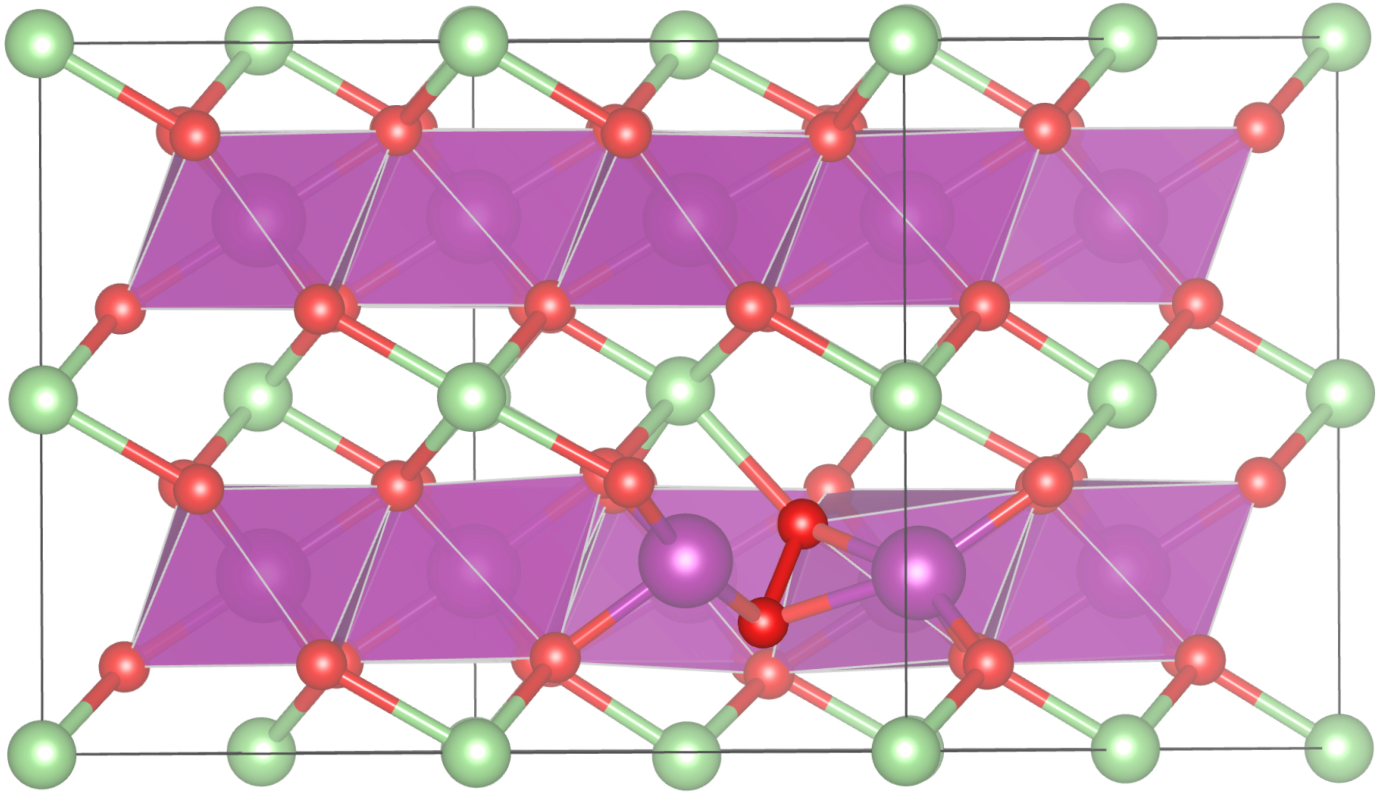
\includegraphics[height=0.3\textwidth]{\figurepath/batteries/Li2MnO3-d48_92.png}};

\coordinate (O1) at ($(fig2) + (0.705, -0.75)$);
\coordinate (O2) at ($(fig2) + (0.44, -1.39)$);
\node (distance) [
font=\small, fill=white, fill opacity=0.6, text opacity=1, rounded corners
] at (14, -3.5) {1.46 \si{\angstrom}};
\draw [<->, >=|, very thick] (O1) -- (O2);
\draw [-, thick] ($(O1)!0.5!(O2)$) -- (distance);

\begin{axis}[
height=5cm, 
width=0.4\textwidth, 
at={(0.1\textwidth, -9.7em)},
x dir=reverse,
xlabel={O-O Distance (\si{\angstrom})},
ylabel={Energy (meV)},
xticklabel={$\mathsf{\pgfmathprintnumber{\tick}}$},
yticklabel={$\mathsf{\pgfmathprintnumber{\tick}}$},
]

% This file was created by tikzplotlib v0.9.1.
\addplot [thick, black, dashed]
table {%
1.4566494053843 -82.8172899999799
1.4666494053843 -81.2560763673107
1.4766494053843 -76.7947268149007
1.4866494053843 -69.7666783611462
1.4966494053843 -60.5053680244437
1.5066494053843 -49.3442328231896
1.5166494053843 -36.6167097757802
1.5266494053843 -22.6562359006121
1.5366494053843 -7.79624821608146
1.5466494053843 7.65847202609837
1.5566494053843 23.5899600898859
1.5666494053843 39.9551223502687
1.5766494053843 56.7110651744154
1.5866494053843 73.8148949294948
1.5966494053843 91.2237179826755
1.6066494053843 108.894640701126
1.6166494053843 126.784769452016
1.6266494053843 144.851210602513
1.6366494053843 163.051070519786
1.6466494053843 181.341455571004
1.6566494053843 199.679472123335
1.6666494053843 218.022226543949
1.6766494053843 236.326825200013
1.6866494053843 254.550374458698
1.6966494053843 272.64998068717
1.7066494053843 290.5827502526
1.7166494053843 308.305789522155
1.7266494053843 325.776204863005
1.7366494053843 342.951102642318
1.7466494053843 359.787589227262
1.7566494053843 376.242770985008
1.7666494053843 392.275847347668
1.7766494053843 407.857689302546
1.7866494053843 422.96321199675
1.7966494053843 437.567334526386
1.8066494053843 451.644975987557
1.8166494053843 465.171055476366
1.8266494053843 478.120492088916
1.8366494053843 490.468204921312
1.8466494053843 502.189113069657
1.8566494053843 513.258135630055
1.8666494053843 523.650191698609
1.8766494053843 533.340200371423
1.8866494053843 542.303080744601
1.8966494053843 550.513751914245
1.9066494053843 557.947132976461
1.9166494053843 564.57814302735
1.9266494053843 570.381701163017
1.9366494053843 575.332726479567
1.9466494053843 579.406138073101
1.9566494053843 582.576855039724
1.9666494053843 584.819796475539
1.9766494053843 586.10988147665
1.9866494053843 586.390403545011
1.9966494053843 584.489733791969
2.0066494053843 579.980430115906
2.0166494053843 573.074663703546
2.0266494053843 563.984605741615
2.0366494053843 552.922427416838
2.0466494053843 540.100299915941
2.0566494053843 525.730394425649
2.0666494053843 510.024882132686
2.0766494053843 493.195934223779
2.0866494053843 475.455721885652
2.0966494053843 457.016416305032
2.1066494053843 438.090188668641
2.1166494053843 418.889210163206
2.1266494053843 399.625651975454
2.1366494053843 380.511685292108
2.1466494053843 361.759481299893
2.1566494053843 343.581211185535
2.1666494053843 326.189046135761
2.1766494053843 309.793704112122
2.1866494053843 294.506612795319
2.1966494053843 280.277909230181
2.2066494053843 267.042954730596
2.2166494053843 254.73711061045
2.2266494053843 243.295738183629
2.2366494053843 232.654198764022
2.2466494053843 222.747853665516
2.2566494053843 213.512064201998
2.2666494053843 204.882191687355
2.2766494053843 196.793597435474
2.2866494053843 189.181642760244
2.2966494053843 181.981688975551
2.3066494053843 175.129097395282
2.3166494053843 168.559229333324
2.3266494053843 162.207446103566
2.3366494053843 156.009109019893
2.3466494053843 149.899579396194
2.3566494053843 143.814517236325
2.3666494053843 137.714015193111
2.3766494053843 131.600347923166
2.3866494053843 125.479973967742
2.3966494053843 119.359351868087
2.4066494053843 113.244940165453
2.4166494053843 107.143197401088
2.4266494053843 101.060582116243
2.4366494053843 95.0035528521679
2.4466494053843 88.9785681501126
2.4566494053843 82.9920865513269
2.4666494053843 77.0505665970607
2.4766494053843 71.160466828564
2.4866494053843 65.3282457870872
2.4966494053843 59.56036201388
2.5066494053843 53.863274050192
2.5166494053843 48.2467496563142
2.5266494053843 42.7433675729223
2.5366494053843 37.3953200687798
2.5466494053843 32.2448331135497
2.5566494053843 27.3341326768954
2.5666494053843 22.7054447284804
2.5766494053843 18.4009952379677
2.5866494053843 14.4630101750202
2.5966494053843 10.9337155093015
2.6066494053843 7.85533721047477
2.6166494053843 5.27010124820321
2.6266494053843 3.22023359214989
2.6366494053843 1.73915479787467
2.6466494053843 0.772752158584978
2.6566494053843 0.216767002869623
2.6666494053843 -0.0336518700062289
2.6766494053843 -0.0833556607773805
2.6866494053843 -0.0371955701786719
};
\addplot [thick, red, mark=*, mark size=2, mark options={solid}, only marks]
table {%
2.69644801919029 0
2.62954078608243 2.73332000000437
2.50843083366394 52.8562999999735
2.35371734388973 145.599790000006
2.17349124489821 314.85189
1.98479888323523 586.43914999999
1.7577491767086 378.027349999968
1.53825382424304 -5.35070000000815
1.4566494053843 -82.8172899999799
};


\end{axis}
\node [font=\bfseries, anchor=north west] at (1.65, -0.4) {E};


\node [anchor=south east] at (0.95\textwidth, 3em) {%
\begin{tabular}{lr}
\multicolumn{2}{c}{$\Delta E$ (meV)} \\\hline
\textbf{A} & -553 \\
\textbf{B} & +67 \\
\textbf{C} & $\rightarrow$ \textbf{A} \\
\textbf{D} & +338 \\
\textbf{E} & -83 \\
\textbf{F} & +320 \\
\hline
\end{tabular}
};

\end{tikzpicture}

\caption{Reaction energies $\Delta E$, final O-O bond length $d_{O-O}$ and 
kinetic barriers for the dimers in O1-\ce{Li_{0.5}MnO3}. The final geometry 
and kinetic barrier is only shown for dimer \textbf{A} and \textbf{E}, which 
have a negative reaction energy.} 
\label{batteries:fig-Mn_dimers} 
\end{figure} 
 
Figure~\ref{batteries:fig-Mn_dimers} shows the results for the reaction energy 
and final bond length. Even though all perturbed structures 
produce a stable oxygen dimer after optimization, only two dimers have a 
negative reaction energy, which are labeled as \textbf{A} and \textbf{E} 
in Fig.~\ref{batteries:fig-oxygen_dimers}. One dimer (\textbf{C}) results in a 
geometry similar to the formation of the \textbf{E} dimer, with comparable 
energies. The two dimers that have a reduced energy in the final state are 
formed by two oxygen atoms from different layers, with dimer \textbf{A} being 
the most energetically favorable by far. The final structures of both 
dimers are shown in Fig.~\ref{batteries:fig-Mn_dimers}, along with the kinetic barrier, 
calculated using the \gls{NEB} method. For the \textbf{A} dimer, the kinetic barrier 
is equal to 314~\si{\milli\electronvolt}, which is smaller than the typical 
kinetic barrier for lithium migration in layered 
structures~\cite{VanDerVen2013}. This implies that the formation of the 
\textbf{A} dimer is very likely to occur during the charging process. The 
kinetic barrier for the \textbf{E} dimer is significantly higher at 
586~\si{\milli\electronvolt}, but is by no means insurmountable. Hence, we 
would expect to find both dimers to play a significant role in the structural 
changes that occur for \ce{Li2MnO3} as it is cycled. 
 
In stark contrast with the results of O1-\ce{Li_{0.5}MnO3}, none of the dimer 
optimizations for O1-\ce{Li_{0.5}IrO3} result in a new geometry with a lower 
energy as the unperturbed structure. In fact, out of all the dimers, all but 
one return to the original oxygen framework. The only dimer that is stable 
after optimization has an increased energy of +2.2~\si{\electronvolt}, and is 
hence unlikely to ever be formed in practice. In our view, the enhanced 
stability of the oxygen framework can be in part explained by the reduced 
participation of oxygen in the redox process as the battery is charged, which 
is believed to be the primary driver for dimer formation. 
 
\section{Substitutions} \label{batteries:sec-substitutions} 
 
Based on the discussion from Section~\ref{batteries:sec-lirich}, it is clear 
that the stability of the oxygen lattice plays an important role in 
maintaining the structure of Li-rich cathodes as the battery is cycled. One 
suggested strategy for stabilizing the oxygen framework is the (partial) 
substitution of \ce{Mn^{4+}} by other elements. Based on our results, as well 
as the results of McCalla et al.~\cite{McCalla2015}, \ce{Ir^{4+}} seems like a 
natural choice, as this leads to an improved stability of the structure and 
hence better cycling properties. However, designing a \ce{Ir}-based cathode 
material is not a practical approach due to the weight and price of \ce{Ir}. 
 
Another element that has been suggested in order to improve the cycling 
behavior of Li-rich materials is \ce{Sn^{4+}}, for several reasons. First, 
the bonding energy of \ce{Sn-O} is higher than that of \ce{Mn-O}, which can 
enhance the structural stability~\cite{Qiao2015}. Second, \ce{Sn^{4+}} does 
not tend to adopt a tetrahedral coordination~\cite{Sathiya2013} and has a much 
larger ionic radius compared to \ce{Mn^{4+}}, implying that the migration of 
\ce{Sn^{4+}} to the \ce{Li} layers is less likely to occur as the battery is 
charged\footnote{Note that the migration path for \ce{Sn^{4+}} does not have 
to pass a tetrahedral site in case the stacking is changed from O3 to O1.}. 
For these reasons, \ce{Sn^{4+}} was chosen as the first element by our 
experimental collaborators from Hasselt University\footnote{Andreas Paulus, 
Marlies van Bael and An Hardy, \href{https://www.uhasselt.be/UH/IMO/Visit-the-groups/Inorganic-and-physical-chemistry-(IPC).html}{Inorganic and Physical Chemistry}, Hasselt University.} to substitute in 
Li-rich \gls{NMC} samples in an attempt to improve the cycling properties of the 
cathode. 

In this section, I start by briefly discussing their powder X-ray diffraction (\gls{PXRD}) results, as well as 
the energy-dispersive X-ray analysis (\gls{EDX}) results of our collaborators within EMAT\footnote{Myl\`ene Hendrickx, Olesia 
Karakulina, Artem Abakumov and Joke Hadermann, \href{https://www.uantwerpen.be/en/research-groups/emat/}{Electron Microscopy for Materials 
Science}, Antwerp University.}, as a motivation for the 
calculations we have performed on the solubility of \ce{Sn} in a 
Li-rich/Mn-rich material. Next, I perform a similar analysis as in the 
previous section for investigating the influence of Sn-substitution on the 
stability of the oxygen framework. Finally, I extend this analysis to the 
substitution of several other elements that have the potential to oxidize 
further (\ce{Co}, \ce{V} and \ce{Mo}), in order to investigate if they have a 
stabilizing effect similar to that of \ce{Ir}.  

\resultsubsection{Thermodynamic Stability of Sn substitution \label{batteries:sec-Sn_stability}}{https://github.com/mbercx/phd-thesis/tree/master/jupyter/batteries/README.md\#thermodynamic-stability-of-sn-substitution}{sn_stability}
 
Although the increased ionic radius of \ce{Sn^{4+}} compared to \ce{Mn^{4+}} 
is believed to inhibit its migration into the Li-layer, it can potentially 
also lead to a reduced solubility of \ce{Sn} in the \gls{NMC} structure. In order to 
investigate the solubility of Sn in Li-rich \gls{NMC}, several samples with 
increased Sn-substitution were prepared for a Li-rich/Mn-rich \gls{NMC} structure, 
leading to stoichiometries \ce{Li_{1.2}Ni_{0.13}Co_{0.13}Mn_{0.54-x}Sn_xO2} 
for $x  \approx 0, 0.027, 0.054, 0.108 \textrm{ and } 0.54$. Looking at the 
change in the \gls{PXRD} pattern of Sn-substituted \gls{NMC} samples in 
Fig.~\ref{batteries:fig-Sn_experiment}a, a second phase appears as the 
amount of Sn is increased, starting from $x = 0.054$. This phase becomes dominant for $x=0.54$ and was 
identified as \ce{Li2SnO3} based on an indexation of the \gls{PXRD} results. 
The \gls{EDX} results for a particle with $x=0.108$ 
(Fig.~\ref{batteries:fig-Sn_experiment}b) indicate that the exsolution of this 
Sn-rich phase already occurs at lower levels of Sn-substitution. 
 
\begin{figure}[ht] 
    \centering
    \captionsetup{width=0.92\linewidth}
    \begin{tikzpicture}

\definecolor{Sn}{HTML}{FE31FD}
\definecolor{Mn}{HTML}{12DC1F}

\node [font=\bfseries, anchor=south] at (0.03\textwidth, -1.5em) {a};

\begin{axis}[
anchor=north west,
at={(0.05\textwidth, 0)},
width=0.6\textwidth, height=6cm,
xlabel={2$\theta$(\si{\degree})},
xmin=5.0, xmax=80.0,
ylabel={Intensity (a.u.)},
ytick={}, yticklabels={}
]
% This file was created by tikzplotlib v0.9.1.
\definecolor{color0}{rgb}{0.0862745098039216,0.23921568627451,0.36078431372549}
\definecolor{color1}{rgb}{0.694117647058824,0.8,0.890196078431372}
\definecolor{color2}{rgb}{0.227450980392157,0.662745098039216,0.623529411764706}
\definecolor{color3}{rgb}{0.933333333333333,0.811764705882353,0.352941176470588}
\definecolor{color4}{rgb}{0.901960784313726,0.32156862745098,0.223529411764706}

\addplot [semithick, color0]
table {%
4.0025 -0.00138
4.0525 0.00134
4.1025 0.00223
4.1525 0.00082
4.2025 0.004
4.2525 0.00408
4.3025 0.00419
4.3525 0.00292
4.4025 0.00346
4.4525 0.0026
4.5025 0.00527
4.5525 0.00271
4.6025 0.00336
4.6525 0.00363
4.7025 0.00327
4.7525 0.00225
4.8025 0.0053
4.8525 0.00086
4.9025 0.00456
4.9525 0.00369
5.0025 0.00226
5.0525 0.00273
5.1025 0.00319
5.1525 0.00312
5.2025 0.00416
5.2525 0.00294
5.3025 0.00377
5.3525 0.00382
5.4025 0.00198
5.4525 0.00232
5.5025 0.0026
5.5525 0.00268
5.6025 0.00389
5.6525 0.00095
5.7025 0.0025
5.7525 0.00173
5.8025 0.00259
5.8525 0.00159
5.9025 0.00131
5.9525 0.00315
6.0025 0.00211
6.0525 0.00196
6.1025 0.00229
6.1525 0.00217
6.2025 0.00244
6.2525 0.00427
6.3025 0.00297
6.3525 0.00224
6.4025 0.00172
6.4525 0.00154
6.5025 0.00216
6.5525 0.00035
6.6025 0.00074
6.6525 0.00133
6.7025 0.00213
6.7525 0.00197
6.8025 0.00271
6.8525 0.00148
6.9025 0.0008
6.9525 0.002
7.0025 0.00074
7.0525 0.00141
7.1025 0.0006
7.1525 -0.00013
7.2025 0.00108
7.2525 -0.0013
7.3025 0.00033
7.3525 0.00068
7.4025 0.00025
7.4525 0.0001
7.5025 0.00025
7.5525 0.00064
7.6025 -0.00066
7.6525 -0.00099
7.7025 0.00101
7.7525 -0.00022
7.8025 0.0005
7.8525 0.0017
7.9025 -0.00129
7.9525 -0.00054
8.0025 0.00073
8.0525 -0.00059
8.1025 0.00137
8.1525 0.00018
8.2025 0.00215
8.2525 0.00052
8.3025 0.00041
8.3525 0.00125
8.4025 -4e-05
8.4525 0.00074
8.5025 0.00052
8.5525 -0.00052
8.6025 0.00092
8.6525 -0.00062
8.7025 -0.00024
8.7525 0.00137
8.8025 0.00086
8.8525 0.00017
8.9025 0.00082
8.9525 0.00106
9.0025 0.00114
9.0525 -0.00112
9.1025 0.00063
9.1525 0.00066
9.2025 0.00106
9.2525 0.0015
9.3025 0.00053
9.3525 -0.00097
9.4025 0.00219
9.4525 0.00045
9.5025 -0.0001
9.5525 -0.00035
9.6025 0.00066
9.6525 0.0008
9.7025 0.00081
9.7525 0.00121
9.8025 0.00235
9.8525 0.00051
9.9025 0.00061
9.9525 0.00192
10.0025 0.00111
10.0525 0.00029
10.1025 -0.00053
10.1525 -0.00041
10.2025 0.00045
10.2525 -0.00041
10.3025 0.00035
10.3525 0.00048
10.4025 -0.00125
10.4525 0.00057
10.5025 0.00115
10.5525 0.00148
10.6025 0.00057
10.6525 0.00101
10.7025 -0.00023
10.7525 0
10.8025 0.00051
10.8525 0.00279
10.9025 0.00115
10.9525 0.00071
11.0025 0.00027
11.0525 -0.00038
11.1025 0.00049
11.1525 0.00165
11.2025 0.0021
11.2525 0.00114
11.3025 0.00061
11.3525 -0.00027
11.4025 0.00017
11.4525 3e-05
11.5025 0.00162
11.5525 0.00063
11.6025 0.00135
11.6525 -0.00039
11.7025 0.00059
11.7525 0.00104
11.8025 0.00159
11.8525 0.00047
11.9025 0.00205
11.9525 0.00105
12.0025 0.00142
12.0525 0.00069
12.1025 0.00175
12.1525 0.00107
12.2025 0.00078
12.2525 -3e-05
12.3025 0.00091
12.3525 0.00133
12.4025 0.00227
12.4525 0.00217
12.5025 0.00256
12.5525 0.0004
12.6025 0.00181
12.6525 0.0012
12.7025 0.00079
12.7525 0.00039
12.8025 0.00266
12.8525 0.00045
12.9025 0.0016
12.9525 -0.00051
13.0025 0.00135
13.0525 0.00226
13.1025 0.0015
13.1525 0.00198
13.2025 0.00121
13.2525 0.00211
13.3025 0.00217
13.3525 0.00109
13.4025 0.00139
13.4525 -5e-05
13.5025 0.00111
13.5525 0.0014
13.6025 0.00015
13.6525 0.00177
13.7025 0.00167
13.7525 0.0003
13.8025 0.00157
13.8525 9e-05
13.9025 0.00194
13.9525 0.0013
14.0025 0.00165
14.0525 -0.00103
14.1025 0.00063
14.1525 0.00051
14.2025 0.00106
14.2525 0.00043
14.3025 0.00052
14.3525 0.00059
14.4025 0.0004
14.4525 0.00114
14.5025 0.00085
14.5525 0.0009
14.6025 0.00071
14.6525 0.0001
14.7025 0.0004
14.7525 -0.00089
14.8025 0.0022
14.8525 0.00104
14.9025 0.00152
14.9525 0.00166
15.0025 0.0014
15.0525 0.00084
15.1025 0.00049
15.1525 0.00043
15.2025 0.0008
15.2525 -0.00112
15.3025 0.00035
15.3525 0.00133
15.4025 0.00082
15.4525 0.00039
15.5025 0.00016
15.5525 0.00073
15.6025 0.00294
15.6525 0.00061
15.7025 0.00129
15.7525 7e-05
15.8025 0.0009
15.8525 0.00027
15.9025 0.00049
15.9525 0.00046
16.0025 0.00106
16.0525 0.00061
16.1025 0.00046
16.1525 0.00104
16.2025 0.0016
16.2525 0.00215
16.3025 0.00048
16.3525 0.00086
16.4025 0.00307
16.4525 0.00119
16.5025 0.00208
16.5525 0.00016
16.6025 0.00128
16.6525 0.00038
16.7025 0.00147
16.7525 -3e-05
16.8025 0.00172
16.8525 0.00172
16.9025 0.00157
16.9525 0.00113
17.0025 -0.00065
17.0525 0.00039
17.1025 0.00248
17.1525 0.00236
17.2025 0.00252
17.2525 0.00207
17.3025 0.00194
17.3525 0.00215
17.4025 0.00467
17.4525 0.00263
17.5025 0.00397
17.5525 0.00431
17.6025 0.00324
17.6525 0.00293
17.7025 0.00487
17.7525 0.00209
17.8025 0.00401
17.8525 0.0057
17.9025 0.0058
17.9525 0.00633
18.0025 0.00761
18.0525 0.01082
18.1025 0.01491
18.1525 0.0181
18.2025 0.02695
18.2525 0.03626
18.3025 0.04883
18.3525 0.06335
18.4025 0.08724
18.4525 0.11599
18.5025 0.16394
18.5525 0.23466
18.6025 0.36248
18.6525 0.51646
18.7025 0.3348
18.7525 0.09801
18.8025 0.03523
18.8525 0.01588
18.9025 0.01067
18.9525 0.00562
19.0025 0.00528
19.0525 0.00398
19.1025 0.00259
19.1525 0.00186
19.2025 0.00132
19.2525 0.00094
19.3025 0.00027
19.3525 0.00121
19.4025 0.00051
19.4525 0.00027
19.5025 7e-05
19.5525 -0.00058
19.6025 -0.00041
19.6525 -0.00018
19.7025 -0.00014
19.7525 -0.00041
19.8025 -9e-05
19.8525 -0.00097
19.9025 -0.00051
19.9525 0.00018
20.0025 0.00078
20.0525 -9e-05
20.1025 0.00057
20.1525 1e-05
20.2025 0.00012
20.2525 0.00064
20.3025 0.00154
20.3525 0.00217
20.4025 0.00364
20.4525 0.00355
20.5025 0.00543
20.5525 0.0092
20.6025 0.0122
20.6525 0.01785
20.7025 0.02075
20.7525 0.02188
20.8025 0.01694
20.8525 0.01253
20.9025 0.0108
20.9525 0.009
21.0025 0.0081
21.0525 0.00756
21.1025 0.00768
21.1525 0.00838
21.2025 0.0099
21.2525 0.00953
21.3025 0.01189
21.3525 0.01078
21.4025 0.0082
21.4525 0.00869
21.5025 0.00832
21.5525 0.00881
21.6025 0.00981
21.6525 0.00966
21.7025 0.00972
21.7525 0.00905
21.8025 0.00736
21.8525 0.00679
21.9025 0.00575
21.9525 0.00371
22.0025 0.0059
22.0525 0.00315
22.1025 0.00271
22.1525 0.00165
22.2025 0.00053
22.2525 0.00039
22.3025 0.001
22.3525 0.00151
22.4025 0.00208
22.4525 0.00089
22.5025 0.00132
22.5525 0.00011
22.6025 0.00064
22.6525 -0.00016
22.7025 0.00065
22.7525 0.0004
22.8025 0.00069
22.8525 -0.00079
22.9025 -0.00087
22.9525 0.00059
23.0025 -2e-05
23.0525 0.00035
23.1025 0.00086
23.1525 0.0011
23.2025 0.00023
23.2525 -0.00049
23.3025 -8e-05
23.3525 -0.00049
23.4025 0.00127
23.4525 0.00132
23.5025 -0.00057
23.5525 0.00087
23.6025 0.00191
23.6525 0.0013
23.7025 0.00182
23.7525 0.00227
23.8025 0.00199
23.8525 0.00168
23.9025 0.00297
23.9525 0.00121
24.0025 0.00096
24.0525 0.00237
24.1025 0.00206
24.1525 0.00324
24.2025 0.00278
24.2525 0.00264
24.3025 0.00335
24.3525 0.00352
24.4025 0.00211
24.4525 0.00081
24.5025 0.00096
24.5525 -1e-05
24.6025 -0.00044
24.6525 -0.00033
24.7025 0.00022
24.7525 -0.00073
24.8025 0.00069
24.8525 4e-05
24.9025 -0.00017
24.9525 0.0006
25.0025 0.00055
25.0525 0.00109
25.1025 0.00122
25.1525 0.00128
25.2025 0.00128
25.2525 0.00041
25.3025 -0.00112
25.3525 -0.00052
25.4025 0.00052
25.4525 0.00019
25.5025 0.00186
25.5525 -0.00012
25.6025 0.00061
25.6525 0.00089
25.7025 0.00089
25.7525 0.00064
25.8025 0.00031
25.8525 0.00089
25.9025 -0.00043
25.9525 0.00072
26.0025 0.0006
26.0525 -0.00036
26.1025 0.00092
26.1525 0.00053
26.2025 0.00121
26.2525 0.00173
26.3025 0.00081
26.3525 0.0003
26.4025 -0.00025
26.4525 9e-05
26.5025 0.0001
26.5525 0.00015
26.6025 0.00128
26.6525 0.00067
26.7025 -0.00075
26.7525 0.00174
26.8025 0.00237
26.8525 0.00087
26.9025 0.00142
26.9525 0.00208
27.0025 0.00024
27.0525 0.00106
27.1025 0.00132
27.1525 0.00115
27.2025 -0.00043
27.2525 0.00132
27.3025 0.00183
27.3525 0.00023
27.4025 0.00121
27.4525 0.0012
27.5025 0.00245
27.5525 0.00138
27.6025 0.00189
27.6525 0.00248
27.7025 0.00178
27.7525 0.00098
27.8025 0.00011
27.8525 0.00139
27.9025 0.00242
27.9525 0.0012
28.0025 0.00269
28.0525 0.00188
28.1025 0.00214
28.1525 0.00107
28.2025 0.00146
28.2525 0.00137
28.3025 0.0019
28.3525 0.00179
28.4025 0.00115
28.4525 0.00051
28.5025 0.00156
28.5525 0.00016
28.6025 0.00109
28.6525 0.0018
28.7025 0.00165
28.7525 0.00029
28.8025 0.00043
28.8525 -0.00115
28.9025 2e-05
28.9525 0.00012
29.0025 0.00058
29.0525 0.00164
29.1025 -5e-05
29.1525 -0.00027
29.2025 0.00132
29.2525 0.00106
29.3025 0.00096
29.3525 0.00021
29.4025 0.00157
29.4525 0.00228
29.5025 0.00089
29.5525 0.00152
29.6025 -0.0001
29.6525 -0.00032
29.7025 -0.00115
29.7525 -0.00031
29.8025 0.00076
29.8525 0.00092
29.9025 -0.00075
29.9525 0.00197
30.0025 -0.00031
30.0525 4e-05
30.1025 -0.00047
30.1525 0.00077
30.2025 7e-05
30.2525 0.00233
30.3025 0.00151
30.3525 0.00246
30.4025 0.00303
30.4525 0.00294
30.5025 0.0033
30.5525 0.00142
30.6025 0.00203
30.6525 0.0017
30.7025 0.00134
30.7525 0.0009
30.8025 0.00098
30.8525 0.00123
30.9025 0.0001
30.9525 0.00043
31.0025 0.00031
31.0525 0.00136
31.1025 0.00057
31.1525 0.00069
31.2025 0.00136
31.2525 0.00126
31.3025 0.00081
31.3525 0.00012
31.4025 0.0005
31.4525 -0.00013
31.5025 0.00113
31.5525 0.00118
31.6025 0.00161
31.6525 0.00327
31.7025 0.00338
31.7525 0.0043
31.8025 0.00372
31.8525 0.00269
31.9025 0.00118
31.9525 -0.00102
32.0025 0.0008
32.0525 0
32.1025 0.00046
32.1525 0.0007
32.2025 0.00177
32.2525 0.00013
32.3025 0.00079
32.3525 0.00016
32.4025 0.00216
32.4525 -0.00061
32.5025 0.00064
32.5525 0.00028
32.6025 3e-05
32.6525 -0.00014
32.7025 0.00134
32.7525 0.00154
32.8025 0.00108
32.8525 9e-05
32.9025 -0.00029
32.9525 -0.00045
33.0025 0.0018
33.0525 0.00046
33.1025 0.00075
33.1525 0.00043
33.2025 0.00116
33.2525 0.00022
33.3025 0.00061
33.3525 4e-05
33.4025 0.00039
33.4525 -0.00025
33.5025 -8e-05
33.5525 0.00044
33.6025 0.00138
33.6525 -0.00037
33.7025 0.00089
33.7525 -0.00081
33.8025 0.00179
33.8525 0.00083
33.9025 0.00158
33.9525 0.00147
34.0025 0.00145
34.0525 0.00083
34.1025 0.00122
34.1525 -0.00048
34.2025 0.00035
34.2525 5e-05
34.3025 0.00037
34.3525 0.00115
34.4025 0.0001
34.4525 0.00035
34.5025 -0.00062
34.5525 -4e-05
34.6025 0.00039
34.6525 5e-05
34.7025 0.00011
34.7525 0.00064
34.8025 0.00121
34.8525 0.00039
34.9025 0.00048
34.9525 0.00103
35.0025 0.00214
35.0525 -0.00031
35.1025 0.00128
35.1525 6e-05
35.2025 4e-05
35.2525 -0.00048
35.3025 -0.00047
35.3525 -0.00112
35.4025 -0.00019
35.4525 -0.00112
35.5025 -0.00056
35.5525 0.00075
35.6025 0.00066
35.6525 0.00027
35.7025 -0.00012
35.7525 -0.00029
35.8025 -0.00042
35.8525 -0.00038
35.9025 -0.00018
35.9525 -0.00092
36.0025 -1e-05
36.0525 0.00021
36.1025 0.00163
36.1525 0.00021
36.2025 0.00011
36.2525 0.0008
36.3025 -0.00027
36.3525 0.0008
36.4025 0.001
36.4525 0.0013
36.5025 0.00293
36.5525 0.00355
36.6025 0.0075
36.6525 0.01186
36.7025 0.02364
36.7525 0.04546
36.8025 0.08981
36.8525 0.1494
36.9025 0.18153
36.9525 0.1054
37.0025 0.04245
37.0525 0.01726
37.1025 0.01004
37.1525 0.00497
37.2025 0.00299
37.2525 0.00201
37.3025 0.00184
37.3525 0.00117
37.4025 0.00184
37.4525 0.0017
37.5025 0.00107
37.5525 0.00102
37.6025 0.00179
37.6525 0.00083
37.7025 0.00197
37.7525 0.00308
37.8025 0.00846
37.8525 0.01141
37.9025 0.01384
37.9525 0.00694
38.0025 0.00216
38.0525 0.00207
38.1025 0.00233
38.1525 0.00259
38.2025 0.00132
38.2525 0.00154
38.3025 0.00249
38.3525 0.00368
38.4025 0.00972
38.4525 0.01707
38.5025 0.02998
38.5525 0.03399
38.6025 0.01841
38.6525 0.00717
38.7025 0.00547
38.7525 0.0024
38.8025 0.0019
38.8525 0.00111
38.9025 0.0021
38.9525 0.00107
39.0025 0.00185
39.0525 -0.00039
39.1025 0.00106
39.1525 0.00022
39.2025 0.00175
39.2525 0.00045
39.3025 0.00056
39.3525 0.00158
39.4025 0.00187
39.4525 0.00034
39.5025 0.00109
39.5525 0.00217
39.6025 0.0005
39.6525 0.00184
39.7025 0.00114
39.7525 -0.00018
39.8025 0.00097
39.8525 0.00127
39.9025 0.00153
39.9525 0.00113
40.0025 0.00098
40.0525 -0.00113
40.1025 -0.00064
40.1525 0.00021
40.2025 -0.00014
40.2525 0.00061
40.3025 -0.00028
40.3525 0.00038
40.4025 0.00098
40.4525 -0.00022
40.5025 -9e-05
40.5525 0.00182
40.6025 0.00174
40.6525 0.00093
40.7025 -0.00056
40.7525 -9e-05
40.8025 0.00191
40.8525 -0.00036
40.9025 0.00031
40.9525 0.00046
41.0025 0.00026
41.0525 -6e-05
41.1025 0.00169
41.1525 0.0018
41.2025 0.00225
41.2525 0.0014
41.3025 0.00061
41.3525 0.00023
41.4025 0.00037
41.4525 0.00111
41.5025 0.00048
41.5525 -0.00111
41.6025 0.00039
41.6525 0.00068
41.7025 -0.00027
41.7525 0.00178
41.8025 0.00049
41.8525 0.0001
41.9025 0.00069
41.9525 -0.00039
42.0025 0.00216
42.0525 0.00027
42.1025 0.00191
42.1525 0.00041
42.2025 0.00088
42.2525 0.00068
42.3025 0.00062
42.3525 0.00068
42.4025 0.00257
42.4525 0.00078
42.5025 0.00088
42.5525 0.00131
42.6025 0.00091
42.6525 0.00099
42.7025 0.00107
42.7525 0.00015
42.8025 0.00176
42.8525 0.00084
42.9025 0.00052
42.9525 -0.00037
43.0025 0.00195
43.0525 0.00094
43.1025 0.00137
43.1525 0.00089
43.2025 0.00067
43.2525 0.00039
43.3025 -0.00101
43.3525 0.00056
43.4025 0.00082
43.4525 0.00121
43.5025 0.00063
43.5525 0.00131
43.6025 0.00308
43.6525 0.00256
43.7025 0.00131
43.7525 0.00198
43.8025 0.00147
43.8525 0.0016
43.9025 0.00155
43.9525 0.00188
44.0025 0.00347
44.0525 0.00417
44.1025 0.00433
44.1525 0.0054
44.2025 0.00909
44.2525 0.01106
44.3025 0.01827
44.3525 0.03119
44.4025 0.05766
44.4525 0.10373
44.5025 0.18822
44.5525 0.29473
44.6025 0.38208
44.6525 0.35056
44.7025 0.20899
44.7525 0.10145
44.8025 0.04969
44.8525 0.02617
44.9025 0.01676
44.9525 0.01023
45.0025 0.00627
45.0525 0.00593
45.1025 0.00398
45.1525 0.00277
45.2025 0.00234
45.2525 0.00176
45.3025 0.00128
45.3525 0.0007
45.4025 0.00236
45.4525 0.00086
45.5025 0.00091
45.5525 0.00097
45.6025 0.00074
45.6525 0.00059
45.7025 0.00131
45.7525 0.00039
45.8025 0.00047
45.8525 0.00028
45.9025 -0.00046
45.9525 0.00094
46.0025 0.00027
46.0525 -0.00054
46.1025 0.00011
46.1525 -0.00078
46.2025 0.00147
46.2525 0.00015
46.3025 0.00165
46.3525 0.00019
46.4025 0.00129
46.4525 0.00011
46.5025 -0.0006
46.5525 -0.0007
46.6025 0.0005
46.6525 -0.00025
46.7025 0.00146
46.7525 0.00155
46.8025 0.00037
46.8525 0.00062
46.9025 0.00178
46.9525 0.00014
47.0025 -0.00048
47.0525 0.0001
47.1025 0.0008
47.1525 0.00023
47.2025 0.00025
47.2525 -0.00035
47.3025 -0.00098
47.3525 -0.00085
47.4025 0.00132
47.4525 0.00082
47.5025 0.00065
47.5525 0.00046
47.6025 0.00079
47.6525 0.00058
47.7025 0
47.7525 -0.00065
47.8025 -0.00023
47.8525 -0.00022
47.9025 -0.00077
47.9525 -0.00034
48.0025 0.00086
48.0525 0.00012
48.1025 0.00053
48.1525 0.00041
48.2025 -7e-05
48.2525 0.00025
48.3025 0.00031
48.3525 0.00059
48.4025 0.00117
48.4525 0.00194
48.5025 0.00282
48.5525 0.00332
48.6025 0.00983
48.6525 0.01975
48.7025 0.0347
48.7525 0.04338
48.8025 0.03782
48.8525 0.02191
48.9025 0.01013
48.9525 0.00449
49.0025 0.00454
49.0525 0.00214
49.1025 0.00186
49.1525 0.00119
49.2025 0.00022
49.2525 0.00127
49.3025 0.00193
49.3525 0.00057
49.4025 0.00168
49.4525 0.00101
49.5025 0.00238
49.5525 0.00074
49.6025 5e-05
49.6525 0.00069
49.7025 0.00169
49.7525 -2e-05
49.8025 0.00017
49.8525 0.00074
49.9025 0.00088
49.9525 0.00144
50.0025 0.00362
50.0525 0.00111
50.1025 0.0014
50.1525 0.00142
50.2025 -0.00031
50.2525 0.00026
50.3025 0.00178
50.3525 -0.0011
50.4025 -0.00066
50.4525 0.00022
50.5025 0.00065
50.5525 0.00087
50.6025 -0.00014
50.6525 0.00022
50.7025 -4e-05
50.7525 0.00028
50.8025 0.00056
50.8525 -0.00072
50.9025 -0.00068
50.9525 -0.00044
51.0025 0.00064
51.0525 -6e-05
51.1025 0.00047
51.1525 -0.00037
51.2025 0.00076
51.2525 -0.00016
51.3025 0.00126
51.3525 -0.00021
51.4025 2e-05
51.4525 -0.00092
51.5025 -0.00042
51.5525 -0.00025
51.6025 0.00043
51.6525 0.00089
51.7025 0.00022
51.7525 -0.00011
51.8025 0.00112
51.8525 0.0013
51.9025 0.00128
51.9525 0.00125
52.0025 0.00075
52.0525 -0.0011
52.1025 0.00131
52.1525 -0.00015
52.2025 0.00028
52.2525 9e-05
52.3025 -0.00037
52.3525 0.00079
52.4025 0.00078
52.4525 -4e-05
52.5025 0.00112
52.5525 -0.00024
52.6025 -0.00062
52.6525 0.00094
52.7025 -0.0005
52.7525 0.00157
52.8025 -0.00024
52.8525 -0.00164
52.9025 0.00055
52.9525 0.00037
53.0025 0.00131
53.0525 0.00112
53.1025 0.00102
53.1525 0.00092
53.2025 0.00107
53.2525 0.00072
53.3025 0.00045
53.3525 0.00093
53.4025 0.00148
53.4525 0.00011
53.5025 0.00038
53.5525 0.00064
53.6025 0.00117
53.6525 0.00107
53.7025 0.00061
53.7525 0.00028
53.8025 0.00171
53.8525 0.00114
53.9025 0.00128
53.9525 0.00215
54.0025 0.001
54.0525 0.00092
54.1025 0.00182
54.1525 0.00048
54.2025 0.00133
54.2525 0.00118
54.3025 0.00134
54.3525 0.00091
54.4025 0.00079
54.4525 0.00098
54.5025 0.00045
54.5525 0.00096
54.6025 -3e-05
54.6525 0.00187
54.7025 0.0009
54.7525 0.00142
54.8025 0.00149
54.8525 0.00084
54.9025 0.00169
54.9525 0.00215
55.0025 0.00176
55.0525 0.00055
55.1025 0.00228
55.1525 0.00059
55.2025 0.00102
55.2525 0.00024
55.3025 0.00118
55.3525 0.00048
55.4025 0.0013
55.4525 0.00108
55.5025 0.00092
55.5525 0.00087
55.6025 0.00133
55.6525 0.00105
55.7025 0.00132
55.7525 -0.00011
55.8025 -0.00025
55.8525 0.00078
55.9025 0.00051
55.9525 0.00095
56.0025 0.00093
56.0525 -0.0011
56.1025 -0.00037
56.1525 0.00043
56.2025 0.00115
56.2525 0.00011
56.3025 0.00029
56.3525 0.0014
56.4025 -0.00031
56.4525 0.0003
56.5025 0.00133
56.5525 -0.00076
56.6025 -0.00061
56.6525 -0.00012
56.7025 0.00048
56.7525 0.00085
56.8025 0.00031
56.8525 0.0013
56.9025 0.00038
56.9525 0.00047
57.0025 0.00086
57.0525 0.00012
57.1025 0.0005
57.1525 0.00055
57.2025 0.0009
57.2525 0.00046
57.3025 0.00144
57.3525 0.00099
57.4025 -0.00018
57.4525 0.00011
57.5025 -0.00052
57.5525 -0.00085
57.6025 0.00055
57.6525 -0.00067
57.7025 1e-05
57.7525 -0.0011
57.8025 0.00031
57.8525 -0.00099
57.9025 0.00021
57.9525 0.00062
58.0025 0.00111
58.0525 0.00128
58.1025 0.00107
58.1525 0.00081
58.2025 0.00418
58.2525 0.00711
58.3025 0.00794
58.3525 0.00554
58.4025 0.00419
58.4525 0.00381
58.5025 0.00569
58.5525 0.0094
58.6025 0.0178
58.6525 0.02659
58.7025 0.03774
58.7525 0.04649
58.8025 0.04791
58.8525 0.03463
58.9025 0.01988
58.9525 0.00996
59.0025 0.00673
59.0525 0.00339
59.1025 0.00353
59.1525 0.00259
59.2025 0.00195
59.2525 0.00043
59.3025 0.00122
59.3525 -0.00012
59.4025 -0.00036
59.4525 7e-05
59.5025 0.00109
59.5525 0.00053
59.6025 0.00043
59.6525 0.00068
59.7025 0.00146
59.7525 -0.00053
59.8025 0.0003
59.8525 -0.00084
59.9025 0.00103
59.9525 -0.00058
60.0025 0.00044
60.0525 -0.00025
60.1025 0.00191
60.1525 0.00012
60.2025 0.0007
60.2525 0.00024
60.3025 0.00093
60.3525 0.00052
60.4025 0.00083
60.4525 -0.00052
60.5025 0.00112
60.5525 0.00039
60.6025 0.0008
60.6525 0.0005
60.7025 0.00135
60.7525 0.00109
60.8025 -0.00026
60.8525 0.00045
60.9025 0.00023
60.9525 -0.00012
61.0025 -0.0001
61.0525 0.00078
61.1025 -0.00041
61.1525 -0.00018
61.2025 0.00167
61.2525 0.00146
61.3025 0.00016
61.3525 0.00016
61.4025 0.00011
61.4525 0.00058
61.5025 0.00015
61.5525 0.00063
61.6025 0.00066
61.6525 -0.00057
61.7025 0.00019
61.7525 0.00161
61.8025 0.00062
61.8525 0.00028
61.9025 0.00112
61.9525 -0.0001
62.0025 0.00092
62.0525 0.00045
62.1025 0.00204
62.1525 0.00034
62.2025 -0.0011
62.2525 0.00074
62.3025 0.00078
62.3525 -3e-05
62.4025 0.00079
62.4525 0.00196
62.5025 0.00223
62.5525 2e-05
62.6025 0.00226
62.6525 0.00051
62.7025 0.00068
62.7525 0.0013
62.8025 0.00123
62.8525 -0.00028
62.9025 0.00127
62.9525 0.0015
63.0025 0.0012
63.0525 0.00236
63.1025 0.00218
63.1525 0.00149
63.2025 0.0011
63.2525 -0.00085
63.3025 -0.00012
63.3525 0.00089
63.4025 0.0011
63.4525 -0.00045
63.5025 0.00071
63.5525 -5e-05
63.6025 0.0017
63.6525 0.00137
63.7025 0.00176
63.7525 0.00086
63.8025 0.00217
63.8525 0.00135
63.9025 0.00224
63.9525 0.00176
64.0025 0.00245
64.0525 0.00149
64.1025 0.00259
64.1525 0.00363
64.2025 0.00583
64.2525 0.0097
64.3025 0.01761
64.3525 0.03215
64.4025 0.05695
64.4525 0.07841
64.5025 0.08155
64.5525 0.06711
64.6025 0.0455
64.6525 0.02988
64.7025 0.01653
64.7525 0.00886
64.8025 0.00648
64.8525 0.00312
64.9025 0.00417
64.9525 0.00217
65.0025 0.00328
65.0525 0.00414
65.1025 0.00603
65.1525 0.00902
65.2025 0.01473
65.2525 0.02616
65.3025 0.05321
65.3525 0.09593
65.4025 0.11453
65.4525 0.07658
65.5025 0.03722
65.5525 0.01746
65.6025 0.00918
65.6525 0.00553
65.7025 0.00308
65.7525 0.00234
65.8025 0.0018
65.8525 0.00043
65.9025 0.0023
65.9525 0.00152
66.0025 0.00134
66.0525 0.00062
66.1025 0.00158
66.1525 0.00031
66.2025 0.00187
66.2525 0.00104
66.3025 0.00016
66.3525 0.00069
66.4025 0.00069
66.4525 0.00036
66.5025 0.00028
66.5525 0.00085
66.6025 0.00024
66.6525 -0.00087
66.7025 0.00031
66.7525 -0.00028
66.8025 0.00174
66.8525 0.00201
66.9025 0.00162
66.9525 -0.00039
67.0025 -1e-05
67.0525 0.00103
67.1025 -0.00016
67.1525 0.0006
67.2025 0.00072
67.2525 0.00092
67.3025 0.00072
67.3525 0.00028
67.4025 0.00211
67.4525 0.0016
67.5025 0.00167
67.5525 0.00274
67.6025 0.00228
67.6525 0.00117
67.7025 -0.00113
67.7525 -4e-05
67.8025 0.00098
67.8525 0.00067
67.9025 0.00146
67.9525 0.00089
68.0025 0.00163
68.0525 0.00062
68.1025 0.00178
68.1525 0.00093
68.2025 0.0022
68.2525 0.00173
68.3025 0.00246
68.3525 0.00334
68.4025 0.00521
68.4525 0.00957
68.5025 0.01351
68.5525 0.02336
68.6025 0.0422
68.6525 0.05234
68.7025 0.04882
68.7525 0.02958
68.8025 0.01568
68.8525 0.00895
68.9025 0.00566
68.9525 0.0031
69.0025 0.00254
69.0525 0.00111
69.1025 0.00097
69.1525 -0.00049
69.2025 0.0015
69.2525 0.00162
69.3025 0.00108
69.3525 0.0014
69.4025 0.00048
69.4525 -8e-05
69.5025 0.00155
69.5525 0.00059
69.6025 0.0011
69.6525 0.00099
69.7025 -0.00077
69.7525 0.00118
69.8025 0.00067
69.8525 0.00075
69.9025 0.00183
69.9525 0.00162
70.0025 0.00178
70.0525 0.00095
70.1025 4e-05
70.1525 -0.00113
70.2025 0.00194
70.2525 0.00123
70.3025 0.00089
70.3525 0.00065
70.4025 0.00075
70.4525 0.00103
70.5025 0.00052
70.5525 0.00221
70.6025 0.00274
70.6525 0.0002
70.7025 0.00034
70.7525 0.00165
70.8025 0.00148
70.8525 0.0014
70.9025 0.00261
70.9525 0.00106
71.0025 0.00158
71.0525 0.00233
71.1025 0.0027
71.1525 0.00276
71.2025 0.00196
71.2525 0.00066
71.3025 0.00279
71.3525 0.00148
71.4025 0.00166
71.4525 0.00142
71.5025 0.00111
71.5525 0.00164
71.6025 0.00181
71.6525 0.00198
71.7025 0.00245
71.7525 0.00178
71.8025 0.00242
71.8525 0.00344
71.9025 0.00277
71.9525 0.00163
72.0025 0.00133
72.0525 0.00366
72.1025 0.00293
72.1525 0.00184
72.2025 0.00262
72.2525 0.00226
72.3025 0.00355
72.3525 0.00369
72.4025 0.00449
72.4525 0.00313
72.5025 0.00425
72.5525 0.00317
72.6025 0.00329
72.6525 0.00243
72.7025 0.0044
72.7525 0.00287
72.8025 0.0039
72.8525 0.00331
72.9025 0.00334
72.9525 0.00241
73.0025 0.00346
73.0525 0.0019
73.1025 0.00347
73.1525 0.00475
73.2025 0.00306
73.2525 0.00393
73.3025 0.00271
73.3525 0.00194
73.4025 0.00319
73.4525 0.00289
73.5025 0.00282
73.5525 0.00289
73.6025 0.00322
73.6525 0.00323
73.7025 0.00232
73.7525 0.00192
73.8025 0.00204
73.8525 0.00308
73.9025 0.0036
73.9525 0.00141
74.0025 0.00277
74.0525 0.00322
74.1025 0.00207
74.1525 0.0022
74.2025 0.0016
74.2525 0.00258
74.3025 0.00181
74.3525 0.00161
74.4025 0.00273
74.4525 -0.0001
74.5025 0.00166
74.5525 0.00017
74.6025 0.00142
74.6525 -0.00018
74.7025 0.00165
74.7525 0.00058
74.8025 0.00123
74.8525 0.00053
74.9025 0.0015
74.9525 9e-05
75.0025 0.0003
75.0525 0.00074
75.1025 0.00069
75.1525 -0.00048
75.2025 0.00036
75.2525 -0.00086
75.3025 -0.00039
75.3525 -0.00016
75.4025 0.00148
75.4525 0.00053
75.5025 -0.00042
75.5525 0.00085
75.6025 0.00043
75.6525 0.00086
75.7025 0.00118
75.7525 0.00077
75.8025 -0.00052
75.8525 0.00073
75.9025 0.00088
75.9525 -0.00027
76.0025 -0.00085
76.0525 -0.00111
76.1025 -0.00058
76.1525 -0.00031
76.2025 0.00035
76.2525 0.00048
76.3025 0.00052
76.3525 0.00131
76.4025 0.00075
76.4525 -0.00111
76.5025 0.00124
76.5525 -0.00028
76.6025 0.00044
76.6525 -0.00022
76.7025 0.00136
76.7525 0.00087
76.8025 0.0013
76.8525 0.00068
76.9025 0.0003
76.9525 0.00065
77.0025 0.00126
77.0525 0.0017
77.1025 0.00269
77.1525 0.00298
77.2025 0.00541
77.2525 0.00538
77.3025 0.00656
77.3525 0.00832
77.4025 0.01062
77.4525 0.01127
77.5025 0.01793
77.5525 0.01704
77.6025 0.01149
77.6525 0.00682
77.7025 0.00495
77.7525 0.00361
77.8025 0.00224
77.8525 0.00253
77.9025 0.00321
77.9525 0.0038
78.0025 0.00561
78.0525 0.00722
78.1025 0.01053
78.1525 0.01107
78.2025 0.01074
78.2525 0.0081
78.3025 0.00564
78.3525 0.00431
78.4025 0.00291
78.4525 0.00407
78.5025 0.00553
78.5525 0.00461
78.6025 0.0054
78.6525 0.00441
78.7025 0.00388
78.7525 0.00152
78.8025 0.0026
78.8525 0.00163
78.9025 0.00135
78.9525 0.00062
79.0025 0.00054
79.0525 -9e-05
79.1025 0.00096
79.1525 -0.00086
79.2025 0.0007
79.2525 9e-05
79.3025 0.0007
79.3525 0.00022
79.4025 0.00066
79.4525 -0.00089
79.5025 -0.00037
79.5525 0.00116
79.6025 0.00085
79.6525 0.00031
79.7025 0.00078
79.7525 0.00019
79.8025 0.00143
79.8525 0.00031
79.9025 0.00084
79.9525 0.0001
80.0025 0.00078
80.0525 0.00174
80.1025 0.0001
80.1525 0.00069
80.2025 0.00169
80.2525 0
80.3025 -5e-05
80.3525 0.00107
80.4025 0.00108
80.4525 0.00167
80.5025 0.00175
80.5525 0.00142
80.6025 0.00266
80.6525 0.00121
80.7025 0.00231
80.7525 0.00243
80.8025 0.00282
80.8525 0.0055
80.9025 0.00771
80.9525 0.0131
81.0025 0.01527
81.0525 0.01433
81.1025 0.00959
81.1525 0.00685
81.2025 0.0054
81.2525 0.00381
81.3025 0.00401
81.3525 0.00523
81.4025 0.0033
81.4525 0.0018
81.5025 0.0032
81.5525 0.00303
81.6025 0.00339
81.6525 0.00273
81.7025 0.00212
81.7525 0.0034
81.8025 0.0039
81.8525 0.00364
81.9025 0.00412
81.9525 0.00393
82.0025 0.00383
82.0525 0.00436
82.1025 0.0025
82.1525 0.00409
82.2025 0.00553
82.2525 0.00538
82.3025 0.0043
82.3525 0.00583
82.4025 0.00808
82.4525 0.00988
82.5025 0.015
82.5525 0.02357
82.6025 0.03513
82.6525 0.03997
82.7025 0.03714
82.7525 0.02748
82.8025 0.01696
82.8525 0.01009
82.9025 0.00808
82.9525 0.00446
83.0025 0.00571
83.0525 0.00214
83.1025 0.00441
83.1525 0.00248
83.2025 0.00197
83.2525 0.00206
83.3025 0.00242
83.3525 -8e-05
83.4025 0.00136
83.4525 0.00067
83.5025 0.00187
83.5525 0.00178
83.6025 0.00145
83.6525 0.00176
83.7025 0.00232
83.7525 0.00245
83.8025 0.00174
83.8525 -0.00059
83.9025 0.00197
83.9525 0.00088
84.0025 -0.00023
84.0525 0.00139
84.1025 0.00093
84.1525 0.00234
84.2025 0.0042
84.2525 0.0041
84.3025 0.0065
84.3525 0.00841
84.4025 0.01317
84.4525 0.01429
84.5025 0.01324
84.5525 0.01164
84.6025 0.00863
84.6525 0.00563
84.7025 0.0042
84.7525 0.00247
84.8025 0.00317
84.8525 0.00073
84.9025 0.00119
84.9525 -0.00011
85.0025 -0.00071
85.0525 -0.0007
85.1025 -0.00052
85.1525 -0.00023
85.2025 0.00021
85.2525 -0.00055
85.3025 -0.00048
85.3525 -0.0002
85.4025 0.00067
85.4525 0.00139
85.5025 0.00226
85.5525 0.00252
85.6025 0.00317
85.6525 0.00488
85.7025 0.0052
85.7525 0.00547
85.8025 0.00369
85.8525 0.00193
85.9025 0.00222
85.9525 0.00216
86.0025 0.00109
86.0525 0.00153
86.1025 0.00104
86.1525 0.00118
86.2025 0.00091
86.2525 8e-05
86.3025 0.00021
86.3525 -0.00106
86.4025 -0.00112
86.4525 0.00027
86.5025 0.0008
86.5525 0.0005
86.6025 0.00058
86.6525 0.00066
86.7025 0.00136
86.7525 0.00091
86.8025 0.00207
86.8525 0.0026
86.9025 0.0012
86.9525 -5e-05
87.0025 0.00171
87.0525 -0.0004
87.1025 0.00036
87.1525 -0.00018
87.2025 0.00065
87.2525 0.00019
87.3025 0.0006
87.3525 0.00015
87.4025 0.00109
87.4525 0.00034
87.5025 0.00123
87.5525 0.00123
87.6025 0.0007
87.6525 -0.00024
87.7025 -3e-05
87.7525 0.0006
87.8025 0.0007
87.8525 -6e-05
87.9025 0.00056
87.9525 -0.00085
88.0025 0.00218
88.0525 0.00142
88.1025 9e-05
88.1525 0.00028
88.2025 -0.00027
88.2525 0.00054
88.3025 0.00129
88.3525 0.00098
88.4025 0.00027
88.4525 0.00089
88.5025 0.0013
88.5525 -0.00112
88.6025 0.00068
88.6525 0.00129
88.7025 0.00033
88.7525 0.00015
88.8025 4e-05
88.8525 0.00188
88.9025 0.00113
88.9525 0.00096
89.0025 0.0008
89.0525 0.00074
89.1025 0.0011
89.1525 -0.0002
89.2025 0.00127
89.2525 0.00167
89.3025 0.00269
89.3525 0.00164
89.4025 0.00084
89.4525 0.00136
89.5025 0.00031
89.5525 5e-05
89.6025 0.00103
89.6525 0.00053
89.7025 -0.00044
89.7525 0.00072
89.8025 0.00094
89.8525 -0.00045
89.9025 0.00114
89.9525 0.00115
90.0025 0.00211
90.0525 0.00039
90.1025 0.00176
90.1525 0.00199
90.2025 0.00089
90.2525 0.0013
90.3025 0.00171
90.3525 0.00212
90.4025 0.00184
90.4525 0.00207
90.5025 0.00299
90.5525 0.00309
90.6025 0.0029
90.6525 0.00256
90.7025 0.00292
90.7525 0.00316
90.8025 0.00263
90.8525 0.0035
90.9025 0.00292
90.9525 0.00405
91.0025 0.0027
91.0525 0.00245
91.1025 0.00402
91.1525 0.0039
91.2025 0.00365
91.2525 0.00306
91.3025 0.00201
91.3525 0.0031
91.4025 0.00283
91.4525 0.00267
91.5025 0.00347
91.5525 0.00231
91.6025 0.00394
91.6525 0.00222
91.7025 0.00361
91.7525 0.00245
91.8025 0.00296
91.8525 0.00466
91.9025 0.00383
91.9525 0.00248
92.0025 0.00401
92.0525 0.00327
92.1025 0.00419
92.1525 0.0034
92.2025 0.004
92.2525 0.00397
92.3025 0.00463
92.3525 0.00342
92.4025 0.00462
92.4525 0.00453
92.5025 0.00343
92.5525 0.00317
92.6025 0.00208
92.6525 0.00226
92.7025 0.00218
92.7525 0.00189
92.8025 0.00305
92.8525 0.00234
92.9025 0.00292
92.9525 0.00206
93.0025 0.00245
93.0525 0.00268
93.1025 0.00375
93.1525 0.00562
93.2025 0.00553
93.2525 0.00724
93.3025 0.00698
93.3525 0.00748
93.4025 0.00794
93.4525 0.00866
93.5025 0.00787
93.5525 0.00701
93.6025 0.00869
93.6525 0.00963
93.7025 0.01083
93.7525 0.01154
93.8025 0.00983
93.8525 0.0086
93.9025 0.00623
93.9525 0.00689
94.0025 0.00421
94.0525 0.00371
94.1025 0.0035
94.1525 0.0025
94.2025 0.00339
94.2525 0.00178
94.3025 0.00237
94.3525 0.00133
94.4025 0.00254
94.4525 0.00042
94.5025 0.00151
94.5525 0.00078
94.6025 0.00066
94.6525 0.00155
94.7025 0.00142
94.7525 0.00055
94.8025 0.00224
94.8525 0.00163
94.9025 0.00142
94.9525 0.00198
95.0025 0.00159
95.0525 0.00239
95.1025 0.00281
95.1525 0.00296
95.2025 0.00307
95.2525 0.00283
95.3025 0.00227
95.3525 0.00278
95.4025 0.00181
95.4525 0.00158
95.5025 0.00172
95.5525 0.00216
95.6025 0.00365
95.6525 0.00287
95.7025 0.00281
95.7525 0.00112
95.8025 0.00192
95.8525 0.00369
95.9025 0.00196
95.9525 0.00342
96.0025 0.00338
96.0525 0.00304
96.1025 0.00223
96.1525 0.00365
96.2025 0.00448
96.2525 0.0041
96.3025 0.00403
96.3525 0.004
96.4025 0.00468
96.4525 0.00433
96.5025 0.00458
96.5525 0.00413
96.6025 0.00352
96.6525 0.00244
96.7025 0.00433
96.7525 0.00378
96.8025 0.00369
96.8525 0.00311
96.9025 0.00249
96.9525 0.00251
97.0025 0.00201
97.0525 0.00263
97.1025 0.00253
97.1525 0.00266
97.2025 0.00198
97.2525 0.0011
97.3025 0.0014
97.3525 0.00183
97.4025 0.00066
97.4525 0.00026
97.5025 0.00146
97.5525 0.00112
97.6025 0.00162
97.6525 -0.001
97.7025 0.00049
97.7525 -8e-05
97.8025 0.00091
97.8525 -9e-05
97.9025 -0.0009
97.9525 3e-05
98.0025 0.00146
98.0525 0.00024
98.1025 0.00056
98.1525 -0.00012
98.2025 0.00034
98.2525 -0.0005
98.3025 0.00122
98.3525 0.00055
98.4025 0.00217
98.4525 0.00148
98.5025 0.00159
98.5525 0.00235
98.6025 0.00318
98.6525 0.00527
98.7025 0.00808
98.7525 0.00831
98.8025 0.01071
98.8525 0.01009
98.9025 0.00956
98.9525 0.00979
99.0025 0.0076
99.0525 0.00569
99.1025 0.00451
99.1525 0.00096
99.2025 0.00095
99.2525 -0.00049
99.3025 -0.00058
99.3525 -0.00043
99.4025 0.0007
99.4525 -0.00084
99.5025 -0.00056
99.5525 0.00123
99.6025 0.00082
99.6525 0.00066
99.7025 0.00036
99.7525 -0.00034
99.8025 8e-05
99.8525 0.00071
99.9025 0.00054
99.9525 -0.00078
};
\addplot [semithick, color1]
table {%
4.0025 1.49807
4.0525 1.50135
4.1025 1.50386
4.1525 1.50563
4.2025 1.50882
4.2525 1.50684
4.3025 1.50551
4.3525 1.50659
4.4025 1.51295
4.4525 1.51008
4.5025 1.51262
4.5525 1.51023
4.6025 1.51211
4.6525 1.50859
4.7025 1.51045
4.7525 1.51292
4.8025 1.51304
4.8525 1.50916
4.9025 1.51243
4.9525 1.51325
5.0025 1.51269
5.0525 1.51141
5.1025 1.51096
5.1525 1.51027
5.2025 1.51528
5.2525 1.51451
5.3025 1.51113
5.3525 1.50861
5.4025 1.50773
5.4525 1.51028
5.5025 1.5128
5.5525 1.51118
5.6025 1.50941
5.6525 1.50794
5.7025 1.50981
5.7525 1.50841
5.8025 1.50732
5.8525 1.50537
5.9025 1.506
5.9525 1.50684
6.0025 1.50859
6.0525 1.50755
6.1025 1.50849
6.1525 1.50719
6.2025 1.50884
6.2525 1.50729
6.3025 1.50766
6.3525 1.50601
6.4025 1.50633
6.4525 1.50215
6.5025 1.50351
6.5525 1.50146
6.6025 1.4996
6.6525 1.50184
6.7025 1.50333
6.7525 1.5069
6.8025 1.50892
6.8525 1.50573
6.9025 1.50338
6.9525 1.50175
7.0025 1.50158
7.0525 1.50411
7.1025 1.50432
7.1525 1.50064
7.2025 1.49852
7.2525 1.49987
7.3025 1.50328
7.3525 1.50087
7.4025 1.50324
7.4525 1.50128
7.5025 1.50273
7.5525 1.50174
7.6025 1.50346
7.6525 1.5027
7.7025 1.5009
7.7525 1.50166
7.8025 1.50322
7.8525 1.50176
7.9025 1.49984
7.9525 1.49953
8.0025 1.50134
8.0525 1.50156
8.1025 1.50297
8.1525 1.50012
8.2025 1.49949
8.2525 1.49842
8.3025 1.50101
8.3525 1.50238
8.4025 1.50368
8.4525 1.50093
8.5025 1.50145
8.5525 1.50158
8.6025 1.5023
8.6525 1.50158
8.7025 1.50209
8.7525 1.50398
8.8025 1.50164
8.8525 1.49903
8.9025 1.50189
8.9525 1.50063
9.0025 1.49943
9.0525 1.49794
9.1025 1.50179
9.1525 1.5011
9.2025 1.50309
9.2525 1.50512
9.3025 1.50358
9.3525 1.50217
9.4025 1.50308
9.4525 1.50046
9.5025 1.50345
9.5525 1.50034
9.6025 1.5005
9.6525 1.50074
9.7025 1.50157
9.7525 1.5007
9.8025 1.50155
9.8525 1.50071
9.9025 1.50341
9.9525 1.50322
10.0025 1.50514
10.0525 1.50269
10.1025 1.49975
10.1525 1.49842
10.2025 1.50029
10.2525 1.50212
10.3025 1.50033
10.3525 1.49874
10.4025 1.5004
10.4525 1.49981
10.5025 1.50333
10.5525 1.503
10.6025 1.50426
10.6525 1.50161
10.7025 1.50227
10.7525 1.50116
10.8025 1.50361
10.8525 1.50348
10.9025 1.5022
10.9525 1.50035
11.0025 1.50231
11.0525 1.50387
11.1025 1.50517
11.1525 1.50532
11.2025 1.50327
11.2525 1.50054
11.3025 1.50139
11.3525 1.50267
11.4025 1.50201
11.4525 1.50043
11.5025 1.49974
11.5525 1.50071
11.6025 1.50393
11.6525 1.50292
11.7025 1.50237
11.7525 1.50266
11.8025 1.50464
11.8525 1.50308
11.9025 1.50594
11.9525 1.50237
12.0025 1.50236
12.0525 1.50068
12.1025 1.50282
12.1525 1.49978
12.2025 1.49993
12.2525 1.50115
12.3025 1.50165
12.3525 1.50448
12.4025 1.50717
12.4525 1.50453
12.5025 1.506
12.5525 1.50293
12.6025 1.50393
12.6525 1.50141
12.7025 1.50042
12.7525 1.50066
12.8025 1.49896
12.8525 1.50014
12.9025 1.50178
12.9525 1.50379
13.0025 1.50341
13.0525 1.50112
13.1025 1.50289
13.1525 1.5033
13.2025 1.50529
13.2525 1.50394
13.3025 1.50091
13.3525 1.50099
13.4025 1.49901
13.4525 1.50199
13.5025 1.50212
13.5525 1.49976
13.6025 1.50082
13.6525 1.5002
13.7025 1.50468
13.7525 1.50206
13.8025 1.50154
13.8525 1.50319
13.9025 1.50453
13.9525 1.50459
14.0025 1.50232
14.0525 1.49826
14.1025 1.50003
14.1525 1.50134
14.2025 1.50475
14.2525 1.50119
14.3025 1.50216
14.3525 1.50133
14.4025 1.50423
14.4525 1.50069
14.5025 1.50115
14.5525 1.49827
14.6025 1.50004
14.6525 1.50089
14.7025 1.50047
14.7525 1.50373
14.8025 1.50413
14.8525 1.50432
14.9025 1.5051
14.9525 1.50311
15.0025 1.50238
15.0525 1.50303
15.1025 1.50355
15.1525 1.50161
15.2025 1.50095
15.2525 1.49855
15.3025 1.50053
15.3525 1.50188
15.4025 1.50145
15.4525 1.50034
15.5025 1.50103
15.5525 1.50404
15.6025 1.50459
15.6525 1.50397
15.7025 1.50327
15.7525 1.50176
15.8025 1.503
15.8525 1.50256
15.9025 1.5045
15.9525 1.50281
16.0025 1.50089
16.0525 1.50018
16.1025 1.50397
16.1525 1.50467
16.2025 1.50434
16.2525 1.50428
16.3025 1.50347
16.3525 1.50294
16.4025 1.50389
16.4525 1.50207
16.5025 1.50475
16.5525 1.50264
16.6025 1.5036
16.6525 1.50264
16.7025 1.50384
16.7525 1.50204
16.8025 1.50557
16.8525 1.5031
16.9025 1.50581
16.9525 1.50569
17.0025 1.50294
17.0525 1.50495
17.1025 1.50734
17.1525 1.50786
17.2025 1.50822
17.2525 1.50755
17.3025 1.5099
17.3525 1.50819
17.4025 1.51123
17.4525 1.50986
17.5025 1.51023
17.5525 1.51098
17.6025 1.50917
17.6525 1.51097
17.7025 1.51112
17.7525 1.51086
17.8025 1.51142
17.8525 1.51474
17.9025 1.51689
17.9525 1.51983
18.0025 1.52557
18.0525 1.52788
18.1025 1.53658
18.1525 1.54782
18.2025 1.56366
18.2525 1.58565
18.3025 1.60994
18.3525 1.64866
18.4025 1.70453
18.4525 1.77918
18.5025 1.88758
18.5525 2.0562
18.6025 2.30136
18.6525 2.29127
18.7025 1.82673
18.7525 1.61939
18.8025 1.55404
18.8525 1.52844
18.9025 1.51801
18.9525 1.51278
19.0025 1.50883
19.0525 1.50827
19.1025 1.50795
19.1525 1.50512
19.2025 1.50571
19.2525 1.50347
19.3025 1.5043
19.3525 1.50433
19.4025 1.50169
19.4525 1.50156
19.5025 1.50162
19.5525 1.5015
19.6025 1.50388
19.6525 1.50383
19.7025 1.50175
19.7525 1.5017
19.8025 1.49831
19.8525 1.50038
19.9025 1.50084
19.9525 1.50138
20.0025 1.50302
20.0525 1.50137
20.1025 1.4999
20.1525 1.5009
20.2025 1.5026
20.2525 1.50511
20.3025 1.50676
20.3525 1.50784
20.4025 1.50998
20.4525 1.51372
20.5025 1.51998
20.5525 1.52559
20.6025 1.53553
20.6525 1.54702
20.7025 1.54618
20.7525 1.53206
20.8025 1.52575
20.8525 1.52178
20.9025 1.51819
20.9525 1.51747
21.0025 1.51894
21.0525 1.51621
21.1025 1.51739
21.1525 1.51948
21.2025 1.52355
21.2525 1.52579
21.3025 1.53023
21.3525 1.52641
21.4025 1.52378
21.4525 1.52416
21.5025 1.52671
21.5525 1.52752
21.6025 1.52919
21.6525 1.52657
21.7025 1.51794
21.7525 1.51558
21.8025 1.51459
21.8525 1.51174
21.9025 1.51051
21.9525 1.50751
22.0025 1.50678
22.0525 1.50596
22.1025 1.50325
22.1525 1.50281
22.2025 1.50319
22.2525 1.50236
22.3025 1.50261
22.3525 1.50419
22.4025 1.50158
22.4525 1.50324
22.5025 1.5035
22.5525 1.50177
22.6025 1.49952
22.6525 1.50048
22.7025 1.50142
22.7525 1.50463
22.8025 1.50261
22.8525 1.501
22.9025 1.50191
22.9525 1.50142
23.0025 1.50304
23.0525 1.50297
23.1025 1.50317
23.1525 1.50208
23.2025 1.50036
23.2525 1.49956
23.3025 1.50058
23.3525 1.50239
23.4025 1.50341
23.4525 1.50303
23.5025 1.50115
23.5525 1.50259
23.6025 1.50536
23.6525 1.50491
23.7025 1.5061
23.7525 1.50444
23.8025 1.50679
23.8525 1.50734
23.9025 1.50703
23.9525 1.50722
24.0025 1.50973
24.0525 1.50922
24.1025 1.51265
24.1525 1.51304
24.2025 1.50795
24.2525 1.50751
24.3025 1.50693
24.3525 1.50773
24.4025 1.50636
24.4525 1.50358
24.5025 1.50184
24.5525 1.50244
24.6025 1.50366
24.6525 1.50111
24.7025 1.50195
24.7525 1.50083
24.8025 1.50063
24.8525 1.50173
24.9025 1.50218
24.9525 1.50238
25.0025 1.50231
25.0525 1.50201
25.1025 1.5037
25.1525 1.50181
25.2025 1.50221
25.2525 1.50132
25.3025 1.50251
25.3525 1.50259
25.4025 1.50077
25.4525 1.49976
25.5025 1.49999
25.5525 1.49929
25.6025 1.50119
25.6525 1.49981
25.7025 1.4992
25.7525 1.49926
25.8025 1.4984
25.8525 1.50071
25.9025 1.50158
25.9525 1.50062
26.0025 1.50088
26.0525 1.49964
26.1025 1.50047
26.1525 1.50238
26.2025 1.50122
26.2525 1.50118
26.3025 1.50196
26.3525 1.49973
26.4025 1.50032
26.4525 1.50052
26.5025 1.50036
26.5525 1.49947
26.6025 1.50046
26.6525 1.50164
26.7025 1.50042
26.7525 1.50229
26.8025 1.50414
26.8525 1.50476
26.9025 1.50294
26.9525 1.49954
27.0025 1.50009
27.0525 1.50078
27.1025 1.50134
27.1525 1.50113
27.2025 1.50159
27.2525 1.50246
27.3025 1.5019
27.3525 1.50214
27.4025 1.49995
27.4525 1.50258
27.5025 1.5046
27.5525 1.50416
27.6025 1.50303
27.6525 1.50214
27.7025 1.50264
27.7525 1.50204
27.8025 1.50521
27.8525 1.5056
27.9025 1.50503
27.9525 1.50667
28.0025 1.50684
28.0525 1.50413
28.1025 1.50303
28.1525 1.50045
28.2025 1.50109
28.2525 1.49911
28.3025 1.50092
28.3525 1.50135
28.4025 1.50291
28.4525 1.50239
28.5025 1.50059
28.5525 1.49958
28.6025 1.49992
28.6525 1.50049
28.7025 1.50018
28.7525 1.50031
28.8025 1.50085
28.8525 1.50097
28.9025 1.49954
28.9525 1.49977
29.0025 1.50097
29.0525 1.50057
29.1025 1.50023
29.1525 1.50096
29.2025 1.50209
29.2525 1.50129
29.3025 1.49907
29.3525 1.50033
29.4025 1.50273
29.4525 1.50175
29.5025 1.50403
29.5525 1.50187
29.6025 1.50172
29.6525 1.49845
29.7025 1.49964
29.7525 1.49863
29.8025 1.5004
29.8525 1.50093
29.9025 1.50022
29.9525 1.49991
30.0025 1.50158
30.0525 1.5012
30.1025 1.50225
30.1525 1.50306
30.2025 1.50199
30.2525 1.50565
30.3025 1.50687
30.3525 1.50439
30.4025 1.50476
30.4525 1.50363
30.5025 1.50175
30.5525 1.50069
30.6025 1.50189
30.6525 1.50194
30.7025 1.50312
30.7525 1.50245
30.8025 1.50202
30.8525 1.50171
30.9025 1.50012
30.9525 1.49981
31.0025 1.50172
31.0525 1.50133
31.1025 1.50217
31.1525 1.5031
31.2025 1.50012
31.2525 1.5013
31.3025 1.49995
31.3525 1.50082
31.4025 1.50292
31.4525 1.50262
31.5025 1.50372
31.5525 1.5074
31.6025 1.5083
31.6525 1.50664
31.7025 1.50854
31.7525 1.5081
31.8025 1.51047
31.8525 1.50703
31.9025 1.50535
31.9525 1.50211
32.0025 1.50392
32.0525 1.50342
32.1025 1.50363
32.1525 1.50013
32.2025 1.50057
32.2525 1.50207
32.3025 1.50344
32.3525 1.5039
32.4025 1.50523
32.4525 1.50364
32.5025 1.50499
32.5525 1.50352
32.6025 1.50522
32.6525 1.50449
32.7025 1.50382
32.7525 1.50289
32.8025 1.50077
32.8525 1.5018
32.9025 1.50144
32.9525 1.50122
33.0025 1.50242
33.0525 1.50217
33.1025 1.50364
33.1525 1.50357
33.2025 1.50533
33.2525 1.50038
33.3025 1.50348
33.3525 1.49977
33.4025 1.50194
33.4525 1.50138
33.5025 1.50251
33.5525 1.50268
33.6025 1.50297
33.6525 1.50244
33.7025 1.50312
33.7525 1.50275
33.8025 1.50084
33.8525 1.50173
33.9025 1.50337
33.9525 1.50208
34.0025 1.50425
34.0525 1.50243
34.1025 1.50277
34.1525 1.50261
34.2025 1.503
34.2525 1.50273
34.3025 1.50192
34.3525 1.5026
34.4025 1.50015
34.4525 1.5015
34.5025 1.50007
34.5525 1.5001
34.6025 1.50131
34.6525 1.50113
34.7025 1.50103
34.7525 1.50286
34.8025 1.50375
34.8525 1.50245
34.9025 1.50232
34.9525 1.50317
35.0025 1.50334
35.0525 1.5043
35.1025 1.50183
35.1525 1.50111
35.2025 1.50165
35.2525 1.50123
35.3025 1.50121
35.3525 1.50134
35.4025 1.50123
35.4525 1.50033
35.5025 1.50293
35.5525 1.50278
35.6025 1.50303
35.6525 1.50157
35.7025 1.49932
35.7525 1.50094
35.8025 1.501
35.8525 1.49954
35.9025 1.50093
35.9525 1.50084
36.0025 1.50156
36.0525 1.50264
36.1025 1.50312
36.1525 1.50318
36.2025 1.50474
36.2525 1.50323
36.3025 1.50423
36.3525 1.50473
36.4025 1.50883
36.4525 1.51016
36.5025 1.51951
36.5525 1.53167
36.6025 1.55645
36.6525 1.59696
36.7025 1.66296
36.7525 1.74923
36.8025 1.78702
36.8525 1.69758
36.9025 1.5965
36.9525 1.54526
37.0025 1.52364
37.0525 1.51589
37.1025 1.50994
37.1525 1.50672
37.2025 1.50636
37.2525 1.50534
37.3025 1.50499
37.3525 1.50463
37.4025 1.50415
37.4525 1.50521
37.5025 1.50444
37.5525 1.50322
37.6025 1.50527
37.6525 1.50617
37.7025 1.51426
37.7525 1.51829
37.8025 1.52503
37.8525 1.52352
37.9025 1.51328
37.9525 1.50786
38.0025 1.5074
38.0525 1.50559
38.1025 1.50541
38.1525 1.50726
38.2025 1.50938
38.2525 1.51391
38.3025 1.5244
38.3525 1.53751
38.4025 1.55641
38.4525 1.55642
38.5025 1.53649
38.5525 1.51574
38.6025 1.50893
38.6525 1.50514
38.7025 1.50366
38.7525 1.50352
38.8025 1.50569
38.8525 1.50102
38.9025 1.50255
38.9525 1.50302
39.0025 1.50315
39.0525 1.49966
39.1025 1.49851
39.1525 1.49962
39.2025 1.50111
39.2525 1.50238
39.3025 1.50108
39.3525 1.50129
39.4025 1.50301
39.4525 1.50231
39.5025 1.50368
39.5525 1.50301
39.6025 1.5056
39.6525 1.50316
39.7025 1.50424
39.7525 1.50338
39.8025 1.50355
39.8525 1.50433
39.9025 1.50441
39.9525 1.50337
40.0025 1.50237
40.0525 1.50078
40.1025 1.49852
40.1525 1.5018
40.2025 1.50064
40.2525 1.50092
40.3025 1.50094
40.3525 1.50133
40.4025 1.50144
40.4525 1.50098
40.5025 1.5024
40.5525 1.50157
40.6025 1.50293
40.6525 1.50164
40.7025 1.50158
40.7525 1.50127
40.8025 1.50228
40.8525 1.50025
40.9025 1.50138
40.9525 1.50123
41.0025 1.50157
41.0525 1.50224
41.1025 1.50425
41.1525 1.50282
41.2025 1.50353
41.2525 1.50294
41.3025 1.50371
41.3525 1.50199
41.4025 1.50103
41.4525 1.50062
41.5025 1.50223
41.5525 1.50083
41.6025 1.5018
41.6525 1.50052
41.7025 1.50117
41.7525 1.50128
41.8025 1.50273
41.8525 1.5031
41.9025 1.50357
41.9525 1.50325
42.0025 1.50271
42.0525 1.50326
42.1025 1.50424
42.1525 1.50279
42.2025 1.501
42.2525 1.50077
42.3025 1.50117
42.3525 1.50393
42.4025 1.50219
42.4525 1.50243
42.5025 1.50363
42.5525 1.50378
42.6025 1.50076
42.6525 1.5036
42.7025 1.50401
42.7525 1.50329
42.8025 1.50232
42.8525 1.50251
42.9025 1.50216
42.9525 1.50272
43.0025 1.50328
43.0525 1.50276
43.1025 1.50491
43.1525 1.50532
43.2025 1.50343
43.2525 1.50039
43.3025 1.50116
43.3525 1.50366
43.4025 1.50323
43.4525 1.50502
43.5025 1.50596
43.5525 1.50697
43.6025 1.50712
43.6525 1.50528
43.7025 1.50818
43.7525 1.50721
43.8025 1.50755
43.8525 1.50639
43.9025 1.50727
43.9525 1.5076
44.0025 1.51279
44.0525 1.51563
44.1025 1.52099
44.1525 1.52887
44.2025 1.54805
44.2525 1.57883
44.3025 1.63731
44.3525 1.73208
44.4025 1.86634
44.4525 2.0012
44.5025 2.08887
44.5525 2.04384
44.6025 1.86918
44.6525 1.70539
44.7025 1.60669
44.7525 1.559
44.8025 1.53607
44.8525 1.52337
44.9025 1.51519
44.9525 1.51138
45.0025 1.50727
45.0525 1.50647
45.1025 1.50501
45.1525 1.50558
45.2025 1.50468
45.2525 1.50251
45.3025 1.5026
45.3525 1.50166
45.4025 1.50173
45.4525 1.50225
45.5025 1.50191
45.5525 1.50231
45.6025 1.50216
45.6525 1.50056
45.7025 1.50062
45.7525 1.50155
45.8025 1.49789
45.8525 1.50027
45.9025 1.50006
45.9525 1.49968
46.0025 1.49992
46.0525 1.50125
46.1025 1.50075
46.1525 1.50066
46.2025 1.50139
46.2525 1.50164
46.3025 1.50307
46.3525 1.50085
46.4025 1.50057
46.4525 1.50126
46.5025 1.50086
46.5525 1.50083
46.6025 1.49852
46.6525 1.49973
46.7025 1.50107
46.7525 1.50205
46.8025 1.50419
46.8525 1.50301
46.9025 1.50143
46.9525 1.50081
47.0025 1.501
47.0525 1.50003
47.1025 1.50066
47.1525 1.50084
47.2025 1.50032
47.2525 1.49955
47.3025 1.50128
47.3525 1.5018
47.4025 1.49993
47.4525 1.50054
47.5025 1.5001
47.5525 1.50305
47.6025 1.50288
47.6525 1.50309
47.7025 1.50133
47.7525 1.50117
47.8025 1.49953
47.8525 1.5005
47.9025 1.50192
47.9525 1.50316
48.0025 1.50044
48.0525 1.50125
48.1025 1.50285
48.1525 1.50148
48.2025 1.50132
48.2525 1.50163
48.3025 1.50445
48.3525 1.50789
48.4025 1.51015
48.4525 1.51596
48.5025 1.52808
48.5525 1.54173
48.6025 1.56101
48.6525 1.56796
48.7025 1.56088
48.7525 1.54101
48.8025 1.5256
48.8525 1.51547
48.9025 1.5091
48.9525 1.506
49.0025 1.5034
49.0525 1.5025
49.1025 1.50148
49.1525 1.5013
49.2025 1.50241
49.2525 1.50212
49.3025 1.5043
49.3525 1.50256
49.4025 1.50495
49.4525 1.50479
49.5025 1.50446
49.5525 1.50347
49.6025 1.50268
49.6525 1.50202
49.7025 1.50232
49.7525 1.50447
49.8025 1.50291
49.8525 1.50149
49.9025 1.50329
49.9525 1.50428
50.0025 1.5067
50.0525 1.50525
50.1025 1.50337
50.1525 1.50316
50.2025 1.50292
50.2525 1.50262
50.3025 1.50087
50.3525 1.50118
50.4025 1.50123
50.4525 1.50078
50.5025 1.50173
50.5525 1.50313
50.6025 1.50386
50.6525 1.50149
50.7025 1.50123
50.7525 1.50168
50.8025 1.50317
50.8525 1.49988
50.9025 1.50187
50.9525 1.49934
51.0025 1.50231
51.0525 1.50101
51.1025 1.50295
51.1525 1.50312
51.2025 1.50253
51.2525 1.50235
51.3025 1.5017
51.3525 1.50158
51.4025 1.50116
51.4525 1.49805
51.5025 1.49991
51.5525 1.49997
51.6025 1.50147
51.6525 1.49954
51.7025 1.50097
51.7525 1.50137
51.8025 1.50246
51.8525 1.50366
51.9025 1.50082
51.9525 1.5004
52.0025 1.49914
52.0525 1.49906
52.1025 1.50041
52.1525 1.50093
52.2025 1.49984
52.2525 1.49864
52.3025 1.50202
52.3525 1.50142
52.4025 1.50268
52.4525 1.50267
52.5025 1.50334
52.5525 1.50161
52.6025 1.50098
52.6525 1.50053
52.7025 1.50064
52.7525 1.50053
52.8025 1.4996
52.8525 1.49968
52.9025 1.50099
52.9525 1.50036
53.0025 1.5004
53.0525 1.50237
53.1025 1.50357
53.1525 1.50289
53.2025 1.50313
53.2525 1.50116
53.3025 1.50077
53.3525 1.50149
53.4025 1.50197
53.4525 1.50239
53.5025 1.50145
53.5525 1.50265
53.6025 1.50304
53.6525 1.50262
53.7025 1.50355
53.7525 1.50278
53.8025 1.50121
53.8525 1.50079
53.9025 1.50217
53.9525 1.50265
54.0025 1.50261
54.0525 1.50185
54.1025 1.50149
54.1525 1.50168
54.2025 1.50248
54.2525 1.50263
54.3025 1.50052
54.3525 1.50172
54.4025 1.50225
54.4525 1.50117
54.5025 1.50101
54.5525 1.50246
54.6025 1.5014
54.6525 1.50102
54.7025 1.50316
54.7525 1.50329
54.8025 1.50325
54.8525 1.50329
54.9025 1.50355
54.9525 1.50232
55.0025 1.50289
55.0525 1.50269
55.1025 1.50192
55.1525 1.49961
55.2025 1.50153
55.2525 1.50146
55.3025 1.50013
55.3525 1.50074
55.4025 1.50106
55.4525 1.50091
55.5025 1.501
55.5525 1.50118
55.6025 1.50257
55.6525 1.50221
55.7025 1.50081
55.7525 1.50122
55.8025 1.5021
55.8525 1.50082
55.9025 1.50212
55.9525 1.50083
56.0025 1.49949
56.0525 1.49947
56.1025 1.50136
56.1525 1.50015
56.2025 1.50062
56.2525 1.50042
56.3025 1.50261
56.3525 1.50068
56.4025 1.5022
56.4525 1.50129
56.5025 1.49949
56.5525 1.49983
56.6025 1.50084
56.6525 1.50143
56.7025 1.5038
56.7525 1.50358
56.8025 1.50113
56.8525 1.49919
56.9025 1.50113
56.9525 1.50161
57.0025 1.50264
57.0525 1.50308
57.1025 1.50177
57.1525 1.50325
57.2025 1.50283
57.2525 1.5039
57.3025 1.50348
57.3525 1.50126
57.4025 1.50046
57.4525 1.50044
57.5025 1.50029
57.5525 1.50034
57.6025 1.50345
57.6525 1.50144
57.7025 1.5013
57.7525 1.50066
57.8025 1.50232
57.8525 1.5033
57.9025 1.50275
57.9525 1.5039
58.0025 1.50497
58.0525 1.50483
58.1025 1.50666
58.1525 1.51071
58.2025 1.51558
58.2525 1.51597
58.3025 1.51469
58.3525 1.51712
58.4025 1.5233
58.4525 1.52956
58.5025 1.54279
58.5525 1.55385
58.6025 1.56562
58.6525 1.57051
58.7025 1.56675
58.7525 1.5557
58.8025 1.53993
58.8525 1.5239
58.9025 1.51489
58.9525 1.50987
59.0025 1.50837
59.0525 1.50516
59.1025 1.50491
59.1525 1.50288
59.2025 1.50163
59.2525 1.50221
59.3025 1.50134
59.3525 1.50062
59.4025 1.50028
59.4525 1.50372
59.5025 1.50262
59.5525 1.50471
59.6025 1.50422
59.6525 1.50303
59.7025 1.50149
59.7525 1.50088
59.8025 1.50021
59.8525 1.49982
59.9025 1.49854
59.9525 1.49943
60.0025 1.50111
60.0525 1.50257
60.1025 1.50121
60.1525 1.50197
60.2025 1.5013
60.2525 1.50096
60.3025 1.50033
60.3525 1.50108
60.4025 1.50352
60.4525 1.50225
60.5025 1.50267
60.5525 1.49858
60.6025 1.50031
60.6525 1.50061
60.7025 1.50152
60.7525 1.50212
60.8025 1.49995
60.8525 1.50029
60.9025 1.50222
60.9525 1.50045
61.0025 1.49959
61.0525 1.50155
61.1025 1.50124
61.1525 1.50196
61.2025 1.50248
61.2525 1.50109
61.3025 1.50196
61.3525 1.50196
61.4025 1.49985
61.4525 1.50185
61.5025 1.50149
61.5525 1.49981
61.6025 1.49917
61.6525 1.50126
61.7025 1.50155
61.7525 1.49964
61.8025 1.50066
61.8525 1.50062
61.9025 1.50071
61.9525 1.50108
62.0025 1.50243
62.0525 1.50287
62.1025 1.50244
62.1525 1.50102
62.2025 1.50077
62.2525 1.50131
62.3025 1.50087
62.3525 1.50296
62.4025 1.50111
62.4525 1.50271
62.5025 1.50257
62.5525 1.50134
62.6025 1.50099
62.6525 1.50058
62.7025 1.50194
62.7525 1.50139
62.8025 1.50364
62.8525 1.503
62.9025 1.50298
62.9525 1.50082
63.0025 1.50239
63.0525 1.50227
63.1025 1.50214
63.1525 1.50128
63.2025 1.50123
63.2525 1.49881
63.3025 1.50011
63.3525 1.50206
63.4025 1.4992
63.4525 1.49853
63.5025 1.50194
63.5525 1.5018
63.6025 1.5029
63.6525 1.50334
63.7025 1.50303
63.7525 1.50276
63.8025 1.50464
63.8525 1.50474
63.9025 1.5038
63.9525 1.50642
64.0025 1.50973
64.0525 1.51461
64.1025 1.52268
64.1525 1.53553
64.2025 1.55595
64.2525 1.58196
64.3025 1.61112
64.3525 1.62122
64.4025 1.61416
64.4525 1.59284
64.5025 1.56946
64.5525 1.54592
64.6025 1.53016
64.6525 1.52033
64.7025 1.51504
64.7525 1.51206
64.8025 1.51208
64.8525 1.51265
64.9025 1.51894
64.9525 1.52065
65.0025 1.53424
65.0525 1.55471
65.1025 1.58882
65.1525 1.62845
65.2025 1.65586
65.2525 1.63413
65.3025 1.58902
65.3525 1.55506
65.4025 1.53089
65.4525 1.52039
65.5025 1.51206
65.5525 1.50866
65.6025 1.50499
65.6525 1.50382
65.7025 1.50379
65.7525 1.50134
65.8025 1.50021
65.8525 1.50157
65.9025 1.50063
65.9525 1.50321
66.0025 1.50161
66.0525 1.50156
66.1025 1.50177
66.1525 1.50149
66.2025 1.50185
66.2525 1.50313
66.3025 1.50359
66.3525 1.50108
66.4025 1.50097
66.4525 1.49893
66.5025 1.50252
66.5525 1.49964
66.6025 1.49993
66.6525 1.49883
66.7025 1.50216
66.7525 1.50193
66.8025 1.50526
66.8525 1.5043
66.9025 1.5015
66.9525 1.50266
67.0025 1.50124
67.0525 1.50134
67.1025 1.50035
67.1525 1.50099
67.2025 1.5006
67.2525 1.49851
67.3025 1.5004
67.3525 1.50345
67.4025 1.50045
67.4525 1.50196
67.5025 1.50254
67.5525 1.50331
67.6025 1.5036
67.6525 1.50143
67.7025 1.50158
67.7525 1.5016
67.8025 1.50076
67.8525 1.50298
67.9025 1.50255
67.9525 1.50295
68.0025 1.50421
68.0525 1.50545
68.1025 1.50903
68.1525 1.51043
68.2025 1.51397
68.2525 1.51797
68.3025 1.52824
68.3525 1.54458
68.4025 1.55982
68.4525 1.57197
68.5025 1.57226
68.5525 1.56
68.6025 1.54247
68.6525 1.52525
68.7025 1.51718
68.7525 1.50992
68.8025 1.50761
68.8525 1.50317
68.9025 1.50241
68.9525 1.50094
69.0025 1.50011
69.0525 1.50073
69.1025 1.50184
69.1525 1.50232
69.2025 1.50415
69.2525 1.50295
69.3025 1.50062
69.3525 1.50323
69.4025 1.50334
69.4525 1.5006
69.5025 1.50137
69.5525 1.50133
69.6025 1.49976
69.6525 1.49878
69.7025 1.49981
69.7525 1.49909
69.8025 1.50241
69.8525 1.50093
69.9025 1.50202
69.9525 1.50352
70.0025 1.505
70.0525 1.50279
70.1025 1.5019
70.1525 1.50127
70.2025 1.49901
70.2525 1.50017
70.3025 1.50031
70.3525 1.50157
70.4025 1.50032
70.4525 1.50193
70.5025 1.50341
70.5525 1.50188
70.6025 1.50255
70.6525 1.50279
70.7025 1.50175
70.7525 1.50417
70.8025 1.50622
70.8525 1.50258
70.9025 1.50163
70.9525 1.50106
71.0025 1.50332
71.0525 1.50193
71.1025 1.50449
71.1525 1.50433
71.2025 1.50422
71.2525 1.50382
71.3025 1.50344
71.3525 1.50249
71.4025 1.50236
71.4525 1.50296
71.5025 1.50277
71.5525 1.50338
71.6025 1.5054
71.6525 1.50471
71.7025 1.50412
71.7525 1.5061
71.8025 1.50524
71.8525 1.50551
71.9025 1.50595
71.9525 1.50325
72.0025 1.50444
72.0525 1.50432
72.1025 1.50507
72.1525 1.50368
72.2025 1.50236
72.2525 1.50475
72.3025 1.50598
72.3525 1.50673
72.4025 1.5095
72.4525 1.50598
72.5025 1.50704
72.5525 1.50695
72.6025 1.50566
72.6525 1.50716
72.7025 1.50655
72.7525 1.5054
72.8025 1.5023
72.8525 1.50438
72.9025 1.50498
72.9525 1.50465
73.0025 1.50444
73.0525 1.50529
73.1025 1.50507
73.1525 1.50624
73.2025 1.50689
73.2525 1.50426
73.3025 1.50444
73.3525 1.50519
73.4025 1.50512
73.4525 1.50375
73.5025 1.50354
73.5525 1.50399
73.6025 1.50541
73.6525 1.50729
73.7025 1.50603
73.7525 1.50594
73.8025 1.50489
73.8525 1.50352
73.9025 1.50225
73.9525 1.5044
74.0025 1.50426
74.0525 1.50325
74.1025 1.50187
74.1525 1.50279
74.2025 1.50512
74.2525 1.50291
74.3025 1.50434
74.3525 1.50445
74.4025 1.50358
74.4525 1.50075
74.5025 1.50288
74.5525 1.50179
74.6025 1.50204
74.6525 1.50164
74.7025 1.50251
74.7525 1.50354
74.8025 1.50432
74.8525 1.5028
74.9025 1.50394
74.9525 1.50427
75.0025 1.50307
75.0525 1.5018
75.1025 1.50204
75.1525 1.50056
75.2025 1.50107
75.2525 1.49888
75.3025 1.49985
75.3525 1.49967
75.4025 1.50035
75.4525 1.50114
75.5025 1.50158
75.5525 1.50108
75.6025 1.50146
75.6525 1.50029
75.7025 1.50172
75.7525 1.50072
75.8025 1.5002
75.8525 1.50213
75.9025 1.50158
75.9525 1.50022
76.0025 1.4997
76.0525 1.49884
76.1025 1.50187
76.1525 1.50169
76.2025 1.50323
76.2525 1.50239
76.3025 1.50218
76.3525 1.50149
76.4025 1.50155
76.4525 1.49996
76.5025 1.50122
76.5525 1.50103
76.6025 1.50151
76.6525 1.50077
76.7025 1.50379
76.7525 1.50236
76.8025 1.50354
76.8525 1.50187
76.9025 1.50535
76.9525 1.50445
77.0025 1.50935
77.0525 1.51165
77.1025 1.51491
77.1525 1.51991
77.2025 1.52469
77.2525 1.52884
77.3025 1.53091
77.3525 1.52626
77.4025 1.52207
77.4525 1.515
77.5025 1.51175
77.5525 1.50735
77.6025 1.50925
77.6525 1.50701
77.7025 1.50879
77.7525 1.51071
77.8025 1.51474
77.8525 1.51479
77.9025 1.51894
77.9525 1.51959
78.0025 1.51907
78.0525 1.51782
78.1025 1.51311
78.1525 1.51145
78.2025 1.51149
78.2525 1.51198
78.3025 1.51293
78.3525 1.51077
78.4025 1.5103
78.4525 1.50609
78.5025 1.503
78.5525 1.50216
78.6025 1.50162
78.6525 1.50156
78.7025 1.50275
78.7525 1.502
78.8025 1.50439
78.8525 1.50222
78.9025 1.50235
78.9525 1.49851
79.0025 1.49925
79.0525 1.49958
79.1025 1.50178
79.1525 1.50116
79.2025 1.50055
79.2525 1.49923
79.3025 1.49971
79.3525 1.50015
79.4025 1.49993
79.4525 1.50122
79.5025 1.50117
79.5525 1.50188
79.6025 1.50071
79.6525 1.50095
79.7025 1.50209
79.7525 1.50043
79.8025 1.50173
79.8525 1.50066
79.9025 1.50169
79.9525 1.5017
80.0025 1.50266
80.0525 1.50103
80.1025 1.50131
80.1525 1.50274
80.2025 1.50055
80.2525 1.50095
80.3025 1.50152
80.3525 1.50246
80.4025 1.50526
80.4525 1.50495
80.5025 1.50518
80.5525 1.50631
80.6025 1.50686
80.6525 1.5094
80.7025 1.514
80.7525 1.51671
80.8025 1.51933
80.8525 1.5221
80.9025 1.52377
80.9525 1.51852
81.0025 1.51256
81.0525 1.51038
81.1025 1.50989
81.1525 1.51025
81.2025 1.50871
81.2525 1.50702
81.3025 1.50505
81.3525 1.50478
81.4025 1.50473
81.4525 1.50584
81.5025 1.50552
81.5525 1.50532
81.6025 1.5053
81.6525 1.50425
81.7025 1.50582
81.7525 1.50557
81.8025 1.50566
81.8525 1.50687
81.9025 1.51052
81.9525 1.50865
82.0025 1.51075
82.0525 1.51054
82.1025 1.5129
82.1525 1.5176
82.2025 1.52264
82.2525 1.53046
82.3025 1.53785
82.3525 1.54927
82.4025 1.55865
82.4525 1.5549
82.5025 1.54989
82.5525 1.53566
82.6025 1.52735
82.6525 1.51772
82.7025 1.51382
82.7525 1.51209
82.8025 1.50986
82.8525 1.50779
82.9025 1.50918
82.9525 1.50726
83.0025 1.50666
83.0525 1.50509
83.1025 1.50513
83.1525 1.50366
83.2025 1.50278
83.2525 1.5044
83.3025 1.50413
83.3525 1.50282
83.4025 1.50374
83.4525 1.50289
83.5025 1.50662
83.5525 1.50514
83.6025 1.5058
83.6525 1.50447
83.7025 1.50516
83.7525 1.50395
83.8025 1.5039
83.8525 1.50595
83.9025 1.50438
83.9525 1.50345
84.0025 1.50626
84.0525 1.50758
84.1025 1.50934
84.1525 1.514
84.2025 1.51841
84.2525 1.52161
84.3025 1.52352
84.3525 1.52036
84.4025 1.51959
84.4525 1.51305
84.5025 1.50835
84.5525 1.50673
84.6025 1.50572
84.6525 1.50416
84.7025 1.5023
84.7525 1.50102
84.8025 1.50108
84.8525 1.501
84.9025 1.50059
84.9525 1.49903
85.0025 1.49933
85.0525 1.50085
85.1025 1.50116
85.1525 1.50112
85.2025 1.5025
85.2525 1.50273
85.3025 1.50315
85.3525 1.50488
85.4025 1.5063
85.4525 1.50734
85.5025 1.50701
85.5525 1.50564
85.6025 1.50383
85.6525 1.50258
85.7025 1.50279
85.7525 1.49974
85.8025 1.49987
85.8525 1.50073
85.9025 1.50114
85.9525 1.50148
86.0025 1.50162
86.0525 1.49992
86.1025 1.50105
86.1525 1.50081
86.2025 1.50199
86.2525 1.50123
86.3025 1.50024
86.3525 1.5005
86.4025 1.50022
86.4525 1.50068
86.5025 1.49944
86.5525 1.50098
86.6025 1.49959
86.6525 1.50038
86.7025 1.50119
86.7525 1.50051
86.8025 1.50206
86.8525 1.50122
86.9025 1.50212
86.9525 1.50006
87.0025 1.50062
87.0525 1.50162
87.1025 1.5016
87.1525 1.50153
87.2025 1.50051
87.2525 1.49924
87.3025 1.49981
87.3525 1.50048
87.4025 1.50024
87.4525 1.50098
87.5025 1.50212
87.5525 1.50048
87.6025 1.50371
87.6525 1.50115
87.7025 1.50002
87.7525 1.50092
87.8025 1.50098
87.8525 1.49967
87.9025 1.50086
87.9525 1.50126
88.0025 1.49986
88.0525 1.50131
88.1025 1.50079
88.1525 1.50105
88.2025 1.5009
88.2525 1.50112
88.3025 1.5012
88.3525 1.50215
88.4025 1.50254
88.4525 1.50091
88.5025 1.49974
88.5525 1.50054
88.6025 1.50077
88.6525 1.50229
88.7025 1.5024
88.7525 1.50231
88.8025 1.50145
88.8525 1.50142
88.9025 1.4998
88.9525 1.5009
89.0025 1.50123
89.0525 1.50099
89.1025 1.50117
89.1525 1.50244
89.2025 1.50278
89.2525 1.50263
89.3025 1.50287
89.3525 1.50352
89.4025 1.50243
89.4525 1.50308
89.5025 1.50277
89.5525 1.50304
89.6025 1.49997
89.6525 1.50054
89.7025 1.50175
89.7525 1.49975
89.8025 1.50008
89.8525 1.50069
89.9025 1.50014
89.9525 1.50181
90.0025 1.5023
90.0525 1.50229
90.1025 1.50408
90.1525 1.50337
90.2025 1.5031
90.2525 1.50204
90.3025 1.5022
90.3525 1.50313
90.4025 1.50285
90.4525 1.50224
90.5025 1.50318
90.5525 1.50496
90.6025 1.50343
90.6525 1.50241
90.7025 1.50311
90.7525 1.50484
90.8025 1.50408
90.8525 1.50402
90.9025 1.50365
90.9525 1.50377
91.0025 1.50368
91.0525 1.50362
91.1025 1.50297
91.1525 1.50485
91.2025 1.50364
91.2525 1.50293
91.3025 1.50222
91.3525 1.50171
91.4025 1.5028
91.4525 1.50318
91.5025 1.50337
91.5525 1.50193
91.6025 1.50525
91.6525 1.50478
91.7025 1.50643
91.7525 1.50437
91.8025 1.50783
91.8525 1.50737
91.9025 1.50744
91.9525 1.50795
92.0025 1.50517
92.0525 1.50632
92.1025 1.50492
92.1525 1.50617
92.2025 1.50461
92.2525 1.50585
92.3025 1.50541
92.3525 1.50634
92.4025 1.50895
92.4525 1.50724
92.5025 1.50729
92.5525 1.50451
92.6025 1.5042
92.6525 1.50554
92.7025 1.50628
92.7525 1.50495
92.8025 1.50529
92.8525 1.50745
92.9025 1.50958
92.9525 1.50999
93.0025 1.51219
93.0525 1.51363
93.1025 1.51535
93.1525 1.51845
93.2025 1.517
93.2525 1.5177
93.3025 1.51695
93.3525 1.51649
93.4025 1.51658
93.4525 1.51769
93.5025 1.51769
93.5525 1.51583
93.6025 1.51407
93.6525 1.51522
93.7025 1.51391
93.7525 1.51139
93.8025 1.50692
93.8525 1.50473
93.9025 1.5038
93.9525 1.50181
94.0025 1.50533
94.0525 1.50491
94.1025 1.50425
94.1525 1.50205
94.2025 1.50148
94.2525 1.50089
94.3025 1.50281
94.3525 1.50413
94.4025 1.50312
94.4525 1.50142
94.5025 1.50169
94.5525 1.49932
94.6025 1.49975
94.6525 1.4994
94.7025 1.50004
94.7525 1.5013
94.8025 1.50363
94.8525 1.50404
94.9025 1.50457
94.9525 1.50354
95.0025 1.50387
95.0525 1.5039
95.1025 1.50371
95.1525 1.50232
95.2025 1.50243
95.2525 1.50337
95.3025 1.50332
95.3525 1.50295
95.4025 1.50231
95.4525 1.5036
95.5025 1.50291
95.5525 1.50492
95.6025 1.50838
95.6525 1.50627
95.7025 1.50465
95.7525 1.50344
95.8025 1.50176
95.8525 1.50352
95.9025 1.502
95.9525 1.50243
96.0025 1.50133
96.0525 1.50215
96.1025 1.50148
96.1525 1.50359
96.2025 1.50428
96.2525 1.50374
96.3025 1.50495
96.3525 1.5037
96.4025 1.50711
96.4525 1.50598
96.5025 1.50416
96.5525 1.50309
96.6025 1.50357
96.6525 1.50516
96.7025 1.50527
96.7525 1.50365
96.8025 1.50576
96.8525 1.50523
96.9025 1.50344
96.9525 1.50308
97.0025 1.50139
97.0525 1.50397
97.1025 1.50367
97.1525 1.50392
97.2025 1.50299
97.2525 1.50052
97.3025 1.50195
97.3525 1.50168
97.4025 1.50107
97.4525 1.50186
97.5025 1.50011
97.5525 1.50123
97.6025 1.49905
97.6525 1.49885
97.7025 1.5002
97.7525 1.49961
97.8025 1.50086
97.8525 1.49965
97.9025 1.50093
97.9525 1.50023
98.0025 1.50281
98.0525 1.50343
98.1025 1.50337
98.1525 1.50402
98.2025 1.50599
98.2525 1.50731
98.3025 1.50881
98.3525 1.51104
98.4025 1.51316
98.4525 1.5129
98.5025 1.51386
98.5525 1.51693
98.6025 1.51572
98.6525 1.51463
98.7025 1.5142
98.7525 1.51244
98.8025 1.511
98.8525 1.50928
98.9025 1.50426
98.9525 1.50147
99.0025 1.50191
99.0525 1.50159
99.1025 1.49895
99.1525 1.49964
99.2025 1.50104
99.2525 1.501
99.3025 1.49995
99.3525 1.50008
99.4025 1.49848
99.4525 1.50092
99.5025 1.50153
99.5525 1.50279
99.6025 1.50277
99.6525 1.50079
99.7025 1.50134
99.7525 1.50238
99.8025 1.50014
99.8525 1.50162
99.9025 1.50115
99.9525 1.49948
};
\addplot [semithick, color2]
table {%
4.0025 2.99797
4.0525 3.00279
4.1025 3.00799
4.1525 3.00737
4.2025 3.01211
4.2525 3.00693
4.3025 3.01119
4.3525 3.01307
4.4025 3.01196
4.4525 3.01231
4.5025 3.01711
4.5525 3.01233
4.6025 3.01209
4.6525 3.01226
4.7025 3.0141
4.7525 3.01504
4.8025 3.01439
4.8525 3.01305
4.9025 3.01256
4.9525 3.01226
5.0025 3.01276
5.0525 3.01429
5.1025 3.01393
5.1525 3.01242
5.2025 3.01328
5.2525 3.01267
5.3025 3.01239
5.3525 3.00992
5.4025 3.01163
5.4525 3.00893
5.5025 3.01452
5.5525 3.01023
5.6025 3.01229
5.6525 3.00809
5.7025 3.01092
5.7525 3.00864
5.8025 3.00696
5.8525 3.00554
5.9025 3.01047
5.9525 3.00659
6.0025 3.0099
6.0525 3.00856
6.1025 3.01234
6.1525 3.00907
6.2025 3.01122
6.2525 3.00833
6.3025 3.00933
6.3525 3.00611
6.4025 3.00469
6.4525 3.00371
6.5025 3.00685
6.5525 3.00342
6.6025 2.99949
6.6525 3.00135
6.7025 3.00193
6.7525 3.00578
6.8025 3.00918
6.8525 3.01005
6.9025 3.00589
6.9525 3.00438
7.0025 3.00426
7.0525 3.00414
7.1025 3.00418
7.1525 3.0025
7.2025 3.00144
7.2525 2.99986
7.3025 3.00345
7.3525 3.0019
7.4025 3.00186
7.4525 3.00174
7.5025 3.00647
7.5525 3.00098
7.6025 3.00351
7.6525 3.00193
7.7025 3.00049
7.7525 3.0011
7.8025 3.00044
7.8525 3.00016
7.9025 2.99951
7.9525 3.00109
8.0025 3.00043
8.0525 3.00098
8.1025 3.00343
8.1525 2.99937
8.2025 3.00038
8.2525 2.99917
8.3025 3.00062
8.3525 3.00122
8.4025 3.00322
8.4525 3.00324
8.5025 3.00244
8.5525 3.00205
8.6025 3.00051
8.6525 3.00466
8.7025 3.00525
8.7525 3.0042
8.8025 3.00222
8.8525 2.99855
8.9025 3.00121
8.9525 3
9.0025 3.00131
9.0525 2.99981
9.1025 3.0005
9.1525 3.00081
9.2025 3.00411
9.2525 3.00363
9.3025 3.00797
9.3525 3.00292
9.4025 3.0044
9.4525 3.00159
9.5025 3.00011
9.5525 2.99931
9.6025 3.00424
9.6525 3.00125
9.7025 3.00231
9.7525 3.00038
9.8025 3.00168
9.8525 3.00267
9.9025 3.00284
9.9525 3.00397
10.0025 3.00553
10.0525 3.00403
10.1025 3.00359
10.1525 2.9996
10.2025 2.99897
10.2525 2.99822
10.3025 3.00087
10.3525 2.99822
10.4025 2.99911
10.4525 3.00052
10.5025 3.00304
10.5525 3.00513
10.6025 3.00119
10.6525 3.00022
10.7025 3.00085
10.7525 3.00098
10.8025 3.00492
10.8525 3.00119
10.9025 3.00205
10.9525 2.99828
11.0025 3.00086
11.0525 3.00249
11.1025 3.00574
11.1525 3.00226
11.2025 3.00098
11.2525 3.00149
11.3025 3.00184
11.3525 3.00122
11.4025 3.00372
11.4525 3.00029
11.5025 2.99971
11.5525 3.0009
11.6025 3.00428
11.6525 3.00379
11.7025 3.00347
11.7525 3.00338
11.8025 3.00539
11.8525 3.00522
11.9025 3.00354
11.9525 3.00237
12.0025 3.00133
12.0525 3.00311
12.1025 3.00182
12.1525 3.00238
12.2025 3.00096
12.2525 3.00082
12.3025 3.00644
12.3525 3.00713
12.4025 3.00842
12.4525 3.00693
12.5025 3.00533
12.5525 3.00451
12.6025 3.00624
12.6525 3.00388
12.7025 3.00195
12.7525 3.00173
12.8025 3.00387
12.8525 3.00242
12.9025 3.00499
12.9525 3.00634
13.0025 3.00534
13.0525 3.00188
13.1025 3.00394
13.1525 3.00589
13.2025 3.00841
13.2525 3.00736
13.3025 3.00454
13.3525 3.00113
13.4025 3.00283
13.4525 3.00445
13.5025 3.00593
13.5525 3.00449
13.6025 3.0044
13.6525 3.00452
13.7025 3.00462
13.7525 3.00549
13.8025 3.00529
13.8525 3.00498
13.9025 3.00827
13.9525 3.00707
14.0025 3.00197
14.0525 2.99814
14.1025 3.00086
14.1525 3.00716
14.2025 3.00884
14.2525 3.00685
14.3025 3.00586
14.3525 3.00326
14.4025 3.00772
14.4525 3.00513
14.5025 3.00387
14.5525 3.00279
14.6025 3.00421
14.6525 3.00377
14.7025 3.00414
14.7525 3.00469
14.8025 3.00731
14.8525 3.00822
14.9025 3.0081
14.9525 3.00622
15.0025 3.00471
15.0525 3.00489
15.1025 3.00587
15.1525 3.00429
15.2025 3.00273
15.2525 3.00015
15.3025 3.00008
15.3525 3.00192
15.4025 3.00254
15.4525 3.00128
15.5025 3.00485
15.5525 3.00589
15.6025 3.00741
15.6525 3.0069
15.7025 3.00491
15.7525 3.00282
15.8025 3.00317
15.8525 3.00397
15.9025 3.00398
15.9525 2.99861
16.0025 2.9995
16.0525 3.00141
16.1025 3.00233
16.1525 3.00331
16.2025 3.00621
16.2525 3.00619
16.3025 3.00471
16.3525 3.00474
16.4025 3.00383
16.4525 3.00485
16.5025 3.00497
16.5525 3.00348
16.6025 3.00364
16.6525 3.00453
16.7025 3.0032
16.7525 3.00328
16.8025 3.00402
16.8525 3.00358
16.9025 3.00279
16.9525 3.00408
17.0025 3.0038
17.0525 3.00311
17.1025 3.00435
17.1525 3.00573
17.2025 3.00898
17.2525 3.00576
17.3025 3.00861
17.3525 3.00873
17.4025 3.01059
17.4525 3.01244
17.5025 3.01245
17.5525 3.01649
17.6025 3.01624
17.6525 3.02127
17.7025 3.02501
17.7525 3.03444
17.8025 3.04682
17.8525 3.06487
17.9025 3.09739
17.9525 3.11006
18.0025 3.0733
18.0525 3.05464
18.1025 3.05875
18.1525 3.07796
18.2025 3.10564
18.2525 3.13848
18.3025 3.18735
18.3525 3.25217
18.4025 3.3481
18.4525 3.48458
18.5025 3.70616
18.5525 4.0532
18.6025 4.31425
18.6525 3.78107
18.7025 3.2428
18.7525 3.09083
18.8025 3.04179
18.8525 3.02591
18.9025 3.01739
18.9525 3.01075
19.0025 3.00635
19.0525 3.00528
19.1025 3.00572
19.1525 3.0026
19.2025 3.00456
19.2525 3.00444
19.3025 3.0089
19.3525 3.01186
19.4025 3.01249
19.4525 3.00972
19.5025 3.00412
19.5525 3.00766
19.6025 3.00867
19.6525 3.00857
19.7025 3.0023
19.7525 3.00174
19.8025 3.00173
19.8525 2.99956
19.9025 3.00094
19.9525 3.00204
20.0025 3.00465
20.0525 3.00302
20.1025 3.00138
20.1525 3.00229
20.2025 3.00541
20.2525 3.01078
20.3025 3.01524
20.3525 3.01834
20.4025 3.01997
20.4525 3.02648
20.5025 3.02893
20.5525 3.04542
20.6025 3.05941
20.6525 3.06835
20.7025 3.05695
20.7525 3.03715
20.8025 3.02725
20.8525 3.02669
20.9025 3.02339
20.9525 3.01908
21.0025 3.02014
21.0525 3.01856
21.1025 3.02071
21.1525 3.02342
21.2025 3.02608
21.2525 3.02815
21.3025 3.02996
21.3525 3.02716
21.4025 3.03017
21.4525 3.03253
21.5025 3.03204
21.5525 3.03445
21.6025 3.03952
21.6525 3.03009
21.7025 3.02329
21.7525 3.01699
21.8025 3.01494
21.8525 3.01391
21.9025 3.01209
21.9525 3.01162
22.0025 3.00857
22.0525 3.00826
22.1025 3.00812
22.1525 3.00491
22.2025 3.00555
22.2525 3.00454
22.3025 3.00587
22.3525 3.0056
22.4025 3.00662
22.4525 3.00432
22.5025 3.00554
22.5525 3.00133
22.6025 3.00228
22.6525 3.00201
22.7025 3.00324
22.7525 3.00526
22.8025 3.00684
22.8525 3.00614
22.9025 3.00193
22.9525 3.0024
23.0025 3.00469
23.0525 3.00354
23.1025 3.00432
23.1525 3.0036
23.2025 3.00325
23.2525 3.00154
23.3025 3.00111
23.3525 3.00394
23.4025 3.00039
23.4525 3.00128
23.5025 3.00205
23.5525 3.00328
23.6025 3.00821
23.6525 3.01027
23.7025 3.0093
23.7525 3.00856
23.8025 3.00881
23.8525 3.00666
23.9025 3.00912
23.9525 3.0114
24.0025 3.01304
24.0525 3.01438
24.1025 3.01571
24.1525 3.01146
24.2025 3.00893
24.2525 3.00714
24.3025 3.00951
24.3525 3.00726
24.4025 3.00731
24.4525 3.00408
24.5025 3.0028
24.5525 3.0034
24.6025 3.0035
24.6525 3.00086
24.7025 3.0026
24.7525 3.00114
24.8025 3.00065
24.8525 3.00345
24.9025 3.00431
24.9525 3.00155
25.0025 3.00077
25.0525 3.00325
25.1025 3.00237
25.1525 3.00142
25.2025 3.00053
25.2525 2.99981
25.3025 3.00208
25.3525 3.00202
25.4025 3.00112
25.4525 3.00093
25.5025 3.00105
25.5525 3.00205
25.6025 3.00369
25.6525 3.00119
25.7025 3.00105
25.7525 2.99899
25.8025 3.0004
25.8525 3.00041
25.9025 3.00274
25.9525 3.0022
26.0025 3.00302
26.0525 3.00122
26.1025 3.00198
26.1525 3.0027
26.2025 3.00392
26.2525 3.00333
26.3025 3.00078
26.3525 3.00043
26.4025 2.99999
26.4525 3.00041
26.5025 3.00069
26.5525 3.00223
26.6025 3.00161
26.6525 3.00375
26.7025 3.00194
26.7525 3.00434
26.8025 3.00699
26.8525 3.00484
26.9025 3.00434
26.9525 3.00152
27.0025 3.0006
27.0525 3.0036
27.1025 3.00592
27.1525 3.00539
27.2025 3.00277
27.2525 3.00418
27.3025 3.00255
27.3525 3.00505
27.4025 3.00522
27.4525 3.00515
27.5025 3.00492
27.5525 3.00633
27.6025 3.00902
27.6525 3.00479
27.7025 3.00785
27.7525 3.00693
27.8025 3.00775
27.8525 3.00779
27.9025 3.0116
27.9525 3.0088
28.0025 3.00781
28.0525 3.00663
28.1025 3.00471
28.1525 3.00343
28.2025 3.00407
28.2525 3.00315
28.3025 3.00331
28.3525 3.00517
28.4025 3.00675
28.4525 3.00215
28.5025 3.00329
28.5525 3.00202
28.6025 3.00431
28.6525 3.00074
28.7025 2.99995
28.7525 3.00152
28.8025 3.00221
28.8525 3.00239
28.9025 3.0014
28.9525 3.00104
29.0025 2.99898
29.0525 3.00086
29.1025 3.00104
29.1525 3.00194
29.2025 3.00329
29.2525 3.0036
29.3025 3.00234
29.3525 3.00182
29.4025 3.00146
29.4525 3.00434
29.5025 3.00295
29.5525 3.00032
29.6025 3.00164
29.6525 3.00042
29.7025 3.00297
29.7525 3.0021
29.8025 3.00184
29.8525 2.99989
29.9025 3.00066
29.9525 3.00198
30.0025 3.00161
30.0525 3.00294
30.1025 3.00274
30.1525 3.00233
30.2025 3.00326
30.2525 3.00146
30.3025 3.00209
30.3525 3.00333
30.4025 3.00312
30.4525 3.00144
30.5025 3.00114
30.5525 2.99933
30.6025 3.00076
30.6525 3.00213
30.7025 3.00461
30.7525 3.00283
30.8025 3.00373
30.8525 3.00342
30.9025 3.00372
30.9525 3.00347
31.0025 3.00345
31.0525 3.00274
31.1025 3.00328
31.1525 3.0019
31.2025 3.00042
31.2525 3.00198
31.3025 2.9994
31.3525 3.00123
31.4025 3.00119
31.4525 3.00034
31.5025 3.00264
31.5525 3.00069
31.6025 3.0017
31.6525 3.00157
31.7025 3.00163
31.7525 3.0035
31.8025 3.00358
31.8525 3.0024
31.9025 3.00198
31.9525 3.00208
32.0025 3.00213
32.0525 3.00061
32.1025 3.00135
32.1525 3.00169
32.2025 3.00022
32.2525 3.00178
32.3025 3.00467
32.3525 3.00494
32.4025 3.00726
32.4525 3.00572
32.5025 3.00399
32.5525 3.00523
32.6025 3.00447
32.6525 3.00536
32.7025 3.004
32.7525 3.00208
32.8025 3.00181
32.8525 3.0002
32.9025 3.002
32.9525 3.00227
33.0025 3.00067
33.0525 3.00328
33.1025 3.00276
33.1525 3.00475
33.2025 3.00602
33.2525 3.00239
33.3025 3.00353
33.3525 2.99985
33.4025 3.00165
33.4525 3.00058
33.5025 3.00265
33.5525 3.00158
33.6025 3.00189
33.6525 3.00129
33.7025 3.00351
33.7525 3.00292
33.8025 2.99975
33.8525 3.00247
33.9025 3.00149
33.9525 3.00207
34.0025 3.00385
34.0525 3.00266
34.1025 3.00226
34.1525 3.00306
34.2025 3.00538
34.2525 3.00561
34.3025 3.01022
34.3525 3.01898
34.4025 3.02889
34.4525 3.04409
34.5025 3.05004
34.5525 3.02489
34.6025 3.00898
34.6525 3.00326
34.7025 3.00386
34.7525 3.00334
34.8025 3.00524
34.8525 3.00539
34.9025 3.00533
34.9525 3.00429
35.0025 3.00203
35.0525 3.00427
35.1025 3.00416
35.1525 3.00026
35.2025 3.00277
35.2525 3.00059
35.3025 3.00082
35.3525 3.00031
35.4025 2.99827
35.4525 3.0012
35.5025 3.00096
35.5525 3.0026
35.6025 3.00343
35.6525 3.00341
35.7025 3.00206
35.7525 2.99912
35.8025 3.00128
35.8525 3.00274
35.9025 3.00473
35.9525 3.00555
36.0025 3.01085
36.0525 3.02016
36.1025 3.03011
36.1525 3.01963
36.2025 3.01111
36.2525 3.00796
36.3025 3.00883
36.3525 3.01355
36.4025 3.02342
36.4525 3.03079
36.5025 3.04967
36.5525 3.08523
36.6025 3.1499
36.6525 3.24516
36.7025 3.37375
36.7525 3.42511
36.8025 3.31159
36.8525 3.14937
36.9025 3.0632
36.9525 3.02971
37.0025 3.01773
37.0525 3.00943
37.1025 3.00951
37.1525 3.00799
37.2025 3.00586
37.2525 3.00521
37.3025 3.00654
37.3525 3.00627
37.4025 3.00485
37.4525 3.00555
37.5025 3.00596
37.5525 3.00812
37.6025 3.01278
37.6525 3.01616
37.7025 3.02965
37.7525 3.04042
37.8025 3.03737
37.8525 3.01985
37.9025 3.01083
37.9525 3.00893
38.0025 3.00702
38.0525 3.01026
38.1025 3.01151
38.1525 3.01267
38.2025 3.02281
38.2525 3.03816
38.3025 3.06222
38.3525 3.08721
38.4025 3.08812
38.4525 3.05697
38.5025 3.0267
38.5525 3.01225
38.6025 3.00668
38.6525 3.00402
38.7025 3.00553
38.7525 3.0052
38.8025 3.00483
38.8525 3.00343
38.9025 3.00073
38.9525 3.00121
39.0025 3.00204
39.0525 2.99876
39.1025 2.99987
39.1525 3.00179
39.2025 3.00232
39.2525 3.00412
39.3025 3.00214
39.3525 3.00373
39.4025 3.00504
39.4525 3.00239
39.5025 3.00417
39.5525 3.00403
39.6025 3.00653
39.6525 3.00713
39.7025 3.00409
39.7525 3.00328
39.8025 3.00267
39.8525 3.00406
39.9025 3.00229
39.9525 3.0035
40.0025 3.00107
40.0525 3.00056
40.1025 2.99872
40.1525 3.00029
40.2025 3.0002
40.2525 3.00072
40.3025 3.00186
40.3525 3.00204
40.4025 3.00273
40.4525 3.00156
40.5025 3.00259
40.5525 3.00102
40.6025 3.00308
40.6525 3.0024
40.7025 3.00183
40.7525 3.00146
40.8025 3.00168
40.8525 2.99888
40.9025 2.99828
40.9525 2.99946
41.0025 3.00115
41.0525 3.00392
41.1025 3.00421
41.1525 3.0046
41.2025 3.00376
41.2525 3.00364
41.3025 3.00224
41.3525 3.00286
41.4025 3.00069
41.4525 3.00141
41.5025 2.9999
41.5525 3.00248
41.6025 2.99828
41.6525 3.00098
41.7025 3.00121
41.7525 3.00644
41.8025 3.00933
41.8525 3.01893
41.9025 3.03008
41.9525 3.04885
42.0025 3.06258
42.0525 3.05425
42.1025 3.03201
42.1525 3.02042
42.2025 3.00905
42.2525 3.00606
42.3025 3.00395
42.3525 3.006
42.4025 3.00532
42.4525 3.00498
42.5025 3.00552
42.5525 3.00222
42.6025 3.00123
42.6525 3.00076
42.7025 3.0029
42.7525 3.00387
42.8025 3.00251
42.8525 3.00291
42.9025 3.0019
42.9525 3.00366
43.0025 3.00303
43.0525 3.0044
43.1025 3.00381
43.1525 3.00303
43.2025 3.0028
43.2525 3.00249
43.3025 3.00178
43.3525 3.00277
43.4025 3.0035
43.4525 3.00417
43.5025 3.00481
43.5525 3.0057
43.6025 3.008
43.6525 3.00688
43.7025 3.01006
43.7525 3.00676
43.8025 3.01082
43.8525 3.00835
43.9025 3.01098
43.9525 3.0143
44.0025 3.02047
44.0525 3.02976
44.1025 3.04539
44.1525 3.07407
44.2025 3.12639
44.2525 3.21712
44.3025 3.37493
44.3525 3.59092
44.4025 3.80241
44.4525 3.88083
44.5025 3.76619
44.5525 3.50994
44.6025 3.2702
44.6525 3.12941
44.7025 3.06547
44.7525 3.03706
44.8025 3.02504
44.8525 3.01836
44.9025 3.01407
44.9525 3.00943
45.0025 3.00833
45.0525 3.00631
45.1025 3.00664
45.1525 3.00603
45.2025 3.00464
45.2525 3.00255
45.3025 3.00066
45.3525 3.00135
45.4025 3.00224
45.4525 3.00119
45.5025 3.00115
45.5525 3.00119
45.6025 3.0029
45.6525 3.00155
45.7025 3.00032
45.7525 3.00016
45.8025 3.00024
45.8525 3.00143
45.9025 3.00497
45.9525 3.00915
46.0025 3.01447
46.0525 3.01807
46.1025 3.01463
46.1525 3.00829
46.2025 3.00556
46.2525 3.00396
46.3025 3.00229
46.3525 3.00382
46.4025 3.00253
46.4525 3.00112
46.5025 2.99968
46.5525 3.00157
46.6025 2.99906
46.6525 2.99995
46.7025 3.0009
46.7525 3.00373
46.8025 3.00399
46.8525 3.00489
46.9025 3.00139
46.9525 3.00006
47.0025 3.00126
47.0525 3.0005
47.1025 3.00135
47.1525 2.99925
47.2025 2.99978
47.2525 2.9983
47.3025 3.00062
47.3525 3.00032
47.4025 2.999
47.4525 2.99996
47.5025 2.99913
47.5525 3.00291
47.6025 3.0031
47.6525 3.00119
47.7025 3.00283
47.7525 2.99955
47.8025 2.99984
47.8525 3.00159
47.9025 3.00205
47.9525 2.9999
48.0025 3.00046
48.0525 3.00153
48.1025 3.00367
48.1525 3.00324
48.2025 3.00339
48.2525 3.00422
48.3025 3.00888
48.3525 3.01591
48.4025 3.03047
48.4525 3.05078
48.5025 3.0764
48.5525 3.10048
48.6025 3.10322
48.6525 3.08251
48.7025 3.05357
48.7525 3.03127
48.8025 3.01359
48.8525 3.00657
48.9025 3.00663
48.9525 3.00144
49.0025 3.00149
49.0525 2.99978
49.1025 2.99982
49.1525 3.00271
49.2025 3.00484
49.2525 3.00472
49.3025 3.00403
49.3525 3.00436
49.4025 3.00489
49.4525 3.00686
49.5025 3.00416
49.5525 3.00233
49.6025 3.00149
49.6525 3.00134
49.7025 3.00155
49.7525 3.00093
49.8025 3.00247
49.8525 3.00209
49.9025 3.00394
49.9525 3.00708
50.0025 3.00637
50.0525 3.00235
50.1025 3.00313
50.1525 3.00134
50.2025 3.00012
50.2525 3.00146
50.3025 2.99965
50.3525 2.99989
50.4025 2.9997
50.4525 2.9987
50.5025 3.00104
50.5525 3.00127
50.6025 3.00207
50.6525 3.0005
50.7025 3.00181
50.7525 3.00111
50.8025 3.00167
50.8525 3.00082
50.9025 3.00173
50.9525 2.99915
51.0025 3.00086
51.0525 3.00089
51.1025 3.00254
51.1525 3.00128
51.2025 3.00385
51.2525 3.00235
51.3025 3.00224
51.3525 3.00008
51.4025 2.99946
51.4525 2.99921
51.5025 2.99946
51.5525 2.99914
51.6025 3.00342
51.6525 3.00034
51.7025 3.0002
51.7525 2.99965
51.8025 3.00152
51.8525 3.00344
51.9025 3.00458
51.9525 3.00327
52.0025 2.99944
52.0525 2.99885
52.1025 3.0005
52.1525 3.00078
52.2025 2.99993
52.2525 3.00046
52.3025 3.0014
52.3525 3.0039
52.4025 3.00527
52.4525 3.00558
52.5025 3.00413
52.5525 3.0025
52.6025 3.00164
52.6525 3.00051
52.7025 3.0009
52.7525 2.99954
52.8025 3.00074
52.8525 2.99911
52.9025 3.00135
52.9525 3.00466
53.0025 3.00449
53.0525 3.00539
53.1025 3.00465
53.1525 3.00651
53.2025 3.00685
53.2525 3.00345
53.3025 3.00345
53.3525 3.0046
53.4025 3.00605
53.4525 3.00421
53.5025 3.0055
53.5525 3.00297
53.6025 3.00332
53.6525 3.00582
53.7025 3.00602
53.7525 3.00535
53.8025 3.00321
53.8525 3.00251
53.9025 3.00342
53.9525 3.00605
54.0025 3.00415
54.0525 3.00338
54.1025 3.00392
54.1525 3.00237
54.2025 3.0035
54.2525 3.00494
54.3025 3.00386
54.3525 3.00464
54.4025 3.00206
54.4525 3.00103
54.5025 3.002
54.5525 3.00125
54.6025 3.00304
54.6525 3.00501
54.7025 3.00536
54.7525 3.00616
54.8025 3.00591
54.8525 3.00494
54.9025 3.00464
54.9525 3.00586
55.0025 3.00539
55.0525 3.0049
55.1025 3.00516
55.1525 3.00236
55.2025 3.00348
55.2525 3.00315
55.3025 3.00409
55.3525 3.00159
55.4025 3.00446
55.4525 3.00432
55.5025 3.00599
55.5525 3.01064
55.6025 3.01207
55.6525 3.01337
55.7025 3.01056
55.7525 3.01005
55.8025 3.00677
55.8525 3.00669
55.9025 3.00478
55.9525 3.00223
56.0025 3.00063
56.0525 2.99902
56.1025 3.00097
56.1525 2.99947
56.2025 3.00178
56.2525 3.00168
56.3025 3.0024
56.3525 3.00135
56.4025 3.00303
56.4525 3.00199
56.5025 3.00291
56.5525 3.00323
56.6025 3.004
56.6525 3.00387
56.7025 3.00398
56.7525 3.00478
56.8025 3.00273
56.8525 3.00121
56.9025 3.00391
56.9525 3.00627
57.0025 3.00649
57.0525 3.00518
57.1025 3.00695
57.1525 3.00764
57.2025 3.00649
57.2525 3.00536
57.3025 3.00279
57.3525 3.00262
57.4025 3.00178
57.4525 2.99996
57.5025 3.0027
57.5525 3.00317
57.6025 3.00456
57.6525 3.00386
57.7025 3.0034
57.7525 3.00356
57.8025 3.00509
57.8525 3.00612
57.9025 3.00779
57.9525 3.01036
58.0025 3.01244
58.0525 3.01563
58.1025 3.01946
58.1525 3.02237
58.2025 3.02482
58.2525 3.02543
58.3025 3.03128
58.3525 3.04098
58.4025 3.05506
58.4525 3.07739
58.5025 3.09843
58.5525 3.10634
58.6025 3.10889
58.6525 3.09121
58.7025 3.06743
58.7525 3.04358
58.8025 3.02776
58.8525 3.01709
58.9025 3.01256
58.9525 3.00808
59.0025 3.00725
59.0525 3.00522
59.1025 3.00754
59.1525 3.0036
59.2025 3.00424
59.2525 3.00108
59.3025 3.00043
59.3525 3.00042
59.4025 3.00067
59.4525 3.00241
59.5025 3.00586
59.5525 3.00581
59.6025 3.0054
59.6525 3.00154
59.7025 3.00425
59.7525 2.99964
59.8025 3.00197
59.8525 2.99979
59.9025 3.00009
59.9525 3.00199
60.0025 3.00255
60.0525 3.00393
60.1025 3.00483
60.1525 3.00161
60.2025 3.00315
60.2525 3.00121
60.3025 3.00327
60.3525 3.0004
60.4025 3.00333
60.4525 3.00238
60.5025 3.0018
60.5525 3.00206
60.6025 3.00468
60.6525 3.00907
60.7025 3.01621
60.7525 3.02148
60.8025 3.01623
60.8525 3.00858
60.9025 3.0062
60.9525 3.00419
61.0025 3.00676
61.0525 3.00784
61.1025 3.01071
61.1525 3.0144
61.2025 3.0139
61.2525 3.00968
61.3025 3.00614
61.3525 3.00349
61.4025 3.00421
61.4525 3.00262
61.5025 3.00015
61.5525 2.99952
61.6025 2.99893
61.6525 3.00057
61.7025 3.00008
61.7525 3.00039
61.8025 3.00205
61.8525 3.00264
61.9025 3.00058
61.9525 2.99829
62.0025 3.00292
62.0525 3.00378
62.1025 3.00016
62.1525 3.00215
62.2025 2.99967
62.2525 3.00174
62.3025 3.00254
62.3525 3.00316
62.4025 3.00448
62.4525 3.00335
62.5025 3.00366
62.5525 3.00088
62.6025 3.001
62.6525 2.99993
62.7025 3.00432
62.7525 3.00472
62.8025 3.00535
62.8525 3.00384
62.9025 3.00125
62.9525 3.00391
63.0025 3.00409
63.0525 3.00397
63.1025 3.00396
63.1525 3.00324
63.2025 3.00036
63.2525 3.00004
63.3025 2.9998
63.3525 3.00046
63.4025 3.00187
63.4525 3.00193
63.5025 3.0031
63.5525 3.00445
63.6025 3.00486
63.6525 3.00487
63.7025 3.0072
63.7525 3.00982
63.8025 3.01499
63.8525 3.01941
63.9025 3.0264
63.9525 3.03058
64.0025 3.03994
64.0525 3.05498
64.1025 3.07932
64.1525 3.11474
64.2025 3.1508
64.2525 3.18005
64.3025 3.18352
64.3525 3.15662
64.4025 3.11378
64.4525 3.07405
64.5025 3.04889
64.5525 3.02963
64.6025 3.02028
64.6525 3.0168
64.7025 3.01438
64.7525 3.01609
64.8025 3.02192
64.8525 3.03216
64.9025 3.04769
64.9525 3.07632
65.0025 3.11329
65.0525 3.15826
65.1025 3.19796
65.1525 3.20665
65.2025 3.16486
65.2525 3.10409
65.3025 3.05642
65.3525 3.02914
65.4025 3.01613
65.4525 3.00959
65.5025 3.0078
65.5525 3.00627
65.6025 3.00538
65.6525 3.00395
65.7025 3.00474
65.7525 2.99966
65.8025 3.0004
65.8525 2.99845
65.9025 3.00002
65.9525 3.00394
66.0025 3.00366
66.0525 3.00219
66.1025 3.00062
66.1525 3.00292
66.2025 3.00295
66.2525 3.00305
66.3025 3.00364
66.3525 2.99877
66.4025 3.00098
66.4525 2.99859
66.5025 3.00083
66.5525 2.99918
66.6025 2.99972
66.6525 2.99905
66.7025 3.00122
66.7525 3.00162
66.8025 3.00383
66.8525 3.00348
66.9025 3.00195
66.9525 3.00198
67.0025 3.00044
67.0525 3.00027
67.1025 2.99974
67.1525 2.99986
67.2025 3.00094
67.2525 2.99992
67.3025 3.00074
67.3525 2.9998
67.4025 3.00117
67.4525 3.00306
67.5025 3.00427
67.5525 3.00417
67.6025 3.00473
67.6525 3.00183
67.7025 3.00224
67.7525 3.00081
67.8025 3.00207
67.8525 3.00513
67.9025 3.00532
67.9525 3.00581
68.0025 3.00599
68.0525 3.01245
68.1025 3.02209
68.1525 3.03029
68.2025 3.04424
68.2525 3.06116
68.3025 3.08442
68.3525 3.10105
68.4025 3.10368
68.4525 3.09221
68.5025 3.06984
68.5525 3.04443
68.6025 3.02683
68.6525 3.01517
68.7025 3.01081
68.7525 3.0058
68.8025 3.004
68.8525 2.99963
68.9025 3.00039
68.9525 3.00001
69.0025 2.99903
69.0525 2.99966
69.1025 3.00149
69.1525 2.99977
69.2025 3.00451
69.2525 3.0038
69.3025 3.00719
69.3525 3.00393
69.4025 3.00367
69.4525 3.00283
69.5025 3.00212
69.5525 3.00041
69.6025 2.99964
69.6525 2.99905
69.7025 3.0012
69.7525 2.99988
69.8025 3.00424
69.8525 3.00354
69.9025 3.00427
69.9525 3.00723
70.0025 3.00833
70.0525 3.00579
70.1025 3.00239
70.1525 3.0017
70.2025 3.00205
70.2525 3.00279
70.3025 3.00261
70.3525 3.00329
70.4025 3.00317
70.4525 3.00389
70.5025 3.00403
70.5525 3.00434
70.6025 3.00423
70.6525 3.00403
70.7025 3.00388
70.7525 3.00585
70.8025 3.00581
70.8525 3.00538
70.9025 3.00427
70.9525 3.00423
71.0025 3.00599
71.0525 3.00339
71.1025 3.00712
71.1525 3.00529
71.2025 3.00727
71.2525 3.0056
71.3025 3.0075
71.3525 3.0037
71.4025 3.00269
71.4525 3.00636
71.5025 3.00481
71.5525 3.00668
71.6025 3.00806
71.6525 3.00876
71.7025 3.01146
71.7525 3.01301
71.8025 3.01432
71.8525 3.01322
71.9025 3.01043
71.9525 3.00941
72.0025 3.00695
72.0525 3.00653
72.1025 3.00745
72.1525 3.00595
72.2025 3.00638
72.2525 3.00565
72.3025 3.00901
72.3525 3.01222
72.4025 3.01584
72.4525 3.01119
72.5025 3.0107
72.5525 3.00965
72.6025 3.00968
72.6525 3.01323
72.7025 3.01244
72.7525 3.01409
72.8025 3.01434
72.8525 3.01228
72.9025 3.01347
72.9525 3.01455
73.0025 3.01286
73.0525 3.01374
73.1025 3.01541
73.1525 3.01406
73.2025 3.01244
73.2525 3.0093
73.3025 3.01034
73.3525 3.01008
73.4025 3.00971
73.4525 3.00974
73.5025 3.00948
73.5525 3.00682
73.6025 3.00929
73.6525 3.00996
73.7025 3.01079
73.7525 3.00691
73.8025 3.00815
73.8525 3.00546
73.9025 3.007
73.9525 3.00975
74.0025 3.00813
74.0525 3.00541
74.1025 3.00634
74.1525 3.00397
74.2025 3.00589
74.2525 3.00585
74.3025 3.00719
74.3525 3.0065
74.4025 3.00495
74.4525 3.00383
74.5025 3.00449
74.5525 3.00404
74.6025 3.00343
74.6525 3.00314
74.7025 3.00315
74.7525 3.00145
74.8025 3.0065
74.8525 3.00654
74.9025 3.00534
74.9525 3.0041
75.0025 3.00354
75.0525 3.00372
75.1025 3.00306
75.1525 3.00127
75.2025 3.00212
75.2525 2.99957
75.3025 3.00047
75.3525 2.99828
75.4025 3.00017
75.4525 3.00007
75.5025 3.00032
75.5525 3.00172
75.6025 3.00275
75.6525 3.00305
75.7025 3.00338
75.7525 3.00177
75.8025 3.00288
75.8525 3.00175
75.9025 3.00222
75.9525 3.00152
76.0025 3.00046
76.0525 2.99967
76.1025 3.00108
76.1525 3.00082
76.2025 3.00199
76.2525 2.99971
76.3025 3.00281
76.3525 3.00237
76.4025 3.00587
76.4525 3.00426
76.5025 3.0067
76.5525 3.00507
76.6025 3.00891
76.6525 3.01004
76.7025 3.00982
76.7525 3.00984
76.8025 3.01023
76.8525 3.0122
76.9025 3.01656
76.9525 3.01666
77.0025 3.02216
77.0525 3.03025
77.1025 3.03532
77.1525 3.03984
77.2025 3.04253
77.2525 3.03904
77.3025 3.03296
77.3525 3.0247
77.4025 3.01742
77.4525 3.01315
77.5025 3.01422
77.5525 3.01214
77.6025 3.01606
77.6525 3.0163
77.7025 3.01953
77.7525 3.02401
77.8025 3.02712
77.8525 3.02815
77.9025 3.0263
77.9525 3.02413
78.0025 3.02136
78.0525 3.01951
78.1025 3.01615
78.1525 3.0147
78.2025 3.01583
78.2525 3.01516
78.3025 3.01368
78.3525 3.01006
78.4025 3.00606
78.4525 2.99979
78.5025 2.99967
78.5525 2.99956
78.6025 2.99857
78.6525 3.00006
78.7025 3.0004
78.7525 3.00203
78.8025 3.00461
78.8525 3.00142
78.9025 3.00258
78.9525 2.99924
79.0025 3.00105
79.0525 3.0026
79.1025 3.00164
79.1525 3.0015
79.2025 3.00159
79.2525 2.99964
79.3025 3.00225
79.3525 3.00119
79.4025 3.00093
79.4525 3.00276
79.5025 3.0044
79.5525 3.00406
79.6025 3.00454
79.6525 3.00363
79.7025 3.0049
79.7525 3.00385
79.8025 3.00466
79.8525 3.0025
79.9025 3.00529
79.9525 3.00469
80.0025 3.00569
80.0525 3.0042
80.1025 3.00537
80.1525 3.00439
80.2025 3.00429
80.2525 3.00192
80.3025 3.00345
80.3525 3.00484
80.4025 3.00638
80.4525 3.00762
80.5025 3.01206
80.5525 3.01453
80.6025 3.02078
80.6525 3.02597
80.7025 3.03055
80.7525 3.03266
80.8025 3.02991
80.8525 3.02213
80.9025 3.01887
80.9525 3.01496
81.0025 3.01251
81.0525 3.01111
81.1025 3.00831
81.1525 3.0105
81.2025 3.00927
81.2525 3.00785
81.3025 3.00655
81.3525 3.00538
81.4025 3.00612
81.4525 3.00431
81.5025 3.00821
81.5525 3.00492
81.6025 3.00714
81.6525 3.00556
81.7025 3.00698
81.7525 3.0086
81.8025 3.01239
81.8525 3.01313
81.9025 3.01517
81.9525 3.01848
82.0025 3.02225
82.0525 3.02522
82.1025 3.03515
82.1525 3.04142
82.2025 3.05589
82.2525 3.06544
82.3025 3.07536
82.3525 3.07629
82.4025 3.06693
82.4525 3.05352
82.5025 3.03791
82.5525 3.02454
82.6025 3.0184
82.6525 3.01069
82.7025 3.01148
82.7525 3.01036
82.8025 3.00923
82.8525 3.00698
82.9025 3.00718
82.9525 3.0073
83.0025 3.00733
83.0525 3.00673
83.1025 3.00764
83.1525 3.00535
83.2025 3.00374
83.2525 3.00422
83.3025 3.00408
83.3525 3.00085
83.4025 3.00298
83.4525 3.00162
83.5025 3.00456
83.5525 3.0064
83.6025 3.00772
83.6525 3.00703
83.7025 3.00599
83.7525 3.00597
83.8025 3.00714
83.8525 3.00802
83.9025 3.01056
83.9525 3.01205
84.0025 3.01618
84.0525 3.02159
84.1025 3.02586
84.1525 3.03011
84.2025 3.03117
84.2525 3.02962
84.3025 3.02338
84.3525 3.01767
84.4025 3.01495
84.4525 3.00885
84.5025 3.00393
84.5525 3.00172
84.6025 3.00252
84.6525 3.00022
84.7025 2.99926
84.7525 2.99828
84.8025 2.99875
84.8525 2.9983
84.9025 2.99936
84.9525 3.00151
85.0025 3.00029
85.0525 3.00324
85.1025 3.0042
85.1525 3.00487
85.2025 3.01021
85.2525 3.00773
85.3025 3.0061
85.3525 3.0095
85.4025 3.00879
85.4525 3.00964
85.5025 3.00723
85.5525 3.00391
85.6025 3.00189
85.6525 3.00056
85.7025 2.99966
85.7525 2.99891
85.8025 2.99893
85.8525 2.99938
85.9025 2.99931
85.9525 3.00166
86.0025 3.00159
86.0525 3.00019
86.1025 3.00085
86.1525 3.00223
86.2025 3.00187
86.2525 3.00061
86.3025 3.00274
86.3525 3.0011
86.4025 2.9991
86.4525 2.99949
86.5025 2.99829
86.5525 2.99954
86.6025 3.00184
86.6525 3.00171
86.7025 3.00213
86.7525 3.00331
86.8025 3.00523
86.8525 3.00497
86.9025 3.00453
86.9525 3.00497
87.0025 3.00508
87.0525 3.00556
87.1025 3.00579
87.1525 3.00369
87.2025 3.00337
87.2525 3.00375
87.3025 3.00492
87.3525 3.00131
87.4025 3.00282
87.4525 3.00084
87.5025 3.00471
87.5525 3.00655
87.6025 3.00354
87.6525 3.00437
87.7025 3.00253
87.7525 3.00125
87.8025 3.00136
87.8525 3.00026
87.9025 3.00079
87.9525 3.0002
88.0025 3.00061
88.0525 3.00072
88.1025 2.99961
88.1525 3.00014
88.2025 3.00105
88.2525 3.00067
88.3025 3.0022
88.3525 3.00229
88.4025 3.00248
88.4525 3.00133
88.5025 3.0004
88.5525 3.00276
88.6025 3.00009
88.6525 3.00168
88.7025 3.00127
88.7525 3.00227
88.8025 3.001
88.8525 3.00076
88.9025 3.0028
88.9525 3.00112
89.0025 3.00077
89.0525 3.00088
89.1025 2.99945
89.1525 3.00101
89.2025 3.00355
89.2525 3.00455
89.3025 3.00266
89.3525 3.00234
89.4025 3.00222
89.4525 3.00049
89.5025 3.00315
89.5525 3.00508
89.6025 3.00198
89.6525 3.00108
89.7025 2.99951
89.7525 3.00055
89.8025 2.99909
89.8525 3.00057
89.9025 3.00195
89.9525 3.00384
90.0025 3.0047
90.0525 3.00424
90.1025 3.0034
90.1525 3.00312
90.2025 3.00371
90.2525 3.00475
90.3025 3.003
90.3525 3.00453
90.4025 3.00501
90.4525 3.00239
90.5025 3.00466
90.5525 3.00363
90.6025 3.00464
90.6525 3.00666
90.7025 3.00678
90.7525 3.00943
90.8025 3.00858
90.8525 3.00758
90.9025 3.00454
90.9525 3.00325
91.0025 3.00547
91.0525 3.00708
91.1025 3.00749
91.1525 3.00757
91.2025 3.00685
91.2525 3.00438
91.3025 3.00664
91.3525 3.00413
91.4025 3.00839
91.4525 3.00699
91.5025 3.00628
91.5525 3.00753
91.6025 3.01089
91.6525 3.00962
91.7025 3.01018
91.7525 3.011
91.8025 3.01227
91.8525 3.01168
91.9025 3.01173
91.9525 3.00874
92.0025 3.01028
92.0525 3.00897
92.1025 3.00977
92.1525 3.00757
92.2025 3.00836
92.2525 3.00748
92.3025 3.00888
92.3525 3.01108
92.4025 3.01292
92.4525 3.0146
92.5025 3.01108
92.5525 3.01033
92.6025 3.00891
92.6525 3.01051
92.7025 3.01401
92.7525 3.01376
92.8025 3.01421
92.8525 3.01559
92.9025 3.01864
92.9525 3.01934
93.0025 3.02198
93.0525 3.02295
93.1025 3.02461
93.1525 3.02799
93.2025 3.02732
93.2525 3.02575
93.3025 3.02655
93.3525 3.02338
93.4025 3.02196
93.4525 3.02191
93.5025 3.01982
93.5525 3.01729
93.6025 3.01559
93.6525 3.01192
93.7025 3.01175
93.7525 3.01073
93.8025 3.00656
93.8525 3.00397
93.9025 3.00468
93.9525 3.003
94.0025 3.00738
94.0525 3.00594
94.1025 3.00641
94.1525 3.00285
94.2025 3.00317
94.2525 3.0053
94.3025 3.00512
94.3525 3.00491
94.4025 3.00308
94.4525 3.00365
94.5025 3.00102
94.5525 3.00176
94.6025 3.0027
94.6525 3.00219
94.7025 3.00098
94.7525 3.00316
94.8025 3.00503
94.8525 3.00558
94.9025 3.00685
94.9525 3.00602
95.0025 3.00926
95.0525 3.00811
95.1025 3.00698
95.1525 3.00569
95.2025 3.00294
95.2525 3.00207
95.3025 3.00479
95.3525 3.00352
95.4025 3.00496
95.4525 3.00354
95.5025 3.00521
95.5525 3.00571
95.6025 3.00859
95.6525 3.00806
95.7025 3.00532
95.7525 3.0048
95.8025 3.00243
95.8525 3.00525
95.9025 3.00477
95.9525 3.00299
96.0025 3.0026
96.0525 3.00459
96.1025 3.00547
96.1525 3.00582
96.2025 3.00729
96.2525 3.00582
96.3025 3.00866
96.3525 3.00653
96.4025 3.00979
96.4525 3.01082
96.5025 3.00723
96.5525 3.00761
96.6025 3.00791
96.6525 3.00645
96.7025 3.00808
96.7525 3.00824
96.8025 3.00935
96.8525 3.00559
96.9025 3.00578
96.9525 3.00506
97.0025 3.00317
97.0525 3.00441
97.1025 3.00468
97.1525 3.00523
97.2025 3.0047
97.2525 3.0029
97.3025 3.0026
97.3525 3.00344
97.4025 3.00315
97.4525 3.00431
97.5025 3.00035
97.5525 3.00007
97.6025 2.99967
97.6525 2.99861
97.7025 3.00128
97.7525 3.00042
97.8025 3.00084
97.8525 3.00063
97.9025 3.00326
97.9525 3.00485
98.0025 3.00707
98.0525 3.009
98.1025 3.00986
98.1525 3.01341
98.2025 3.01477
98.2525 3.017
98.3025 3.02022
98.3525 3.02188
98.4025 3.02305
98.4525 3.02366
98.5025 3.02123
98.5525 3.01904
98.6025 3.01811
98.6525 3.01523
98.7025 3.0121
98.7525 3.01016
98.8025 3.00882
98.8525 3.00541
98.9025 3.00138
98.9525 2.99929
99.0025 2.99997
99.0525 3.00035
99.1025 3.00017
99.1525 3.00048
99.2025 2.99779
99.2525 3.00122
99.3025 3.00058
99.3525 2.99954
99.4025 3.00133
99.4525 3.0013
99.5025 3.00357
99.5525 3.00257
99.6025 3.00361
99.6525 3.00388
99.7025 3.00146
99.7525 3.0026
99.8025 3.00069
99.8525 3.00093
99.9025 3.00305
99.9525 2.99961
};
\addplot [semithick, color3]
table {%
4.0025 4.49783
4.0525 4.50019
4.1025 4.50281
4.1525 4.50368
4.2025 4.50835
4.2525 4.50691
4.3025 4.50969
4.3525 4.51139
4.4025 4.51186
4.4525 4.51129
4.5025 4.51548
4.5525 4.51213
4.6025 4.51235
4.6525 4.5093
4.7025 4.51508
4.7525 4.51143
4.8025 4.51499
4.8525 4.51305
4.9025 4.51289
4.9525 4.51342
5.0025 4.51339
5.0525 4.51418
5.1025 4.51377
5.1525 4.51522
5.2025 4.51545
5.2525 4.51408
5.3025 4.51421
5.3525 4.51004
5.4025 4.51102
5.4525 4.5123
5.5025 4.51324
5.5525 4.51339
5.6025 4.51381
5.6525 4.51044
5.7025 4.513
5.7525 4.50814
5.8025 4.51202
5.8525 4.50606
5.9025 4.51048
5.9525 4.50876
6.0025 4.51083
6.0525 4.50879
6.1025 4.5128
6.1525 4.51009
6.2025 4.51182
6.2525 4.51135
6.3025 4.51106
6.3525 4.50926
6.4025 4.50623
6.4525 4.50331
6.5025 4.50674
6.5525 4.50339
6.6025 4.50194
6.6525 4.50054
6.7025 4.50338
6.7525 4.50874
6.8025 4.51229
6.8525 4.50695
6.9025 4.5046
6.9525 4.50321
7.0025 4.50449
7.0525 4.50487
7.1025 4.50273
7.1525 4.50063
7.2025 4.49991
7.2525 4.49798
7.3025 4.50187
7.3525 4.50301
7.4025 4.50478
7.4525 4.50188
7.5025 4.50344
7.5525 4.50269
7.6025 4.50349
7.6525 4.50097
7.7025 4.50072
7.7525 4.49925
7.8025 4.5014
7.8525 4.50149
7.9025 4.50214
7.9525 4.50092
8.0025 4.50409
8.0525 4.50198
8.1025 4.50199
8.1525 4.4985
8.2025 4.49979
8.2525 4.50038
8.3025 4.50195
8.3525 4.50188
8.4025 4.50326
8.4525 4.50246
8.5025 4.50334
8.5525 4.50071
8.6025 4.50093
8.6525 4.50308
8.7025 4.50376
8.7525 4.50193
8.8025 4.50034
8.8525 4.49963
8.9025 4.50097
8.9525 4.49899
9.0025 4.49969
9.0525 4.50059
9.1025 4.50005
9.1525 4.50043
9.2025 4.50556
9.2525 4.5053
9.3025 4.50156
9.3525 4.50304
9.4025 4.50286
9.4525 4.50039
9.5025 4.50024
9.5525 4.50032
9.6025 4.49869
9.6525 4.49951
9.7025 4.50002
9.7525 4.50062
9.8025 4.50133
9.8525 4.50121
9.9025 4.50402
9.9525 4.5055
10.0025 4.50554
10.0525 4.50163
10.1025 4.50179
10.1525 4.50055
10.2025 4.49887
10.2525 4.5005
10.3025 4.50221
10.3525 4.50071
10.4025 4.50045
10.4525 4.50199
10.5025 4.50337
10.5525 4.50496
10.6025 4.50346
10.6525 4.50372
10.7025 4.50513
10.7525 4.50281
10.8025 4.50288
10.8525 4.50312
10.9025 4.50159
10.9525 4.49809
11.0025 4.50186
11.0525 4.50397
11.1025 4.50596
11.1525 4.50607
11.2025 4.50449
11.2525 4.5021
11.3025 4.50127
11.3525 4.50075
11.4025 4.50192
11.4525 4.50068
11.5025 4.50049
11.5525 4.50186
11.6025 4.50326
11.6525 4.50281
11.7025 4.50378
11.7525 4.50332
11.8025 4.50539
11.8525 4.50553
11.9025 4.50604
11.9525 4.50413
12.0025 4.50146
12.0525 4.5005
12.1025 4.50126
12.1525 4.50279
12.2025 4.49984
12.2525 4.50038
12.3025 4.50266
12.3525 4.50554
12.4025 4.50734
12.4525 4.50653
12.5025 4.5041
12.5525 4.50182
12.6025 4.50366
12.6525 4.50085
12.7025 4.5002
12.7525 4.50089
12.8025 4.49965
12.8525 4.4992
12.9025 4.4999
12.9525 4.49979
13.0025 4.50433
13.0525 4.50299
13.1025 4.50443
13.1525 4.50683
13.2025 4.50742
13.2525 4.5036
13.3025 4.50222
13.3525 4.5028
13.4025 4.50135
13.4525 4.50217
13.5025 4.50289
13.5525 4.50192
13.6025 4.5014
13.6525 4.5014
13.7025 4.50442
13.7525 4.50417
13.8025 4.50343
13.8525 4.50111
13.9025 4.50403
13.9525 4.50269
14.0025 4.50399
14.0525 4.49977
14.1025 4.50102
14.1525 4.49908
14.2025 4.50327
14.2525 4.50407
14.3025 4.50406
14.3525 4.50184
14.4025 4.49977
14.4525 4.49883
14.5025 4.50086
14.5525 4.49906
14.6025 4.50034
14.6525 4.50076
14.7025 4.5012
14.7525 4.50258
14.8025 4.50426
14.8525 4.50437
14.9025 4.50627
14.9525 4.50393
15.0025 4.5044
15.0525 4.50433
15.1025 4.50293
15.1525 4.50101
15.2025 4.49918
15.2525 4.49934
15.3025 4.49865
15.3525 4.49977
15.4025 4.50105
15.4525 4.50126
15.5025 4.50383
15.5525 4.50201
15.6025 4.50289
15.6525 4.5026
15.7025 4.50318
15.7525 4.50115
15.8025 4.50308
15.8525 4.50128
15.9025 4.50073
15.9525 4.49887
16.0025 4.49995
16.0525 4.50071
16.1025 4.50286
16.1525 4.50218
16.2025 4.50483
16.2525 4.50258
16.3025 4.50441
16.3525 4.50248
16.4025 4.50453
16.4525 4.5029
16.5025 4.50427
16.5525 4.50164
16.6025 4.5032
16.6525 4.50404
16.7025 4.50317
16.7525 4.50467
16.8025 4.50566
16.8525 4.50359
16.9025 4.50282
16.9525 4.503
17.0025 4.50415
17.0525 4.50574
17.1025 4.50677
17.1525 4.50502
17.2025 4.50799
17.2525 4.50682
17.3025 4.51012
17.3525 4.51096
17.4025 4.51252
17.4525 4.51733
17.5025 4.5196
17.5525 4.52234
17.6025 4.52775
17.6525 4.52886
17.7025 4.53505
17.7525 4.54433
17.8025 4.55538
17.8525 4.57333
17.9025 4.60081
17.9525 4.63659
18.0025 4.63951
18.0525 4.58838
18.1025 4.56674
18.1525 4.5695
18.2025 4.58083
18.2525 4.59855
18.3025 4.62254
18.3525 4.65466
18.4025 4.69778
18.4525 4.75283
18.5025 4.84781
18.5525 4.99661
18.6025 5.18437
18.6525 4.99962
18.7025 4.64983
18.7525 4.55452
18.8025 4.52871
18.8525 4.51616
18.9025 4.5117
18.9525 4.50931
19.0025 4.50636
19.0525 4.50534
19.1025 4.50637
19.1525 4.50488
19.2025 4.50781
19.2525 4.50841
19.3025 4.51285
19.3525 4.51586
19.4025 4.51686
19.4525 4.51605
19.5025 4.50896
19.5525 4.51038
19.6025 4.50892
19.6525 4.50488
19.7025 4.5034
19.7525 4.50374
19.8025 4.50369
19.8525 4.50312
19.9025 4.50511
19.9525 4.50406
20.0025 4.50426
20.0525 4.50589
20.1025 4.50619
20.1525 4.50568
20.2025 4.50842
20.2525 4.51135
20.3025 4.51743
20.3525 4.51458
20.4025 4.51658
20.4525 4.51825
20.5025 4.52346
20.5525 4.52589
20.6025 4.53141
20.6525 4.53073
20.7025 4.52338
20.7525 4.51703
20.8025 4.5162
20.8525 4.51581
20.9025 4.51494
20.9525 4.51282
21.0025 4.51421
21.0525 4.51307
21.1025 4.51651
21.1525 4.51971
21.2025 4.52242
21.2525 4.52182
21.3025 4.52812
21.3525 4.52457
21.4025 4.52072
21.4525 4.5175
21.5025 4.51893
21.5525 4.51818
21.6025 4.51782
21.6525 4.51279
21.7025 4.51235
21.7525 4.50955
21.8025 4.51121
21.8525 4.51007
21.9025 4.50667
21.9525 4.50622
22.0025 4.50445
22.0525 4.50321
22.1025 4.50442
22.1525 4.50249
22.2025 4.50274
22.2525 4.49995
22.3025 4.50251
22.3525 4.50258
22.4025 4.5035
22.4525 4.50406
22.5025 4.50603
22.5525 4.50262
22.6025 4.50163
22.6525 4.50212
22.7025 4.50319
22.7525 4.50622
22.8025 4.50639
22.8525 4.50429
22.9025 4.50239
22.9525 4.50262
23.0025 4.50453
23.0525 4.50383
23.1025 4.50337
23.1525 4.49864
23.2025 4.50412
23.2525 4.4998
23.3025 4.50078
23.3525 4.50008
23.4025 4.50207
23.4525 4.50044
23.5025 4.50094
23.5525 4.50202
23.6025 4.50562
23.6525 4.50592
23.7025 4.50398
23.7525 4.50349
23.8025 4.50387
23.8525 4.50456
23.9025 4.50435
23.9525 4.50516
24.0025 4.50313
24.0525 4.5052
24.1025 4.50498
24.1525 4.50307
24.2025 4.50332
24.2525 4.50309
24.3025 4.50382
24.3525 4.50335
24.4025 4.50466
24.4525 4.50056
24.5025 4.5013
24.5525 4.49959
24.6025 4.50152
24.6525 4.50111
24.7025 4.49841
24.7525 4.49869
24.8025 4.49963
24.8525 4.50118
24.9025 4.50027
24.9525 4.49857
25.0025 4.50048
25.0525 4.50071
25.1025 4.50104
25.1525 4.50234
25.2025 4.50006
25.2525 4.50016
25.3025 4.49944
25.3525 4.50072
25.4025 4.50049
25.4525 4.50107
25.5025 4.50139
25.5525 4.50085
25.6025 4.50143
25.6525 4.50104
25.7025 4.49959
25.7525 4.49989
25.8025 4.49911
25.8525 4.50014
25.9025 4.50035
25.9525 4.49858
26.0025 4.50123
26.0525 4.4997
26.1025 4.50094
26.1525 4.50124
26.2025 4.50233
26.2525 4.50268
26.3025 4.50021
26.3525 4.50175
26.4025 4.50032
26.4525 4.50172
26.5025 4.5034
26.5525 4.50084
26.6025 4.5019
26.6525 4.50263
26.7025 4.50387
26.7525 4.50364
26.8025 4.50567
26.8525 4.50099
26.9025 4.50216
26.9525 4.49935
27.0025 4.50365
27.0525 4.5024
27.1025 4.50079
27.1525 4.50129
27.2025 4.50049
27.2525 4.50059
27.3025 4.50145
27.3525 4.50242
27.4025 4.50176
27.4525 4.50201
27.5025 4.50431
27.5525 4.50227
27.6025 4.50425
27.6525 4.50119
27.7025 4.5019
27.7525 4.50362
27.8025 4.50266
27.8525 4.50545
27.9025 4.50603
27.9525 4.50384
28.0025 4.50357
28.0525 4.5033
28.1025 4.50223
28.1525 4.50147
28.2025 4.50076
28.2525 4.49927
28.3025 4.50251
28.3525 4.50137
28.4025 4.50234
28.4525 4.50099
28.5025 4.50097
28.5525 4.50287
28.6025 4.50197
28.6525 4.50165
28.7025 4.50262
28.7525 4.50135
28.8025 4.50094
28.8525 4.49914
28.9025 4.49888
28.9525 4.49984
29.0025 4.4984
29.0525 4.5001
29.1025 4.50091
29.1525 4.50334
29.2025 4.50268
29.2525 4.50134
29.3025 4.50236
29.3525 4.50188
29.4025 4.50358
29.4525 4.50328
29.5025 4.50308
29.5525 4.50116
29.6025 4.49957
29.6525 4.50012
29.7025 4.49901
29.7525 4.50038
29.8025 4.50042
29.8525 4.50106
29.9025 4.50124
29.9525 4.5032
30.0025 4.50229
30.0525 4.5007
30.1025 4.50172
30.1525 4.50016
30.2025 4.50117
30.2525 4.50293
30.3025 4.50218
30.3525 4.50494
30.4025 4.50496
30.4525 4.50283
30.5025 4.50456
30.5525 4.50408
30.6025 4.50105
30.6525 4.50263
30.7025 4.50252
30.7525 4.50116
30.8025 4.50174
30.8525 4.50012
30.9025 4.50036
30.9525 4.50071
31.0025 4.50276
31.0525 4.50357
31.1025 4.50307
31.1525 4.50355
31.2025 4.50061
31.2525 4.50085
31.3025 4.50058
31.3525 4.49984
31.4025 4.50199
31.4525 4.50173
31.5025 4.50168
31.5525 4.50423
31.6025 4.50688
31.6525 4.50797
31.7025 4.50838
31.7525 4.50914
31.8025 4.50967
31.8525 4.50697
31.9025 4.50458
31.9525 4.50183
32.0025 4.50237
32.0525 4.50169
32.1025 4.50054
32.1525 4.49984
32.2025 4.50021
32.2525 4.50045
32.3025 4.50144
32.3525 4.50367
32.4025 4.50327
32.4525 4.50149
32.5025 4.50173
32.5525 4.50109
32.6025 4.5023
32.6525 4.50039
32.7025 4.5008
32.7525 4.50072
32.8025 4.50061
32.8525 4.49858
32.9025 4.49977
32.9525 4.49939
33.0025 4.50006
33.0525 4.49988
33.1025 4.50248
33.1525 4.50258
33.2025 4.49963
33.2525 4.50175
33.3025 4.50102
33.3525 4.5006
33.4025 4.49988
33.4525 4.4994
33.5025 4.50041
33.5525 4.50035
33.6025 4.50179
33.6525 4.49965
33.7025 4.50275
33.7525 4.50167
33.8025 4.50244
33.8525 4.50289
33.9025 4.50405
33.9525 4.50547
34.0025 4.5076
34.0525 4.50631
34.1025 4.50562
34.1525 4.50772
34.2025 4.51051
34.2525 4.51501
34.3025 4.52127
34.3525 4.53101
34.4025 4.54038
34.4525 4.55031
34.5025 4.55437
34.5525 4.54079
34.6025 4.52393
34.6525 4.51364
34.7025 4.50795
34.7525 4.50565
34.8025 4.50364
34.8525 4.50485
34.9025 4.50391
34.9525 4.50209
35.0025 4.50156
35.0525 4.49967
35.1025 4.50019
35.1525 4.50013
35.2025 4.50032
35.2525 4.50139
35.3025 4.50017
35.3525 4.49944
35.4025 4.49998
35.4525 4.5017
35.5025 4.50135
35.5525 4.50389
35.6025 4.50214
35.6525 4.50168
35.7025 4.50146
35.7525 4.50111
35.8025 4.50282
35.8525 4.50422
35.9025 4.50719
35.9525 4.51076
36.0025 4.51666
36.0525 4.5247
36.1025 4.53045
36.1525 4.52817
36.2025 4.5194
36.2525 4.5124
36.3025 4.5122
36.3525 4.5171
36.4025 4.52654
36.4525 4.53952
36.5025 4.56045
36.5525 4.58365
36.6025 4.6241
36.6525 4.6652
36.7025 4.70514
36.7525 4.68634
36.8025 4.60288
36.8525 4.54581
36.9025 4.52119
36.9525 4.51024
37.0025 4.50877
37.0525 4.50414
37.1025 4.50463
37.1525 4.50201
37.2025 4.50095
37.2525 4.50156
37.3025 4.50136
37.3525 4.50112
37.4025 4.5019
37.4525 4.50196
37.5025 4.50255
37.5525 4.50307
37.6025 4.50361
37.6525 4.50818
37.7025 4.51279
37.7525 4.52088
37.8025 4.52052
37.8525 4.51075
37.9025 4.50526
37.9525 4.50464
38.0025 4.50497
38.0525 4.50567
38.1025 4.50947
38.1525 4.51337
38.2025 4.52028
38.2525 4.52813
38.3025 4.53947
38.3525 4.5431
38.4025 4.53497
38.4525 4.51701
38.5025 4.5085
38.5525 4.50277
38.6025 4.50238
38.6525 4.50122
38.7025 4.50258
38.7525 4.50131
38.8025 4.50115
38.8525 4.50027
38.9025 4.50015
38.9525 4.49935
39.0025 4.49992
39.0525 4.49866
39.1025 4.49862
39.1525 4.49941
39.2025 4.50236
39.2525 4.50197
39.3025 4.50261
39.3525 4.50173
39.4025 4.50441
39.4525 4.50427
39.5025 4.50444
39.5525 4.50487
39.6025 4.50549
39.6525 4.50327
39.7025 4.50389
39.7525 4.50187
39.8025 4.50317
39.8525 4.50377
39.9025 4.50486
39.9525 4.5032
40.0025 4.50172
40.0525 4.49969
40.1025 4.50009
40.1525 4.50042
40.2025 4.50081
40.2525 4.49986
40.3025 4.49926
40.3525 4.50017
40.4025 4.50193
40.4525 4.50277
40.5025 4.50298
40.5525 4.50381
40.6025 4.50214
40.6525 4.50224
40.7025 4.50131
40.7525 4.50221
40.8025 4.50104
40.8525 4.50001
40.9025 4.50057
40.9525 4.49954
41.0025 4.50222
41.0525 4.50341
41.1025 4.5044
41.1525 4.50563
41.2025 4.50468
41.2525 4.50313
41.3025 4.50406
41.3525 4.50358
41.4025 4.50334
41.4525 4.50362
41.5025 4.50358
41.5525 4.50433
41.6025 4.50484
41.6525 4.50782
41.7025 4.51048
41.7525 4.5159
41.8025 4.52085
41.8525 4.52841
41.9025 4.53889
41.9525 4.55036
42.0025 4.56047
42.0525 4.56501
42.1025 4.55689
42.1525 4.54158
42.2025 4.52904
42.2525 4.52077
42.3025 4.51333
42.3525 4.51136
42.4025 4.50772
42.4525 4.50722
42.5025 4.50519
42.5525 4.50327
42.6025 4.50366
42.6525 4.50412
42.7025 4.50331
42.7525 4.50367
42.8025 4.50396
42.8525 4.50108
42.9025 4.50168
42.9525 4.50201
43.0025 4.50234
43.0525 4.50348
43.1025 4.50325
43.1525 4.50396
43.2025 4.50212
43.2525 4.50043
43.3025 4.5005
43.3525 4.50157
43.4025 4.50219
43.4525 4.50285
43.5025 4.50481
43.5525 4.5056
43.6025 4.50461
43.6525 4.50602
43.7025 4.50694
43.7525 4.50559
43.8025 4.50679
43.8525 4.50701
43.9025 4.50955
43.9525 4.51154
44.0025 4.51983
44.0525 4.5286
44.1025 4.54471
44.1525 4.56783
44.2025 4.60843
44.2525 4.66876
44.3025 4.76403
44.3525 4.86783
44.4025 4.94538
44.4525 4.92932
44.5025 4.81428
44.5525 4.67524
44.6025 4.58315
44.6525 4.54255
44.7025 4.52501
44.7525 4.51471
44.8025 4.50893
44.8525 4.50585
44.9025 4.50591
44.9525 4.50353
45.0025 4.50267
45.0525 4.50107
45.1025 4.50296
45.1525 4.50135
45.2025 4.50184
45.2525 4.49944
45.3025 4.4998
45.3525 4.49956
45.4025 4.50201
45.4525 4.50036
45.5025 4.49968
45.5525 4.50165
45.6025 4.50135
45.6525 4.50135
45.7025 4.5017
45.7525 4.49995
45.8025 4.50392
45.8525 4.50434
45.9025 4.50543
45.9525 4.50875
46.0025 4.51458
46.0525 4.51629
46.1025 4.5181
46.1525 4.5154
46.2025 4.51179
46.2525 4.50674
46.3025 4.5053
46.3525 4.50199
46.4025 4.5022
46.4525 4.50059
46.5025 4.49994
46.5525 4.50015
46.6025 4.5009
46.6525 4.49975
46.7025 4.50171
46.7525 4.50184
46.8025 4.50387
46.8525 4.50041
46.9025 4.50243
46.9525 4.49974
47.0025 4.50093
47.0525 4.50181
47.1025 4.49937
47.1525 4.49943
47.2025 4.50088
47.2525 4.49969
47.3025 4.502
47.3525 4.50236
47.4025 4.50183
47.4525 4.50151
47.5025 4.50255
47.5525 4.50157
47.6025 4.50098
47.6525 4.50071
47.7025 4.50072
47.7525 4.49956
47.8025 4.50005
47.8525 4.50034
47.9025 4.50276
47.9525 4.50043
48.0025 4.50125
48.0525 4.50236
48.1025 4.50357
48.1525 4.50401
48.2025 4.5047
48.2525 4.50535
48.3025 4.51014
48.3525 4.51433
48.4025 4.52335
48.4525 4.53465
48.5025 4.54735
48.5525 4.55371
48.6025 4.55186
48.6525 4.5369
48.7025 4.52262
48.7525 4.51162
48.8025 4.50535
48.8525 4.50288
48.9025 4.50046
48.9525 4.50153
49.0025 4.50075
49.0525 4.50034
49.1025 4.5021
49.1525 4.50123
49.2025 4.50246
49.2525 4.50337
49.3025 4.50365
49.3525 4.50348
49.4025 4.5035
49.4525 4.50146
49.5025 4.50243
49.5525 4.50053
49.6025 4.49996
49.6525 4.49947
49.7025 4.50177
49.7525 4.50041
49.8025 4.50112
49.8525 4.50005
49.9025 4.50362
49.9525 4.50264
50.0025 4.50276
50.0525 4.50236
50.1025 4.5009
50.1525 4.50024
50.2025 4.50051
50.2525 4.50061
50.3025 4.50085
50.3525 4.50059
50.4025 4.49963
50.4525 4.49894
50.5025 4.50138
50.5525 4.50206
50.6025 4.50172
50.6525 4.50285
50.7025 4.50166
50.7525 4.50056
50.8025 4.50037
50.8525 4.49877
50.9025 4.49936
50.9525 4.49944
51.0025 4.4997
51.0525 4.49889
51.1025 4.50002
51.1525 4.50077
51.2025 4.50104
51.2525 4.5011
51.3025 4.49982
51.3525 4.50011
51.4025 4.50028
51.4525 4.49908
51.5025 4.50045
51.5525 4.49975
51.6025 4.49964
51.6525 4.49986
51.7025 4.50187
51.7525 4.49978
51.8025 4.50207
51.8525 4.50276
51.9025 4.50194
51.9525 4.49921
52.0025 4.50148
52.0525 4.49986
52.1025 4.50149
52.1525 4.50023
52.2025 4.5011
52.2525 4.50067
52.3025 4.50237
52.3525 4.50147
52.4025 4.50128
52.4525 4.50188
52.5025 4.50238
52.5525 4.50131
52.6025 4.50062
52.6525 4.50174
52.7025 4.50124
52.7525 4.50131
52.8025 4.50053
52.8525 4.50021
52.9025 4.5017
52.9525 4.50213
53.0025 4.50351
53.0525 4.50393
53.1025 4.50476
53.1525 4.50351
53.2025 4.50477
53.2525 4.50229
53.3025 4.50356
53.3525 4.50177
53.4025 4.50466
53.4525 4.50282
53.5025 4.50182
53.5525 4.50014
53.6025 4.50151
53.6525 4.50113
53.7025 4.5028
53.7525 4.50189
53.8025 4.50177
53.8525 4.50102
53.9025 4.50154
53.9525 4.50323
54.0025 4.50121
54.0525 4.50161
54.1025 4.50061
54.1525 4.50149
54.2025 4.50217
54.2525 4.50237
54.3025 4.50269
54.3525 4.50022
54.4025 4.50276
54.4525 4.50077
54.5025 4.49953
54.5525 4.50263
54.6025 4.50205
54.6525 4.49978
54.7025 4.50153
54.7525 4.50131
54.8025 4.50194
54.8525 4.50237
54.9025 4.50294
54.9525 4.5021
55.0025 4.50259
55.0525 4.50058
55.1025 4.50137
55.1525 4.50039
55.2025 4.50111
55.2525 4.49972
55.3025 4.50219
55.3525 4.50164
55.4025 4.50205
55.4525 4.50113
55.5025 4.50377
55.5525 4.506
55.6025 4.5082
55.6525 4.50928
55.7025 4.50973
55.7525 4.50938
55.8025 4.51023
55.8525 4.50859
55.9025 4.50698
55.9525 4.50517
56.0025 4.50467
56.0525 4.50228
56.1025 4.50248
56.1525 4.50066
56.2025 4.50161
56.2525 4.50205
56.3025 4.50085
56.3525 4.50183
56.4025 4.50026
56.4525 4.49985
56.5025 4.50141
56.5525 4.50105
56.6025 4.50186
56.6525 4.49987
56.7025 4.50055
56.7525 4.50203
56.8025 4.50034
56.8525 4.50084
56.9025 4.50126
56.9525 4.50031
57.0025 4.50219
57.0525 4.50155
57.1025 4.50087
57.1525 4.50109
57.2025 4.50102
57.2525 4.50173
57.3025 4.5014
57.3525 4.50121
57.4025 4.5006
57.4525 4.49908
57.5025 4.49876
57.5525 4.49975
57.6025 4.50149
57.6525 4.5003
57.7025 4.50079
57.7525 4.49997
57.8025 4.50286
57.8525 4.50179
57.9025 4.50261
57.9525 4.50468
58.0025 4.50668
58.0525 4.50961
58.1025 4.51167
58.1525 4.51296
58.2025 4.51376
58.2525 4.51506
58.3025 4.5185
58.3525 4.52472
58.4025 4.53461
58.4525 4.54402
58.5025 4.55648
58.5525 4.55915
58.6025 4.55495
58.6525 4.53908
58.7025 4.52713
58.7525 4.51479
58.8025 4.51023
58.8525 4.50637
58.9025 4.50594
58.9525 4.50204
59.0025 4.50381
59.0525 4.50152
59.1025 4.50423
59.1525 4.50062
59.2025 4.50117
59.2525 4.50048
59.3025 4.50008
59.3525 4.49903
59.4025 4.50281
59.4525 4.50115
59.5025 4.50087
59.5525 4.50286
59.6025 4.50125
59.6525 4.50085
59.7025 4.50282
59.7525 4.5013
59.8025 4.50104
59.8525 4.50028
59.9025 4.50006
59.9525 4.49942
60.0025 4.5005
60.0525 4.50115
60.1025 4.50059
60.1525 4.50127
60.2025 4.50138
60.2525 4.50064
60.3025 4.50126
60.3525 4.50287
60.4025 4.50368
60.4525 4.50307
60.5025 4.50397
60.5525 4.50666
60.6025 4.50856
60.6525 4.51193
60.7025 4.5162
60.7525 4.51648
60.8025 4.51758
60.8525 4.51414
60.9025 4.51291
60.9525 4.50897
61.0025 4.50952
61.0525 4.50914
61.1025 4.51227
61.1525 4.51463
61.2025 4.51539
61.2525 4.51467
61.3025 4.51401
61.3525 4.51118
61.4025 4.50812
61.4525 4.50417
61.5025 4.50293
61.5525 4.50022
61.6025 4.50065
61.6525 4.49863
61.7025 4.50059
61.7525 4.50096
61.8025 4.49968
61.8525 4.50042
61.9025 4.50028
61.9525 4.49937
62.0025 4.50127
62.0525 4.50076
62.1025 4.50064
62.1525 4.5006
62.2025 4.5003
62.2525 4.50161
62.3025 4.50108
62.3525 4.50107
62.4025 4.50136
62.4525 4.50094
62.5025 4.50183
62.5525 4.5004
62.6025 4.50006
62.6525 4.50027
62.7025 4.50196
62.7525 4.50049
62.8025 4.50027
62.8525 4.50119
62.9025 4.50041
62.9525 4.50166
63.0025 4.50067
63.0525 4.50251
63.1025 4.50243
63.1525 4.50093
63.2025 4.49965
63.2525 4.49929
63.3025 4.50107
63.3525 4.49998
63.4025 4.50116
63.4525 4.5017
63.5025 4.50274
63.5525 4.50521
63.6025 4.50547
63.6525 4.50739
63.7025 4.50981
63.7525 4.51219
63.8025 4.51671
63.8525 4.51962
63.9025 4.52202
63.9525 4.52706
64.0025 4.53361
64.0525 4.54131
64.1025 4.5547
64.1525 4.57039
64.2025 4.59085
64.2525 4.60076
64.3025 4.5978
64.3525 4.57782
64.4025 4.553
64.4525 4.5325
64.5025 4.52033
64.5525 4.51453
64.6025 4.51359
64.6525 4.51465
64.7025 4.51769
64.7525 4.52183
64.8025 4.52697
64.8525 4.53817
64.9025 4.54964
64.9525 4.56522
65.0025 4.58343
65.0525 4.59823
65.1025 4.59538
65.1525 4.56922
65.2025 4.54064
65.2525 4.52204
65.3025 4.5128
65.3525 4.50858
65.4025 4.50616
65.4525 4.50341
65.5025 4.50331
65.5525 4.50397
65.6025 4.50245
65.6525 4.50193
65.7025 4.50217
65.7525 4.49991
65.8025 4.5016
65.8525 4.501
65.9025 4.50217
65.9525 4.50232
66.0025 4.50148
66.0525 4.50107
66.1025 4.50191
66.1525 4.50119
66.2025 4.50324
66.2525 4.50255
66.3025 4.50083
66.3525 4.5006
66.4025 4.50114
66.4525 4.49958
66.5025 4.50231
66.5525 4.50066
66.6025 4.50145
66.6525 4.49854
66.7025 4.50092
66.7525 4.50268
66.8025 4.50309
66.8525 4.50355
66.9025 4.50245
66.9525 4.50153
67.0025 4.5021
67.0525 4.5008
67.1025 4.50124
67.1525 4.50129
67.2025 4.50019
67.2525 4.50076
67.3025 4.50021
67.3525 4.50106
67.4025 4.5017
67.4525 4.50078
67.5025 4.50385
67.5525 4.50355
67.6025 4.50251
67.6525 4.50388
67.7025 4.50238
67.7525 4.50277
67.8025 4.50352
67.8525 4.50628
67.9025 4.50727
67.9525 4.50883
68.0025 4.51147
68.0525 4.51751
68.1025 4.52253
68.1525 4.52752
68.2025 4.53603
68.2525 4.54552
68.3025 4.5509
68.3525 4.55281
68.4025 4.54433
68.4525 4.52873
68.5025 4.51789
68.5525 4.50935
68.6025 4.50726
68.6525 4.50532
68.7025 4.50371
68.7525 4.50218
68.8025 4.50046
68.8525 4.49989
68.9025 4.50011
68.9525 4.50165
69.0025 4.50061
69.0525 4.50035
69.1025 4.50078
69.1525 4.50105
69.2025 4.50178
69.2525 4.50339
69.3025 4.5022
69.3525 4.50229
69.4025 4.50294
69.4525 4.50175
69.5025 4.5003
69.5525 4.50147
69.6025 4.50034
69.6525 4.5001
69.7025 4.50088
69.7525 4.49988
69.8025 4.50252
69.8525 4.50198
69.9025 4.50094
69.9525 4.50273
70.0025 4.50256
70.0525 4.50221
70.1025 4.49955
70.1525 4.49985
70.2025 4.50173
70.2525 4.49977
70.3025 4.50092
70.3525 4.50011
70.4025 4.50008
70.4525 4.50088
70.5025 4.50134
70.5525 4.50181
70.6025 4.50328
70.6525 4.50135
70.7025 4.50216
70.7525 4.50263
70.8025 4.50276
70.8525 4.5006
70.9025 4.50054
70.9525 4.50167
71.0025 4.50137
71.0525 4.50138
71.1025 4.50292
71.1525 4.50251
71.2025 4.50177
71.2525 4.50167
71.3025 4.50308
71.3525 4.50118
71.4025 4.50118
71.4525 4.50007
71.5025 4.50168
71.5525 4.50243
71.6025 4.50489
71.6525 4.50619
71.7025 4.50737
71.7525 4.50583
71.8025 4.50834
71.8525 4.50697
71.9025 4.50635
71.9525 4.50422
72.0025 4.50236
72.0525 4.50339
72.1025 4.5025
72.1525 4.50265
72.2025 4.50139
72.2525 4.50177
72.3025 4.50254
72.3525 4.50473
72.4025 4.50573
72.4525 4.50583
72.5025 4.50627
72.5525 4.50635
72.6025 4.50576
72.6525 4.50462
72.7025 4.50703
72.7525 4.50759
72.8025 4.50715
72.8525 4.50685
72.9025 4.50912
72.9525 4.50809
73.0025 4.50873
73.0525 4.50749
73.1025 4.50942
73.1525 4.50756
73.2025 4.50655
73.2525 4.50494
73.3025 4.50409
73.3525 4.50421
73.4025 4.50453
73.4525 4.50427
73.5025 4.50433
73.5525 4.50272
73.6025 4.50366
73.6525 4.50439
73.7025 4.5039
73.7525 4.50321
73.8025 4.50245
73.8525 4.50165
73.9025 4.50181
73.9525 4.50193
74.0025 4.50221
74.0525 4.50152
74.1025 4.50174
74.1525 4.5
74.2025 4.50226
74.2525 4.50106
74.3025 4.50315
74.3525 4.50202
74.4025 4.50092
74.4525 4.49918
74.5025 4.50036
74.5525 4.50041
74.6025 4.50028
74.6525 4.5001
74.7025 4.50127
74.7525 4.50123
74.8025 4.50188
74.8525 4.50223
74.9025 4.50456
74.9525 4.50266
75.0025 4.504
75.0525 4.50192
75.1025 4.50174
75.1525 4.50046
75.2025 4.49979
75.2525 4.49882
75.3025 4.49891
75.3525 4.50068
75.4025 4.50005
75.4525 4.50023
75.5025 4.50041
75.5525 4.50138
75.6025 4.50102
75.6525 4.50089
75.7025 4.50049
75.7525 4.49964
75.8025 4.50233
75.8525 4.50075
75.9025 4.50149
75.9525 4.49855
76.0025 4.50017
76.0525 4.49949
76.1025 4.50051
76.1525 4.50136
76.2025 4.50267
76.2525 4.50167
76.3025 4.50319
76.3525 4.50184
76.4025 4.50246
76.4525 4.50442
76.5025 4.50611
76.5525 4.50705
76.6025 4.5087
76.6525 4.50945
76.7025 4.51157
76.7525 4.51164
76.8025 4.51143
76.8525 4.51206
76.9025 4.51439
76.9525 4.5152
77.0025 4.51964
77.0525 4.52096
77.1025 4.52498
77.1525 4.52552
77.2025 4.52115
77.2525 4.51517
77.3025 4.51284
77.3525 4.50881
77.4025 4.51097
77.4525 4.50973
77.5025 4.5117
77.5525 4.51148
77.6025 4.51247
77.6525 4.51232
77.7025 4.5141
77.7525 4.51628
77.8025 4.51644
77.8525 4.51415
77.9025 4.51402
77.9525 4.51053
78.0025 4.5117
78.0525 4.51072
78.1025 4.50836
78.1525 4.50907
78.2025 4.50933
78.2525 4.50741
78.3025 4.50487
78.3525 4.50143
78.4025 4.50158
78.4525 4.50004
78.5025 4.50147
78.5525 4.49855
78.6025 4.50132
78.6525 4.50227
78.7025 4.50064
78.7525 4.50348
78.8025 4.50402
78.8525 4.50225
78.9025 4.50106
78.9525 4.49974
79.0025 4.50107
79.0525 4.50086
79.1025 4.50179
79.1525 4.50062
79.2025 4.50203
79.2525 4.50187
79.3025 4.50275
79.3525 4.50187
79.4025 4.50275
79.4525 4.50286
79.5025 4.50387
79.5525 4.50369
79.6025 4.50397
79.6525 4.5024
79.7025 4.50486
79.7525 4.50148
79.8025 4.50199
79.8525 4.50284
79.9025 4.50314
79.9525 4.50524
80.0025 4.50529
80.0525 4.5037
80.1025 4.50466
80.1525 4.50496
80.2025 4.50644
80.2525 4.50564
80.3025 4.50449
80.3525 4.50497
80.4025 4.50668
80.4525 4.50723
80.5025 4.50793
80.5525 4.50904
80.6025 4.51225
80.6525 4.51559
80.7025 4.51912
80.7525 4.52087
80.8025 4.51969
80.8525 4.51396
80.9025 4.51018
80.9525 4.5061
81.0025 4.5062
81.0525 4.50362
81.1025 4.50511
81.1525 4.50539
81.2025 4.50606
81.2525 4.50559
81.3025 4.50423
81.3525 4.50277
81.4025 4.50518
81.4525 4.504
81.5025 4.50513
81.5525 4.50482
81.6025 4.50498
81.6525 4.50415
81.7025 4.50638
81.7525 4.50642
81.8025 4.50982
81.8525 4.51207
81.9025 4.51528
81.9525 4.51611
82.0025 4.5189
82.0525 4.52211
82.1025 4.52647
82.1525 4.53082
82.2025 4.53732
82.2525 4.53786
82.3025 4.53681
82.3525 4.52931
82.4025 4.52049
82.4525 4.51246
82.5025 4.50966
82.5525 4.50531
82.6025 4.50429
82.6525 4.50181
82.7025 4.505
82.7525 4.50369
82.8025 4.50346
82.8525 4.50288
82.9025 4.50239
82.9525 4.50347
83.0025 4.50304
83.0525 4.50289
83.1025 4.50298
83.1525 4.50248
83.2025 4.50296
83.2525 4.50163
83.3025 4.50141
83.3525 4.49973
83.4025 4.50151
83.4525 4.50215
83.5025 4.50247
83.5525 4.50568
83.6025 4.50521
83.6525 4.50444
83.7025 4.50264
83.7525 4.50511
83.8025 4.50504
83.8525 4.50477
83.9025 4.50726
83.9525 4.5071
84.0025 4.51102
84.0525 4.51156
84.1025 4.51461
84.1525 4.51779
84.2025 4.51847
84.2525 4.51785
84.3025 4.51296
84.3525 4.50844
84.4025 4.50569
84.4525 4.5025
84.5025 4.50377
84.5525 4.50056
84.6025 4.49972
84.6525 4.4994
84.7025 4.49985
84.7525 4.4993
84.8025 4.50052
84.8525 4.50089
84.9025 4.50192
84.9525 4.50105
85.0025 4.50241
85.0525 4.50244
85.1025 4.50317
85.1525 4.50446
85.2025 4.50527
85.2525 4.50448
85.3025 4.50334
85.3525 4.5048
85.4025 4.50373
85.4525 4.50304
85.5025 4.50247
85.5525 4.5022
85.6025 4.50107
85.6525 4.50062
85.7025 4.49979
85.7525 4.49932
85.8025 4.49938
85.8525 4.49939
85.9025 4.5012
85.9525 4.50074
86.0025 4.50036
86.0525 4.50156
86.1025 4.50003
86.1525 4.5012
86.2025 4.4999
86.2525 4.5011
86.3025 4.50067
86.3525 4.49925
86.4025 4.49971
86.4525 4.49924
86.5025 4.49964
86.5525 4.50002
86.6025 4.5003
86.6525 4.50162
86.7025 4.50228
86.7525 4.50277
86.8025 4.50406
86.8525 4.50336
86.9025 4.503
86.9525 4.50307
87.0025 4.50555
87.0525 4.50448
87.1025 4.50441
87.1525 4.50488
87.2025 4.50493
87.2525 4.5051
87.3025 4.50587
87.3525 4.50488
87.4025 4.5045
87.4525 4.50364
87.5025 4.50307
87.5525 4.50359
87.6025 4.5033
87.6525 4.50265
87.7025 4.50107
87.7525 4.50249
87.8025 4.50027
87.8525 4.50041
87.9025 4.50083
87.9525 4.50009
88.0025 4.50074
88.0525 4.50027
88.1025 4.49976
88.1525 4.49908
88.2025 4.49862
88.2525 4.49999
88.3025 4.50135
88.3525 4.5022
88.4025 4.49979
88.4525 4.49938
88.5025 4.49815
88.5525 4.49961
88.6025 4.50037
88.6525 4.50023
88.7025 4.50071
88.7525 4.50088
88.8025 4.50026
88.8525 4.49993
88.9025 4.49911
88.9525 4.49997
89.0025 4.49911
89.0525 4.50128
89.1025 4.50139
89.1525 4.50088
89.2025 4.50071
89.2525 4.50209
89.3025 4.50238
89.3525 4.50117
89.4025 4.50169
89.4525 4.49904
89.5025 4.50094
89.5525 4.50177
89.6025 4.50065
89.6525 4.4997
89.7025 4.49957
89.7525 4.50144
89.8025 4.50022
89.8525 4.49853
89.9025 4.50205
89.9525 4.50168
90.0025 4.50479
90.0525 4.50392
90.1025 4.50354
90.1525 4.50226
90.2025 4.50141
90.2525 4.5018
90.3025 4.50285
90.3525 4.50231
90.4025 4.50068
90.4525 4.50321
90.5025 4.50273
90.5525 4.50304
90.6025 4.50346
90.6525 4.50379
90.7025 4.5034
90.7525 4.5043
90.8025 4.50503
90.8525 4.5038
90.9025 4.50359
90.9525 4.50379
91.0025 4.50256
91.0525 4.50307
91.1025 4.5036
91.1525 4.5045
91.2025 4.50458
91.2525 4.50283
91.3025 4.50331
91.3525 4.50444
91.4025 4.50415
91.4525 4.50382
91.5025 4.50304
91.5525 4.50454
91.6025 4.50624
91.6525 4.50681
91.7025 4.50564
91.7525 4.50764
91.8025 4.50689
91.8525 4.50773
91.9025 4.50695
91.9525 4.50691
92.0025 4.50686
92.0525 4.50379
92.1025 4.50585
92.1525 4.50457
92.2025 4.50413
92.2525 4.50426
92.3025 4.50589
92.3525 4.50614
92.4025 4.50829
92.4525 4.50768
92.5025 4.50651
92.5525 4.50423
92.6025 4.50527
92.6525 4.50567
92.7025 4.50905
92.7525 4.50972
92.8025 4.5111
92.8525 4.51059
92.9025 4.51105
92.9525 4.51158
93.0025 4.51424
93.0525 4.51201
93.1025 4.51393
93.1525 4.51502
93.2025 4.51539
93.2525 4.51383
93.3025 4.51257
93.3525 4.5107
93.4025 4.50904
93.4525 4.50836
93.5025 4.50636
93.5525 4.50397
93.6025 4.50299
93.6525 4.50438
93.7025 4.50409
93.7525 4.50298
93.8025 4.50325
93.8525 4.50172
93.9025 4.50185
93.9525 4.49968
94.0025 4.50322
94.0525 4.50148
94.1025 4.50121
94.1525 4.50045
94.2025 4.50001
94.2525 4.50157
94.3025 4.50236
94.3525 4.50284
94.4025 4.50087
94.4525 4.50065
94.5025 4.50034
94.5525 4.50023
94.6025 4.50092
94.6525 4.50022
94.7025 4.50056
94.7525 4.5013
94.8025 4.50296
94.8525 4.50221
94.9025 4.50395
94.9525 4.50408
95.0025 4.50327
95.0525 4.50282
95.1025 4.50394
95.1525 4.50104
95.2025 4.50363
95.2525 4.50111
95.3025 4.50345
95.3525 4.50187
95.4025 4.50185
95.4525 4.50254
95.5025 4.50232
95.5525 4.50418
95.6025 4.50573
95.6525 4.50402
95.7025 4.50152
95.7525 4.50282
95.8025 4.50137
95.8525 4.50237
95.9025 4.5029
95.9525 4.50209
96.0025 4.50149
96.0525 4.50154
96.1025 4.50087
96.1525 4.50383
96.2025 4.5041
96.2525 4.5033
96.3025 4.50415
96.3525 4.50226
96.4025 4.50587
96.4525 4.50412
96.5025 4.50386
96.5525 4.5032
96.6025 4.50426
96.6525 4.50399
96.7025 4.50505
96.7525 4.5025
96.8025 4.5043
96.8525 4.50274
96.9025 4.50169
96.9525 4.50257
97.0025 4.50124
97.0525 4.5008
97.1025 4.50282
97.1525 4.50079
97.2025 4.50162
97.2525 4.50034
97.3025 4.5018
97.3525 4.50277
97.4025 4.5014
97.4525 4.50006
97.5025 4.5004
97.5525 4.5002
97.6025 4.49986
97.6525 4.49914
97.7025 4.50173
97.7525 4.50008
97.8025 4.5021
97.8525 4.50203
97.9025 4.50156
97.9525 4.50447
98.0025 4.50576
98.0525 4.50662
98.1025 4.50918
98.1525 4.50927
98.2025 4.51055
98.2525 4.51122
98.3025 4.51256
98.3525 4.51321
98.4025 4.51314
98.4525 4.51122
98.5025 4.50854
98.5525 4.50928
98.6025 4.50569
98.6525 4.50415
98.7025 4.50389
98.7525 4.50428
98.8025 4.50263
98.8525 4.50166
98.9025 4.49936
98.9525 4.49967
99.0025 4.5002
99.0525 4.49947
99.1025 4.49862
99.1525 4.49948
99.2025 4.49986
99.2525 4.49887
99.3025 4.49877
99.3525 4.50232
99.4025 4.49879
99.4525 4.49913
99.5025 4.50165
99.5525 4.50013
99.6025 4.50089
99.6525 4.50087
99.7025 4.49851
99.7525 4.49898
99.8025 4.50031
99.8525 4.49957
99.9025 4.50155
99.9525 4.50021
};
\addplot [semithick, color4]
table {%
4.0025 5.99841
4.0525 6.00047
4.1025 6.00062
4.1525 6.00043
4.2025 6.00115
4.2525 6.0012
4.3025 6.0033
4.3525 6.00274
4.4025 6.00437
4.4525 6.00342
4.5025 6.00479
4.5525 6.00238
4.6025 6.00314
4.6525 6.00284
4.7025 6.00229
4.7525 6.00209
4.8025 6.00269
4.8525 6.00202
4.9025 6.00326
4.9525 6.00246
5.0025 6.0041
5.0525 6.00342
5.1025 6.00396
5.1525 6.003
5.2025 6.00514
5.2525 6.00535
5.3025 6.0036
5.3525 6.00102
5.4025 6.00392
5.4525 6.00406
5.5025 6.00082
5.5525 6.00273
5.6025 6.00382
5.6525 6.0016
5.7025 6.00358
5.7525 6.00127
5.8025 6.00114
5.8525 6.00062
5.9025 6.00316
5.9525 6.00278
6.0025 6.00286
6.0525 6.00205
6.1025 6.00339
6.1525 6.00284
6.2025 6.00334
6.2525 6.00271
6.3025 6.00425
6.3525 6.00254
6.4025 6.00142
6.4525 6.0004
6.5025 6.00194
6.5525 5.99932
6.6025 6.00022
6.6525 6.00104
6.7025 6.00058
6.7525 6.00162
6.8025 6.00401
6.8525 6.00193
6.9025 6.0011
6.9525 5.99932
7.0025 6.00256
7.0525 6.00074
7.1025 6.0016
7.1525 6.00183
7.2025 5.99949
7.2525 5.99898
7.3025 6.00097
7.3525 6.00103
7.4025 5.99985
7.4525 5.99992
7.5025 6.00146
7.5525 6.00102
7.6025 6.00253
7.6525 6.00049
7.7025 5.99948
7.7525 6.00004
7.8025 5.99904
7.8525 5.99974
7.9025 6.00072
7.9525 6.0006
8.0025 6.00002
8.0525 6.00067
8.1025 5.99973
8.1525 5.99889
8.2025 6.00012
8.2525 5.99942
8.3025 5.99852
8.3525 6.00284
8.4025 6.00088
8.4525 6.00043
8.5025 6.00153
8.5525 6.00029
8.6025 6.00009
8.6525 6.00148
8.7025 6.00208
8.7525 6.00102
8.8025 6.00187
8.8525 5.99882
8.9025 5.99991
8.9525 6.00194
9.0025 5.99996
9.0525 5.99962
9.1025 6.00175
9.1525 6.00093
9.2025 6.00228
9.2525 6.00263
9.3025 6.00182
9.3525 6.00161
9.4025 6.00176
9.4525 6.00135
9.5025 5.99986
9.5525 6.00093
9.6025 6.00055
9.6525 6.0003
9.7025 6.00043
9.7525 6.00107
9.8025 6.00019
9.8525 6.00083
9.9025 6.0021
9.9525 6.00341
10.0025 6.00307
10.0525 6.00177
10.1025 6.00039
10.1525 5.99926
10.2025 5.99934
10.2525 6.00129
10.3025 6.00102
10.3525 6.00178
10.4025 5.99921
10.4525 6.00046
10.5025 5.99928
10.5525 6.00194
10.6025 6.00122
10.6525 6.00145
10.7025 5.9997
10.7525 6.00073
10.8025 6.00266
10.8525 6.00094
10.9025 6.00142
10.9525 6.00059
11.0025 6.00054
11.0525 6.00122
11.1025 6.00277
11.1525 6.00105
11.2025 6.00253
11.2525 6.00051
11.3025 6.00292
11.3525 6.00033
11.4025 6.00278
11.4525 5.99916
11.5025 6.00075
11.5525 6.00221
11.6025 6.00213
11.6525 6.00127
11.7025 6.00261
11.7525 6.00066
11.8025 6.00316
11.8525 6.00249
11.9025 6.00293
11.9525 6.00014
12.0025 5.99956
12.0525 5.99966
12.1025 5.99998
12.1525 5.99976
12.2025 6.00169
12.2525 5.99999
12.3025 6.00148
12.3525 6.00296
12.4025 6.00291
12.4525 6.00258
12.5025 6.00247
12.5525 5.99961
12.6025 6.0015
12.6525 6.00018
12.7025 5.99959
12.7525 6.00109
12.8025 6
12.8525 5.99942
12.9025 6.00038
12.9525 6.00006
13.0025 6.0023
13.0525 6.00015
13.1025 6.00235
13.1525 6.00172
13.2025 6.00227
13.2525 6.00072
13.3025 5.99946
13.3525 6.00077
13.4025 6.00017
13.4525 5.99992
13.5025 6.00133
13.5525 5.99934
13.6025 6.00061
13.6525 6.00076
13.7025 6.00293
13.7525 6.00249
13.8025 6.00325
13.8525 6.00034
13.9025 6.00147
13.9525 6.00236
14.0025 6.00022
14.0525 5.99924
14.1025 6.00198
14.1525 5.9995
14.2025 6.00303
14.2525 6.0018
14.3025 6.00331
14.3525 6.0023
14.4025 5.99994
14.4525 5.99981
14.5025 6.0004
14.5525 6.00084
14.6025 6.00171
14.6525 6.00045
14.7025 6.00217
14.7525 6.00047
14.8025 6.00276
14.8525 6.00249
14.9025 6.00139
14.9525 6.00129
15.0025 6.00422
15.0525 6.0012
15.1025 6.00155
15.1525 6.00075
15.2025 5.99931
15.2525 5.99857
15.3025 5.99907
15.3525 6.00028
15.4025 6.00107
15.4525 6.00024
15.5025 6.00064
15.5525 6.00271
15.6025 6.00279
15.6525 6.00186
15.7025 6.00104
15.7525 6.00076
15.8025 6.00141
15.8525 6.00058
15.9025 5.99994
15.9525 5.99912
16.0025 5.99991
16.0525 6.0006
16.1025 6.00066
16.1525 5.99983
16.2025 6.00165
16.2525 6.00128
16.3025 6.0016
16.3525 6.00016
16.4025 5.99883
16.4525 5.99939
16.5025 6.00082
16.5525 5.9999
16.6025 6.00121
16.6525 5.99965
16.7025 6.00053
16.7525 6.00144
16.8025 6.00211
16.8525 6.00129
16.9025 6.00112
16.9525 6.00108
17.0025 6.00189
17.0525 6.00349
17.1025 6.00462
17.1525 6.0067
17.2025 6.00997
17.2525 6.01354
17.3025 6.02014
17.3525 6.02817
17.4025 6.04432
17.4525 6.05898
17.5025 6.08132
17.5525 6.10721
17.6025 6.14498
17.6525 6.18994
17.7025 6.25995
17.7525 6.35306
17.8025 6.48792
17.8525 6.68189
17.9025 7.0249
17.9525 7.60322
18.0025 8.05093
18.0525 6.60257
18.1025 6.17217
18.1525 6.07938
18.2025 6.04755
18.2525 6.03424
18.3025 6.02757
18.3525 6.02511
18.4025 6.02229
18.4525 6.02339
18.5025 6.02666
18.5525 6.03294
18.6025 6.04472
18.6525 6.05851
18.7025 6.08431
18.7525 6.12486
18.8025 6.20319
18.8525 6.17831
18.9025 6.05113
18.9525 6.02187
19.0025 6.01822
19.0525 6.02167
19.1025 6.03041
19.1525 6.04112
19.2025 6.06078
19.2525 6.08412
19.3025 6.12654
19.3525 6.18564
19.4025 6.21965
19.4525 6.18754
19.5025 6.16782
19.5525 6.17108
19.6025 6.1853
19.6525 6.15888
19.7025 6.10398
19.7525 6.0843
19.8025 6.07495
19.8525 6.06979
19.9025 6.0669
19.9525 6.06603
20.0025 6.06529
20.0525 6.06462
20.1025 6.06458
20.1525 6.06632
20.2025 6.0727
20.2525 6.07716
20.3025 6.07856
20.3525 6.06507
20.4025 6.05155
20.4525 6.04502
20.5025 6.04472
20.5525 6.0405
20.6025 6.03984
20.6525 6.03492
20.7025 6.03404
20.7525 6.03186
20.8025 6.03298
20.8525 6.03187
20.9025 6.033
20.9525 6.03313
21.0025 6.03359
21.0525 6.03482
21.1025 6.04142
21.1525 6.04197
21.2025 6.05027
21.2525 6.05726
21.3025 6.06653
21.3525 6.077
21.4025 6.08389
21.4525 6.05494
21.5025 6.03862
21.5525 6.02816
21.6025 6.02678
21.6525 6.02143
21.7025 6.01996
21.7525 6.01921
21.8025 6.0204
21.8525 6.01764
21.9025 6.01737
21.9525 6.01492
22.0025 6.01588
22.0525 6.01391
22.1025 6.01315
22.1525 6.01233
22.2025 6.01419
22.2525 6.01289
22.3025 6.01365
22.3525 6.01271
22.4025 6.0137
22.4525 6.01193
22.5025 6.01414
22.5525 6.01436
22.6025 6.01632
22.6525 6.01774
22.7025 6.02197
22.7525 6.02319
22.8025 6.02749
22.8525 6.02827
22.9025 6.02788
22.9525 6.01958
23.0025 6.01742
23.0525 6.01498
23.1025 6.01482
23.1525 6.01319
23.2025 6.01322
23.2525 6.01033
23.3025 6.00749
23.3525 6.00575
23.4025 6.00711
23.4525 6.00508
23.5025 6.00513
23.5525 6.00554
23.6025 6.00764
23.6525 6.00665
23.7025 6.00625
23.7525 6.00485
23.8025 6.00545
23.8525 6.00703
23.9025 6.00549
23.9525 6.00585
24.0025 6.00438
24.0525 6.00494
24.1025 6.00605
24.1525 6.00646
24.2025 6.00807
24.2525 6.00956
24.3025 6.01098
24.3525 6.01521
24.4025 6.01853
24.4525 6.02084
24.5025 6.02796
24.5525 6.03573
24.6025 6.0319
24.6525 6.01746
24.7025 6.01095
24.7525 6.00782
24.8025 6.00707
24.8525 6.00658
24.9025 6.00693
24.9525 6.00756
25.0025 6.00806
25.0525 6.00478
25.1025 6.00311
25.1525 6.00369
25.2025 6.00321
25.2525 5.99997
25.3025 6.00002
25.3525 6.00006
25.4025 6.00084
25.4525 6.00063
25.5025 6.00033
25.5525 5.99973
25.6025 5.99948
25.6525 5.99987
25.7025 6.00061
25.7525 6.00011
25.8025 5.99989
25.8525 5.99951
25.9025 6.00004
25.9525 6.00066
26.0025 5.99974
26.0525 5.99975
26.1025 6.00121
26.1525 6.0029
26.2025 6.00187
26.2525 6.0038
26.3025 6.0037
26.3525 6.00396
26.4025 6.00452
26.4525 6.00639
26.5025 6.01075
26.5525 6.01015
26.6025 6.00835
26.6525 6.00558
26.7025 6.00402
26.7525 6.00351
26.8025 6.00424
26.8525 6.00432
26.9025 6.00201
26.9525 6.00037
27.0025 6.00114
27.0525 6.00102
27.1025 6.00116
27.1525 5.99948
27.2025 5.99915
27.2525 5.99975
27.3025 6.00047
27.3525 6.00055
27.4025 6.00032
27.4525 5.99988
27.5025 6.00052
27.5525 6.00073
27.6025 6.00043
27.6525 5.99888
27.7025 6.00024
27.7525 5.99886
27.8025 5.9995
27.8525 5.99877
27.9025 6.00078
27.9525 5.99952
28.0025 5.99872
28.0525 5.99897
28.1025 6.00012
28.1525 6.00133
28.2025 6.00076
28.2525 6.00064
28.3025 5.99999
28.3525 6.00242
28.4025 6.00261
28.4525 6.00191
28.5025 6.00386
28.5525 6.00436
28.6025 6.00734
28.6525 6.01016
28.7025 6.01374
28.7525 6.01745
28.8025 6.02
28.8525 6.01226
28.9025 6.00657
28.9525 6.00403
29.0025 6.00385
29.0525 6.0022
29.1025 6.00298
29.1525 6.00599
29.2025 6.00522
29.2525 6.00411
29.3025 6.0034
29.3525 6.00264
29.4025 6.0019
29.4525 6.00219
29.5025 6.00174
29.5525 6.00084
29.6025 5.99906
29.6525 5.99961
29.7025 5.99989
29.7525 6.00054
29.8025 6.00164
29.8525 6.00118
29.9025 6.00169
29.9525 6.0008
30.0025 6.00129
30.0525 5.99968
30.1025 6.00078
30.1525 6.00069
30.2025 6.00157
30.2525 6.00204
30.3025 6.00375
30.3525 6.00413
30.4025 6.00216
30.4525 6.00205
30.5025 6.00035
30.5525 5.99996
30.6025 6.00124
30.6525 6.00132
30.7025 6.00178
30.7525 6.00188
30.8025 6.00164
30.8525 6.00096
30.9025 6.0021
30.9525 6.00338
31.0025 6.00672
31.0525 6.00698
31.1025 6.00663
31.1525 6.00356
31.2025 6.0022
31.2525 6.00179
31.3025 6.00176
31.3525 6.00017
31.4025 6.00063
31.4525 6
31.5025 6.00004
31.5525 6.00006
31.6025 6.00082
31.6525 6.00053
31.7025 6.00198
31.7525 6.00175
31.8025 6.00105
31.8525 6.00113
31.9025 6.00174
31.9525 6.00015
32.0025 5.99939
32.0525 6.00061
32.1025 6.00011
32.1525 5.99903
32.2025 5.99874
32.2525 5.99935
32.3025 5.99992
32.3525 5.99986
32.4025 6.00183
32.4525 6.00061
32.5025 6.0009
32.5525 5.99873
32.6025 5.99981
32.6525 5.99959
32.7025 5.99929
32.7525 6.00018
32.8025 5.99888
32.8525 5.99973
32.9025 6.00147
32.9525 6.0016
33.0025 6.00321
33.0525 6.00158
33.1025 6.00204
33.1525 6.00199
33.2025 6.00078
33.2525 6.00168
33.3025 6.00357
33.3525 6.00211
33.4025 6.00401
33.4525 6.00572
33.5025 6.00796
33.5525 6.01215
33.6025 6.0131
33.6525 6.00839
33.7025 6.00627
33.7525 6.00752
33.8025 6.00787
33.8525 6.00748
33.9025 6.01131
33.9525 6.0142
34.0025 6.02054
34.0525 6.02616
34.1025 6.03739
34.1525 6.05551
34.2025 6.08832
34.2525 6.14354
34.3025 6.24648
34.3525 6.40603
34.4025 6.67442
34.4525 6.96957
34.5025 6.82538
34.5525 6.38407
34.6025 6.16326
34.6525 6.08458
34.7025 6.04732
34.7525 6.03107
34.8025 6.01938
34.8525 6.01352
34.9025 6.00961
34.9525 6.00721
35.0025 6.00429
35.0525 6.00311
35.1025 6.00231
35.1525 6.00001
35.2025 6.00068
35.2525 5.99874
35.3025 5.99955
35.3525 6.00017
35.4025 6.00043
35.4525 5.99888
35.5025 6.00064
35.5525 6.00431
35.6025 6.00438
35.6525 6.00605
35.7025 6.00958
35.7525 6.01447
35.8025 6.02425
35.8525 6.03995
35.9025 6.07597
35.9525 6.12976
36.0025 6.22985
36.0525 6.38375
36.1025 6.52281
36.1525 6.2605
36.2025 6.09607
36.2525 6.05302
36.3025 6.04246
36.3525 6.05254
36.4025 6.08475
36.4525 6.14243
36.5025 6.15573
36.5525 6.04851
36.6025 6.01674
36.6525 6.00911
36.7025 6.00889
36.7525 6.0107
36.8025 6.01352
36.8525 6.014
36.9025 6.01217
36.9525 6.01343
37.0025 6.02324
37.0525 6.04278
37.1025 6.07633
37.1525 6.06922
37.2025 6.03219
37.2525 6.01172
37.3025 6.00641
37.3525 6.0023
37.4025 6.00268
37.4525 6.00159
37.5025 6.00267
37.5525 5.99904
37.6025 5.99969
37.6525 5.99932
37.7025 6.00136
37.7525 6.00037
37.8025 5.99906
37.8525 5.99935
37.9025 6.00035
37.9525 5.99995
38.0025 6.00126
38.0525 6.00205
38.1025 6.00335
38.1525 6.00423
38.2025 6.01044
38.2525 6.00876
38.3025 6.00142
38.3525 6.0006
38.4025 6.00002
38.4525 5.99943
38.5025 6.00187
38.5525 6.00073
38.6025 6.00508
38.6525 6.007
38.7025 6.01458
38.7525 6.02548
38.8025 6.02927
38.8525 6.01573
38.9025 6.00653
38.9525 6.00165
39.0025 6.00021
39.0525 5.99977
39.1025 6.00106
39.1525 6.00119
39.2025 6.00329
39.2525 6.00608
39.3025 6.01546
39.3525 6.02643
39.4025 6.03261
39.4525 6.03115
39.5025 6.03078
39.5525 6.02241
39.6025 6.0165
39.6525 6.01245
39.7025 6.01051
39.7525 6.01024
39.8025 6.01251
39.8525 6.01247
39.9025 6.01239
39.9525 6.01018
40.0025 6.00714
40.0525 6.00462
40.1025 6.00401
40.1525 6.00385
40.2025 6.00455
40.2525 6.00456
40.3025 6.0054
40.3525 6.00862
40.4025 6.01207
40.4525 6.01224
40.5025 6.00763
40.5525 6.00487
40.6025 6.00459
40.6525 6.00272
40.7025 6.00209
40.7525 6.00195
40.8025 6.00293
40.8525 6.00286
40.9025 6.00282
40.9525 6.00361
41.0025 6.00447
41.0525 6.00507
41.1025 6.00777
41.1525 6.00927
41.2025 6.01282
41.2525 6.01262
41.3025 6.01574
41.3525 6.01585
41.4025 6.01866
41.4525 6.02158
41.5025 6.02627
41.5525 6.03209
41.6025 6.04271
41.6525 6.05592
41.7025 6.07653
41.7525 6.10944
41.8025 6.17277
41.8525 6.27275
41.9025 6.46553
41.9525 6.74936
42.0025 7.12171
42.0525 7.11271
42.1025 6.68633
42.1525 6.36952
42.2025 6.19749
42.2525 6.12241
42.3025 6.08156
42.3525 6.06195
42.4025 6.04931
42.4525 6.03544
42.5025 6.02648
42.5525 6.01981
42.6025 6.01624
42.6525 6.01666
42.7025 6.01819
42.7525 6.02099
42.8025 6.02259
42.8525 6.0177
42.9025 6.0087
42.9525 6.00622
43.0025 6.00347
43.0525 6.00347
43.1025 6.0028
43.1525 6.00175
43.2025 6.00148
43.2525 5.99941
43.3025 6.00036
43.3525 6.00178
43.4025 6.00097
43.4525 6.00293
43.5025 6.00342
43.5525 6.00372
43.6025 6.00543
43.6525 6.00352
43.7025 6.00306
43.7525 6.00136
43.8025 6.00167
43.8525 6.00124
43.9025 6.00085
43.9525 5.9996
44.0025 6.00049
44.0525 6.00028
44.1025 6.00045
44.1525 5.99956
44.2025 6.00132
44.2525 6.00122
44.3025 6.00262
44.3525 6.00242
44.4025 6.00412
44.4525 6.00301
44.5025 6.0056
44.5525 6.00645
44.6025 6.00646
44.6525 6.00696
44.7025 6.01071
44.7525 6.01775
44.8025 6.03736
44.8525 6.07625
44.9025 6.13948
44.9525 6.14205
45.0025 6.07999
45.0525 6.0409
45.1025 6.01995
45.1525 6.01125
45.2025 6.00587
45.2525 6.00297
45.3025 6.00267
45.3525 6.001
45.4025 6.00237
45.4525 6.00132
45.5025 6.0018
45.5525 6.00237
45.6025 6.00404
45.6525 6.00425
45.7025 6.00734
45.7525 6.01288
45.8025 6.0194
45.8525 6.0339
45.9025 6.06061
45.9525 6.1099
46.0025 6.20596
46.0525 6.33728
46.1025 6.36651
46.1525 6.18122
46.2025 6.07403
46.2525 6.03711
46.3025 6.02067
46.3525 6.01288
46.4025 6.0095
46.4525 6.00493
46.5025 6.0037
46.5525 6.00282
46.6025 6.00356
46.6525 6.00241
46.7025 6.004
46.7525 6.00245
46.8025 6.00372
46.8525 6.00186
46.9025 6.00186
46.9525 5.99996
47.0025 6.00006
47.0525 5.99959
47.1025 6.00024
47.1525 5.99954
47.2025 6.00017
47.2525 5.99943
47.3025 6.00083
47.3525 6.0017
47.4025 6.00025
47.4525 6.00063
47.5025 5.99998
47.5525 5.99959
47.6025 6.0003
47.6525 6.00019
47.7025 5.99964
47.7525 5.99897
47.8025 6.00056
47.8525 6.00026
47.9025 6.00002
47.9525 6.00122
48.0025 6.00108
48.0525 5.99876
48.1025 6.00006
48.1525 6.00016
48.2025 6.00074
48.2525 6.00087
48.3025 6.00259
48.3525 6.00248
48.4025 6.00352
48.4525 6.00586
48.5025 6.00347
48.5525 6.00204
48.6025 6.00126
48.6525 6.00057
48.7025 6.00017
48.7525 6.0009
48.8025 6.0005
48.8525 5.99904
48.9025 6.00081
48.9525 6.00057
49.0025 6.0057
49.0525 6.00944
49.1025 6.01867
49.1525 6.01987
49.2025 6.0134
49.2525 6.00417
49.3025 6.00328
49.3525 6.00179
49.4025 6.00078
49.4525 6.00105
49.5025 6.00097
49.5525 5.99958
49.6025 5.99913
49.6525 6.00025
49.7025 5.99902
49.7525 5.99881
49.8025 6.00051
49.8525 5.99961
49.9025 6.00333
49.9525 6.00196
50.0025 6.00159
50.0525 6.00097
50.1025 6.00059
50.1525 6.00127
50.2025 6.00222
50.2525 6.00285
50.3025 6.00243
50.3525 6.00376
50.4025 6.00434
50.4525 6.00409
50.5025 6.00362
50.5525 6.00196
50.6025 6.00166
50.6525 6.00092
50.7025 6.0008
50.7525 6.00048
50.8025 6.00142
50.8525 6.00002
50.9025 6.00092
50.9525 6.00063
51.0025 6.00109
51.0525 5.99995
51.1025 6.00113
51.1525 5.99991
51.2025 6.00179
51.2525 6.00005
51.3025 6.00248
51.3525 5.99944
51.4025 5.99989
51.4525 5.99953
51.5025 6.0008
51.5525 5.99947
51.6025 6.00056
51.6525 5.99898
51.7025 5.99935
51.7525 6.00034
51.8025 6.00152
51.8525 6.00048
51.9025 6.00215
51.9525 6.00005
52.0025 5.99996
52.0525 5.99911
52.1025 6.00103
52.1525 6.00024
52.2025 5.99883
52.2525 6.00102
52.3025 6.00142
52.3525 6.00249
52.4025 6.0041
52.4525 6.00209
52.5025 6.00565
52.5525 6.00515
52.6025 6.00683
52.6525 6.00557
52.7025 6.00514
52.7525 6.00646
52.8025 6.01103
52.8525 6.0161
52.9025 6.02797
52.9525 6.04306
53.0025 6.05145
53.0525 6.04228
53.1025 6.03172
53.1525 6.02593
53.2025 6.02338
53.2525 6.02201
53.3025 6.02246
53.3525 6.02099
53.4025 6.01742
53.4525 6.01488
53.5025 6.01397
53.5525 6.01368
53.6025 6.01263
53.6525 6.01198
53.7025 6.01404
53.7525 6.01522
53.8025 6.01877
53.8525 6.01899
53.9025 6.01732
53.9525 6.01279
54.0025 6.01007
54.0525 6.00759
54.1025 6.00843
54.1525 6.00691
54.2025 6.00846
54.2525 6.0076
54.3025 6.00863
54.3525 6.01065
54.4025 6.00875
54.4525 6.00997
54.5025 6.01116
54.5525 6.00837
54.6025 6.00759
54.6525 6.00655
54.7025 6.00815
54.7525 6.00756
54.8025 6.00714
54.8525 6.0073
54.9025 6.0073
54.9525 6.00755
55.0025 6.00724
55.0525 6.00741
55.1025 6.0078
55.1525 6.00955
55.2025 6.01116
55.2525 6.01435
55.3025 6.01912
55.3525 6.02057
55.4025 6.0218
55.4525 6.02561
55.5025 6.03394
55.5525 6.0499
55.6025 6.08376
55.6525 6.13371
55.7025 6.1981
55.7525 6.20238
55.8025 6.14541
55.8525 6.09311
55.9025 6.06415
55.9525 6.06319
56.0025 6.08105
56.0525 6.06357
56.1025 6.02736
56.1525 6.0153
56.2025 6.01052
56.2525 6.00924
56.3025 6.00762
56.3525 6.00727
56.4025 6.00693
56.4525 6.00571
56.5025 6.00564
56.5525 6.0049
56.6025 6.00367
56.6525 6.00509
56.7025 6.00249
56.7525 6.00082
56.8025 6.00143
56.8525 5.99984
56.9025 6.00018
56.9525 5.99996
57.0025 6.00192
57.0525 6.00293
57.1025 6.00311
57.1525 6.00032
57.2025 6.00086
57.2525 6.00065
57.3025 6.00174
57.3525 6.00145
57.4025 6.00167
57.4525 6.00156
57.5025 6.00334
57.5525 6.00682
57.6025 6.00566
57.6525 6.00284
57.7025 6.00122
57.7525 6.00069
57.8025 6.00095
57.8525 6.00138
57.9025 6.00054
57.9525 5.99915
58.0025 6.00028
58.0525 5.99881
58.1025 5.9998
58.1525 5.99957
58.2025 6.00062
58.2525 6.0004
58.3025 6.00074
58.3525 5.99996
58.4025 5.99983
58.4525 5.99953
58.5025 5.99964
58.5525 5.99881
58.6025 6.0012
58.6525 6.00088
58.7025 6.00068
58.7525 6.00313
58.8025 6.00583
58.8525 6.00558
58.9025 6.00492
58.9525 6.00306
59.0025 6.00463
59.0525 6.00524
59.1025 6.00724
59.1525 6.0119
59.2025 6.02136
59.2525 6.02361
59.3025 6.01582
59.3525 6.00906
59.4025 6.00518
59.4525 6.00289
59.5025 6.00286
59.5525 6.00293
59.6025 6.00244
59.6525 6.00163
59.7025 6.00353
59.7525 6.00225
59.8025 6.00185
59.8525 6.00215
59.9025 6.00281
59.9525 6.0031
60.0025 6.00449
60.0525 6.00607
60.1025 6.0061
60.1525 6.0077
60.2025 6.00943
60.2525 6.0124
60.3025 6.01747
60.3525 6.02288
60.4025 6.0321
60.4525 6.04486
60.5025 6.06597
60.5525 6.09974
60.6025 6.16882
60.6525 6.2737
60.7025 6.37704
60.7525 6.33037
60.8025 6.18206
60.8525 6.09969
60.9025 6.06787
60.9525 6.05448
61.0025 6.05689
61.0525 6.06987
61.1025 6.10924
61.1525 6.18189
61.2025 6.28972
61.2525 6.30718
61.3025 6.18607
61.3525 6.09103
61.4025 6.04768
61.4525 6.02826
61.5025 6.01874
61.5525 6.01227
61.6025 6.00884
61.6525 6.00658
61.7025 6.00457
61.7525 6.00409
61.8025 6.00385
61.8525 6.00167
61.9025 6.00268
61.9525 6.00388
62.0025 6.00507
62.0525 6.00559
62.1025 6.00969
62.1525 6.01224
62.2025 6.00877
62.2525 6.00669
62.3025 6.00395
62.3525 6.00164
62.4025 6.00104
62.4525 6.00007
62.5025 6.00062
62.5525 6.00041
62.6025 6.00115
62.6525 6.00026
62.7025 6.00022
62.7525 5.9991
62.8025 6.00142
62.8525 5.99961
62.9025 6.00061
62.9525 6.00022
63.0025 6.00193
63.0525 6.00301
63.1025 6.00358
63.1525 6.00372
63.2025 6.00509
63.2525 6.00286
63.3025 6.0049
63.3525 6.00648
63.4025 6.00814
63.4525 6.01047
63.5025 6.01503
63.5525 6.02095
63.6025 6.02962
63.6525 6.04341
63.7025 6.06919
63.7525 6.11133
63.8025 6.18836
63.8525 6.273
63.9025 6.29197
63.9525 6.21061
64.0025 6.12057
64.0525 6.06872
64.1025 6.04162
64.1525 6.02628
64.2025 6.01733
64.2525 6.01262
64.3025 6.00928
64.3525 6.00558
64.4025 6.00491
64.4525 6.00249
64.5025 6.0022
64.5525 6.00119
64.6025 6.00095
64.6525 5.99967
64.7025 6.00042
64.7525 5.99981
64.8025 6.00136
64.8525 6.00216
64.9025 6.00454
64.9525 6.0121
65.0025 6.02465
65.0525 6.03067
65.1025 6.02104
65.1525 6.01063
65.2025 6.00378
65.2525 6.00083
65.3025 5.99981
65.3525 6.00014
65.4025 6.00026
65.4525 5.99949
65.5025 5.99961
65.5525 6.00077
65.6025 6.00165
65.6525 6.00503
65.7025 6.01345
65.7525 6.02325
65.8025 6.03174
65.8525 6.02771
65.9025 6.0194
65.9525 6.01223
66.0025 6.00786
66.0525 6.00371
66.1025 6.00104
66.1525 6.00121
66.2025 6.00201
66.2525 6.00027
66.3025 6.0011
66.3525 5.99931
66.4025 6.00098
66.4525 6.0002
66.5025 5.99966
66.5525 5.99906
66.6025 5.99986
66.6525 6.00043
66.7025 6.00016
66.7525 5.99985
66.8025 6.00191
66.8525 6.00052
66.9025 6.00122
66.9525 5.99882
67.0025 5.99959
67.0525 5.99977
67.1025 6.00064
67.1525 5.99986
67.2025 6.00075
67.2525 5.99978
67.3025 6.00055
67.3525 6.00129
67.4025 6.00118
67.4525 6.00088
67.5025 6.00139
67.5525 6.00098
67.6025 6.00276
67.6525 6.00025
67.7025 6.00087
67.7525 6.0016
67.8025 6.0028
67.8525 6.00208
67.9025 6.00207
67.9525 6.0021
68.0025 6.00276
68.0525 6.00308
68.1025 6.00419
68.1525 6.00257
68.2025 6.00093
68.2525 6.00087
68.3025 6.00112
68.3525 5.99986
68.4025 6.00054
68.4525 5.99986
68.5025 5.99882
68.5525 6.00109
68.6025 6.00013
68.6525 6.00021
68.7025 6.00051
68.7525 6.00183
68.8025 6.00001
68.8525 6.00085
68.9025 6.00205
68.9525 6.00219
69.0025 6.00578
69.0525 6.01187
69.1025 6.01871
69.1525 6.02039
69.2025 6.01578
69.2525 6.011
69.3025 6.00634
69.3525 6.00392
69.4025 6.00236
69.4525 6.00047
69.5025 6.00041
69.5525 5.99983
69.6025 5.99889
69.6525 5.99954
69.7025 5.99941
69.7525 5.99914
69.8025 6.0001
69.8525 5.99957
69.9025 6.00182
69.9525 6.0021
70.0025 6.00247
70.0525 6.00059
70.1025 5.9995
70.1525 5.99934
70.2025 5.99967
70.2525 5.99962
70.3025 6.00029
70.3525 5.99997
70.4025 6.0007
70.4525 6.00044
70.5025 6.00001
70.5525 6.00049
70.6025 5.99992
70.6525 6.00135
70.7025 5.99976
70.7525 5.99933
70.8025 6.00031
70.8525 5.99924
70.9025 6.00021
70.9525 6.00071
71.0025 6.00109
71.0525 6.00123
71.1025 6.00098
71.1525 6.00123
71.2025 6.0023
71.2525 6.00179
71.3025 6.0037
71.3525 6.00498
71.4025 6.00655
71.4525 6.00759
71.5025 6.01425
71.5525 6.02142
71.6025 6.03566
71.6525 6.05993
71.7025 6.09601
71.7525 6.11019
71.8025 6.07779
71.8525 6.04426
71.9025 6.02301
71.9525 6.01379
72.0025 6.00968
72.0525 6.00714
72.1025 6.00625
72.1525 6.00497
72.2025 6.00485
72.2525 6.00609
72.3025 6.0073
72.3525 6.00909
72.4025 6.01221
72.4525 6.01483
72.5025 6.01948
72.5525 6.02647
72.6025 6.039
72.6525 6.05687
72.7025 6.07427
72.7525 6.07871
72.8025 6.07707
72.8525 6.08066
72.9025 6.09963
72.9525 6.11383
73.0025 6.10217
73.0525 6.07452
73.1025 6.05125
73.1525 6.03392
73.2025 6.02577
73.2525 6.02504
73.3025 6.02765
73.3525 6.03557
73.4025 6.04862
73.4525 6.04969
73.5025 6.03963
73.5525 6.02581
73.6025 6.0175
73.6525 6.01037
73.7025 6.00762
73.7525 6.0048
73.8025 6.00356
73.8525 6.00248
73.9025 6.00292
73.9525 6.00099
74.0025 6.00151
74.0525 5.99992
74.1025 6.00086
74.1525 5.99881
74.2025 6.00095
74.2525 6.00054
74.3025 6.00071
74.3525 5.99998
74.4025 6.00049
74.4525 5.99961
74.5025 6.00164
74.5525 6.00211
74.6025 6.00228
74.6525 6.00273
74.7025 6.00432
74.7525 6.00848
74.8025 6.01312
74.8525 6.01691
74.9025 6.0172
74.9525 6.01414
75.0025 6.01273
75.0525 6.0102
75.1025 6.00842
75.1525 6.0076
75.2025 6.00549
75.2525 6.00255
75.3025 6.00445
75.3525 6.004
75.4025 6.003
75.4525 6.00313
75.5025 6.00505
75.5525 6.00652
75.6025 6.00575
75.6525 6.00195
75.7025 6.00324
75.7525 6.00018
75.8025 6.00128
75.8525 6.00178
75.9025 6.00132
75.9525 6.0013
76.0025 6.00191
76.0525 6.00261
76.1025 6.0045
76.1525 6.00523
76.2025 6.00688
76.2525 6.00819
76.3025 6.01126
76.3525 6.01591
76.4025 6.02486
76.4525 6.03789
76.5025 6.06589
76.5525 6.1126
76.6025 6.16567
76.6525 6.15409
76.7025 6.08906
76.7525 6.04604
76.8025 6.02694
76.8525 6.01745
76.9025 6.0112
76.9525 6.00641
77.0025 6.00427
77.0525 6.00467
77.1025 6.00345
77.1525 6.00202
77.2025 6.00199
77.2525 6.00129
77.3025 6.00336
77.3525 6.00524
77.4025 6.01045
77.4525 6.02013
77.5025 6.03924
77.5525 6.05162
77.6025 6.03006
77.6525 6.01274
77.7025 6.00668
77.7525 6.00319
77.8025 6.00206
77.8525 6.00165
77.9025 6.00267
77.9525 6.00521
78.0025 6.00719
78.0525 6.00745
78.1025 6.00628
78.1525 6.00465
78.2025 6.00264
78.2525 6.00016
78.3025 5.99984
78.3525 5.99994
78.4025 6.0003
78.4525 6.00124
78.5025 6.00084
78.5525 6.00114
78.6025 6.00154
78.6525 6.00348
78.7025 6.00601
78.7525 6.00699
78.8025 6.00648
78.8525 6.00442
78.9025 6.00365
78.9525 6.00238
79.0025 6.00266
79.0525 6.00406
79.1025 6.00602
79.1525 6.00664
79.2025 6.00861
79.2525 6.00993
79.3025 6.01734
79.3525 6.02246
79.4025 6.03254
79.4525 6.03929
79.5025 6.04123
79.5525 6.03271
79.6025 6.02494
79.6525 6.01659
79.7025 6.01423
79.7525 6.01026
79.8025 6.00954
79.8525 6.00955
79.9025 6.01201
79.9525 6.01384
80.0025 6.01841
80.0525 6.02757
80.1025 6.04496
80.1525 6.06032
80.2025 6.06611
80.2525 6.0493
80.3025 6.02742
80.3525 6.01559
80.4025 6.00905
80.4525 6.00554
80.5025 6.00415
80.5525 6.00315
80.6025 6.00306
80.6525 6.00274
80.7025 6.00194
80.7525 6.00032
80.8025 5.9996
80.8525 6.00064
80.9025 5.99908
80.9525 6.00061
81.0025 6.00053
81.0525 6.00122
81.1025 6.00168
81.1525 6.00156
81.2025 6.00187
81.2525 6.00313
81.3025 6.00255
81.3525 6.00096
81.4025 6.00108
81.4525 6.00099
81.5025 6.00139
81.5525 5.99976
81.6025 6.00104
81.6525 5.99897
81.7025 6.00107
81.7525 6.00186
81.8025 6.00555
81.8525 6.0054
81.9025 6.00423
81.9525 6.00232
82.0025 6.00103
82.0525 6.00014
82.1025 6.00074
82.1525 5.99995
82.2025 5.9998
82.2525 6.00021
82.3025 6.00087
82.3525 6.00094
82.4025 6.00093
82.4525 5.9998
82.5025 5.99963
82.5525 5.99972
82.6025 6.00034
82.6525 5.99993
82.7025 6.00096
82.7525 6.00101
82.8025 6.00126
82.8525 6.00102
82.9025 6.00137
82.9525 6.00092
83.0025 6.00127
83.0525 6.00275
83.1025 6.00347
83.1525 6.00586
83.2025 6.00947
83.2525 6.00963
83.3025 6.01165
83.3525 6.00795
83.4025 6.00619
83.4525 6.00315
83.5025 6.00295
83.5525 6.00161
83.6025 6.00299
83.6525 6.00187
83.7025 6.00194
83.7525 6.00075
83.8025 6.00093
83.8525 6.00168
83.9025 5.9999
83.9525 5.99935
84.0025 5.99932
84.0525 5.99896
84.1025 6.00024
84.1525 5.99975
84.2025 6.00058
84.2525 5.99997
84.3025 6.00137
84.3525 6.00061
84.4025 6.00084
84.4525 6.00086
84.5025 6.00008
84.5525 6.00159
84.6025 6.00198
84.6525 6.00133
84.7025 6.00289
84.7525 6.00415
84.8025 6.00549
84.8525 6.00494
84.9025 6.00636
84.9525 6.00557
85.0025 6.00475
85.0525 6.0045
85.1025 6.00443
85.1525 6.00538
85.2025 6.00622
85.2525 6.00626
85.3025 6.00778
85.3525 6.00748
85.4025 6.00588
85.4525 6.0042
85.5025 6.00326
85.5525 6.00102
85.6025 6.00078
85.6525 6.00031
85.7025 6.00112
85.7525 6.00002
85.8025 6.00044
85.8525 6.00113
85.9025 6.00055
85.9525 6.00077
86.0025 6.00145
86.0525 6.00109
86.1025 6.0017
86.1525 6.00249
86.2025 6.00269
86.2525 6.0017
86.3025 6.00313
86.3525 6.00328
86.4025 6.0034
86.4525 6.00381
86.5025 6.00452
86.5525 6.00354
86.6025 6.0043
86.6525 6.0057
86.7025 6.00855
86.7525 6.01125
86.8025 6.01481
86.8525 6.01782
86.9025 6.02845
86.9525 6.04126
87.0025 6.06151
87.0525 6.07354
87.1025 6.07032
87.1525 6.06291
87.2025 6.06325
87.2525 6.06594
87.3025 6.06251
87.3525 6.05033
87.4025 6.03577
87.4525 6.02531
87.5025 6.01703
87.5525 6.0106
87.6025 6.00819
87.6525 6.00561
87.7025 6.00431
87.7525 6.00178
87.8025 6.00206
87.8525 6.00222
87.9025 6.00151
87.9525 6.00066
88.0025 5.99957
88.0525 6.0003
88.1025 6.00087
88.1525 6.0003
88.2025 6.00013
88.2525 6.0006
88.3025 6.00086
88.3525 5.99931
88.4025 6.0009
88.4525 5.99972
88.5025 5.99975
88.5525 5.99964
88.6025 6.00006
88.6525 6.00092
88.7025 6.00016
88.7525 6.00079
88.8025 6.00037
88.8525 5.99955
88.9025 5.99967
88.9525 5.99926
89.0025 6.00019
89.0525 6.00059
89.1025 5.99974
89.1525 5.99968
89.2025 6.00022
89.2525 5.99918
89.3025 6.00194
89.3525 6.00072
89.4025 5.99905
89.4525 6.0008
89.5025 6.00048
89.5525 5.99883
89.6025 5.99979
89.6525 5.9991
89.7025 6.00118
89.7525 6.00025
89.8025 6.00077
89.8525 5.99981
89.9025 6.00117
89.9525 6.0004
90.0025 6.00059
90.0525 6.00153
90.1025 6.00103
90.1525 6.00047
90.2025 6.00019
90.2525 6.00033
90.3025 6.00009
90.3525 5.99937
90.4025 6.00055
90.4525 6.00036
90.5025 5.99976
90.5525 5.99992
90.6025 5.99998
90.6525 6.00093
90.7025 6.00048
90.7525 6.00132
90.8025 6.00239
90.8525 6.00055
90.9025 5.99986
90.9525 6.00124
91.0025 6.00156
91.0525 6.00221
91.1025 6.00196
91.1525 6.00218
91.2025 6.00335
91.2525 6.00404
91.3025 6.00549
91.3525 6.00684
91.4025 6.00928
91.4525 6.01193
91.5025 6.01667
91.5525 6.0236
91.6025 6.03162
91.6525 6.04051
91.7025 6.04867
91.7525 6.04874
91.8025 6.04409
91.8525 6.03461
91.9025 6.02822
91.9525 6.02011
92.0025 6.01499
92.0525 6.00909
92.1025 6.00884
92.1525 6.00624
92.2025 6.00431
92.2525 6.00287
92.3025 6.00167
92.3525 6.00246
92.4025 6.0028
92.4525 6.00301
92.5025 6.00366
92.5525 6.00265
92.6025 6.00115
92.6525 6.00144
92.7025 6.00224
92.7525 6.00156
92.8025 6.00081
92.8525 5.9992
92.9025 6.00114
92.9525 6.00002
93.0025 6.00097
93.0525 6.0002
93.1025 6.00001
93.1525 5.99996
93.2025 6.00016
93.2525 6.00025
93.3025 6.00007
93.3525 5.99978
93.4025 5.9999
93.4525 6.00016
93.5025 6.00017
93.5525 5.99896
93.6025 5.99969
93.6525 5.99949
93.7025 6.00091
93.7525 6.0017
93.8025 6.00053
93.8525 6.00013
93.9025 5.99965
93.9525 6.00056
94.0025 6.00105
94.0525 6.00122
94.1025 6.00243
94.1525 6.00341
94.2025 6.00394
94.2525 6.00443
94.3025 6.0053
94.3525 6.00405
94.4025 6.00527
94.4525 6.006
94.5025 6.0096
94.5525 6.00923
94.6025 6.01049
94.6525 6.00956
94.7025 6.00827
94.7525 6.0082
94.8025 6.00772
94.8525 6.00762
94.9025 6.00844
94.9525 6.00797
95.0025 6.00932
95.0525 6.01182
95.1025 6.01614
95.1525 6.02106
95.2025 6.02397
95.2525 6.02489
95.3025 6.0216
95.3525 6.01484
95.4025 6.01137
95.4525 6.00738
95.5025 6.00605
95.5525 6.00533
95.6025 6.00381
95.6525 6.00331
95.7025 6.00256
95.7525 6.00168
95.8025 6.00231
95.8525 6.00241
95.9025 6.00118
95.9525 6.00044
96.0025 6.00129
96.0525 6.00024
96.1025 6.00177
96.1525 6.00165
96.2025 6.00146
96.2525 6.00178
96.3025 6.00173
96.3525 6.0015
96.4025 6.00237
96.4525 6.00212
96.5025 6.00197
96.5525 6.00194
96.6025 6.00307
96.6525 6.00237
96.7025 6.00346
96.7525 6.00126
96.8025 6.00381
96.8525 6.0015
96.9025 6.00205
96.9525 5.99991
97.0025 6.0016
97.0525 6.00006
97.1025 6.00177
97.1525 6.00084
97.2025 6.00196
97.2525 6.00117
97.3025 6.00269
97.3525 6.00212
97.4025 6.00307
97.4525 6.00322
97.5025 6.00131
97.5525 6.00057
97.6025 5.99948
97.6525 5.99965
97.7025 5.99934
97.7525 5.99988
97.8025 5.99943
97.8525 5.99908
97.9025 6.00035
97.9525 6.00056
98.0025 6.001
98.0525 6.00081
98.1025 6.00089
98.1525 6.00097
98.2025 5.99968
98.2525 5.99969
98.3025 6.00104
98.3525 6.0018
98.4025 6.00122
98.4525 6.00034
98.5025 5.99996
98.5525 6.00129
98.6025 6.00144
98.6525 6.00158
98.7025 6.00193
98.7525 5.99946
98.8025 6.00051
98.8525 6.00015
98.9025 6.00042
98.9525 5.99973
99.0025 6.00068
99.0525 5.99949
99.1025 5.99989
99.1525 5.99994
99.2025 5.99882
99.2525 5.99972
99.3025 6.00068
99.3525 6.00007
99.4025 6.00088
99.4525 6.00028
99.5025 6.00107
99.5525 6.0024
99.6025 6.00189
99.6525 6.00298
99.7025 6.00366
99.7525 6.00374
99.8025 6.00365
99.8525 6.0024
99.9025 6.00131
99.9525 6.00049
};


\node [font=\scriptsize\bfseries, anchor=south west] at (axis cs:65, 0) {LNMC};
\node [font=\scriptsize\bfseries, anchor=south west] at (axis cs:65, 1.5) {LNMCS5};
\node [font=\scriptsize\bfseries, anchor=south west] at (axis cs:65, 3) {LNMCS10};
\node [font=\scriptsize\bfseries, anchor=south west] at (axis cs:65, 4.5) {LNMCS20};
\node [font=\scriptsize\bfseries, anchor=south west] at (axis cs:65, 6) {LNCS};

\end{axis}

\node [font=\bfseries, anchor=south] at (0.6\textwidth, -1.5em) {b};

\node [anchor=north east] at (0.92\textwidth, 0.4em) {%
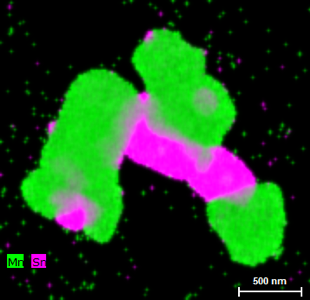
\includegraphics[width=0.29\textwidth]{\figurepath/batteries/edx_Sn_substitution.png}
};
\fill [color=Mn] (26em, -11.2em) rectangle (27.5em, -9.7em) node [pos=0.5, color=black, font=\small\bfseries] {Mn};
\fill [color=Sn] (27.5em, -11.2em) rectangle (29em, -9.7em) node [pos=0.5, color=black, font=\small\bfseries] {Sn};

\end{tikzpicture}

    \caption{(\textbf{a}) \gls{PXRD} patterns of 
\ce{Li_{1.2}Ni_{0.13}Co_{0.13}Mn_{0.54-x}Sn_xO2} for increasing values of 
Sn-substitution $x$. (\textbf{b}) Mixed (Mn, Sn) elemental \gls{EDX} map of representative 
LNMCS20 (x=0.108) particles, which demonstrates the presence of two different regions, a Mn-rich and Sn-rich one. Courtesy of Andreas Paulus (\textbf{a}) and Myl\`ene 
Hendrickx (\textbf{b}).} 
    \label{batteries:fig-Sn_experiment} 
\end{figure} 
 
To determine the \ce{Sn} solubility computationally, we investigate the 
thermodynamic stability of Sn-substituted structures versus their 
decomposition into an Mn-rich and Sn-rich phase. However, some approximations 
must be made in order to make the problem computationally feasible. First, 
including four different elements (\ce{Ni}, \ce{Mn}, \ce{Co} and \ce{Sn}) in 
our calculations would make both the number of configurations and reaction 
products prohibitively large, so we limit our study to the solubility of 
\ce{Sn} in \ce{Li_{1.2}Mn_{0.8}O2}. Considering the similar ionic radii of 
\ce{Mn^{4+}}, \ce{Co^{4+}} and \ce{Ni^{4+}}, this should not affect our 
conclusion significantly. Using this approximation, we first consider the 
following exsolution reaction: 
\begin{equation} 
 \ce{Li_{1.2}Mn_{0.8-x}Sn_xO2} \rightarrow  \left( 1 - \frac{x}{0.8} \right) 
\ce{Li_{1.2}Mn_{0.8}O2} +  \frac{x}{0.8} \ce{Li_{1.2}Sn_{0.8}O2}  
\end{equation} 
The \gls{PXRD} results indicate, however, that the final Sn-rich phase most likely 
corresponds to \ce{Li2SnO3} and, to a lesser extent, \ce{SnO}. This means that 
the following exsolution reaction is more probable: 
\begin{equation} \label{batteries:eq-exsolution} 
 \ce{Li_{1.2}Mn_{0.8-x}Sn_xO2} \rightarrow  \left( 1 - \frac{x}{0.8} \right) 
\ce{Li_{1.2}Mn_{0.8}O2} +  \frac{x}{0.8} \left[  0.6 \cdot \ce{Li2SnO3} + 0.2 
\cdot \ce{SnO} \right] 
\end{equation} 
 
Finally, there is another restriction to which our structures should adhere: 
based on the \gls{HAADF}-STEM results for several of the Sn-substituted samples, the 
honeycomb ordering of the \ce{Li}-TM/\ce{Sn} cations is largely 
maintained\footnote{Note that as the ratio of \ce{Li} over \gls{TM}/\ce{Sn} elements 
is smaller than 2, it is no longer possible to have a complete honeycomb 
ordering in the  \ce{Li}-TM/\ce{Sn} layer, as was the case for \ce{Li2MnO3}.}. 
This leads to the following construction of the \ce{Li_{1.2}Mn_{0.8}O2} 
structures:  
\begin{itemize} 
\item Start from the pristine primitive structure of O3-\ce{Li2MnO3}, with 
space group $C2/m$. 
\item Replace the \ce{Li} in the \ce{Li}/\ce{Mn} layer by a placeholder 
element, e.g. \ce{Lr}. This is just to keep track of which sites correspond to 
the \ce{Li} sites in the honeycomb layer. 
\item Make a 2$\times$2$\times$2 supercell. This size is chosen to get as close as possible 
to the experimental composition of \ce{Li}, without having to consider a unit 
cell size that is prohibitively large. 
\item Use the \texttt{Cathode.get\_cation\_configurations()} method to 
generate honeycomb-like structures by substituting the \ce{Lr} by \ce{Li} and 
\ce{Mn}, restricting the \ce{Li} concentration of the final configurations to 
closely match that of the experimental samples. 
\end{itemize} 
Because of the restrictions of the honeycomb pattern and \ce{Li} 
concentration, this method only results in 5 configurations, each with a 
composition that closely matches the experimental one: 
\ce{Li_{1.2083}Mn_{0.7917}O2} $\approx$ \ce{Li_{1.21}Mn_{0.79}O2}. To generate 
the \ce{Sn}-substituted structures, we consider each of the \ce{Mn} 
configurations, and once again use the 
\texttt{Cathode.get\_cation\_configurations()} method, this time partially 
substituting the \ce{Mn} elements by \ce{Sn}. For a single \ce{Sn} 
substitution in the supercell ($x = 0.042$), there are 47 possible 
\ce{Li}-\ce{Mn}-\ce{Sn}, which is still a manageable amount to handle with our 
configuration workflow. However, increasing the \ce{Sn} content further leads 
to 361/1867/7202 configurations for $x = 0.083/0.125/0.167$ respectively. 
Optimizing the geometry of all these configurations is clearly not possible, 
so we have to limit the number of configurations to a more manageable number.  
 
Before analyzing the reaction in Eq.~\ref{batteries:eq-exsolution}, it is 
important to confirm that the \ce{Sn}-rich phase is more likely to be a 
combination of \ce{Li2SnO3} and \ce{SnO} than \ce{Li_{1.2}Sn_{0.8}O2}. For 
this purpose, we first generate all \ce{Li}-\ce{Sn} configurations of 
\ce{Li_{1.2}Sn_{0.8}O2}, similar to the procedure described in the previous 
paragraph. Next, we optimize the geometry and calculate the energy of all 5 
configurations, along with the energies of \ce{Li2SnO3} and \ce{SnO}. Note 
that, similar to the \ce{Li}-rich \ce{Mn} structure, the composition of the 
configurations is closer to \ce{Li_{1.2083}Sn_{0.7917}O2}.This means that the 
effective decomposition reaction of interest is: 
\begin{equation} \label{batteries:eq-Sn-decomposition} 
\ce{Li_{1.2083}Sn_{0.7917}O2} \rightarrow  A  \cdot \ce{Li2SnO3} + B \cdot 
\ce{SnO}, 
\end{equation} 
where $A \approx 0.604$ and $B = 0.1875$. The corresponding formation energy 
is: 
\begin{equation} 
E_f = E(\ce{Li_{1.2083}Sn_{0.7917}O2}) - A \cdot E(\ce{Li2SnO3}) - B \cdot 
E(\ce{SnO}), 
\end{equation} 
which for the lowest energy configuration of \ce{Li_{1.2083}Sn_{0.7917}O2} is 
equal to 459~\si{\milli\electronvolt}. Considering the significantly larger 
energy of \ce{Li_{1.2083}Sn_{0.7917}O2} compared to \ce{Li2SnO3} and \ce{SnO}, 
it is reasonable to suggest that the \ce{Sn}-rich phase corresponds more 
closely to a combination of these end products. 
 
Finally, the exsolution reaction becomes: 
\begin{equation} \label{batteries:eq-exsolution_final} 
 \ce{Li_{1.21}Mn_{0.79-x}Sn_xO2} \rightarrow  \left( 1 - \frac{x}{0.79} 
\right) \ce{Li_{1.21}Mn_{0.79}O2} +  \frac{x}{0.79} \left[  0.604 \cdot 
\ce{Li2SnO3} + 0.1875 \cdot \ce{SnO} \right], 
\end{equation} 
with formation energy 
\begin{align} \label{batteries:eq-exsolution_final_formation} 
 E_f(x) = E(\ce{Li_{1.21}Mn_{0.79-x}Sn_xO2}) -  \left( 1 - \frac{x}{0.79} 
\right) E(\ce{Li_{1.21}Mn_{0.79}O2}) \nonumber \\ -  \frac{x}{0.79} \left[  0.604 \cdot 
E(\ce{Li2SnO3}) + 0.1875 \cdot E(\ce{SnO}) \right], 
\end{align} 
 
%However, instead of choosing the configurations randomly, it is better to 
% first rank the configurations by their electrostatic energy~\cite{Seo2016}, 
% calculated using the Ewald summation method. 
 
\begin{figure}[ht] 
\centering 
\captionsetup{width=0.9\linewidth}
\begin{tikzpicture}

\begin{axis}[
width=0.6\textwidth, height=6cm,
tick align=outside,
tick pos=left,
xmin=-0.02, xmax=0.25,
xtick={0, 0.05, 0.1, 0.15, 0.2, 0.25},
xticklabels={0, 0.05, 0.1, 0.15, 0.2, 0.25},
x grid style={white!69.0196078431373!black},
xlabel={$x$ in Li$_{1.2}$Mn$_{0.8-x}$Sn$_x$O$_3$},
xtick style={color=black},
ymin=0, ymax=40,
ytick={0, 10, 20, 30, 40},
yticklabels={0, 10, 20, 30, 40},
y grid style={white!69.0196078431373!black},
ylabel={$E_f$ (meV/atom)},
ytick style={color=black}, mark options={line width=1pt},
legend style={
at={(1, 1)}, anchor=north east, draw=none, fill=none, 
},
]
% This file was created by tikzplotlib v0.9.1.
\definecolor{color0}{rgb}{0.0392156862745098,0.313725490196078,0.52156862745098}

\addplot [only marks, mark=x, draw=color0, fill=color0, colormap/viridis]
table{%
x                      y
0 0
0 0.31117166666661
0 4.98020927083331
0 4.97478093749848
0 0.265032395832421
0.0416666666666667 15.2386898248987
0.0416666666666667 16.3269272207326
0.0416666666666667 20.5887670123978
0.0416666666666667 19.0977287832307
0.0416666666666667 20.8145852415643
0.0416666666666667 13.8410470123979
0.0416666666666667 8.8071136790645
0.0416666666666667 12.2127350332316
0.0416666666666667 8.43711711656525
0.0416666666666667 36.6861954498986
0.0416666666666667 6.6397675332307
0.0416666666666667 14.9104065957327
0.0416666666666667 11.4367493040649
0.0416666666666667 18.2227631582325
0.0416666666666667 2473.30455555406
0.0416666666666667 334.185957116565
0.0416666666666667 9.06490472073174
0.0416666666666667 15.1117193040654
0.0416666666666667 9.96965951239759
0.0416666666666667 8.60172638739798
0.0416666666666667 2520.53488586657
0.0416666666666667 15.8029944082322
0.0416666666666667 13.8394555540638
0.0416666666666667 12.8477562832315
0.0416666666666667 29.087034512398
0.0416666666666667 9.1810585748987
0.0416666666666667 10.1848557623977
0.0416666666666667 7.76613992906505
0.0416666666666667 8.60846419989791
0.0416666666666667 6.48778159573127
0.0416666666666667 10.2949804498983
0.0416666666666667 9.6029285748972
0.0416666666666667 22.6482043040647
0.0416666666666667 16.191564304065
0.0416666666666667 33.4274344082327
0.0416666666666667 12.4913215957313
0.0416666666666667 11.4895589915643
0.0416666666666667 1294.46220784573
0.0416666666666667 9.53851347073098
0.0416666666666667 1225.43296315823
0.0416666666666667 9.54966815823177
0.0416666666666667 23.638893366564
0.0416666666666667 3565.83250534573
0.0416666666666667 9.84547690823156
0.0416666666666667 9.94626607489934
0.0833333333333333 16.656766003962
0.0833333333333333 18.4626720456296
0.0833333333333333 16.8090592331291
0.0833333333333333 18.6703513164626
0.0833333333333333 18.1682511081294
0.0833333333333333 18.0458325664612
0.0833333333333333 17.3863199622952
0.0833333333333333 20.117021941463
0.0833333333333333 17.684096628962
0.0833333333333333 18.1234626706284
0.0833333333333333 18.7221944414626
0.0833333333333333 17.375109962295
0.0833333333333333 19.1593700664614
0.0833333333333333 15.3439350664615
0.0833333333333333 19.4292735039616
0.0833333333333333 14.488057774795
0.0833333333333333 16.9598531914625
0.0833333333333333 14.2287780872954
0.0833333333333333 15.7892975664622
0.0833333333333333 17.8882036081289
0.0833333333333333 17.953737878962
0.0833333333333333 17.6843527747954
0.0833333333333333 17.6074251706277
0.0833333333333333 18.4113550664622
0.0833333333333333 14.4141539206279
0.0833333333333333 13.8719118372956
0.0833333333333333 16.3145022539626
0.0833333333333333 15.9794942331291
0.0833333333333333 16.5889231914618
0.0833333333333333 16.4368435039608
0.0833333333333333 16.7142223581289
0.0833333333333333 19.3360607956274
0.0833333333333333 18.5732875664615
0.0833333333333333 19.8479183997942
0.0833333333333333 18.432045170629
0.0833333333333333 18.2946247539617
0.0833333333333333 16.3892895456288
0.0833333333333333 17.4936399622949
0.0833333333333333 18.2565055872959
0.0833333333333333 18.3334969414626
0.125 24.3105868705267
0.125 23.5059885371913
0.125 23.9258930163593
0.125 23.3498340580254
0.125 24.1912675996931
0.125 23.8893111413598
0.125 23.4280898913588
0.125 22.6777135371914
0.125 22.499776037193
0.125 22.1307042663592
0.125 21.8831239538591
0.125 23.9304347871925
0.125 23.1168334330252
0.125 23.947960724692
0.125 23.106370828859
0.125 23.409997078859
0.125 24.1138111413579
0.125 24.0050514538583
0.125 20.3486212455259
0.125 17.4866664538587
0.125 23.3119515580245
0.125 22.5319798913595
0.125 22.5026360371916
0.125 22.2292011413585
0.125 20.0877454121922
0.125 22.5481289538592
0.125 24.1253675996922
0.125 21.7470766621921
0.125 23.9000336413588
0.125 23.1665066621924
0.125 23.049980828858
0.125 23.9220918705256
0.125 23.2004475996912
0.125 20.7222964538594
0.125 20.8799168705265
0.125 21.3070517663598
0.125 21.8364700996925
0.125 25.0085330163592
0.125 25.7633991621922
0.125 19.379074370526
0.166666666666667 29.5897805495922
0.166666666666667 28.9658649245914
0.166666666666667 29.4282298204247
0.166666666666667 28.589117528758
0.166666666666667 28.8527641954253
0.166666666666667 27.1768472162583
0.166666666666667 28.1529396120912
0.166666666666667 27.9507608620917
0.166666666666667 27.0616686745924
0.166666666666667 28.051189507925
0.166666666666667 26.5412230495925
0.166666666666667 26.5753132579252
0.166666666666667 28.3969500287582
0.166666666666667 26.995791799592
0.166666666666667 24.4523859662578
0.166666666666667 21.8240141954253
0.166666666666667 23.5887031537572
0.166666666666667 24.159376278758
0.166666666666667 27.8743114870905
0.166666666666667 27.6722000287584
0.166666666666667 27.2112473204245
0.166666666666667 26.5492359662587
0.166666666666667 27.5873806537574
0.166666666666667 27.2332212787574
0.166666666666667 26.952836695425
0.166666666666667 25.4591486745919
0.166666666666667 27.5099319037593
0.166666666666667 27.5955348204255
0.166666666666667 26.7783336745917
0.166666666666667 23.5582121120905
0.166666666666667 27.9472236745923
0.166666666666667 25.5427305495917
0.166666666666667 25.7032762787595
0.166666666666667 27.7170583620907
0.166666666666667 24.6330739870912
0.166666666666667 27.2060858620917
0.166666666666667 27.9349440912582
0.166666666666667 32.1147976329246
0.166666666666667 26.296553362092
0.166666666666667 27.0430035704243
0.208333333333333 34.5013809994899
0.208333333333333 32.3486400619895
0.208333333333333 24.550888707823
0.208333333333333 27.8125543328236
0.208333333333333 28.2904161036561
0.208333333333333 28.8855487078226
0.208333333333333 27.0703182911567
0.208333333333333 26.4052621453224
0.208333333333333 26.5056138119895
0.208333333333333 24.1766436036559
0.208333333333333 27.8631812078216
0.208333333333333 27.0300987078236
0.208333333333333 32.8819201661559
0.208333333333333 31.5738886036558
0.208333333333333 31.1915719369895
0.208333333333333 30.010899853655
0.208333333333333 30.1398297494884
0.208333333333333 30.2911651661559
0.208333333333333 30.0623625619898
0.208333333333333 29.4394358953229
0.208333333333333 27.3426104786565
0.208333333333333 29.0714241244898
0.208333333333333 29.0610415203232
0.208333333333333 30.61190537449
0.208333333333333 27.8186945411565
0.208333333333333 31.2032990203224
0.208333333333333 31.198784541155
0.208333333333333 37.0649009994888
0.208333333333333 27.8186638119897
0.208333333333333 29.4655033953233
0.208333333333333 26.4986570411572
0.208333333333333 26.706616728656
0.208333333333333 31.7379253744892
0.208333333333333 29.9113002703222
0.208333333333333 27.2624965203234
0.208333333333333 32.8356161036552
0.208333333333333 32.3944814161563
0.208333333333333 31.2283648536549
0.208333333333333 25.2170041244901
0.791666666666667 123.123494798062
0.791666666666667 119.865812506394
0.791666666666667 120.188594902228
0.791666666666667 143.354342714726
0.791666666666667 114.716814068894
};

\end{axis}

\end{tikzpicture}

\caption{Calculated formation energies using 
Eq.~(\ref{batteries:eq-exsolution_final_formation}) for all configurations 
with $x = \{i/24|i=1,2,3,4,5\}$.} 
\label{batteries:fig-Sn_mixing} 
\end{figure} 
 
Figure~\ref{batteries:fig-Sn_mixing} shows the calculated formation energies 
for 40 configurations of the Sn substituted structures for each $x = 
\{i/24|i=1,2,3,4,5\}$, compared to their decomposition in 
\ce{Li_{1.21}Mn_{0.79}O2}, \ce{Li2SnO3} and \ce{SnO}. For the lowest Sn 
concentration, x = 0.042, the formation energy of the lowest energy 
configuration is only +6.5 meV/atom. This structure can 
reasonably be considered as metastable~\cite{Sun2016} and as such the 
formation of a single phase is feasible at low Sn concentrations. However, as 
the Sn-concentration $x$ is increased, the \ce{Li_{1.2}Mn_{0.8-x}Sn_xO2} 
configurations become more unstable, increasing the likelihood of a 
decomposition in \ce{Li_{1.2}Mn_{0.8}O2}, \ce{Li2SnO3} and \ce{SnO} phases, as 
observed in the \gls{PXRD} results for the high Sn concentration samples. Note that 
if the Sn substituted orderings are generated randomly, i.e. without 
respecting the honeycomb pattern, the energies are significantly higher 
compared to the honeycomb structures at each Sn concentration. This matches 
the preservation of the honeycomb ordering for the Sn substituted structure 
found for the \gls{HAADF}-STEM results. 
 
\resultsubsection{Influence of \ce{Mn^{4+}} substitution on oxygen stability \label{batteries:sec-dimer_substitution}}{https://github.com/mbercx/phd-thesis/tree/master/jupyter/batteries/README.md\#influence-of-mn4-substitution-on-oxygen-stability}{substitutions} 

The next question is whether the stability of the oxygen framework of 
\ce{Li2MnO3} can be improved by a local substitution of \ce{Mn^{4+}} by \ce{Sn^{4+}}. In order 
to make a fair comparison with the results presented in 
Sections~\ref{batteries:sec-oxidation} and \ref{batteries:sec-dimer}, we start 
from the 2$\times$2$\times$2 supercell of the charged O1-\ce{Li_{0.5}MnO3} structure. Based 
on the results of the previous section, only a limited amount of \ce{Sn} can 
be substituted in~\ce{Li2MnO3} before we expect the cathode to separate in several 
phases, and hence we simply substitute a single \ce{Mn} atom by \ce{Sn}. In 
light of the discussion of Section~\ref{batteries:sec-lirich},  however, we 
would not expect \ce{Sn} to be very effective in stabilizing the oxygen 
framework, as it is unable to oxidize beyond +4. Hence, we expand our search 
of suitable substitutions to \ce{V} and \ce{Mo}, two elements that permit 
higher states of oxidation and have shown promise in \ce{Li}-rich 
materials~\cite{Ma2014, Xiao2012}. Moreover, in order to study the influence of 
the exchange-correlation functional, we make a comparison between the \dft{PBEU}{} results and the 
recently introduced \dft{SCAN}{}. 
In contrast to \gls{PBE}+U, \gls{SCAN} does not rely on an element-dependent parameter, 
so it would be interesting to see if it produces a similar trend for the 
barrier of the various substituted elements.
This discussion, however, is left for the end of this section.
 
\begin{table}[ht] 
\centering 
\captionsetup{width=0.9\linewidth}
\renewcommand{\arraystretch}{1.3} 
\caption{Calculated absolute values of the magnetic moments for the discharged 
and charged for the \ce{Sn}/\ce{V}/\ce{Mo}-substituted structures, all 
expressed in Bohr magnetons $\mu_B$. For the oxygen, we make a distinction between the 
neighbors of the substituted element \ce{O_n} and other oxygen elements in 
the unit cell \ce{O_o}.} 
\label{batteries:tab-substitution_magmoms} 
\begin{tabular}{c c c c c c c} 
 & & \multicolumn{2}{c}{PBE+U} & & 
\multicolumn{2}{c}{SCAN}\\\cline{3-4}\cline{6-7} 
 & & discharged & charged & & discharged & charged \\\hline 
\multirow{3}{*}{Sn} & \multicolumn{1}{|c}{$|\mu|$ (\ce{Sn})} & 0.018 & 0.045 & 
& 0.017 & 0.064 \\ 
 & \multicolumn{1}{|c}{$|\mu|$ (\ce{O_n})} & 0.021 & 0.434 & & 0.020 & 0.355 
\\ 
 & \multicolumn{1}{|c}{$|\mu|$ (\ce{O_o})} & 0.000 & 0.463 & & 0.000 & 0.333 
\\\hline 
\multirow{3}{*}{V} & \multicolumn{1}{|c}{$|\mu|$ (\ce{V})} & 0.953 & 0.270 & & 
0.875 & 0.260 \\ 
 & \multicolumn{1}{|c}{$|\mu|$ (\ce{O_n})} & 0.012 & 0.329 & & 0.032 & 0.219 
\\ 
 & \multicolumn{1}{|c}{$|\mu|$ (\ce{O_o})} & 0.000 & 0.459 & & 0.000 & 0.322 
\\\hline 
\multirow{3}{*}{Mo} & \multicolumn{1}{|c}{$|\mu|$ (\ce{Mo})} & 1.792 & 0.172 & 
& 1.293 & 0.110 \\ 
 & \multicolumn{1}{|c}{$|\mu|$ (\ce{O_n})} & 0.028 & 0.208 & & 0.001 & 0.128 
\\ 
 & \multicolumn{1}{|c}{$|\mu|$ (\ce{O_o})} & 0.001 & 0.446 & & 0.000 & 0.310 
\\\hline 
\end{tabular} 
\end{table} 
 
Table~\ref{batteries:tab-substitution_magmoms} contains the magnetic moments 
and Fig.~\ref{batteries:fig-substitution_pdos_pbeu} shows the projected 
density of states near the Fermi level for the 
\ce{Sn}/\ce{V}/\ce{Mo}-substituted structures, both in the discharged and 
charged state. For \ce{Sn}, there are practically no states in near the Fermi 
level, which is not surprising considering that in a +4 oxidation state, Sn 
has donated its 5$s$ and 5$p$ valence electrons to the surrounding oxygen. 
This is also clear from the magnetic moments, which are close to zero for 
\ce{Sn} in both states of charge. Because of this inability of \ce{Sn} to 
oxidize further, the oxygen redox is similar to that of undoped \ce{Li2MnO3}. 
In light of this, it is unsurprising that the kinetic barrier for the A dimer 
in the 75\% charged Sn-doped structure is similar, even when one of the oxygen atoms neighbors the substituted 
\ce{Sn} (Fig.~\ref{batteries:fig-substitution_dimers}). 

\pagebreak[5] For \ce{V} and \ce{Mo}, the magnetic moments and projected density of states 
are also in the line of expectations. Both substituted elements show a clear 
change in their magnetic moment, indicating that they have oxidized further 
as the battery is charged. The neighboring oxygens \ce{O_n} also have a 
significantly lower magnetic moments compared to other oxygen atoms \ce{O_o} 
for the charged structure, confirming the decreased oxidation of the oxygen 
framework around the substituted element. Looking at the projected density of 
states in Fig.~\ref{batteries:fig-substitution_pdos_pbeu}, the \ce{V} and 
\ce{Mo} states are both right below the Fermi level, basically corresponding 
to donor levels in the band gap of the discharged \ce{Li2MnO3} structure. As 
\ce{Li} is removed from the structure, these states will be the first to be 
depopulated, which matches well with the picture provided by the magnetic 
moments. 
 
\begin{figure}[ht] 
\centering 
\captionsetup{width=0.9\linewidth}
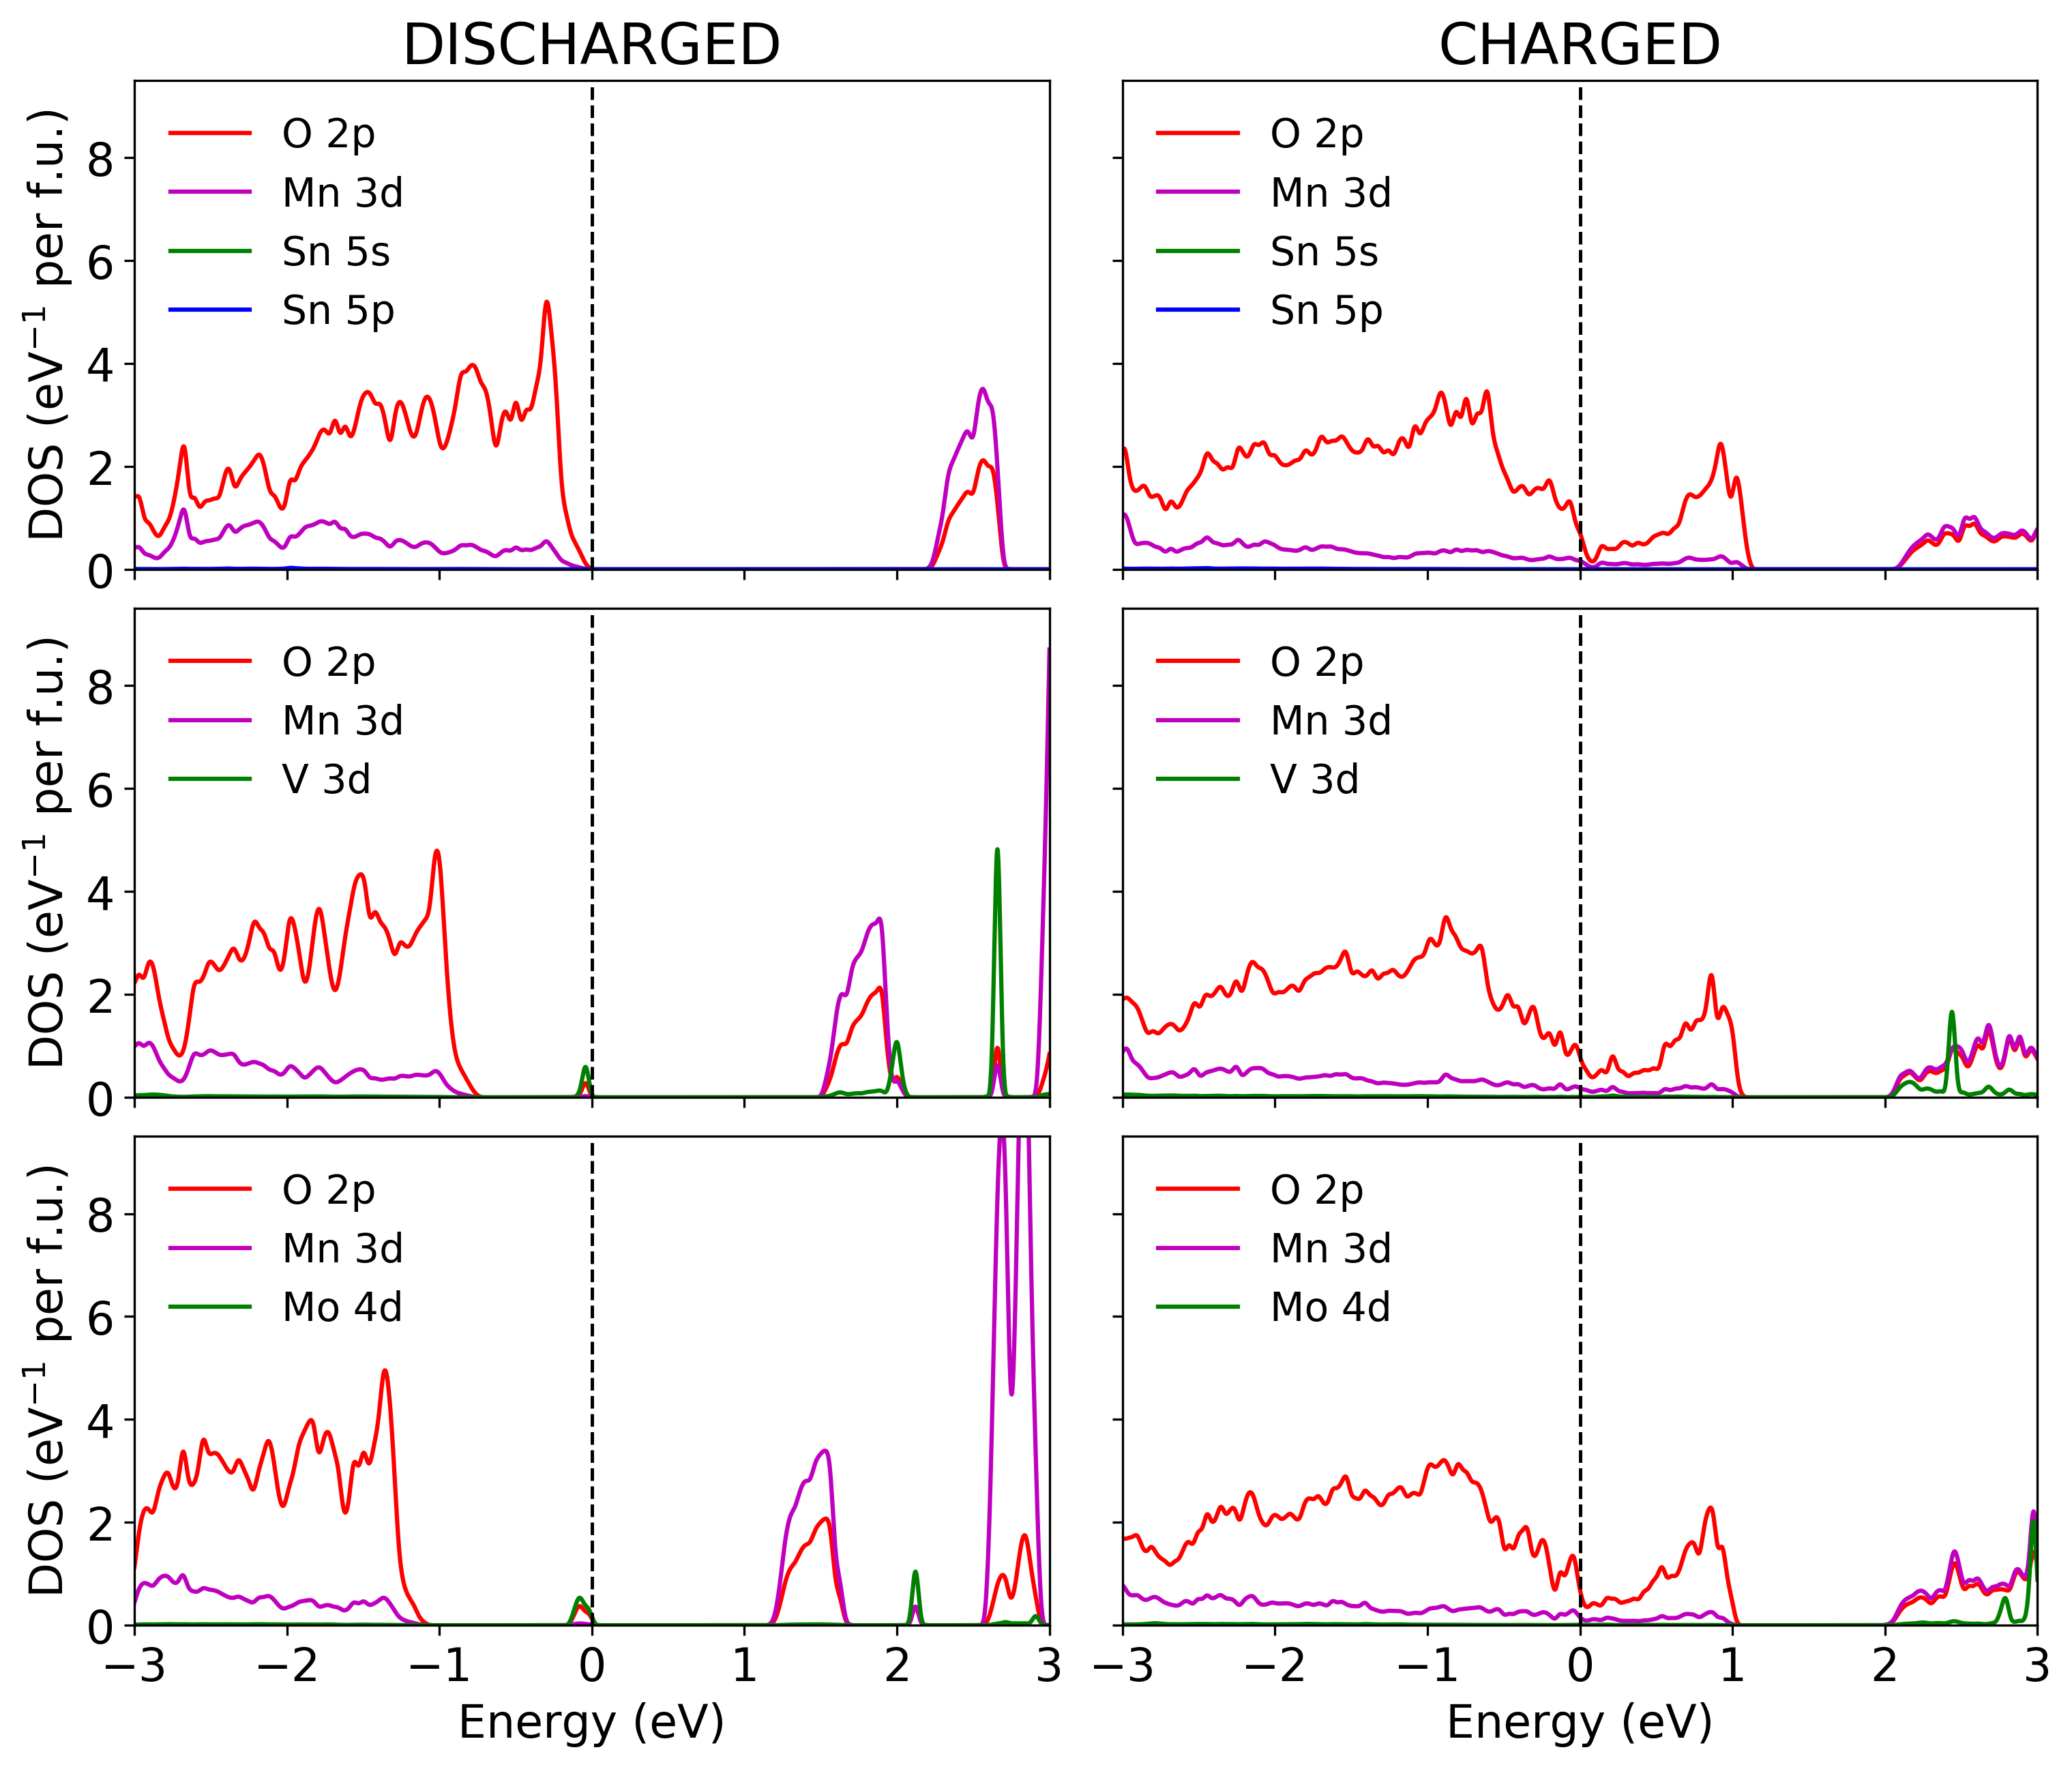
\includegraphics[width=\textwidth]{figures/batteries/substitution_pdos_pbeu.png} 
\caption{Projected density of states for the discharged (left) and charged 
(right) structures, for the 2$\times$2$\times$2 supercell of \ce{Li2MnO3} with a single 
substitution of \ce{Sn}, \ce{V} and \ce{Mo}.} 
\label{batteries:fig-substitution_pdos_pbeu} 
\end{figure} 

However, in contrast to \ce{Ir}, the increased propensity of \ce{V} and 
\ce{Mo} to oxidize does not seem to increase the stability of the surrounding 
oxygen framework. The kinetic barriers for the formation of the \textbf{A} 
dimer, shown in Fig.~\ref{batteries:fig-substitution_dimers}, is easily 
surmountable for both elements, and is in fact even lower compared to that of 
\ce{Li2MnO3}. Considering this, it would appear that neither the substitution 
of \ce{V} nor \ce{Mo} improves the stability of the oxygen framework, despite 
the fact that they are more likely to oxidize before the oxygen.  
 
\newpage
\begin{figure}[ht] 
\centering 
\captionsetup{width=0.9\linewidth}
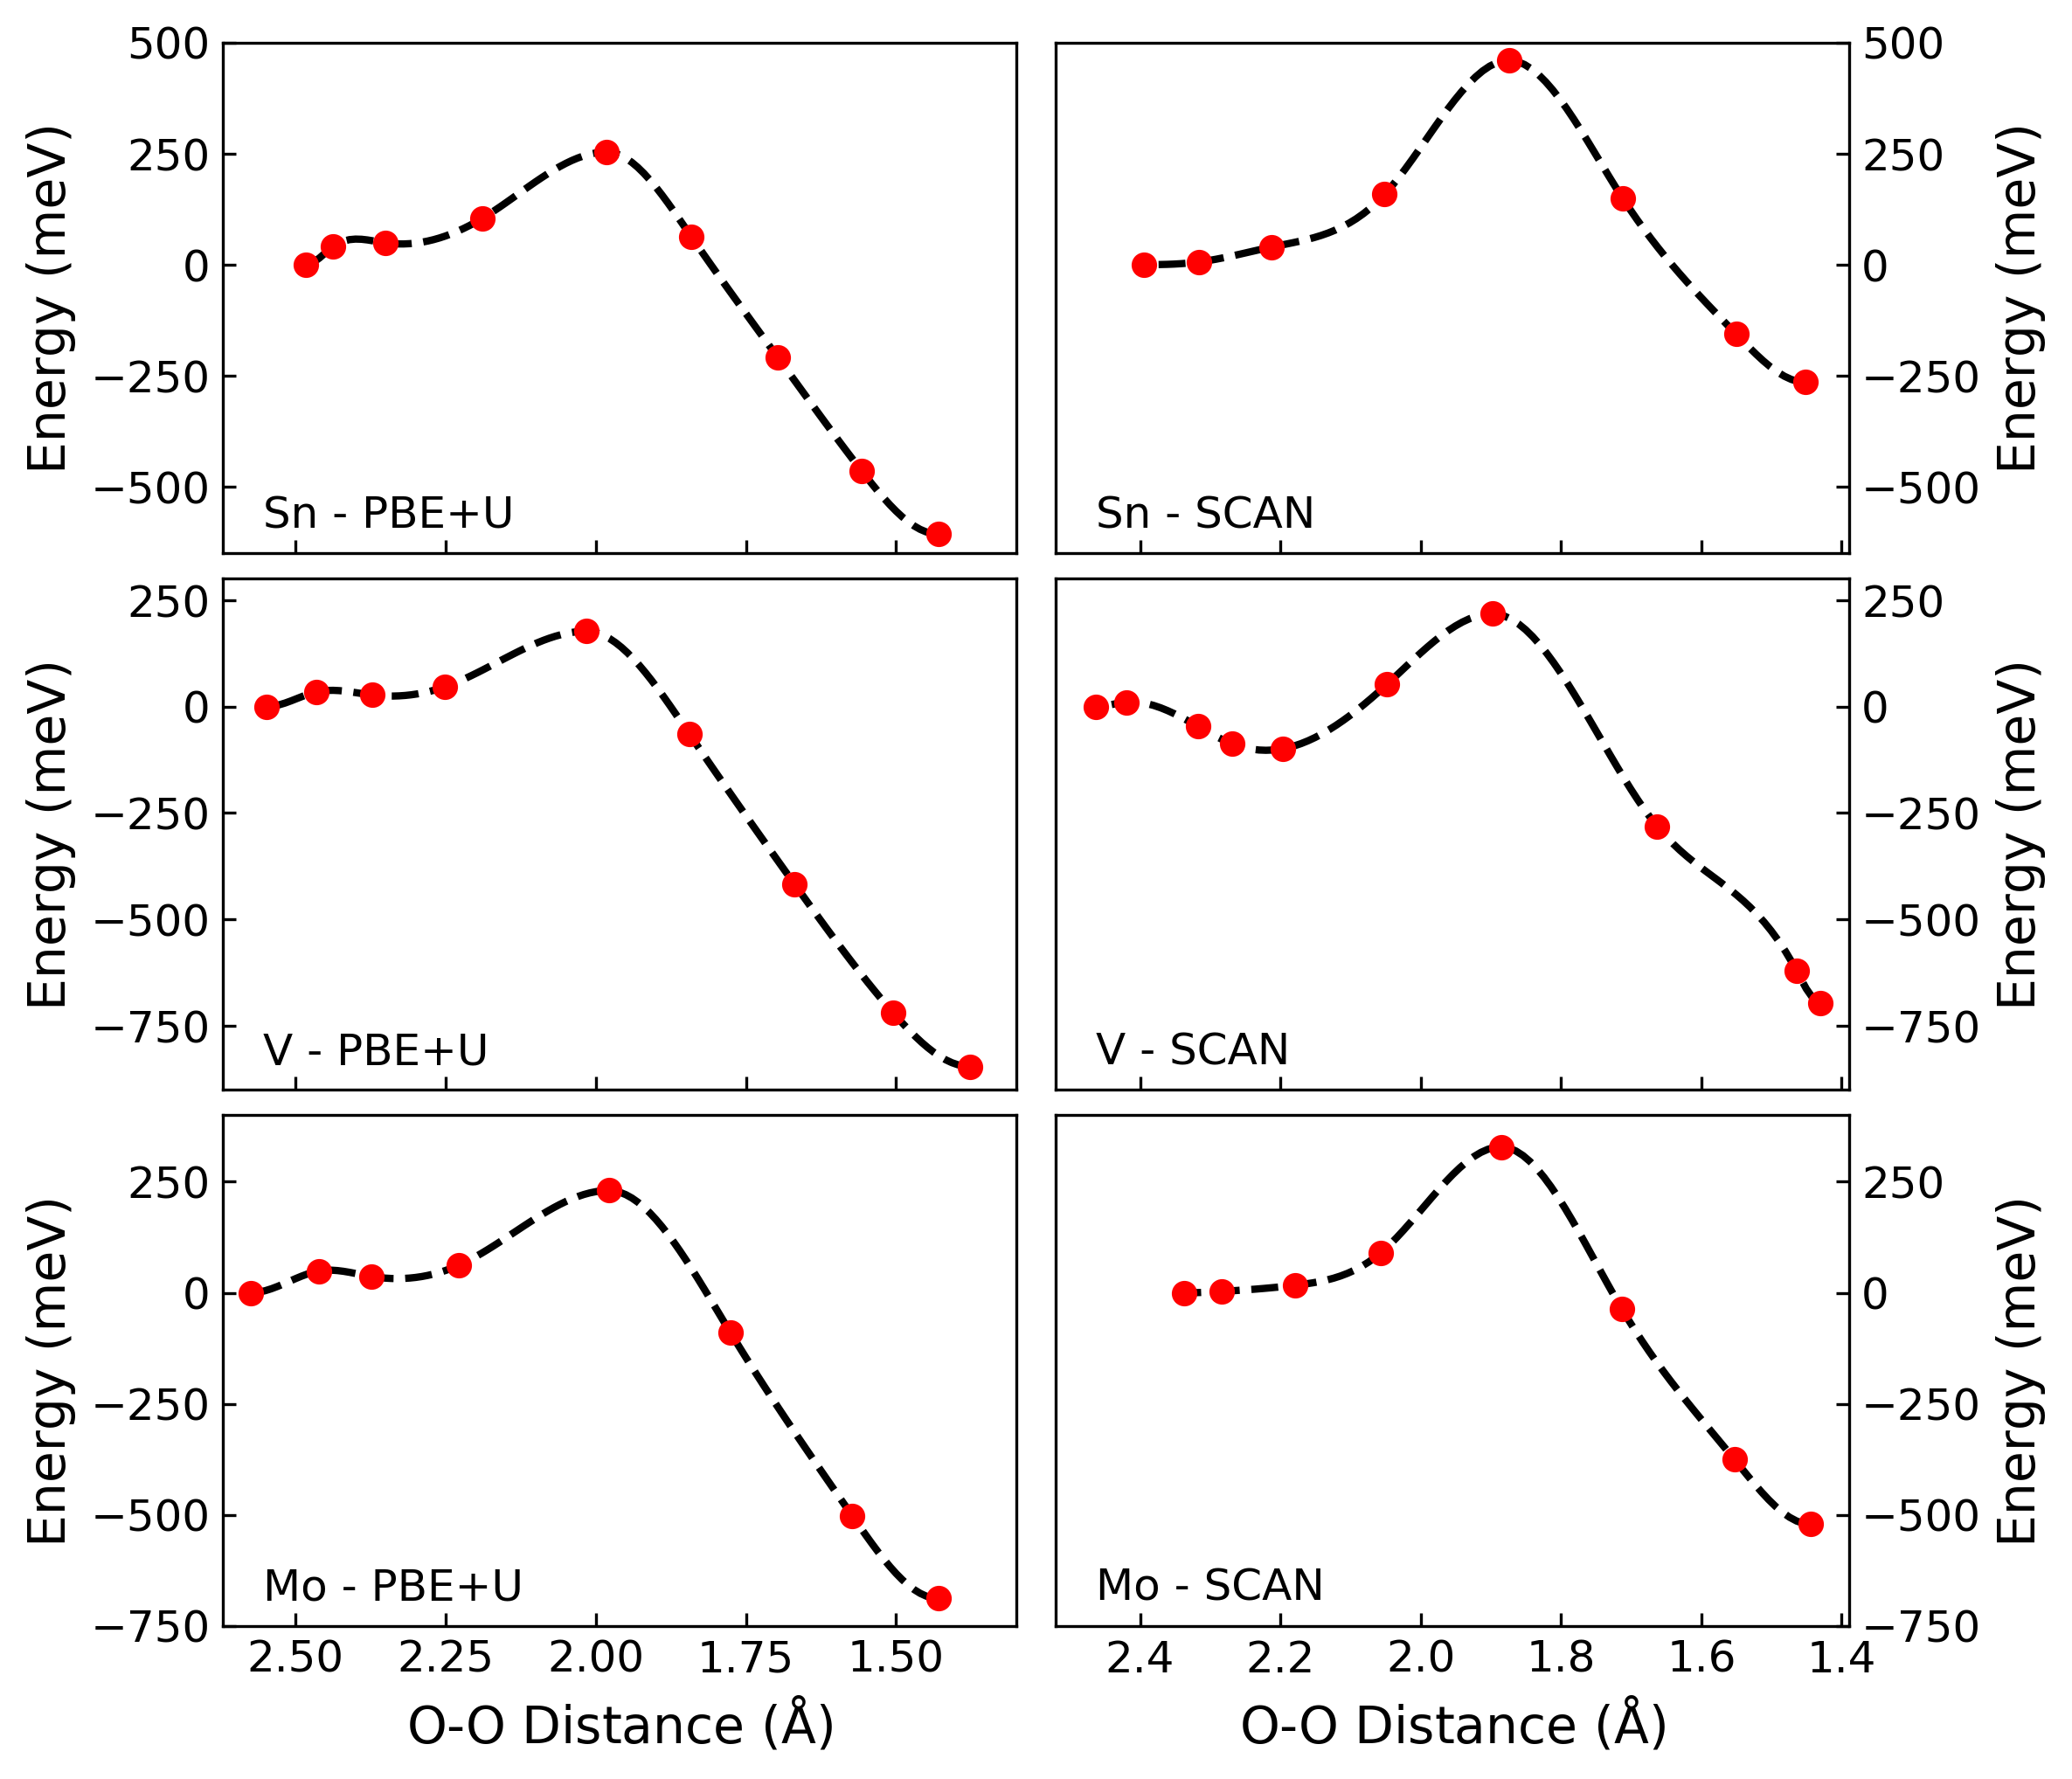
\includegraphics[width=0.85\textwidth]{figures/batteries/substitution_dimers.png} 
\caption{Kinetic barriers for the dimerization of oxygen neighboring \ce{Sn}, 
\ce{V} and \ce{Mo}, both for the \gls{PBE}+U and \gls{SCAN} functional.} 
\label{batteries:fig-substitution_dimers} 
\end{figure} 
 
Finally, we have also performed all of the calculations in this section with 
the recently published \dft{SCAN}{}, in order to compare the results with 
those of \dft{PBEU}{}. As \gls{SCAN} does not rely on specifying a parameter for each 
transition metal that can influence the oxidation state of the element, this 
provides an unbiased set of data to compare with. Looking at the magnetic 
moments in Table~\ref{batteries:tab-substitution_magmoms}, the discussion from 
the previous paragraphs remains largely intact. However, the magnetic moments 
on the oxygen atoms is decidedly lower compared to the \gls{PBE}+U results. One 
could argue that this indicates that our choice of Hubbard-U correction might 
have excessively localized the electrons around the transition metals, but a 
similar reduction in magnetic moments is found for the oxygen neighboring 
\ce{Sn}, for which we have applied no Hubbard-U correction. Moreover, our 
chosen U value for \ce{Mn} has been carefully benchmarked versus our previous 
results for \gls{HSE}06, which has demonstrated a good ability\footnote{Note that by 
tuning the fraction of exact exchange, it is possible to improve the accuracy 
of the \gls{HSE} functional further, but \dft{HSE06}{} (a = 0.25) does a fairly good job of 
reproducing experimental results.} for correcting the self-interaction error for 
battery cathodes~\cite{Seo2015}. Looking at the kinetic barriers in 
Fig.~\ref{batteries:fig-substitution_dimers}, \gls{SCAN} predicts a slightly 
increased barrier for each of the substituted elements, which could be linked 
to the reduced magnetic moment on \textit{all} oxygen atoms. Even this 
increased barrier is still relatively low, however, and hence not much of our 
analysis would if we would base it on the \gls{SCAN} results. 

\section{Polyborane solid electrolytes} \label{batteries:sec-solid_electrolyte}

Many of the current safety issues that plague Li-ion batteries, such as thermal runaway~\cite{Wang2012} and electrolyte decomposition~\cite{Lisbona2011}, are related to the use of a flammable liquid electrolyte~\cite{Liu2018, Ouyang2019}. To prevent hazardous incidents, complex packaging design is required at the cell, module and pack level~\cite{Dougthy2012} which increases the dead weight of the battery, reducing the energy density. A promising strategy for dealing with these issues is replacing the liquid electrolyte by a solid state ionic conductor. Besides improving the safety, solid state electrolytes also offer improved stability, which significantly increases the lifetime of the battery~\cite{Mauger2019}. Moreover, the electrochemical window of the solid electrolyte is typically larger, which allows for larger operating voltages~\cite{Li2014} and hence significant increases in the energy density. Finally, a solid electrolyte could also enable the development of Li-metal and Li-air batteries, as well as the miniaturization~\cite{Bates2000, Um2017} and three dimensional battery architectures~\cite{Long2004, Pearse2018}. 

A good solid electrolyte must demonstrate a high ionic conductivity and negligible electronic conductivity at the range of lithium activity and operating temperature of the battery~\cite{Knauth2009}. Other important properties include the chemical stability versus reactions at the electrode interfaces, and good mechanical properties in order to accommodate for the change in volume of the electrodes during the cycling of the battery~\cite{Koerver2018}. Different classes being considered as solid electrolytes include perovskite (e.g. LLTO~\cite{Inaguma1993}), NASICON (e.g. \ce{Na_{1+x}Zr_2Si_xP_{3-x}O_{12}} ($0 \leq x \leq 3$)~\cite{Hagman1968}) and garnet types (e.g. \ce{Li7La3Zr2O12} \cite{Murugan2007}). For a recent overview, we refer the reader to the review paper of Zheng et al.~\cite{Zheng2018}.

Here I present my contribution to the investigation of the theoretical principles behind the superionic conductivity of polyborane salts, a class of materials that has recently demonstrated significant potential as a solid electrolyte. This work was performed during a three month research stay at Lawrence Livermore National Laboratory, under the supervision of Dr. Brandon Wood and his group at the Materials Science Division. My work focused on setting up a toolbox for calculating such landscapes quickly, as described in the sections that follow and Section~\ref{automation:sec-landscape}. As such, the analysis presented in the following sections has been heavily inspired by the work of my collaborators, and largely corresponds to that of Dimitrievska et al.~\cite{Dimitrievska2018}. 

\subsection{Polyborane salts} \label{batteries:sec-polyborane_salts}

Polyborane salts have a rich chemistry which has been investigated for 60 years since dodecahydro\hyp\textit{closo}\hyp dodecaborate \ce{[B12H12]^{2-}} was synthesized by Pitochelli and Hawthorne~\cite{Pitochelli1960}. The first proposition of using polyborane salts as a solid electrolyte was made by Johnson and Whittingham~\cite{Johnson1980}, an idea that has been revived recently due to the increased interest in solid-state batteries by Udovic et al.~\cite{Udovic2014}. They found that above 529~\si{\kelvin}, \ce{Na2B12H12} undergoes a order-disorder phase transition which increases its ionic conductivity to $> 0.1~\si{\siemens\per\centi\meter}$, orders of magnitude larger than at room temperature. A similar phase transition was found to occur for \ce{Li2B12H12} at 600~\si{\kelvin}~\cite{Verdal2014}. Subsequently, Tang et al.~\cite{Tang2015} found that by substituting one of the \ce{B} atoms by \ce{C}, the temperature of the superionic transition is reduced drastically to 400~\si{\kelvin} and 380~\si{\kelvin} for \ce{LiCB11H12} and \ce{NaCB11H12}, respectively. Figure~\ref{batteries:fig-polyborane_structure} shows the structure of \ce{Li2B12H12} at room temperature, alongside the \ce{[B12H12]^{2-}} and \ce{[CB11H12]^{-}} anions. 

\begin{figure}
\centering
\captionsetup{width=0.9\textwidth}
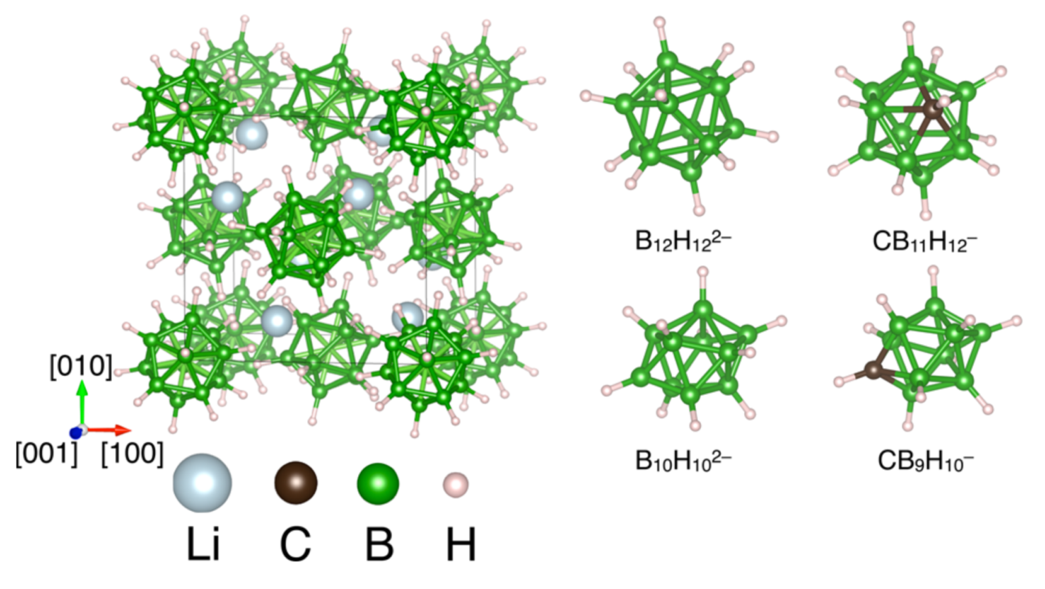
\includegraphics[width=0.7\textwidth]{\figurepath/batteries/polyborane_structure.png}
\caption{Crystalline \textit{fcc} structure of \ce{Li2B12H12} at room temperature.}
\label{batteries:fig-polyborane_structure}
\end{figure}

The high ionic conductivity of polyborane salts is believed to be connected to rapid reorientations of the anions~\cite{Skripov2015, Varley2016}, as well as the frustration between crystal symmetry and the local anion geometry as a result of long-range coulombic and short-range covalent-like interactions~\cite{Kweon2017}. Moreover, the lattice stacking of the large anions introduces spacious interstitial channels which facilitate cation conduction~\cite{Tang2015}, and because there are many more cation sites than cations, the structure can be interpreted as intrinsically high-vacancy, reducing the chance of migration channels being blocked. The interplay between the anion dynamics and cation mobility is complex, and I do not aim to provide a detailed explanation here. Instead, I will simply focus on my contribution to this line of research and its relation to other computational and experimental results. For more details, I refer the reader to the excellent analysis presented in the work of my collaborators~\cite{Varley2016, Kweon2017, Dimitrievska2018}.

\resultsubsection{Energy landscape of \ce{[CB11H12]^{-}} \label{batteries:sec-landscape}}{https://github.com/mbercx/phd-thesis/tree/master/jupyter/batteries/README.md\#energy-landscape-of-cb11h12-}{landscape}

In order to understand the local interaction between the anion and cation, I have calculated the energy landscape of the cation along a chain of ``wedges", i.e. curved 2D landscapes that connect the inequivalent facets of the anion (see Fig.~\ref{batteries:fig-cb11h12}a, as well as Fig.~\ref{automation:fig-landscape}). This involves calculating the energy of the anion-cation system with a static calculation for many different cation positions around the anion. Moreover, in order to be able to reasonably compare the energy landscapes of \ce{Li^+} versus \ce{Na^+}, I have calculated a reference energy based on the average of a spherical landscape with a radius of 8~\si{\angstrom}. Besides giving a better idea of the binding energy of the cation-anion pair, this also provides a measure for how easily the cation is able to hop back to an interstitial site, as the \textit{fcc} lattices of \ce{LiCB11H12} and \ce{NaCB11H12} have similar lattice constants (9.936~\si{\angstrom} and 10.066~\si{\angstrom}, respectively~\cite{Tang2015}). All of the landscapes presented in this section are compared with respect to this reference energy. The workflow used to calculate the landscapes is described in Section~\ref{automation:sec-landscape}, the computational details can be found in \link{appendix:sec-landscape}{corresponding section} in Appendix~\ref{appendix:sec-results}.

{
\begin{figure}[ht]
\centering
\begin{tikzpicture}

\node at (0.065\textwidth,-0.5) {\textsf{\textbf{a}}};

\node [anchor=north west] at (0.06\textwidth, 0) {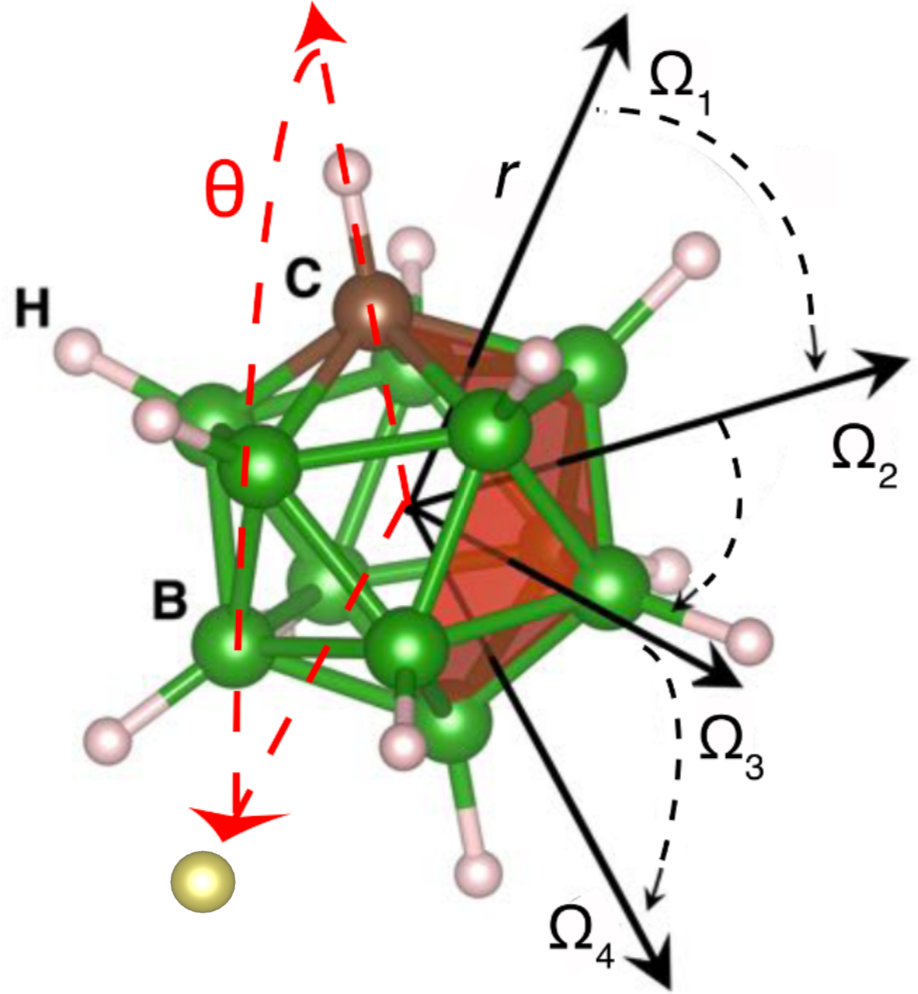
\includegraphics[width=0.31\textwidth]{\figurepath/batteries/anion_cb11h12.png}};

\node at (0.13\textwidth, -5.3) {\footnotesize \textsf{\textbf{Li/Na}}};

\node at (0.46\textwidth, -0.5) {\textsf{\textbf{b}}};

\node [anchor=north west] at (0.0\textwidth, -5.75) {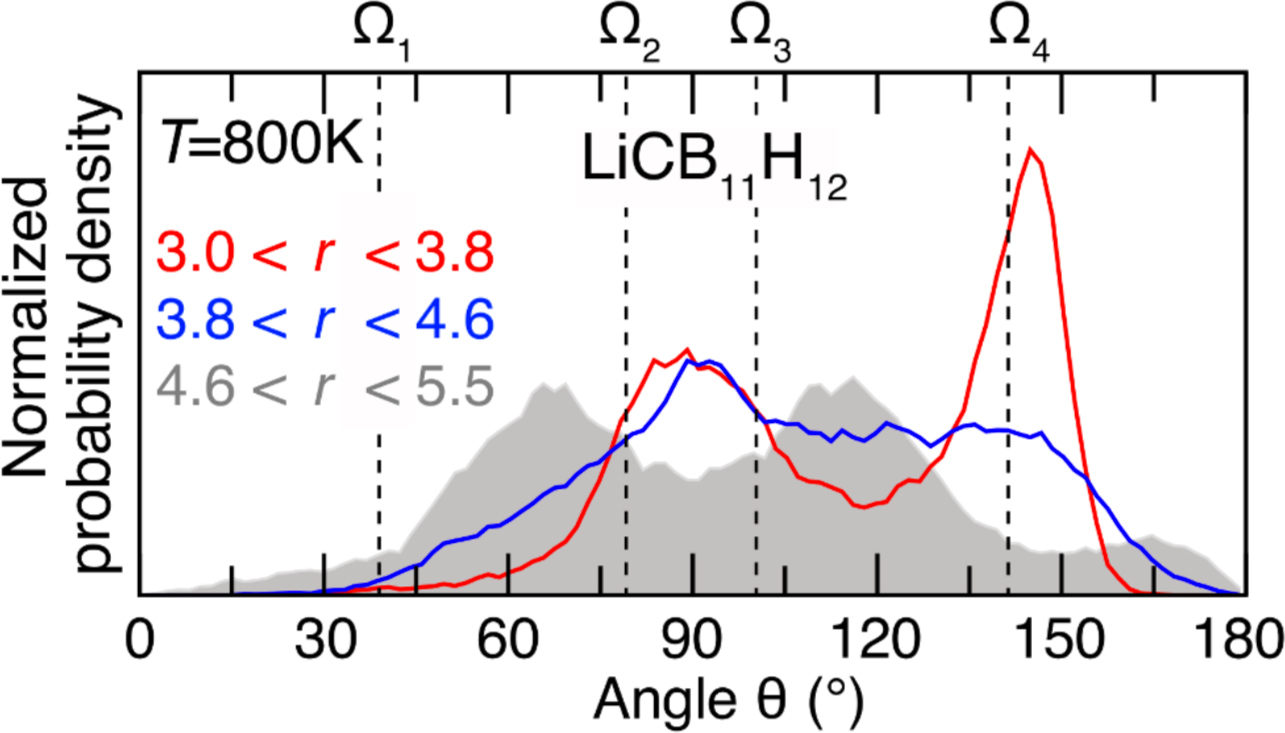
\includegraphics[width=0.44\textwidth]{\figurepath/batteries/aimd_cb11h12_Li.png}};

\node at (0.065\textwidth, -5.9) {\textsf{\textbf{c}}};

\node (landscapes) [anchor=north east] at (1.0\textwidth, -0.05) {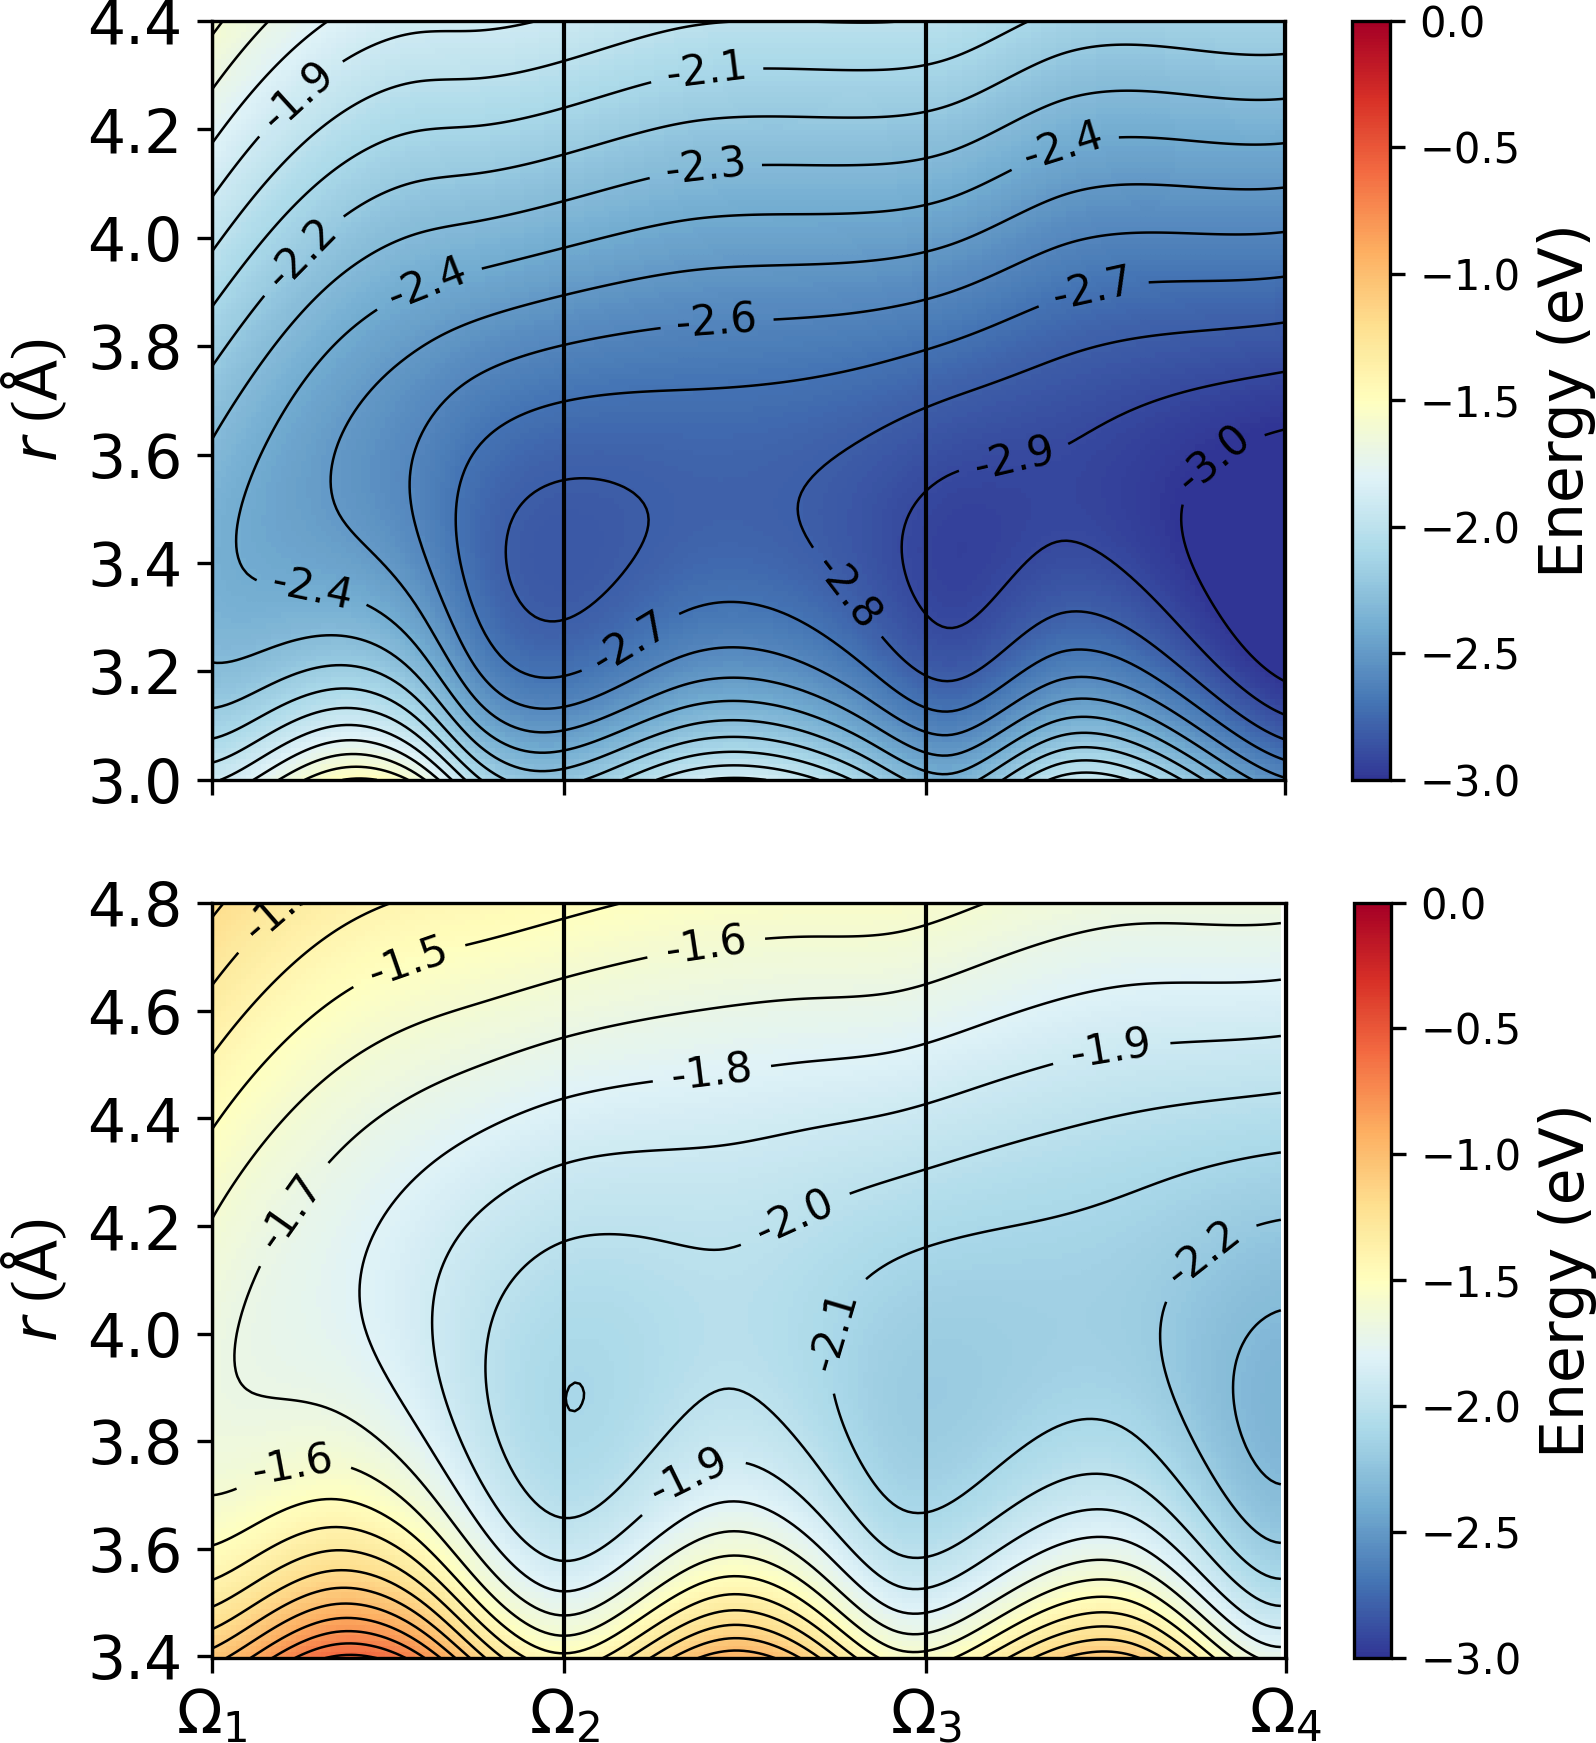
\includegraphics[width=0.54\textwidth]{\figurepath/batteries/ls_cb11h12.png}};

\node [fill=white, rounded corners, anchor=north west, font=\small\bfseries, text width=width("Na"), align=center] at (0.53\textwidth, -0.38) {\ce{Li}};

\node [fill=white, rounded corners, anchor=north west, font=\small\bfseries, text width=width("Na")] at (0.53\textwidth, -5.15) {\ce{Na}};


\end{tikzpicture}


\caption{(\textbf{a}) \ce{[CB11H12]^{-}} anion, with the symmetrically inequivalent facets colored red. Each of the facets corresponds to a binding site with direction $\Omega_i$ with respect to the center of the anion. (\textbf{b}) Angular distributions of the \ce{Li^+} cations derived from \gls{AIMD} simulations (Taken from~\cite{Dimitrievska2018}), where the angle $\theta$ is defined versus the C$_5$ axis connecting the C atom with the opposite B atom. (\textbf{c}) Calculated energy landscapes for \ce{Li^+} (top) and \ce{Na^+} (bottom) along wedges connecting the binding sites $\Omega_i$, relative to the spherical average at $8~\si{\angstrom}$.}
\label{batteries:fig-cb11h12}
\end{figure}
}

The resulting energy landscapes are compared with the ab initio molecular dynamics (AIMD) results from Dimitrievska et al.~\cite{Dimitrievska2018} in Fig.~\ref{batteries:fig-cb11h12}. The landscapes of \ce{Li^+} and \ce{Na^+} are qualitatively similar, and show a preference for the cations to bind at all-boron facets, where the depth of the energy wells is progressively larger for sites further removed from the \ce{C} atom. This result is in good agreement with the angle distributions obtained from the \gls{AIMD}, where we can see that the probability density is larger for angles corresponding to the all-boron docking sites ($\Omega_2$, $\Omega_3$ and $\Omega_4$), especially at smaller distances. At these distances, the likelihood of finding the cation near the $\Omega_4$ site is largest, which matches nicely with the increasing depth of the energy wells for sites further removed from \ce{C}. 

Moreover, the difference in the energy landscape between the \ce{C} facet ($\Omega_1$) and the lowest energy binding site ($\Omega_4$) is significant ($>0.6~\si{\electronvolt}$). As the anions undergo rapid reorientation in the superionic phase of both \ce{LiCB11H12} and \ce{NaCB11H12}~\cite{Dimitrievska2018}, this leads to a strongly fluctuating cation energy landscape close to the anions, which can push the cation back into interstitial sites. Hence, the substitution of \ce{B} by \ce{C} introduces a dipole in the anion, which in combination with its high rotational mobility can improve the ionic conductivity. This ``paddle wheel" effect was already described by Lunder et al. in the context of lithium sulphate materials~\cite{Lunden1995}, and is further supported by the by the \gls{AIMD} and quasielastic neutron scattering results of my collaborators~\cite{Dimitrievska2018}. 

Comparing the results for \ce{Li^+} and \ce{Na+}, it is clear that the cation is bound less strongly for \ce{Na^+}, as the wells corresponding to the binding sites are much higher in energy compared to the reference at 8~\si{\angstrom}. Moreover, the wells are also broader and located at a larger distance from the anion, which further indicates that cation can more easily be detached from the anion. This, in combination with the fact that the energy difference upon reorientation of the anion is similar to that for \ce{Li^+}, can explain the lower transition temperature to the superionic phase for \ce{NaCB11H12} (380~\si{\kelvin}) compared to \ce{LiCB11H12} (400~\si{\kelvin}).

\pagebreak[4]
\section{Conclusions and Outlook} 

In this chapter, I have made a comparison of the stability of the oxygen 
framework of two layered oxide materials which are being investigated for use 
as a cathode in \ce{Li}-ion batteries. An extensive study of the optimal 
lithium configuration at different states of charge shows that when the 
\ce{Li2MnO3} cathode is charged by 75\%, the stacking changes from O3 to O1.
Based on the charged structure, a comparison of the stability of the oxygen 
framework indicates that the formation of O-O dimers is both thermodynamically 
and kinetically viable for O1-\ce{Li_{0.5}MnO3}. For O1-\ce{Li_{0.5}IrO3}, the 
oxygen lattice is much more stable, either returning to its original 
state when perturbed, or resulting in a structure with an O-O dimer that is 
much higher in energy. This can in part be explained by the mixed redox 
process for \ce{Li2IrO3}, which is also confirmed by the calculated magnetic 
moments and calculated change in projected density of states.

The lack of O-O dimer formation in O1-\ce{Li_{0.5}IrO3} suggests that introducing 
transition metals in the Li-rich structure which allow for higher states of 
oxidation is a reasonable path for reducing the likelihood of the formation of 
O-O dimers, and the corresponding structural changes of the cathode that are 
tied to the detrimental voltage fade and oxygen evolution. However, other 
research has also shown that \ce{Sn} substitution can improve the structural 
stability. We have studied the solubility of \ce{Sn} in the 
\ce{Li_{1.2}Mn_{0.8}O2} structure, and find that only a limited substitution 
is thermodynamically feasible. Based on these results, we decided to study 
the influence of a single substitution of \ce{Mn} by \ce{Sn}, \ce{V} 
or \ce{Mo} on the oxygen oxidation and stability of its framework. Our results 
indicate that substituting \ce{Mn} by \ce{Sn} does little to change the 
properties of the oxygen framework, most likely due to their similar 
chemical inactivity during the charging process. For \ce{V} and \ce{Mo}, the 
substitution does reduce the oxidation of the neighboring oxygen atoms, 
but does not result in an improved stability. Instead, the kinetic barrier 
for dimerization is decreased further, indicating that the substitution 
destabilizes the structure instead. 

Although our results indicate that the formation of oxygen dimers in 
O1-\ce{Li_{0.5}MnO3} is likely to occur, we have yet to study its connection 
with the migration of Mn into the lithium layer. Other further investigations 
that could be interesting are the formation of oxygen dimers at the cathode 
surface, and subsequent evolution of \ce{O2} from the cathode into the 
electrolyte. So far, no substitution seems to be successful at stabilizing 
the structure. However, other approaches have been suggested for 
increasing the cycling properties of Li-rich materials, such as \ce{Ni} 
substitution in the \ce{Li} layer~\cite{Yang2017}, or the substitution of 
oxygen by fluor~\cite{Richards2017, Kapylou2017}. Both make sense in the context of 
our results. The most likely dimer according to our analysis is formed 
across the \ce{Li} layer, which would be inhibited by the presence of \ce{Ni}. 
Fluor, on the other hand, does not oxidize \ce{Mn} as much, leaving more 
room for the transition metal to oxidize as \ce{Li} is removed from the 
cathode. Further research is necessary to see if these ideas can properly 
stabilize the Li-rich cathode, opening it up to further development and 
integration in commercial applications.

Finally, we have calculated the energy landscapes of \ce{Li^+} and \ce{Na^+} 
cations around the carbonated polyborane salt anion \ce{[CB11H12]^{-}}. From 
the landscapes, it is clear than substituting a single boron by carbon introduces 
a dipole in the anion molecule, which in combination with the rapid reorientations 
of the anions results in a paddle wheel mechanism that improves the ionic 
conductivity of the material. This suggests a novel strategy for improving 
the properties of these materials for solid-state battery applications.
 
\clearpage
\pagestyle{biblio}
\printbibliography 
\clearpage

\end{refsection} 
